%% ============================================================
%% NTUST Master's Thesis, CSIE Department
%% National Taiwan University of Science and Technology
%% 國立臺灣科技大學 資訊工程系 碩士論文
%% ============================================================
\PassOptionsToPackage{hyphens}{url}
\documentclass[12pt,a4paper]{report}

%% ── Core packages ──────────────────────────────────────────
%% NTUST thesis margins: 3cm top and sides, 2cm bottom.
\usepackage[top=3cm, bottom=2cm, left=3cm, right=3cm]{geometry}
% Roman page numbers in the contents reach "xviii"; widen the number slot so
% the widest front-matter entry does not overflow its box.
\makeatletter
\renewcommand{\@pnumwidth}{2.2em}
\makeatother
\usepackage{setspace}
\usepackage{fontspec}
\usepackage{xeCJK}

%% ── Math ────────────────────────────────────────────────────
\usepackage{amsmath, amssymb}

%% ── Tables & Figures ────────────────────────────────────────
\usepackage{booktabs}
\usepackage{multirow}
\usepackage{longtable}
\usepackage{array}
\usepackage{ragged2e}
\usepackage{microtype}  % character protrusion: improves justification, suppresses under/overfull
\usepackage{graphicx}
\usepackage{float}
\usepackage{pdflscape}

%% ── Algorithms ──────────────────────────────────────────────
\usepackage{algorithm}
\usepackage{algorithmic}

%% ── References ──────────────────────────────────────────────
\usepackage[numbers,sort&compress]{natbib}
\bibliographystyle{unsrtnat}
\renewcommand{\bibname}{References}

%% ── Hyperlinks ──────────────────────────────────────────────
\usepackage[colorlinks=true,allcolors=black]{hyperref}
\hypersetup{
  pdftitle={Cloud GPU Rendering Scheduling Problem (CGRSP): A Mathematical Formulation and Empirical Evaluation on Heterogeneous GPU Fleets},
  pdfauthor={Michael},
  pdfsubject={Deadline-aware scheduling of 3D rendering workloads on heterogeneous, stochastically available cloud GPU fleets},
  pdfkeywords={cloud GPU scheduling, heterogeneous GPU fleet, discrete-event simulation, deadline-aware scheduling, RunPod, 3D rendering},
  pdflang={en}
}

%% ── Float tuning: avoid half-empty float pages ──────────────
\renewcommand{\floatpagefraction}{0.62}
\renewcommand{\topfraction}{0.85}
\renewcommand{\bottomfraction}{0.6}
\renewcommand{\textfraction}{0.1}
% Inline substitute for needspace.sty (not installed): break early if less
% than #1 of vertical space remains on the page.
\newcommand{\Needspace}[1]{\par\begingroup
  \setlength{\dimen0}{#1}%
  \vskip 0pt plus \dimen0\relax
  \penalty -100\relax
  \vskip 0pt plus -\dimen0\relax
\endgroup}

%% ── Headers / footers ───────────────────────────────────────
%% Past theses have no running header, just a centred page number.
\pagestyle{plain}

%% ── Caption style ───────────────────────────────────────────
%% Past theses: 12pt captions, plain (non-bold) label, centred.
\usepackage[font=normalsize,skip=12pt]{caption}

%% ── Enumitem ────────────────────────────────────────────────
\usepackage{enumitem}
\setlist[itemize]{leftmargin=2em}
\setlist[enumerate]{leftmargin=2em}

%% ── Fonts ───────────────────────────────────────────────────
\setmainfont{Times New Roman}
\setCJKmainfont[AutoFakeBold=3]{cwTeX Q Kai}
\setCJKmonofont{cwTeX Q Kai}

%% ── Line spacing ─────────────────────────────────────────────
%% Past theses use a 1.5 baseline stretch (~21.7pt leading at 12pt), a
%% visible skip between paragraphs, and a 2em paragraph indent, including
%% on the first paragraph after a heading (report class suppresses that
%% indent by default; indentfirst restores it to match past theses).
\usepackage{indentfirst}
\setstretch{1.5}
\setlength{\parskip}{11pt}
\setlength{\parindent}{2em}
% setspace force-singles floats, but the past theses keep the 1.5 stretch
% inside tables; route non-H floats back to the kernel implementation
% while leaving float.sty's [H] dispatcher in place.
\makeatletter
\let\@float@Hx\latex@xfloat
\makeatother
% Moderate line-breaking tolerance instead of blanket \sloppy: with microtype
% protrusion this clears overfull boxes without forcing loose (underfull) lines.
\tolerance=2500
\emergencystretch=3em
\hbadness=2500
\widowpenalty=10000
\clubpenalty=10000

%% ── Heading formatting ────────────────────────────────────────
%% Past theses: 24pt chapter titles and 18pt section titles.
\usepackage{titlesec}
\titleformat{\chapter}[block]
  {\normalfont\fontsize{24}{29}\selectfont\bfseries\filcenter}
  {Chapter \thechapter}{1em}{}
% -50pt cancels titlesec's inherited chapter drop so the title starts at
% the very top of the text block, as in the past theses.
\titlespacing*{\chapter}{0pt}{-50pt}{20pt}
\titleformat{\section}
  {\normalfont\fontsize{18}{22}\selectfont\bfseries\raggedright\hyphenpenalty=10000}{\thesection}{1em}{}
\titlespacing*{\section}{0pt}{14pt}{8pt}
\titleformat{\subsection}
  {\normalfont\Large\bfseries\raggedright\hyphenpenalty=10000}{\thesubsection}{1em}{}
\titlespacing*{\subsection}{0pt}{10pt}{5pt}
\titleformat{\subsubsection}
  {\normalfont\large\bfseries}{\thesubsubsection}{1em}{}
\titlespacing*{\subsubsection}{0pt}{8pt}{4pt}

%% ── Table of contents (matches past theses) ──────────────────
%% Chapter entries plain (not bold) with dotted leaders, like sections.
\makeatletter
\renewcommand*\l@chapter{\@dottedtocline{0}{0pt}{1.5em}}
\makeatother

%% ── Custom commands ──────────────────────────────────────────
\newcommand{\calJ}{\mathcal{J}}
\newcommand{\calN}{\mathcal{N}}
\newcommand{\calG}{\mathcal{G}}
\newcommand{\calK}{\mathcal{K}}

%% ── Auto-generated statistics macros (re-run generate_data.py) ────────
% AUTO-GENERATED by generate_data.py -- DO NOT EDIT
% Re-run: python3 generate_data.py
% Phase 3 (30-seed hectic day, C_max=5)
\newcommand{\SPTwait}{141.45}
\newcommand{\SPTmiss}{18.96}
\newcommand{\EDFmiss}{14.71}
\newcommand{\RescueWait}{146.32}
\newcommand{\RescueMiss}{13.56}
\newcommand{\FIFOwait}{167.93}
\newcommand{\FIFOmiss}{24.43}
\newcommand{\LCFmiss}{24.24}
\newcommand{\Balancedmiss}{25.25}
% Phase 3 t-test effect sizes (Cohen d)
\newcommand{\SPTFIFOwaitD}{-2.552}
\newcommand{\SPTFIFOmissD}{-1.351}
\newcommand{\EDFFIFOwaitD}{0.242}
\newcommand{\EDFFIFOmissD}{-2.668}
\newcommand{\RescueFIFOwaitD}{-2.336}
\newcommand{\RescueFIFOmissD}{-3.368}
% RH Phase 3 (30-seed hectic day)
\newcommand{\RHWait}{141.70}
\newcommand{\RHMiss}{9.60}
\newcommand{\RHFIFOwaitD}{-2.571}
\newcommand{\RHFIFOmissD}{-4.467}
\newcommand{\RHRescueWaitD}{-0.502}
\newcommand{\RHRescueMissD}{-1.287}
\newcommand{\RHFIFOwaitT}{-15.647}
\newcommand{\RHFIFOmissT}{-22.866}
\newcommand{\RHRescueMissT}{-5.839}
\newcommand{\RHRescueMissP}{0.000}
\newcommand{\RHRescueWaitT}{-2.402}
\newcommand{\RHRescueWaitP}{0.023}
% Wait ties asserted in the prose: RH vs SPT and CADR vs SPT+Rescue.
% Both are non-significant, which is what licenses the word "tied".
\newcommand{\RHSPTwaitT}{0.138}
\newcommand{\RHSPTwaitP}{0.891}
\newcommand{\RHSPTwaitD}{0.024}
\newcommand{\CADRRescueWaitT}{-1.237}
\newcommand{\CADRRescueWaitP}{0.226}
\newcommand{\CADRRescueWaitD}{-0.195}
% Random vs FIFO miss Cohen d and Random Phase 3 mean miss
\newcommand{\RandomFIFOmissD}{-0.344}
% SPT vs EDF miss p-value and Cohen d (EDF significantly lower since the
% 2026-07-19 complexity-mix fix; survives Holm)
\newcommand{\SPTEDFmissP}{0.000}
\newcommand{\SPTEDFmissD}{1.012}
% Phase 3 t-statistics and non-trivial p-values (for results tables)
\newcommand{\SPTFIFOwaitT}{-13.902}
\newcommand{\SPTFIFOmissT}{-7.394}
\newcommand{\RescueFIFOwaitT}{-12.249}
\newcommand{\RescueFIFOmissT}{-15.957}
\newcommand{\EDFFIFOwaitT}{1.478}
\newcommand{\EDFFIFOwaitP}{0.150}
\newcommand{\EDFFIFOmissT}{-15.326}
\newcommand{\RandomFIFOmissT}{-2.075}
\newcommand{\RandomFIFOmissP}{0.047}
\newcommand{\SPTEDFmissT}{4.931}
% Holm-Bonferroni family-wise correction over the pairwise t-test family
\newcommand{\HolmFamily}{24}
\newcommand{\HolmUncorrSig}{14}
\newcommand{\HolmNSig}{12}
\newcommand{\WilcoxHolmNSig}{12}
\newcommand{\SPTEDFmissWilcoxP}{0.0001}
\newcommand{\HolmMaxSigP}{0.000}
\newcommand{\HolmRemoved}{2}
\newcommand{\HolmRemovedUnprinted}{0}
% Phase 4 (30-day monthly, 10 replications)
\newcommand{\PhFourSPTwait}{101.92}
\newcommand{\PhFourSPTmiss}{12.86}
\newcommand{\PhFourRescueWait}{104.29}
\newcommand{\PhFourRescueMiss}{8.96}
\newcommand{\PhFourEDFwait}{116.69}
\newcommand{\PhFourEDFmiss}{8.92}
\newcommand{\PhFourFIFOmiss}{16.74}
\newcommand{\PhFourBalancedMiss}{16.55}
\newcommand{\PhFourLCFmiss}{16.50}
\newcommand{\PhFourRandomMiss}{15.62}
\newcommand{\PhFourRHWait}{103.73}
\newcommand{\PhFourRHMiss}{6.57}
% Phase 4 hectic-day sub-rates (from monthly_results.json)
\newcommand{\PhFourHecSPTmiss}{19.73}
\newcommand{\PhFourHecRescueMiss}{13.99}
\newcommand{\PhFourHecFIFOmiss}{25.11}
% Phase 2 (seed 42, single hectic-day run)
\newcommand{\PhTwoSPTwait}{140.02}
\newcommand{\PhTwoSPTmiss}{19.16}
\newcommand{\PhTwoEDFmiss}{12.11}
\newcommand{\PhTwoRescueWait}{144.02}
\newcommand{\PhTwoRescueMiss}{9.37}
\newcommand{\PhTwoFIFOmiss}{23.37}
\newcommand{\PhTwoUtilPct}{95.7}
% Phase 3 derived differences (rounded to integer minutes)
\newcommand{\SPTFIFOwaitDiffPct}{15.8}
% Cmax sensitivity (n=10 seeds, hectic day)
\newcommand{\CmaxSevenFIFOmiss}{6.3}
% Sensitivity: hectic day (30-seed mean, ~950 jobs)
\newcommand{\SensHecSPTwait}{141.4}
\newcommand{\SensHecSPTmiss}{19.0}
\newcommand{\SensHecFIFOmiss}{24.4}
\newcommand{\SensHecRHwait}{141.7}
\newcommand{\SensHecRHmiss}{9.6}
% Sensitivity: surge day (30-seed mean, ~730 jobs)
\newcommand{\SensSrgSPTmiss}{7.0}
\newcommand{\SensSrgEDFmiss}{1.6}
\newcommand{\SensSrgRescueMiss}{3.5}
% Deadline tightness sweep (surge day, 30 seeds each)
\newcommand{\DlTenEDFmiss}{0.62}
\newcommand{\DlTenSPTmiss}{3.31}
\newcommand{\DlThirtyEDFmiss}{3.45}
\newcommand{\DlThirtySPTmiss}{10.96}
\newcommand{\DlFiftyEDFmiss}{18.34}
\newcommand{\DlFiftySPTmiss}{18.91}
\newcommand{\DlSeventyEDFmiss}{34.64}
\newcommand{\DlSeventySPTmiss}{27.56}
\newcommand{\DlNinetyEDFmiss}{48.16}
\newcommand{\DlNinetySPTmiss}{36.74}
% Paired SPT vs EDF miss test at every sweep point (positive t = SPT
% higher, i.e. EDF lower). The sweep is where the two policies swap
% places, so the crossover claim needs a test at each point, not just
% the point estimates: at 50% tight the two are indistinguishable.
\newcommand{\DlTenSPTEDFmissT}{16.206}
\newcommand{\DlTenSPTEDFmissP}{p<10^{-15}}
\newcommand{\DlThirtySPTEDFmissT}{15.346}
\newcommand{\DlThirtySPTEDFmissP}{p<10^{-14}}
\newcommand{\DlFiftySPTEDFmissT}{0.520}
\newcommand{\DlFiftySPTEDFmissP}{p=0.61}
\newcommand{\DlSeventySPTEDFmissT}{-9.307}
\newcommand{\DlSeventySPTEDFmissP}{p<10^{-9}}
\newcommand{\DlNinetySPTEDFmissT}{-14.972}
\newcommand{\DlNinetySPTEDFmissP}{p<10^{-14}}
% Deadline sweep: baseline (FIFO/LCF/Balanced) range endpoints
\newcommand{\DlTenFIFOmiss}{5.27}
% Rescue threshold sensitivity (hectic day, 10 seeds)
\newcommand{\ThrSixtyMiss}{15.19}
\newcommand{\ThrOneEightyMiss}{11.66}
\newcommand{\ThrThreeHundredMiss}{12.01}
\newcommand{\ThrSixHundredMiss}{13.47}
\newcommand{\ThrDefaultGap}{1.81}
\newcommand{\ThrSixHundredWait}{144.71}
\newcommand{\ThrTwelveHundredMiss}{11.35}
\newcommand{\ThrMissSpread}{3.84}
% Phase 3 operational cost means (USD per 24h run) and spread
\newcommand{\RHcost}{6.35}
\newcommand{\RescueCost}{6.37}
\newcommand{\SPTcost}{6.34}
\newcommand{\LCFcost}{6.37}
\newcommand{\CostSpreadPct}{1.07}
% CADR Phase 3 (30-seed hectic day)
\newcommand{\CADRwait}{144.66}
\newcommand{\CADRmiss}{9.68}
\newcommand{\CADRcost}{6.36}
\newcommand{\CADRtard}{5.95}
\newcommand{\CADRtardReduction}{81}
% RH vs CADR on miss: paired test not significant; equivalence not established
\newcommand{\RHCADRmissT}{-0.111}
\newcommand{\RHCADRmissP}{0.912}
\newcommand{\RHCADRmissD}{-0.024}
% Phase 3 paired mean differences (first minus second scheduler), 95% t-CI, df=29
\newcommand{\SPTFIFOwaitMD}{-26.48}
\newcommand{\SPTFIFOwaitMDLo}{-30.37}
\newcommand{\SPTFIFOwaitMDHi}{-22.58}
\newcommand{\SPTFIFOmissMD}{-5.46}
\newcommand{\SPTFIFOmissMDLo}{-6.97}
\newcommand{\SPTFIFOmissMDHi}{-3.95}
\newcommand{\RescueFIFOwaitMD}{-21.61}
\newcommand{\RescueFIFOwaitMDLo}{-25.21}
\newcommand{\RescueFIFOwaitMDHi}{-18.00}
\newcommand{\RescueFIFOmissMD}{-10.86}
\newcommand{\RescueFIFOmissMDLo}{-12.26}
\newcommand{\RescueFIFOmissMDHi}{-9.47}
\newcommand{\EDFFIFOwaitMD}{2.30}
\newcommand{\EDFFIFOwaitMDLo}{-0.88}
\newcommand{\EDFFIFOwaitMDHi}{5.47}
\newcommand{\EDFFIFOmissMD}{-9.72}
\newcommand{\EDFFIFOmissMDLo}{-11.02}
\newcommand{\EDFFIFOmissMDHi}{-8.43}
\newcommand{\RandomFIFOmissMD}{-0.99}
\newcommand{\RandomFIFOmissMDLo}{-1.96}
\newcommand{\RandomFIFOmissMDHi}{-0.01}
\newcommand{\SPTEDFmissMD}{4.26}
\newcommand{\SPTEDFmissMDLo}{2.49}
\newcommand{\SPTEDFmissMDHi}{6.03}
\newcommand{\RHFIFOwaitMD}{-26.23}
\newcommand{\RHFIFOwaitMDLo}{-29.66}
\newcommand{\RHFIFOwaitMDHi}{-22.80}
\newcommand{\RHFIFOmissMD}{-14.83}
\newcommand{\RHFIFOmissMDLo}{-16.16}
\newcommand{\RHFIFOmissMDHi}{-13.51}
\newcommand{\RHRescueWaitMD}{-4.62}
\newcommand{\RHRescueWaitMDLo}{-8.56}
\newcommand{\RHRescueWaitMDHi}{-0.69}
\newcommand{\RHRescueMissMD}{-3.97}
\newcommand{\RHRescueMissMDLo}{-5.36}
\newcommand{\RHRescueMissMDHi}{-2.58}
\newcommand{\RHCADRmissMD}{-0.09}
\newcommand{\RHCADRmissMDLo}{-1.71}
\newcommand{\RHCADRmissMDHi}{1.53}
% Phase 3 tardiness for comparison set (mean, min)
\newcommand{\FIFOtard}{26.01}
\newcommand{\SPTtard}{12.02}
\newcommand{\EDFtard}{5.16}
\newcommand{\RescueTard}{5.89}
\newcommand{\RHtard}{31.84}
% Phase 4 CADR and tardiness macros
\newcommand{\PhFourCADRwait}{104.09}
\newcommand{\PhFourCADRMiss}{7.06}
\newcommand{\PhFourCADRTard}{6.27}
\newcommand{\PhFourRHtard}{19.07}
\newcommand{\PhFourEDFtard}{3.77}
\newcommand{\PhFourFIFOtard}{18.02}
\newcommand{\PhFourSPTtard}{10.69}
\newcommand{\PhFourRescueTard}{5.19}
% Sensitivity: hectic day CADR
\newcommand{\SensHecCADRwait}{144.7}
\newcommand{\SensHecCADRmiss}{9.7}
% CADR-order-only ablation (isolation of cost-aware placement)
\newcommand{\CADROOmiss}{10.16}
\newcommand{\CADROOwait}{145.96}
\newcommand{\CADROOtard}{6.59}
% CR* sensitivity prose macros. CRStarBestCR is the argmin, so the
% prose never has to name the winning threshold by hand, and
% CRStarDefaultGap is how far the shipped default sits above it.
\newcommand{\CRStarBestMiss}{9.28}
\newcommand{\CRStarBestCR}{3}
\newcommand{\CRStarDefaultMiss}{9.28}
\newcommand{\CRStarDefaultGap}{0.00}
\newcommand{\CRStarMissSpread}{2.19}
% RH anticipation (reservation) payoff: surge below saturation
\newcommand{\ResSurgeOffMiss}{6.42}
\newcommand{\ResSurgeOnMiss}{1.33}
\newcommand{\ResSurgeOffTight}{31.99}
\newcommand{\ResSurgeOnTight}{6.62}
\newcommand{\ResSurgeOffWait}{96.87}
\newcommand{\ResSurgeOnWait}{108.76}
\newcommand{\ResSurgeOnLoose}{0.01}
\newcommand{\ResHecticGateMiss}{9.60}
% Sensitivity: surge day RH (anticipation active below saturation)
\newcommand{\SensSrgRHmiss}{1.3}
\newcommand{\SensSrgRHwait}{108.8}
% Surge-day wait range over the seven policies and five fractions of the deadline-tightness sweep (ch5 prose)
\newcommand{\SensSrgWaitLo}{95}
\newcommand{\SensSrgWaitHi}{99}
% Surge-day wait range over all ten schedulers in the day-type table (ch5 and ch6 prose)
\newcommand{\SensSrgDayWaitLo}{95}
\newcommand{\SensSrgDayWaitHi}{109}
\newcommand{\PriorGateLambda}{0.0634}
\newcommand{\PriorSurgeCrossX}{3.2}
\newcommand{\PriorGateShortfall}{37}
\newcommand{\PriorHecUnderMiss}{22.12}
\newcommand{\PriorHecUnderWait}{208.76}
\newcommand{\CmaxTenRHwait}{13.1}
\newcommand{\CmaxTenOtherWaitLo}{7.4}
\newcommand{\CmaxTenOtherWaitHi}{9.0}
\newcommand{\CRStarWaitSpread}{2.8}
% Adaptive EDF-SPT hybrid (Phase 3 hectic 30-seed, Phase 4 monthly, sensitivity)
\newcommand{\AdaptiveWait}{169.67}
\newcommand{\AdaptiveMiss}{12.62}
\newcommand{\AdaptiveTard}{4.91}
\newcommand{\PhFourAdaptiveWait}{116.81}
\newcommand{\PhFourAdaptiveMiss}{7.53}
\newcommand{\PhFourAdaptiveTard}{3.51}
\newcommand{\SensSrgAdaptiveMiss}{1.5}

\newcommand{\MonthResWaitDelta}{2.20}
\newcommand{\MonthResWaitP}{p=0.006}
\newcommand{\MonthResMissDelta}{0.76}
\newcommand{\MonthResMissP}{p<10^{-4}}
\newcommand{\MonthResTardDelta}{2.29}
\newcommand{\MonthResTardP}{p<10^{-3}}
\newcommand{\MonthResOffWait}{101.53}
\newcommand{\MonthResOffMiss}{7.33}
\newcommand{\SparseExposureLo}{20.63}
\newcommand{\SparseExposureHi}{23.23}
\newcommand{\SparseSigmaHighP}{0.465}
\newcommand{\SparseSigmaHighAdjustedP}{1.000}
\newcommand{\SparseBaseRHMiss}{8.46}
\newcommand{\SparseBaseCADRMiss}{9.28}
\newcommand{\SparseMeanLowRHMiss}{7.07}
\newcommand{\SparseMeanLowCADRMiss}{5.17}
\newcommand{\SparseMeanHighRHMiss}{10.44}
\newcommand{\SparseMeanHighCADRMiss}{10.80}
\newcommand{\SparseSigmaLowRHMiss}{9.56}
\newcommand{\SparseSigmaLowCADRMiss}{10.05}
\newcommand{\SparseSigmaHighRHMiss}{8.86}
\newcommand{\SparseSigmaHighCADRMiss}{7.71}
\newcommand{\KsBaseFIFOMiss}{23.67}
\newcommand{\KsBaseSPTMiss}{17.65}
\newcommand{\KsBaseEDFMiss}{12.68}
\newcommand{\KsBaseSPTRescueMiss}{13.47}
\newcommand{\KsBaseRHMiss}{8.46}
\newcommand{\KsBaseCADRMiss}{9.28}
\newcommand{\KsBaseRHvCADRp}{0.648}
\newcommand{\KsAdjLowFIFOMiss}{23.67}
\newcommand{\KsAdjLowSPTMiss}{19.55}
\newcommand{\KsAdjLowEDFMiss}{14.19}
\newcommand{\KsAdjLowSPTRescueMiss}{13.55}
\newcommand{\KsAdjLowRHMiss}{9.65}
\newcommand{\KsAdjLowCADRMiss}{10.02}
\newcommand{\KsAdjLowRHvCADRp}{0.801}
\newcommand{\KsAdjHighFIFOMiss}{23.67}
\newcommand{\KsAdjHighSPTMiss}{20.66}
\newcommand{\KsAdjHighEDFMiss}{13.67}
\newcommand{\KsAdjHighSPTRescueMiss}{15.52}
\newcommand{\KsAdjHighRHMiss}{10.51}
\newcommand{\KsAdjHighCADRMiss}{11.82}
\newcommand{\KsAdjHighRHvCADRp}{0.204}
\newcommand{\KsUninfFIFOMiss}{23.67}
\newcommand{\KsUninfSPTMiss}{23.96}
\newcommand{\KsUninfEDFMiss}{13.07}
\newcommand{\KsUninfSPTRescueMiss}{18.22}
\newcommand{\KsUninfRHMiss}{13.02}
\newcommand{\KsUninfCADRMiss}{14.24}
\newcommand{\KsUninfRHvCADRp}{0.399}
\newcommand{\KsSlowFIFOMiss}{25.92}
\newcommand{\KsSlowSPTMiss}{20.76}
\newcommand{\KsSlowEDFMiss}{16.76}
\newcommand{\KsSlowSPTRescueMiss}{14.56}
\newcommand{\KsSlowRHMiss}{9.28}
\newcommand{\KsSlowCADRMiss}{11.25}
\newcommand{\KsSlowRHvCADRp}{0.003}
\newcommand{\CapBoundMeanPct}{0.00}
\newcommand{\CapBoundMaxMisses}{0}
\newcommand{\RelaxEDFMeanPct}{0.00}
\newcommand{\BetaQuarterCompletedPct}{19}
\newcommand{\BetaHalfCompletedPct}{90}
\newcommand{\BetaThreeQRHmiss}{44.3}
\newcommand{\BetaThreeQRescueMiss}{49.2}
\newcommand{\BetaThreeQCADRmiss}{48.4}
\newcommand{\BetaThreeQFIFOmiss}{57.0}
\newcommand{\BetaUpRHmiss}{5.44}
\newcommand{\BetaUpSPTmiss}{6.38}
\newcommand{\BetaHalfMinEffMiss}{89.6}
\newcommand{\BetaThreeQuarterMinEffMiss}{44.3}
\newcommand{\BetaThreeQuarterMaxEffMiss}{57.2}
\newcommand{\BetaRHvCADRt}{-7.26}
\newcommand{\BetaRHvCADRp}{p<10^{-7}}
\newcommand{\BetaRHvRescueT}{-8.83}
\newcommand{\BetaRHvRescueP}{p<10^{-8}}
\newcommand{\RevRHmiss}{6.25}
\newcommand{\RevCADRmiss}{2.40}
\newcommand{\RevRescueMiss}{3.37}
\newcommand{\RevSPTmiss}{9.96}
\newcommand{\RevFIFOmiss}{17.73}
\newcommand{\RevEDFmiss}{4.84}
\newcommand{\NoPriorRHmiss}{9.53}
\newcommand{\NoPriorRHwait}{141.18}
\newcommand{\RevRHvCADRt}{7.95}
\newcommand{\RevRHvCADRp}{p<10^{-8}}
\newcommand{\NoPriorDiffPp}{0.07}
\newcommand{\NoPriorT}{0.11}
\newcommand{\NoPriorP}{p=0.91}
\newcommand{\PswpBestP}{10}
\newcommand{\PswpBestMiss}{11.48}
\newcommand{\PswpBaseMiss}{11.48}
\newcommand{\PswpSpread}{2.57}
\newcommand{\PswpBestTard}{4.42}
\newcommand{\PswpBestTardVal}{3.86}
\newcommand{\PswpBestTardP}{50}
\newcommand{\PswpVsRHdiff}{+3.02}
\newcommand{\PswpVsRHt}{2.06}
\newcommand{\PswpVsRHp}{p=0.069}
\newcommand{\TFreeCollapsedPct}{85}
\newcommand{\DiagRHTightLo}{66}
\newcommand{\DiagRHTightHi}{68}
\newcommand{\DiagRHMissLo}{70}
\newcommand{\DiagRHMissHi}{83}
\newcommand{\DiagRHTightLateLo}{472}
\newcommand{\DiagRHTightLateHi}{478}
\newcommand{\DiagCADRTightTotal}{1}
\newcommand{\DiagBandLo}{129}
\newcommand{\DiagBandHi}{169}
\newcommand{\MeanSvcWaitMaxPct}{1.6}
\newcommand{\MeanSvcMissMaxRelPct}{11}
\newcommand{\MeanSvcRHMiss}{9.33}
\newcommand{\MeanSvcCADRMiss}{9.90}
\newcommand{\MeanSvcRHvCADRp}{0.35}


%% ── Metadata ─────────────────────────────────────────────────
\title{Cloud GPU Rendering Scheduling Problem (CGRSP):\\
A Mathematical Formulation and Empirical Evaluation\\
on Heterogeneous GPU Fleets}
\author{Michael}
\date{January 2027}

%% ─────────────────────────────────────────────────────────────
\newcommand{\doi}[1]{doi:~\href{https://doi.org/#1}{\nolinkurl{#1}}}
\begin{document}

%% ── Roman numerals for front matter ─────────────────────────
%% Like the past theses: cover unnumbered, roman numerals shown from the
%% Chinese abstract onward, arabic from Chapter 1.
\pagenumbering{Roman}

\begin{titlepage}
% The cover uses explicit \fontsize baselines; suppress the global 1.5
% stretch and parskip inside this group so it stays a single page.
\singlespacing
\setlength{\parskip}{0pt}
\thispagestyle{empty}
\vspace*{-0.4cm}

\noindent
\begin{tabular}{@{}c@{\hspace{1.5cm}}c@{}}
\raisebox{-0.5\height}{
\includegraphics[width=2.8cm]{figures/ntust_logo_badge.png}} &
\begin{tabular}[c]{@{}c@{}}
{\fontsize{24}{28}\selectfont 國立臺灣科技大學}\\
{\fontsize{24}{28}\selectfont 資訊工程系}
\end{tabular}
\end{tabular}

\vspace{0.7cm}
\noindent\rule{\textwidth}{3pt}

\vspace{0.4cm}
\begin{center}
{\fontsize{24}{28}\selectfont 碩士學位論文}
\end{center}

\vspace{0.4cm}
\begin{center}
{\fontsize{22}{27}\selectfont 雲端GPU渲染排程問題 (CGRSP)：異質GPU叢集之數學建模與實驗評估\par}
\end{center}

\vspace{0.6cm}
\begin{center}
{\fontsize{22}{27}\selectfont\bfseries Cloud GPU Rendering Scheduling Problem (CGRSP): A Mathematical Formulation and Empirical Evaluation on Heterogeneous GPU~Fleets\par}
\end{center}

\vspace{2.7cm}
\begin{center}
\begingroup
\fontsize{17}{21}\selectfont
\newlength{\coverlabelwidth}
\settowidth{\coverlabelwidth}{共同指導教授}
\begin{tabular}{@{}l@{}}
\makebox[\coverlabelwidth][l]{研究生}：Michael (林墾森)\\[0.6em]
\makebox[\coverlabelwidth][l]{學號}：M11215818\\[0.6em]
\makebox[\coverlabelwidth][l]{指導教授}：Prof.\ Yuan-Shin Hwang (黃元欣)\\[0.6em]
\makebox[\coverlabelwidth][l]{共同指導教授}：Prof.\ Vincent F.\ Yu (喻奉天)
\end{tabular}
\endgroup
\end{center}

\vfill
\begin{center}
{\fontsize{17}{21}\selectfont 中華民國116年1月}
\end{center}

\end{titlepage}

\newpage
\addcontentsline{toc}{chapter}{摘要 (Chinese Abstract)}

\begin{center}
{\fontsize{20}{24}\selectfont\textbf{摘　要}}
\end{center}

\vspace{20pt}

本論文提出雲端GPU渲染排程問題（CGRSP）：在節點可用性不確定、截止期限不同的條件下，將批次三維渲染任務（每項任務為一個完整影格）指派至異質隨需GPU。目標以等待時間與軟性截止期限違反為優先，租用成本為次要準則。GPU速度依RunPod執行紀錄校準，各型號可用性則為庫存狀態假設模型，故排程結果皆來自模擬。

以6,234筆RunPod Serverless任務建構Python離散事件模擬器，於四階段比較十種策略，包括八種基準策略及本研究提出之滾動視界（RH）與成本感知截止期限風險（CADR）排程器。任務期限分為緊急一小時與寬鬆八小時。

假設壅塞日約950件任務（實際紀錄最繁忙日415件）、五個並行槽位時，RH的違反率點估計最低（\RHMiss\%，與CADR無統計差異），等待時間亦與SPT無統計差異。未飽和時，RH保留閒置容量，使湧浪日違反率由\ResSurgeOffMiss\%降至\ResSurgeOnMiss\%；飽和時停止保留。CADR違反率為\CADRmiss\%，平均延遲\CADRtard~分鐘，低於RH的\RHtard~分鐘。SPT等待時間低，但違反率顯著高於EDF（\SPTmiss\%對\EDFmiss\%）。

CADR因基準違反率與RH無統計差異、延遲時間較低，適合作為預設策略；稀缺可用性下若僅重視違反件數，可選RH；優先降低等待時間則可選SPT。飽和時提高並行上限可減少剩餘違反。上述結論受假設負載與GPU可用性模型限制。

\vspace{0.5cm}
\noindent\textbf{關鍵詞：}雲端GPU排程、異質GPU叢集、離散事件模擬、截止期限感知排程、RunPod Secure Cloud、三維渲染工作負載

\newpage
\addcontentsline{toc}{chapter}{Abstract}

\begin{center}
{\fontsize{20}{24}\selectfont\textbf{Abstract}}
\end{center}

\vspace{20pt}

This thesis formulates the Cloud GPU Rendering Scheduling Problem (CGRSP): assigning batch 3D rendering jobs, one frame per job, to heterogeneous on-demand GPUs under uncertain node availability and mixed deadlines. It evaluates waiting time and missed soft deadlines before rental cost. GPU speeds are calibrated from RunPod execution records, while per-type availability is an assumed stock-status model, so the scheduling results are simulation-based.

A Python discrete-event simulator uses 6,234 recorded RunPod Serverless jobs to compare ten policies across four experimental phases. The policies include eight benchmarks and two proposed schedulers: anticipative Rolling-Horizon (RH) and Cost-Aware Deadline-Risk (CADR). Jobs have tight one-hour or loose eight-hour deadlines. Under an assumed hectic load of about 950 jobs per day, compared with 415 on the busiest recorded day, and a five-slot limit, RH has the lowest miss point estimate (\RHMiss\%, with no significant paired difference from CADR in this sample) and a wait with no significant paired difference from SPT's. Its reservation of idle capacity cuts surge-day miss from \ResSurgeOffMiss\% to \ResSurgeOnMiss\% below saturation; the reservation is disabled at saturation. CADR's miss rate is \CADRmiss\% while its mean tardiness is \CADRtard~min, compared with RH's \RHtard~min. SPT has a low wait but a significantly higher miss rate than EDF (\SPTmiss\% versus \EDFmiss\%).

CADR is the default choice because its baseline miss comparison with RH is inconclusive and its tardiness is substantially lower. RH suits a scarce-availability setting that prioritises the count of missed deadlines; SPT suits a wait-first setting. At saturation, raising the concurrency limit reduces residual misses. These conclusions depend on the assumed load and GPU availability model.

\vspace{0.3cm}
\noindent\textbf{Keywords:} Cloud GPU scheduling, heterogeneous GPU fleet, discrete-event simulation, deadline-aware scheduling, RunPod Secure Cloud, 3D rendering workloads

\newpage
\addcontentsline{toc}{chapter}{Acknowledgements (誌謝)}

\begin{center}
{\Huge \textbf{Acknowledgements}}\\[0.3em]
{\LARGE \textbf{誌謝}}
\end{center}

\vspace{20pt}

I would like to express my sincere gratitude to my advisor, Prof. Yuan-Shin Hwang, for his invaluable guidance, encouragement, and patience throughout the course of this research. His expertise in computer systems and scheduling algorithms provided the intellectual foundation upon which this thesis was built. I am equally grateful to my co-advisor, Prof. Vincent F. Yu, for his insightful suggestions on the optimisation formulation and his support throughout the research process.

I am grateful to the members of my oral examination committee for their constructive feedback and insightful questions, which significantly improved the quality of this work.

Special thanks go to my labmates and fellow graduate students in the Department of Computer Science and Information Engineering at NTUST, whose discussions and companionship made the research journey both productive and enjoyable.

I acknowledge RunPod Inc.\ for making GPU rental pricing data publicly available, which enabled the empirical calibration of the simulator used in this study.

I thank the SPARS team at Universitas Gadjah Mada, whose open-source discrete-event simulator this work builds on.

Finally, I owe my deepest gratitude to my family for their unwavering support, understanding, and encouragement throughout my graduate studies. This work is dedicated to them.

\vspace{1.5cm}
\begin{flushright}
Michael (林墾森)\\
Taipei, Taiwan\\
January 2027
\end{flushright}


{\setstretch{1.4}\tableofcontents}
\newpage
\addcontentsline{toc}{chapter}{List of Symbols (符號索引)}

\begin{center}
{\Huge \textbf{List of Symbols}}\\[0.3em]
{\LARGE \textbf{符號索引}}
\end{center}

\vspace{20pt}

\begin{longtable}{l>{\raggedright\arraybackslash}p{10cm}}
\toprule
\textbf{Symbol} & \textbf{Description} \\
\midrule
\endhead
\bottomrule
\endfoot
$\calJ$ & Set of all rendering jobs (one job per frame) \\
$\calN$ & Set of nodes \\
$\calG$ & Set of resource (GPU) types \\
$\calK$ & Set of discrete complexity levels \\
$\calJ_t$ & Set of jobs waiting at time $t$ \\
$Q$ & Ordered waiting queue containing the jobs in $\calJ_t$ \\
$j$ & Job index \\
$m$ & Node index \\
$t$ & Simulation time, measured in seconds \\
$g$ & Resource type index \\
$g(m)$ & Resource type of node $m$ \\
$g_j$ & Resource type of the node assigned to job $j$: $g(m)$ for the $m$ with $x_j^m = 1$ \\
$\kappa_j$ & Complexity level of job $j$ \\
$d_j$ & Deadline of job $j$ \\
$T_{\text{tight}}, T_{\text{loose}}$ & Tight / loose deadline windows ($3600$\,s / $28800$\,s) \\
$T_j$ & Deadline window assigned to job $j$: $T_j \in \{T_{\text{tight}}, T_{\text{loose}}\}$ \\
$t_j^{\text{submit}}$ & Submission time of job $j$ \\
$t_j^{\text{dispatch}}$ & Dispatch (slot-acquisition) time of job $j$ \\
$t_j^{\text{start}}$ & Start time of job $j$ \\
$t_j^{\text{complete}}$ & Completion time of job $j$ \\
$W(j,g)$ & Realised execution time of job $j$ on GPU type $g$ (log-normal) \\
$\overline{W}(\kappa,g)$ & Mean (expected) execution time for complexity $\kappa$ on GPU type $g$ \\
$\overline{W}$ & Mean execution time averaged over the job complexity distribution and equally over GPU types; used only in the offered-load gate \\
$\sigma_{\kappa,g}$ & Log-space dispersion of execution time within stratum $(\kappa,g)$ \\
$n_g$ & Number of provisioned nodes of resource type $g$ in the fleet \\
$p_g$ & Per-second rental price of GPU type $g$ \\
$s_g(t)$ & Stock status of GPU type $g$ observed at time $t$ (High / Medium / Low) \\
$s_m$ & Stock status $s_{g(m)}(t)$ observed for node $m$ at the current scheduling event \\
$u_{g,k}$ & Uniform$(0,1)$ variate of the $k$-th stock-status draw for type $g$ (i.i.d.) \\
$\tilde s_{g}(t)$ & Stock status of type $g$ realised at dispatch time $t$ by an independent draw; governs the provisioning delay \\
$\beta_g$ & Baseline high-stock probability of GPU type $g$ \\
$\phi(t)$ & Time-of-day stock multiplier at time $t$ \\
$\tau^{\text{prov}}_j$ & Provisioning delay incurred when job $j$ acquires an instance (stock-status dependent; unbilled, counts toward $w_j$) \\
$L_s, U_s$ & Lower / upper provisioning-delay bounds for stock status $s$ \\
$p^{H}_g(t), p^{M}_g(t)$ & High-stock probability and Medium-band width (threshold increment) of resource type $g$ at time $t$ \\
$C_{\max}$ & Number of GPU slots, i.e.\ maximum simultaneous instances (concurrency limit); baseline 5, swept over $\{3, 5, 7, 10\}$ \\
$\lambda$ & Job arrival rate (jobs/second) \\
$\rho$ & Offered load: $\lambda \overline{W} / C_{\max}$ \\
$N_{\text{jobs}}$ & Total number of jobs generated in a simulated day (day-type parameter) \\
$x_j^m \in \{0,1\}$ & Assignment variable: 1 if job $j$ assigned to node $m$ \\
$a_m^t \in \{0,1\}$ & Pre-dispatch idle indicator for slot $m$ at time $t$ (1 if free, 0 while held by a job from dispatch to completion) \\
$w_j$ & Waiting time of job $j$ \\
$r_j$ & Response time of job $j$ \\
$\delta_j \in \{0,1\}$ & Deadline adherence: 1 if $t_j^{\text{complete}} \leq d_j$ \\
$\tau_j$ & Tardiness of job $j$: $\max(0, t_j^{\text{complete}} - d_j)$ \\
$c_j$ & Execution cost of job $j$ \\
$\Delta_{\text{miss}}$ & Deadline miss rate: $\frac{1}{|\calJ|}\sum_j (1-\delta_j)$ \\
$C_{\text{QoS}}$ & QoS cost component, the primary lexicographic criterion: $\sum_j [\alpha_1 w_j + \alpha_2 (1-\delta_j)]$ \\
$C_{\text{Cost}}$ & Operational cost component, the secondary (tiebreaking) criterion: $\sum_j c_j$ \\
$\alpha_1, \alpha_2$ & QoS penalty weights inside $C_{\text{QoS}}$ (per second of waiting, per missed deadline) \\
$w_{\text{qos}}, w_{\text{cost}}$ & Scalarisation weights (weighted-sum robustness variant; RH placement surrogate) \\
$\theta$ & SPT+Rescue laxity threshold (600\,s) \\
$\theta_{\text{eff}}$ & Adaptive's queue-pressure-widened threshold ($=\theta$ normally, $=T_{\text{loose}}$ when $|Q| > P$) \\
$w_c$ & SPT-family node-selection cost weight (0.3) \\
$w_b$ & Balanced speed-cost weight (0.8) \\
$\psi(s_m)$ & LCF multiplicative stock-status penalty ($\{1.0, 1.05, 1.15\}$) \\
$\text{sp}(s_m)$ & SPT/Balanced-family additive stock-status penalty ($\{0, 0.2, 1.0\}$) \\
$I$ & Set of currently idle nodes at a scheduling event \\
$\mu_{\kappa,g}$ & Log-space location of the execution-time distribution of stratum $(\kappa,g)$: $\ln \overline{W}(\kappa,g) - \tfrac{1}{2}\sigma_{\kappa,g}^2$ \\
$\overline{W}_{\min}(j), \overline{W}_{\max}(j)$ & Fastest / slowest expected execution time of job $j$ over the candidate nodes (SPT family: idle nodes; Balanced: whole fleet) \\
$p_{\min}, p_{\max}$ & Cheapest / dearest per-second rate over the same candidate set \\
$c_{\text{eff}}(j,m)$ & LCF effective cost of placing job $j$ on node $m$: $p_{g(m)}\,\overline{W}(\kappa_j, g(m))\,\psi(s_m)$ \\
$L_j(t)$ & Laxity of job $j$ at time $t$: $d_j - t - \min_{m \in I} \overline{W}(\kappa_j, g(m))$ over the idle-node set $I$ \\
$e_j$ & Planning estimate for job $j$: minimum expected execution time over idle capable nodes at the current scheduling event \\
$t_{\text{free}}$ & Soonest time a slot frees for a job not dispatched now (Rolling-Horizon) \\
$\rho_{\text{res}}$ & Rolling-Horizon reservation count: idle slots held for anticipated tight arrivals (1) \\
$\rho_{\text{gate}}$ & Offered-load gate above which anticipation is disabled (0.95) \\
$\mathrm{CR}_j(t)$ & Critical ratio of job $j$ at time $t$: $(d_j - t)/e_j$ (CADR) \\
$\mathrm{CR}^*$ & CADR critical-ratio threshold separating at-risk from safe jobs (3) \\
$P$ & Adaptive queue-pressure threshold: backlog size above which the urgent tier widens (10) \\
\end{longtable}

\cleardoublepage
\addcontentsline{toc}{chapter}{List of Figures (圖目錄)}
\renewcommand{\listfigurename}{List of Figures (圖目錄)}
\listoffigures
\cleardoublepage
\addcontentsline{toc}{chapter}{List of Tables (表目錄)}
\renewcommand{\listtablename}{List of Tables (表目錄)}
\listoftables
\cleardoublepage
\addcontentsline{toc}{chapter}{List of Algorithms (演算法目錄)}
\renewcommand{\listalgorithmname}{List of Algorithms (演算法目錄)}
\listofalgorithms

\newpage
\pagenumbering{arabic}
\setcounter{page}{1}

%% ── Main chapters ────────────────────────────────────────────
\chapter{Introduction}
\label{chap:intro}

\section{Research Background}
\label{sec:research-background}

Three-dimensional (3D) rendering is the computationally intensive process of generating photorealistic images from geometric scene descriptions, a cornerstone technology in film production, video game development, architectural visualisation, and interactive media. A single high-fidelity frame may require hours of computation on a dedicated workstation; rendering a full animation sequence at production quality demands thousands of such frames~\cite{christensen2016path}. The consequent demand for computational power has driven the 3D rendering industry towards cloud GPU platforms, where rendering studios rent time on GPU nodes rather than maintaining on-premise hardware infrastructure.

Cloud GPU markets have matured rapidly. Platforms such as RunPod, Lambda Labs, and CoreWeave now offer heterogeneous GPU fleets (comprising nodes with different architectures, memory capacities, and performance profiles) at a range of price points~\cite{runpod2026podspricing,coreweave2026pricing,lambda2026pricing}, with billing granularity as fine as one second on RunPod~\cite{runpod2026podspricing}. A rendering studio submitting jobs to such a platform faces a multi-dimensional optimisation challenge: jobs arrive stochastically, GPU node availability fluctuates due to competing customers, maintenance windows, and hardware failures, and jobs carry soft or hard deadlines tied to production schedules. Selecting the wrong GPU for a job, or failing to schedule deadline-critical frames promptly, can cascade into missed delivery milestones and financial penalties.

Scheduling in heterogeneous cloud computing environments has been an active research area since the early~2000s~\cite{braun2001comparison,topcuoglu2002heft}. However, the specific combination of features present in cloud GPU rendering (per-second billing, qualitative rather than exact node availability information, stochastic provisioning delays driven by competing customer demand, and real-world GPU performance heterogeneity at the rendering-task level) has, to the best of the author's knowledge, not been studied as a unified problem. Existing surveys on GPU scheduling in data centres~\cite{ye2024deep} focus primarily on deep learning training workloads, where the access model (reserved clusters or dedicated hardware) differs fundamentally from the marketplace rental model used in cloud rendering.

This study addresses this gap by formulating the \textbf{Cloud GPU Rendering Scheduling Problem (CGRSP)}: a mathematical model and empirical evaluation framework for scheduling 3D rendering workloads on heterogeneous, stochastically available GPU fleets. At its core, CGRSP asks: \emph{given a stream of rendering jobs arriving over time, one job per frame, each with a deadline, a complexity level, and an estimated execution duration, and given a heterogeneous fleet of GPU nodes with stochastic availability, which GPU should each job be assigned to, and in what order should jobs be processed, to jointly minimise waiting time, deadline miss rate, and operational cost?}

Three challenges make CGRSP hard in practice:

\begin{enumerate}

\item \textbf{GPU Heterogeneity.} The fleet in this study consists of four GPU types (RTX~3090, RTX~A5000, RTX~A4000, and RTX~A4500) with differing CUDA core counts, VRAM capacities, per-hour rental prices, and empirical rendering speeds. A simple rule such as ``assign the fastest GPU'' maximises throughput but ignores cost; ``assign the cheapest GPU'' minimises cost but may increase waiting time and deadline violations. The optimal assignment depends on the job's complexity, deadline urgency, and the current fleet state.

\item \textbf{Stochastic Node Availability.} In a public cloud GPU market, a studio cannot guarantee that a GPU of the required type can be acquired promptly when a job needs it. Customer demand fluctuates diurnally, maintenance windows are scheduled by the platform, and hardware failures occur with non-zero probability, all of which shrink the rentable pool. The simulator models this as a stochastic, stock-status-dependent provisioning delay at acquisition (on the on-demand Secure Cloud pool studied here, a held instance is never reclaimed mid-job), and the scheduler observes only a coarsened state abstraction (idle / running, plus per-type stock status), reflecting what is actually visible to a cloud consumer through a platform API.

\item \textbf{Bi-Objective Optimisation.} Rendering studios care about both \emph{turnaround time} (minimising the time a job waits before execution begins) and \emph{cost} (minimising the total GPU rental fees). These objectives are in partial tension: GPU types differ in both execution time and rental rate, and their performance ranking can change with job complexity (fleet pricing in Table~\ref{tab:gpu_specs}). A scheduler must navigate this trade-off explicitly.

\end{enumerate}

Figure~\ref{fig:problem-overview} sketches the end-to-end problem: rendering jobs arrive stochastically and queue for capacity; at each event a scheduler decides which job runs on which GPU; the heterogeneous fleet executes the work; and each job's outcome is recorded as its waiting time, deadline adherence, and rental cost. The three challenges above map directly onto this flow: heterogeneity lives in the fleet, stochastic availability sits between the scheduler and the fleet, and the bi-objective tension appears in the outcomes.

\begin{figure}[htbp]
\centering
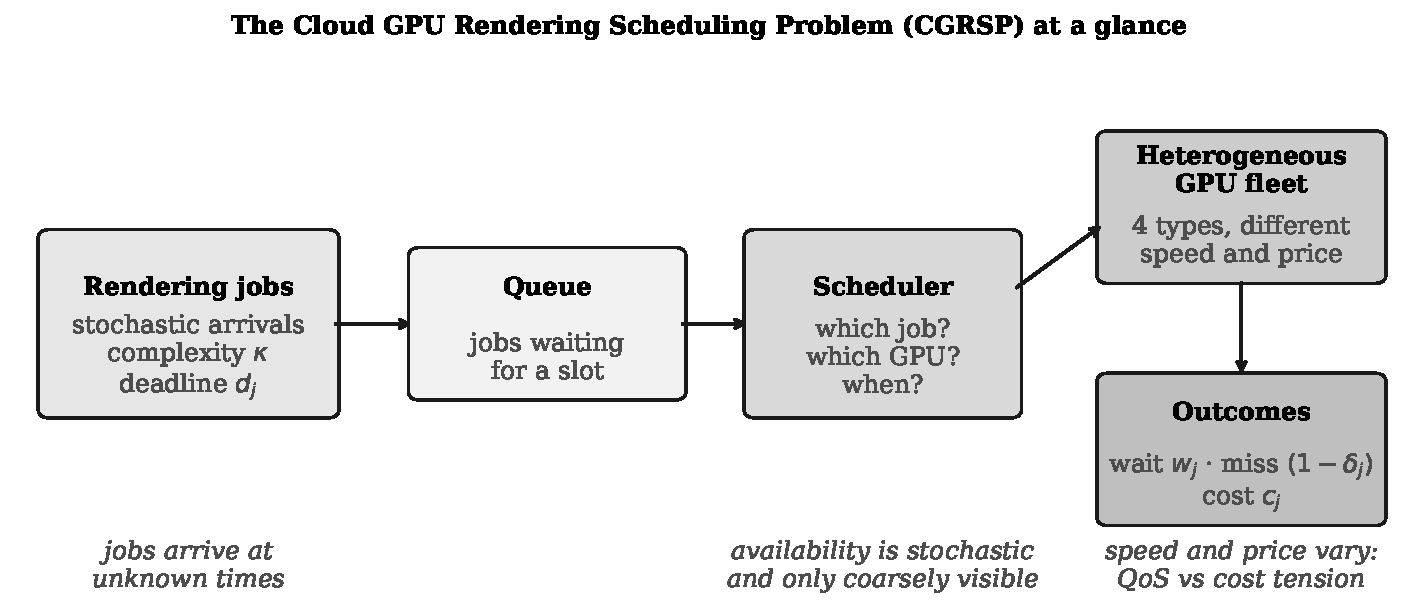
\includegraphics[width=0.97\textwidth]{figures/problem_overview.pdf}
\caption[The CGRSP problem at a glance]{The Cloud GPU Rendering Scheduling Problem at a glance. Rendering jobs with a complexity level and a deadline arrive stochastically and wait in a queue; the scheduler decides which job to place on which GPU and when; the heterogeneous fleet (four GPU types with different speeds and prices, and stochastic availability) executes the jobs; and per-job outcomes (waiting time, deadline adherence, cost) are the quantities the scheduler is judged on.}
\label{fig:problem-overview}
\end{figure}

The formulation is grounded in 6,234 real rendering jobs logged by the author's RunPod rendering pipeline (6,030 from its production Serverless endpoint, 203 tagged as development runs and one with no environment tag) and is evaluated through a discrete-event simulator calibrated to March 2026 RunPod pricing.

\section{Computational Complexity}
\label{sec:computational-complexity}

The offline version of CGRSP (where all $n$ jobs are known in advance) is a generalisation of the weighted job scheduling problem on parallel unrelated machines with deadlines, which is NP-hard in the strong sense~\cite{pinedo2016scheduling}. For the online version (jobs revealed at their arrival times), online deadline-constrained scheduling without preemption admits no general worst-case performance guarantee against the offline optimum; even on a single preemptive processor, deadline-driven scheduling is optimal only while the system is underloaded~\cite{liu1973scheduling,dertouzos1974control}, and under overload no online algorithm can guarantee more than one quarter of the value achievable with full knowledge of future arrivals~\cite{baruah1992competitiveness}. This intractability motivates the use of practical heuristic policies rather than exact optimisation. The heuristic policies are benchmarked in Chapter~\ref{chap:experiments} against a FIFO baseline, with a certified capacity bound and a clairvoyant relaxation as additional reference points, rather than against an intractable optimum; reinforcement learning is a natural future extension (Section~\ref{sec:limitations-and-future-research}) but is not evaluated in this study.

\section{Research Objective}
\label{sec:research-objective}

This study pursues four research objectives:

\begin{enumerate}

\item \textbf{Formal Problem Formulation.} Define CGRSP as a rigorous mathematical optimisation problem with explicit notation, decision variables, constraints, and a bi-objective function, enabling reproducible comparison with future work.

\item \textbf{Simulator Construction and Calibration.} Build a discrete-event simulator of an on-demand RunPod Secure Cloud fleet, including empirically measured GPU execution times, a stochastic availability model, Poisson job arrivals, and per-second cost tracking, with its service-time inputs calibrated to 6,234 real rendering jobs and its schedules checked by a constraint verifier.

\item \textbf{Comparative Evaluation of Scheduling Heuristics.} Implement and statistically compare ten scheduling algorithms: FIFO (baseline), Shortest Processing Time (SPT), Earliest Deadline First (EDF), Lowest Cost First (LCF), Balanced (weighted speed-cost composite), Random, SPT+Rescue (SPT with laxity-based deadline rescue), an adaptive queue-pressure EDF-SPT hybrid, the novel anticipative Rolling-Horizon (RH) scheduler, and the Cost-Aware Deadline-Risk (CADR) scheduler. Assess them across a four-phase evaluation programme: single-seed benchmark, 30-seed statistical validation, day-type and deadline-tightness sensitivity, and a 30-day monthly simulation whose day-type mix is taken from real RunPod billing data.

\item \textbf{Deployment Guidance.} Translate experimental findings into actionable recommendations, grounded in paired statistical tests, for cloud rendering operators: establish which of the two proposed schedulers should be the default and when the other is preferable (CADR as the default, since its paired baseline miss difference from RH is not significant (equivalence untested), it has close monthly miss point estimates with lower tardiness, and it leads under eased availability and the data-ordered per-type ranking; RH as the specialist for the scarce baseline availability regime when only the count of missed deadlines matters, and SPT for operators who prioritise queue wait), quantify when SPT's wait-time advantage outweighs its deadline risk, identify the tight-deadline fraction threshold at which EDF becomes preferable, and characterise the role of the concurrency limit $C_{\max}$ as the primary performance lever.

\end{enumerate}

\section{Research Contribution}
\label{sec:research-contribution}

The primary contributions of this study are:

\begin{itemize}

\item A complete mathematical formulation of CGRSP, including a three-state availability model (its unavailable state is retained for generality and does not occur on the on-demand platform studied), a bi-objective QoS-cost function, and all assignment and temporal constraints (Chapter~\ref{chap:formulation}).

\item A verified discrete-event simulator implemented in Python, calibrated against the full empirical rendering-job dataset (Chapter~\ref{chap:system}).

\item A statistically rigorous comparison of ten scheduling algorithms (eight benchmarks, including an adaptive EDF-SPT hybrid, plus the two proposed schedulers) on the saturated hectic-day configuration of Section~\ref{ssec:platform-and-data} ($n=30$ seeds, $\rho>1$), using paired $t$-tests, Cohen's $d$ effect sizes, and a Holm-Bonferroni correction. The comparison establishes SPT as the lowest-wait baseline (with no significant paired wait difference from RH), but significantly outperformed by EDF on miss, and quantifies the deadline penalty of the deadline-oblivious policies (Chapter~\ref{chap:experiments}).

\item A day-type sensitivity study (quiet/normal/hectic/surge, 30 seeds each) showing that the scheduler ranking is regime-dependent: RH has the lowest miss point estimate on hectic days (above saturation, $\rho>1$; no significant paired miss difference from CADR in the Phase~3 30-seed test), while the Adaptive hybrid, EDF, and RH form the lowest miss tier on below-saturation surge days (no paired test is computed for the day-type sweep) (Chapter~\ref{chap:experiments}).

\item A deadline-tightness sensitivity study under the surge-day configuration of Section~\ref{ssec:platform-and-data} (30 seeds per sweep point) locating the crossover between deadline-driven and shortest-job-first ordering: among the seven baseline policies in the sweep, EDF attains significantly lower miss than SPT when tight fraction $\leq 30\%$, the paired test does not resolve their difference at the midpoint of the sweep ($50\%$), and SPT attains significantly lower miss from $\geq 70\%$; no scheduler achieves 0\% misses across all fractions at surge-day load (Chapter~\ref{chap:experiments}).

\item A 30-day monthly operational simulation (Phase~4, 10 replications) whose mix of day types is taken from RunPod billing data (22~April to 21~May 2026), showing that RH and CADR remain the lowest-miss pair at monthly scale (near-identical, RH marginally lower, with no paired test at that phase), while RH's hectic-day wait advantage does not carry over, and identifying the concurrency budget $C_{\max}$ as the binding throughput constraint at the assumed hectic-day stress load (Chapter~\ref{chap:experiments}).

\item Two complementary deadline-aware schedulers: (i) the Rolling-Horizon (RH) scheduler, which at each event plans over the slot-availability timeline and anticipated arrivals, keeping shortest-processing-time ordering for jobs with slack, promoting only jobs the timeline shows would otherwise miss, and demoting jobs projected to miss under mean-service estimates to prioritise jobs projected to meet their deadlines; RH has the lowest deadline miss point estimate of the ten policies (no significant paired difference from CADR in Phase~3) with no significant paired wait difference from SPT, significantly outperforming SPT+Rescue on miss; and (ii) the Cost-Aware Deadline-Risk (CADR) scheduler, which classifies jobs by a scale-free critical ratio and selects the cheapest deadline-feasible node; CADR has a close miss point estimate to RH at substantially lower tardiness, has close monthly miss point estimates with lower tardiness, and leads under eased availability and the data-ordered per-type ranking, and also has a lower miss point estimate than SPT+Rescue (no pre-specified paired test), at essentially the same wait. The study recommends CADR as the default scheduler and RH as the specialist for the scarce baseline availability regime when only the miss count matters; operators who prioritise queue wait should use SPT (Chapter~\ref{chap:experiments}; see also Research Objective~4 above).

\end{itemize}

\section{Scope and Limitations}
\label{sec:scope-and-limitations}

This study focuses on scheduling 3D rendering workloads in a simulated on-demand GPU fleet modelled with RunPod Secure Cloud prices from March 2026. The evaluation is based on the empirical dataset of real rendering jobs collected between July 2025 and June 2026, spanning four GPU types (RTX~3090, RTX~A5000, RTX~A4000, RTX~A4500) and three scene complexity levels.

Several limitations bound the scope of this work. The baseline concurrency limit is five instances, RunPod's default per-account worker quota ($C_{\max}$, Section~\ref{ssec:platform-and-data}), which serves as the primary throughput constraint and is varied only in a dedicated sensitivity sweep. The hectic and surge workloads are stress loads above the busiest recorded day, and operating costs use RunPod Pods (Secure Cloud) prices although the job data came from a Serverless endpoint. The baseline availability probabilities are modelling assumptions rather than measured frequencies, since the author's pricing-API snapshots show the fleet types almost never at High stock and often with no Secure Cloud offer at all; a sensitivity sweep over the assumed baseline availability probabilities (Chapter~\ref{chap:experiments}) shows that the proposed and rescue-style deadline-aware policies stay ahead of the deadline-blind ones at every operable setting (plain EDF ties SPT at the scarcer $\times0.75$ setting), but the order within the leading pair is not stable: RH's miss lead over CADR is significant only at the scarcer operable setting, the most eased setting lets several policies reach zero misses while RH does not, and permuting the per-type ranking to the order the snapshot record's offer shares support moves the lead to CADR; the scarcest settings leave the fleet inoperable for every policy alike (Chapter~\ref{chap:conclusion}). The study also assumes non-preemptive scheduling, as CGRSP models each rendering frame as a single indivisible job and does not split a frame into pixels, samples, tiles or sub-frames; rendering one frame across multiple GPUs is not considered. A six-mix fleet-composition sweep at ten seeds is a sensitivity check on one workload, not a second studio trace, and the learned baseline in the comparison is a shallow tabular bandit rather than a deep policy, so its null result is not evidence about deep reinforcement learning. These limitations are discussed in detail, together with directions for future research, in Chapter~\ref{chap:conclusion}.

\section{Organisation of Thesis}
\label{sec:organisation-of-thesis}

The remainder of this thesis is organised as follows:

\textbf{Chapter~\ref{chap:related}} reviews related work on cloud GPU rental, classical and heterogeneity-aware scheduling, learning-based and LLM-assisted scheduling, anticipatory reservation, discrete-event simulation and statistical evaluation, and 3D rendering workloads, motivating this study's design choices.

\textbf{Chapter~\ref{chap:formulation}} presents the formal CGRSP formulation: notation tables, an informal system and state description, a unified model (the lexicographic objective, assignment constraints, stochastic availability, and temporal/QoS constraints), and a numerical example.

\textbf{Chapter~\ref{chap:system}} describes the system architecture: the discrete-event simulator core, the RunPod fleet model, the job generator, and the implementations of all ten scheduling algorithms.

\textbf{Chapter~\ref{chap:experiments}} presents the full experimental evaluation: the seven-scheduler Phase~2 hectic-day benchmark (the seven baseline policies; RH, CADR and the Adaptive hybrid enter in Phase~3), Phase~3 statistical analysis over 30 seeds with an ablation tracing the design chain (FIFO $\to$ SPT $\to$ SPT+Rescue $\to$ RH, plus CADR and the CADR-order-only ablation), sensitivity analyses for the critical-ratio threshold, anticipation reservation, concurrency limit ($C_{\max} \in \{3,5,7,8,10\}$), rescue threshold, queue-pressure threshold and objective weights, a capacity lower bound, day-type and deadline-tightness sensitivity, a tardiness-objective robustness study, robustness checks (availability model, estimated cells, label noise and GPU speed), and Phase~4 monthly operational simulation.

\textbf{Chapter~\ref{chap:conclusion}} concludes the study with a discussion of theoretical implications, practical deployment guidance, limitations, and directions for future research.

\chapter[Background and Related Work]{\texorpdfstring{Background and\\Related Work}{Background and Related Work}}
\label{chap:related}

\section{Cloud GPU Computing}
\label{sec:cloud-gpu-computing}

General-purpose computation on graphics hardware became practical with NVIDIA's CUDA platform~\cite{nickolls2008scalable}, and GPU computing was subsequently offered as a cloud service. Early cloud providers (AWS, Azure, GCP) offered GPU instances as part of virtual machine (VM) rental services, billed hourly with a minimum session length of a full hour on AWS~\cite{barr2017persecond}. The rise of deep learning as a primary GPU workload in the 2010s drove rapid expansion of GPU instance types and the emergence of spot-pricing markets where unused capacity is offered at discounted rates with potential preemption~\cite{yi2010reducing,subramanya2015spoton,zheng2015bid}.

By the early 2020s, a second tier of GPU cloud providers, such as RunPod, Lambda, CoreWeave, and Vast.ai, had emerged, some with billing granularity as fine as one second~\cite{runpod2026podspricing,vastai2026concepts}. Marketplace-style platforms such as RunPod and Vast.ai aggregate GPU hardware from data-centre operators and individual hosts~\cite{runpod2026podsoverview,vastai2026concepts}, and these providers collectively offer a heterogeneous catalogue of GPU types~\cite{runpod2026podspricing,coreweave2026pricing,lambda2026pricing} (consumer-grade RTX series, workstation-grade A-series, data-centre A100/H100) at widely varying price points. For rendering workloads, which tend to be short (tens of seconds to a few minutes per frame) and embarrassingly parallel at the frame level, per-second billing and the ability to spin up many low-cost nodes simultaneously make these platforms attractive alternatives to dedicated render farms.

The key distinguishing feature of on-demand cloud GPU rental relevant to this thesis is \emph{qualitative availability}. Unlike reserved VM instances with guaranteed exclusive access and pre-provisioned capacity, an on-demand instance must be acquired afresh from a pool whose stock fluctuates with competing demand: when stock is scarce, acquiring an instance of a given type incurs a provisioning delay. From the perspective of the scheduling algorithm, this manifests as a coarsened observable state: the platform API exposes a qualitative per-type stock status, but not the underlying cause (customer demand, maintenance, hardware fault). This is the abstraction encoded in the CGRSP stochastic availability model, which targets the RunPod Secure Cloud on-demand model (where a running instance is not reclaimed) rather than spot preemption.

A critical distinction separating marketplace GPU rental from the managed-cluster context of most scheduling literature is rarely made explicit. \textbf{Reserved-cluster schedulers}, including HEFT~\cite{topcuoglu2002heft}, Gavel~\cite{narayanan2020gavel}, and Optimus~\cite{peng2018optimus}, operate on machine or GPU pools under the operator's exclusive control; node availability is guaranteed and the scheduling problem reduces to job-to-node assignment. \textbf{Marketplace scheduling}, by contrast, must treat GPU availability as externally determined: competing customer demand, platform maintenance windows, and hardware failures collectively determine which GPU types can be provisioned at any given moment, outside the operator's control. This distinction is structural, not incidental: the scheduler must treat availability as a stochastic first-class input rather than a deterministic constraint. This is precisely the gap the CGRSP formulation closes. A third body of work, \textbf{spot and transient-instance scheduling}, does treat cloud availability as stochastic, but models it as mid-job \emph{revocation} risk: checkpointing against instance loss~\cite{yi2010reducing}, batch services that absorb revocations~\cite{subramanya2015spoton}, and bidding strategies over spot price processes~\cite{zheng2015bid}. The on-demand Secure Cloud setting of this thesis is structurally different: a held instance is never reclaimed, so no checkpoint or migration machinery is relevant, and scarcity manifests instead as a stochastic provisioning delay at acquisition time, observed only as a coarse per-type stock status inside every dispatch decision. That acquisition-side availability problem is the one the surveyed spot literature does not address.

Recent work has moved closer to the marketplace setting without reaching it. SkyNomad~\cite{li2026skynomad} schedules deadline-bound GPU batch jobs across spot instances in several cloud regions, probing whether spot capacity can currently be obtained in each region and predicting how long an instance will survive before preemption, but it treats availability as a binary per-region signal backed by an always-available on-demand fallback, makes decisions for a single job rather than dispatching a queue of jobs, and treats the deadline as a hard guarantee under a cost-minimising objective. REACH~\cite{yu2025reach} targets community GPU platforms that aggregate peer-contributed consumer GPUs, the topology closest to a GPU marketplace, but it models the volatile reliability of nodes during execution with a learned transformer-based policy rather than scarcity at acquisition time. BOA Constrictor~\cite{li2026boa} takes the renter's side of cloud GPU rental, deciding how many GPUs of each priced type to rent under a long-run budget, yet it assumes rented capacity is always obtainable and optimises mean job completion time with no deadlines. None of the three observes availability as a coarse stock status at dispatch time, which is the setting CGRSP formalises.

\section{Classical Job Scheduling}
\label{sec:classical-job-scheduling}

Job scheduling on a set of machines to minimise one or more performance criteria is one of the most well-studied topics in operations research and computer science~\cite{pinedo2016scheduling}. Graham et al.~\cite{graham1979optimization} established the three-field notation $\alpha|\beta|\gamma$ for scheduling problems. For CGRSP, the problem is closest to $P_m|\text{online}, r_j, d_j|\sum \omega_j C_j$ (parallel identical machines with online arrivals, release times, deadlines, and weighted completion time; the weight is written $\omega_j$ here to avoid a clash with the waiting time $w_j$), except that the machines in CGRSP are not identical: they differ in speed and cost, and their speed ranking depends on the job, making it a generalisation to unrelated parallel machines ($R_m$) rather than uniform parallel machines ($Q_m$). A uniform-machine model would require one speed factor per machine that applies to every job, and the fleet violates this, because the stratum means rank the types differently across complexity levels: at $\kappa=1$ the RTX~3090 (59.5\,s) edges the RTX~A5000 (60.7\,s), at $\kappa=2$ the A5000 (69.1\,s) edges the 3090 (69.6\,s), and at $\kappa=3$ the RTX~A4500 is fastest (88.3\,s), followed by the 3090 (91.2\,s), the A5000 (94.5\,s) and the A4000 (98.6\,s) (Table~\ref{tab:gpu_specs}). The $\kappa=1$ cells for the A4000 and A4500, and the sparse $\kappa=2$ A4000 cell, are model estimates rather than measurements (Section~\ref{sec:gpu-fleet-model}), and these are observational stratum means rather than scene-matched comparisons, so the ranking is a property of the workload mix as much as of the hardware.

\subsection{Shortest Processing Time (SPT)}
\label{ssec:shortest-processing-time-spt}

The Shortest Processing Time rule assigns the available processor to the ready job with the smallest processing time. Smith~\cite{smith1956various} proved that ordering jobs by processing time divided by weight (WSPT) minimises total weighted completion time on a single machine; with equal weights this reduces to SPT, which therefore minimises average completion time. On identical parallel machines, SPT list scheduling (assigning the shortest unscheduled job to whichever machine becomes free next) remains optimal for minimising total completion time, and hence average flow time, in the offline setting with all jobs available at time zero~\cite{pinedo2016scheduling}. In online settings with Poisson arrivals, SPT minimises mean response time among non-preemptive policies (a classical result from M/G/1 queueing theory~\cite{pinedo2016scheduling}). SPT's weakness in deadline-constrained settings is its tendency to starve large, long-running jobs: a steady stream of short jobs keeps a machine busy and can delay deadline-critical long jobs past their deadlines.

\subsection{Earliest Deadline First (EDF)}
\label{ssec:earliest-deadline-first-edf}

Earliest Deadline First, attributed to Jackson~\cite{jackson1955scheduling}, whose deadline ordering Lawler and Moore~\cite{lawler1969functional} later built into an exact dynamic-programming method for the weighted number of tardy jobs, prioritises the ready job with the nearest deadline. EDF is optimal on a single preemptive machine in the feasibility sense: if any policy can meet every deadline, EDF does~\cite{dertouzos1974control}; Liu and Layland~\cite{liu1973scheduling} established the corresponding 100\% utilisation bound for periodic task sets. On non-preemptive parallel machines, the setting of CGRSP, EDF does not provide a worst-case guarantee for deadline violation minimisation. The Phase~3 deadline sensitivity experiments in Chapter~\ref{chap:experiments} instead separate its comparison against shortest-job-first ordering (SPT) into three regimes: EDF attains significantly lower miss when the tight-deadline fraction is low ($\leq 30\%$; at $30\%$, $t=\DlThirtySPTEDFmissT$, $\DlThirtySPTEDFmissP$), the paired test does not resolve their difference at the midpoint of the sweep ($50\%$, $t=\DlFiftySPTEDFmissT$, $\DlFiftySPTEDFmissP$), and SPT attains significantly lower miss at high tight fractions ($\geq 70\%$; at $70\%$, $t=\DlSeventySPTEDFmissT$, $\DlSeventySPTEDFmissP$).

\subsection{First-In-First-Out (FIFO)}
\label{ssec:first-in-first-out-fifo}

FIFO processes jobs in the order they arrive. It provides fairness guarantees (no starvation), requires no knowledge of processing time or deadline, and has long served as the default scheduling policy in batch computing systems, dating to the earliest resident-monitor mainframe operating systems~\cite{silberschatz2018operating}. FIFO is used as the primary baseline in this study because it represents the ``do nothing special'' approach. In the M/M/c queueing model, FIFO achieves the same throughput as any work-conserving policy (by work-conservation arguments~\cite{pinedo2016scheduling}), but it does not minimise mean response time or deadline adherence.

\subsection{Other Heuristics}
\label{ssec:other-heuristics}

\textbf{Lowest Cost First (LCF)} prioritises the GPU type with the lowest effective rental cost per job, defined as the product of the rental rate and the expected execution time: $\text{cost}_{\text{eff}}(j, m) = p_{g(m)} \cdot \mathbb{E}[W(\kappa_j, g(m))]$. LCF is motivated by cost-minimisation objectives, relevant for rendering studios operating under tight production budgets where deadline pressure is low. A complicating factor is GPU availability reliability: a ``cheap'' GPU type with consistently low stock may increase effective turnaround through long provisioning delays. This is addressed in the CGRSP implementation through a proportional stock-status penalty added to the effective cost.

\textbf{Balanced scheduling} combines processing speed (SPT-like) and cost (LCF-like) criteria through a weighted composite score. A weight $w_b \in [0, 1]$ controls the trade-off: $w_b \to 1$ approaches SPT behaviour (speed priority), $w_b \to 0$ approaches LCF (cost priority). In the CGRSP implementation, $w_b = 0.8$ (speed-biased) is used, with global-max normalisation to prevent one criterion from dominating due to differing numerical scales. (The weight is written $w_b$ to avoid a clash with the objective weights $\alpha_1, \alpha_2$ of Chapter~\ref{chap:formulation}.) Unlike EDF and SPT, Balanced does not reorder jobs; it sorts only on node selection, maintaining FIFO job ordering. This design choice ensures that Balanced is statistically distinguishable from both EDF (which reorders by deadline) and SPT (which reorders by processing time) in the comparative evaluation.

\section{Heterogeneous Machine Scheduling}
\label{sec:heterogeneous-machine-scheduling}

When machines have different speeds, the scheduling problem becomes significantly harder. Braun et al.~\cite{braun2001comparison} provided the first systematic comparison of scheduling heuristics on heterogeneous machines, evaluating 11 algorithms including min-min, max-min, genetic algorithms, and simulated annealing in terms of makespan. Their study on synthetic workloads found that the relatively simple min-min heuristic, which repeatedly selects, among all unmapped tasks, the one with the smallest earliest-completion time and assigns it to that machine, performs well in comparison with far more complex search methods, although the genetic algorithm produced the best mappings overall. CGRSP's SPT policy (Chapter~\ref{chap:system}) resembles a single-pass form of min-min restricted to the currently idle nodes: at each scheduling event it orders the queued jobs by their best expected execution time over the idle nodes, which equals the earliest completion time min-min selects on only when the stock-dependent provisioning delay that every CGRSP dispatch incurs (Chapter~\ref{chap:formulation}) is set aside or stock is uniform across the idle nodes; it also computes that ordering once per event rather than after every assignment. It then places each job using a composite of speed, cost, and stock status, which reduces to the minimum-completion-time (MCT) machine choice of the same study only when cost and stock are uniform across the idle nodes.

The Heterogeneous Earliest Finish Time (HEFT) algorithm of Topcuoglu et al.~\cite{topcuoglu2002heft} is the most widely cited heuristic for scheduling task-dependency DAGs on heterogeneous parallel machines. HEFT ranks tasks by upward rank (estimated time to completion including successors) and assigns each task to the machine that minimises its finish time. For CGRSP, jobs are independent (no DAG dependencies), so each job's upward rank collapses to its mean execution time across machine types, and HEFT reduces to longest-average-job-first ordering with earliest-finish-time machine selection. It therefore orders jobs in the reverse of the SPT policy described in Chapter~\ref{chap:system}, and, unlike HEFT, SPT selects nodes by a composite of speed, cost, and stock status rather than by earliest finish time alone.

GPU program schedulers operate at a finer granularity. Chien et al.~\cite{chien2018graph} represent an OpenCL program as a computational graph of kernels with their metadata and dependencies, then schedule kernel tasks across heterogeneous CPU and GPU devices, using code analysis to choose the target device and work-group size. Chang et al.~\cite{chang2020dependent} develop a framework for dependent GPU programs, where kernel ordering is considered together with memory write-back policy to avoid unnecessary data movement. Both operate within a single node and optimise execution performance; the decisions are kernel order, device choice and memory policy, not which rented node receives which job. CGRSP treats each rendering frame as one indivisible, non-preemptive job (Section~\ref{sec:3d-rendering-workloads}), so these decisions lie outside its model, and decomposing frames into dependent passes would need both layers.

More recent work targets deep learning workloads on GPU clusters specifically. Ye et al.~\cite{ye2024deep} surveyed deep learning workload scheduling in GPU data centres, cataloguing approaches ranging from static profiling-based assignment to online reinforcement learning-based policies. Peng et al.~\cite{peng2018optimus} proposed Optimus, a performance model-driven scheduler for deep learning jobs that reduces training time by dynamically adjusting resource allocation. These approaches differ from CGRSP in that they focus on \emph{training} jobs (which can be checkpointed and migrated) rather than batch rendering jobs (which are typically non-preemptive and short).

Narayanan et al.~\cite{narayanan2020gavel} proposed Gavel, a heterogeneity-aware cluster scheduler for deep learning workloads that expresses scheduling policies (fairness, FIFO, makespan, cost, finish-time fairness, among others) as optimisation problems over per-GPU-type time allocations, realised by a round-based priority mechanism. Gavel explicitly models the performance differential across heterogeneous GPU types and demonstrates that heterogeneity-aware scheduling substantially reduces average job completion time compared to homogeneous-assumption baselines, a result conceptually aligned with CGRSP's finding that SPT's wait-time advantage depends on exploiting per-complexity GPU performance differences. Gavel, however, treats the number of workers of each GPU type as a fixed, known capacity, even in its public-cloud cost policies, is evaluated on long-running training jobs (hours, checkpointable), and supports deadlines only as per-model throughput SLO constraints within its cost-minimisation policy. CGRSP differs on all three dimensions: stochastic on-demand availability with provisioning delay, short non-preemptive rendering frames, and mixed tight/loose deadline constraints.

Two more recent results reinforce the same point from different angles. Sia~\cite{jayaramsubramanya2023sia} extends heterogeneity-aware scheduling to elastic training jobs, choosing both the GPU type and the GPU count for each job to maximise cluster goodput, and reports gains over Gavel; like Gavel, it assumes a dedicated cluster, and it has no notion of per-job deadlines. M\'elange~\cite{griggs2024melange} shows for large language model serving that GPU cost efficiency does not track price: the cheapest GPU type per unit of work depends on the request profile, so a mixed fleet can undercut any single type. This mirrors the non-monotone speed and price ranking of the CGRSP fleet (Figure~\ref{fig:gpu-heatmap}), although M\'elange solves an offline fleet-sizing problem rather than online dispatch.

\section{Reinforcement Learning for Scheduling}
\label{sec:reinforcement-learning-for-scheduling}

The application of reinforcement learning (RL) to scheduling and resource management has received substantial attention since the seminal work of Mao et al.~\cite{mao2016resource}, who trained a neural-network policy with a variant of REINFORCE to schedule jobs whose multi-resource demands and durations are known on arrival onto a cluster treated as a single resource pool, performing comparably to or better than Shortest-Job-First and a Tetris-inspired packing heuristic on average job slowdown. Their formulation (an image-based state encoding cluster occupancy and the resource profiles of waiting jobs, and a small discrete action space of $M$ visible job slots plus a no-op) is conceptually related to meta-scheduler approaches for cloud GPU scheduling.

Subsequent work applied deep Q-networks (DQN)~\cite{mnih2015human} to various scheduling domains. Chen and Chen~\cite{chen2023gpu} proposed DeepGJS, which compares policy-gradient, DQN and Double-DQN agents for allocating GPU jobs to servers, with the aim of minimising slowdown and completion time; they report that it outperforms shortest-job-first, Packer and DeepRM baselines. Like other deep-RL schedulers, it must be trained on simulated workloads before deployment, a training cost that the heuristic-only approach pursued in this thesis avoids.

Zhou et al.~\cite{zhou2024deep} surveyed deep RL methods for cloud resource scheduling, identifying three main challenges: (1) large state-action spaces requiring function approximation, (2) sparse and delayed rewards, and (3) non-stationarity from competing workloads. These challenges motivate the heuristic-based approach in CGRSP, where domain knowledge is encoded directly into the scheduling rules rather than learned from scratch.

A newer line of work brings large language models (LLMs) into scheduling. Krishnamurthy and Shiva~\cite{krishnamurthy2025llmsarsa} use an LLM to supply heuristic value estimates that guide a SARSA agent for dynamic cloud task scheduling, evaluated in the CloudSim Express simulator, assigning tasks to virtual machines, on workloads drawn from a Google cluster dataset. Other work uses LLMs to design heuristics rather than to act as the scheduler: ReEvo~\cite{ye2024reevo} evolves heuristic code for combinatorial optimisation problems using LLM-generated reflections, and {\c{C}}etinkaya et al.~\cite{cetinkaya2025discovering} use an LLM to discover heuristics for single-machine total tardiness scheduling inspired by the classical earliest-due-date and modified-due-date rules. The last of these builds on the same due-date lineage (Section~\ref{ssec:earliest-deadline-first-edf}) as the EDF-based policies evaluated in this thesis. CGRSP does not use LLMs; its policies are hand-designed and interpretable, but LLM-driven heuristic discovery is a plausible route to extending them (Section~\ref{ssec:future-research}).

\section{Anticipatory and Proactive Scheduling}
\label{sec:anticipatory-and-proactive-scheduling}

The Rolling-Horizon (RH) scheduler introduced in this thesis holds idle capacity for tight-deadline jobs expected to arrive shortly, instead of reacting only once they arrive. The closest precedent is the anticipatory scheduler of Chugh et al.~\cite{chugh2023anticipatory}. In a public cloud's machine-learning training service, where users hold dedicated GPU pools, it lends idle GPUs from one pool to jobs from other pools only when coarse forecasts of each pool's future load and of job durations indicate that the donor pool's own later jobs will not be slowed. It is designed to be robust to prediction errors that do not follow simple error models, and on production workloads it reduces average job latency by 2.83$\times$ relative to the production scheduler. Parcae~\cite{duan2024parcae} applies proactive reasoning to spot instances, predicting upcoming preemptions and reconfiguring a training job's parallelism before they occur, and GFS~\cite{duan2026gfs} uses per-tenant demand forecasts to size a spot quota inside a large production GPU cluster, protecting high-priority service-level objectives while limiting evictions of low-priority work. All three show that acting on a forecast before the event can outperform purely reactive allocation, which supports the design premise of RH. They also differ from CGRSP. Chugh et al. and GFS operate inside clusters their operator owns. Parcae does use rented spot capacity, but it adapts one running training job to preemptions rather than scheduling a queue of independent jobs. None models acquisition-time provisioning delay under a qualitative stock status, and none evaluates its proactive policy against a mix of tight and loose per-job deadlines. RH also gates its reservation on offered load, disabling it under saturation, a safeguard none of the three needs because none reserves capacity against deadline risk.

\section{Discrete-Event Simulation}
\label{sec:discrete-event-simulation}

Discrete-event simulation (DES) models the evolution of a system through a chronologically ordered sequence of events, each of which can modify system state and schedule future events~\cite{banks2010discrete}. DES is the standard methodology for evaluating scheduling algorithms when analytical queueing models are intractable, as is the case for heterogeneous machines with general service time distributions.

The CGRSP simulator adapts the event-driven core of SPARS~\cite{amrizal2026spars}, an HPC job-scheduling simulator; its node power-state manager and energy metrics are replaced by the cloud GPU fleet and QoS/cost metrics of Chapter~\ref{chap:system}.

Sargent~\cite{sargent2013verification} sets out the verification and validation (V\&V) framework for simulation models that this thesis follows: (1) conceptual model validity (does the model represent the real system?), (2) computerized model verification (is the model implemented correctly?), (3) operational validity (do simulation outputs match real system outputs?), and (4) data validity (are model inputs accurate?). Of these four, the CGRSP simulator has been partly checked for data validity, which Sargent notes is often not counted as part of model validation proper: its service-time inputs are log-normal distributions whose per-stratum means and log-space dispersions are fitted to the measured execution times of the 6,234-job empirical dataset, whereas its hectic and surge job counts and its availability probabilities are stated modelling assumptions (Section~\ref{ssec:platform-and-data}) and its prices are RunPod Pods rates rather than the Serverless rates of the production pipeline (Table~\ref{tab:gpu_specs}). Computerized model verification is partial: a constraint verifier (Section~\ref{sec:metrics-collection}) re-checks deadline flags, the miss count and per-job costs against the recorded per-job data, and single dispatch and one-job-per-node occupancy (from dispatch to completion) against a complete dispatch log, for all ten policies, but only on the single seed-42 hectic-day workload. No conceptual-model or operational validation has been performed; operational validation against live platform outputs is left to future work (Section~\ref{ssec:future-research}).

Law and Kelton~\cite{law2000simulation} identified statistical output analysis, including confidence intervals, variance reduction techniques, and sensitivity analysis, as essential for credible simulation results. This thesis follows these recommendations: every inferential claim rests on multiple independent replications (seeds), the single-seed Phase~2 benchmark and the single-replication Phase~4 timeline figure being illustrative only, and 95\% confidence intervals are reported for Phase~3 statistical results.

The statistical reporting also follows more recent guidance specific to computer systems evaluation. Kalibera and Jones~\cite{kalibera2020quantifying} found that a majority of the systems papers they surveyed quantified performance changes as bare ratios of execution time, almost never with their uncertainty, and argued for effect-size confidence intervals instead. Krishnamachari~\cite{krishnamachari2026statistical} sets out a minimum defensible evaluation for engineering and computer science papers (among its items: multiple independent seeds, paired comparisons, effect sizes with 95\% confidence intervals, and validation of the simulator), separately recommends multiple-comparison correction when many tests are reported, and uses a comparison of job-scheduling policies on simulated workloads as its running example. On the statistical side, the Phase~3 design follows these recommendations: paired replications across 30 seeds, Holm-corrected tests~\cite{holm1979simple}, and Cohen's $d$~\cite{cohen1988statistical} for every comparison in the pairwise family, and, for each pre-specified comparison printed in the Phase~3 $t$-test table, the paired mean difference with its 95\% confidence interval (Section~\ref{ssec:statistical-methodology}); supplementary tests quoted elsewhere, such as the RH-versus-SPT wait tie and the deadline-sweep comparisons, are given with $t$ and $p$ only. The simulator-validation item is only partly met: the model's service-time inputs are checked against the empirical dataset and part of its implementation is checked by a constraint verifier, but its outputs have not been validated against the live platform.

\section{3D Rendering Workloads}
\label{sec:3d-rendering-workloads}

Three-dimensional (3D) rendering is the process of computing the colour of each pixel in an image from a geometric scene description, camera model, and light sources. Path tracing~\cite{pharr2023physically}, the algorithm used by most modern renderers (Cycles in Blender, V-Ray, Arnold), is embarrassingly parallel at the pixel level: each pixel's colour is estimated independently by tracing thousands of random light paths. Pixel-level parallelism is a property of the renderer, not of the scheduling unit: this thesis schedules at the granularity of the frame, so one job is one complete rendered image, whether a still or a frame of an animation, and not a pixel, a sample, a tile, a sub-frame or a group of frames. A frame can be rendered on a single GPU without inter-node communication, so a job needs exactly one node.

Rendering job duration depends primarily on scene complexity (polygon count, light count, material complexity), image resolution, and the number of samples per pixel~\cite{pharr2023physically}. In this thesis, job complexity is abstracted to three levels ($\kappa \in \{1, 2, 3\}$), with per-stratum log-normal execution times whose means are derived from the 6,234-job dataset. The dataset spans a wide range of complexities: high-complexity jobs take roughly 64\% to 69\% longer than low-complexity jobs on the two GPU types with measured low-complexity jobs (the RTX~A5000 and RTX~3090; per-stratum means in Table~\ref{tab:gpu_specs}). The A4500 and A4000 have no low-complexity jobs in the dataset, so their low-complexity means are estimates. This heterogeneity in job duration is precisely what makes SPT effective: by front-loading short jobs, it reduces the average number of jobs waiting in the queue.

The scheduling literature specific to render farms is small. RenderSelect~\cite{ruby2016renderselect} addresses cloud rendering at the level of choosing a provider, ranking competing services on cost and quality-of-service criteria rather than dispatching individual jobs. Zhu et al.~\cite{zhu2026collaborative} schedule distributed Blender rendering and generative subtasks on a fixed eight-node cloud testbed, where each free worker takes the queued subtask with the highest weighted score of priority, estimated runtime and data-transfer cost, benchmarking against FIFO, HEFT and OpenCue. Yang et al.~\cite{yang2026adaptive} predict the compute demand of animation rendering tasks with a learned model and assign them across three GPU architectures to reduce latency and energy use. None of these considers rented capacity with uncertain availability, per-job deadlines and rental cost together, the combination CGRSP addresses.

The four GPU types (RTX~3090, A5000, A4000, A4500) represent the consumer and prosumer tiers on marketplace platforms in early 2026. They span a factor of $\sim$1.8 in price and a speed spread of about 4\% at low and medium complexity and 14\% at high complexity (Table~\ref{tab:gpu_specs}; pooled averages reflect the workload mix). Figure~\ref{fig:gpu-heatmap} shows that speed is non-monotone across complexity levels and price does not track it, so neither dimension alone determines the best assignment.

\begin{landscape}
\begin{figure}[H]
\centering
\captionsetup{font=small,skip=6pt}
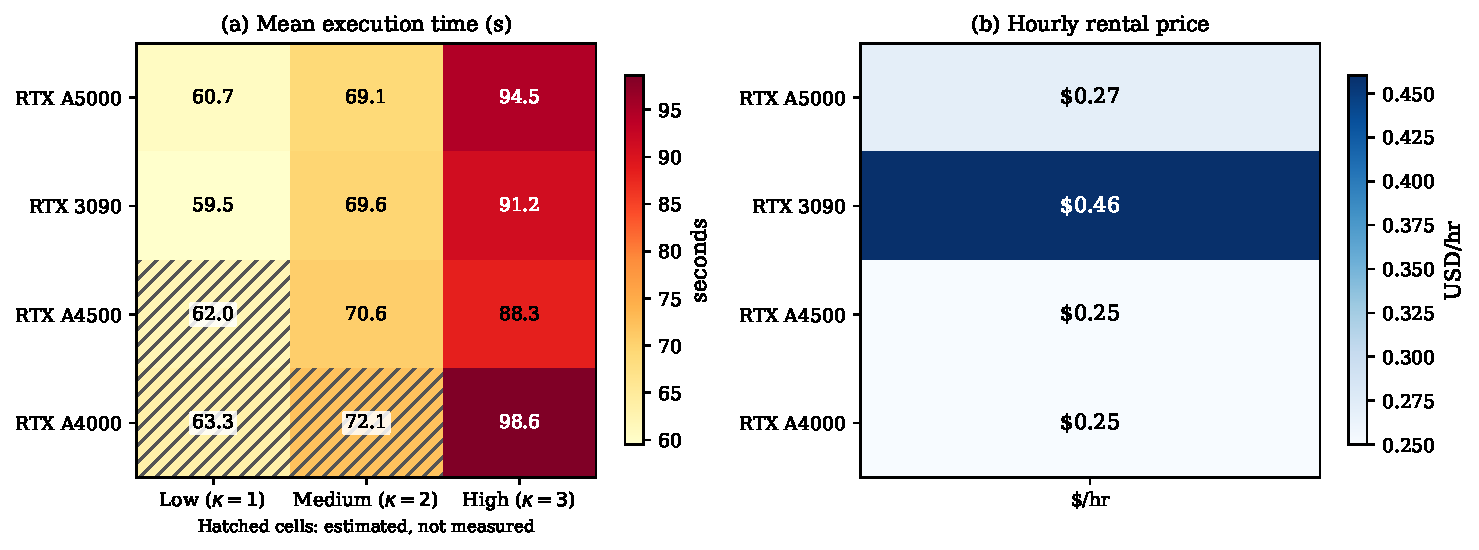
\includegraphics[width=0.98\linewidth,height=0.72\textheight,keepaspectratio]{figures/gpu_heatmap.pdf}
\caption[GPU fleet execution-time heterogeneity and pricing]{GPU fleet heterogeneity. Panel~(a): mean execution time (seconds) per GPU type and scene complexity level $\kappa$; the three model-estimated cells (low-complexity A4500 and A4000, medium-complexity A4000) are marked. The RTX~A4500 is fastest at high complexity (88.3\,s) despite having fewer CUDA cores than the RTX~3090 (91.2\,s), illustrating that the GPU speed ranking is non-monotone with respect to hardware specifications. Panel~(b): hourly rental price. The RTX~3090 is the most expensive (\$0.46/hr) yet has the lowest unweighted mean over the three complexity levels (73.4\,s, against 73.6\,s for the A4500 and 74.8\,s for the A5000, with three estimated cells included) and is second only to the A4500 at high complexity among the dense strata; the A4500 and A4000 share the same price (\$0.25/hr) while differing in speed, making node selection a genuine multi-criteria optimisation.}
\label{fig:gpu-heatmap}
\end{figure}
\end{landscape}

\section{Summary}
\label{sec:summary}

Table~\ref{tab:related_comparison} summarises the positioning of CGRSP relative to closely related work. Among the studies surveyed, CGRSP combines all four features the table compares: (1) real-world calibrated GPU heterogeneity, (2) stochastic qualitative availability (marketplace-driven, observed only as coarse stock status), (3) explicit deadline constraints, and (4) statistical evaluation across multiple seeds, day types, and concurrency limits. The table covers the foundational and GPU-scheduling studies; the three nearest recent works discussed above (SkyNomad, REACH, BOA Constrictor) are contrasted in the text rather than tabulated, and none of them observes availability as a coarse stock status. The per-second billing model is a property of the platform being modelled, not a compared dimension.

\begin{table}[htbp]
\centering
\small
\caption[Positioning of CGRSP against related work]{Positioning of CGRSP against related scheduling studies}
\label{tab:related_comparison}
\begin{tabular}{lcccc}
\toprule
\textbf{Work} & \textbf{GPU Hetero.} & \textbf{Stoch.\ Avail.} & \textbf{Deadlines} & \textbf{Stat.\ Valid.} \\
\midrule
Braun et al.~\cite{braun2001comparison} & Synthetic & \texttimes & \texttimes & \texttimes \\
HEFT~\cite{topcuoglu2002heft}           & Synthetic       & \texttimes & \texttimes & \texttimes \\
Mao et al.~\cite{mao2016resource}       & \texttimes & \texttimes & \texttimes & \checkmark \\
Chen \& Chen~\cite{chen2023gpu}             & Yes       & \texttimes & \texttimes & Limited \\
Ye et al.~\cite{ye2024deep}           & Yes (survey) & \texttimes & Partial   & \texttimes \\
Narayanan et al.~\cite{narayanan2020gavel} (Gavel) & Yes & \texttimes & Partial & \checkmark \\
\textbf{CGRSP (this thesis)}            & \checkmark & \checkmark & \checkmark & \checkmark \\
\bottomrule
\end{tabular}
\end{table}

Beyond the four dimensions in Table~\ref{tab:related_comparison}, CGRSP is, to the best of the author's knowledge, the first scheduling study of marketplace cloud GPU rental applied specifically to \emph{batch 3D rendering workloads}. Compared to deep learning training, the dominant focus of GPU scheduling literature~\cite{ye2024deep,peng2018optimus,narayanan2020gavel}, rendering frames have three properties that shape the scheduling design. First, execution is \emph{short and non-preemptive}: individual frames complete in tens of seconds to a few minutes, making checkpoint-and-resume impractical and favouring simple online dispatch policies over the long-horizon optimisation that DL training schedulers can exploit. Second, \emph{complexity is observable at submission}: scene complexity level ($\kappa$) is treated as known when a job enters the queue (in deployment it would be classified from scene statistics such as polygon and light counts that are available before rendering; in the calibration dataset it is proxied by render-time terciles, Section~\ref{ssec:platform-and-data}), providing the execution-time estimate that SPT and SPT+Rescue rely on. Third, \emph{GPU performance is non-monotone across complexity levels}: for high-complexity frames ($\kappa=3$), the RTX~A4500 (7,168 CUDA cores, 88.3\,s) has a lower observational stratum mean than the RTX~3090 (10,496 cores, 91.2\,s; see Table~\ref{tab:gpu_specs}), while at medium complexity the A5000 (69.1\,s) edges the 3090 (69.6\,s); these are not scene-matched evidence (Section~\ref{sec:gpu-fleet-model}), but they illustrate why the model uses per-complexity stratum means rather than a fixed GPU speed ranking. These three rendering properties shape the CGRSP formulation and calibration methodology.

\chapter{Problem Formulation and Mathematical Model}
\label{chap:formulation}

This chapter presents the mathematical formulation of the Cloud GPU Rendering Scheduling Problem (CGRSP). The problem models an on-demand GPU cloud where rendering jobs arrive continuously and must be scheduled to balance quality of service (QoS) and per-second operational costs. The formulation addresses three key challenges: (1) heterogeneous GPU types with varying performance and per-second rental rates, (2) stochastic provisioning delays driven by fluctuating market scarcity for each GPU type, and (3) temporal deadline constraints ensuring timely job completion.

The system operates as an on-demand GPU pool with $|\calN|$ nodes across $|\calG|$ resource types, serving a stream of rendering jobs with heterogeneous complexity levels. A job is one frame, that is, one complete rendered image, and it is scheduled as a single indivisible unit: a frame is not split into pixels, samples, tiles or sub-frames, and several frames are not combined into one job. Each job is assigned to exactly one node over the complete service horizon; a GPU instance of the node's type is provisioned for the duration of the job and billed per second of execution. The scheduler pursues a bi-objective criterion: minimising QoS penalties (waiting time and deadline violations) as the primary criterion while treating per-second operational cost as a secondary, tiebreaking criterion, subject to node availability and assignment constraints.

Occupancy and billing are deliberately modelled as two independent axes. On the occupancy axis, a node behaves as a persistent, single-tenant slot: once acquired it is held exclusively by one job for that job's full duration and is not shared, preempted, or reclaimed mid-execution. On the billing axis, the provider charges strictly for realised execution, not for the act of acquiring a slot: the stochastic provisioning delay $\tau^{\text{prov}}_j$ incurred while a slot is being acquired (Eq.~\ref{eq:provdelay}) is unbilled, and per-second charges accrue only once execution actually begins (Eq.~\ref{eq:cost_cost}). This combination, a held, exclusive slot for the occupancy model paired with pay-only-for-execution billing, is what the fleet and cost model in this chapter formalise.

\section{Mathematical Notation}
\label{sec:mathematical-notation}

Tables~\ref{tab:sets}, \ref{tab:parameters} and~\ref{tab:variables} introduce the sets and indices, system parameters, and decision and state variables used below. Stochastic draw variables are explained with their equations; the List of Symbols also collects the policy-specific notation introduced in Chapter~\ref{chap:system}.

\begin{table}[htbp]
\centering
\caption{Sets and indices}
\label{tab:sets}
\begin{tabular}{ll}
\toprule
\textbf{Symbol} & \textbf{Description} \\
\midrule
$\calJ$ & Set of all rendering jobs (one job per frame) \\
$\calN$ & Set of nodes \\
$\calG$ & Set of resource types \\
$\calK$ & Set of discrete complexity levels \\
$\calJ_t$ & Set of jobs waiting in the queue at time $t$ \\
$j \in \calJ$ & Job index \\
$m \in \calN$ & Node index \\
$g \in \calG$ & Resource type index \\
$\kappa \in \calK$ & Complexity level index \\
$t \in \mathbb{R}^+$ & Continuous time variable \\
\bottomrule
\end{tabular}
\end{table}

\section{Problem Description}
\label{sec:problem-description}

Figure~\ref{fig:scheduling-decision} illustrates the decision structure at a single scheduling event: the scheduler observes the current job queue (each job carrying a complexity level and deadline class) and the fleet state (each slot's GPU type, stock status, and occupancy), then assigns jobs to idle slots with the lexicographic objective as the modelling target. This snapshot is the atomic unit repeated throughout the discrete-event simulation; the provisioning delay $\tau_j^{\text{prov}}$ incurred between dispatch and execution start (formalised in Section~\ref{sec:mathematical-model}) is shown explicitly on the dispatch step.

\begin{landscape}
\begin{figure}[H]
\centering
\captionsetup{font=small,skip=6pt}
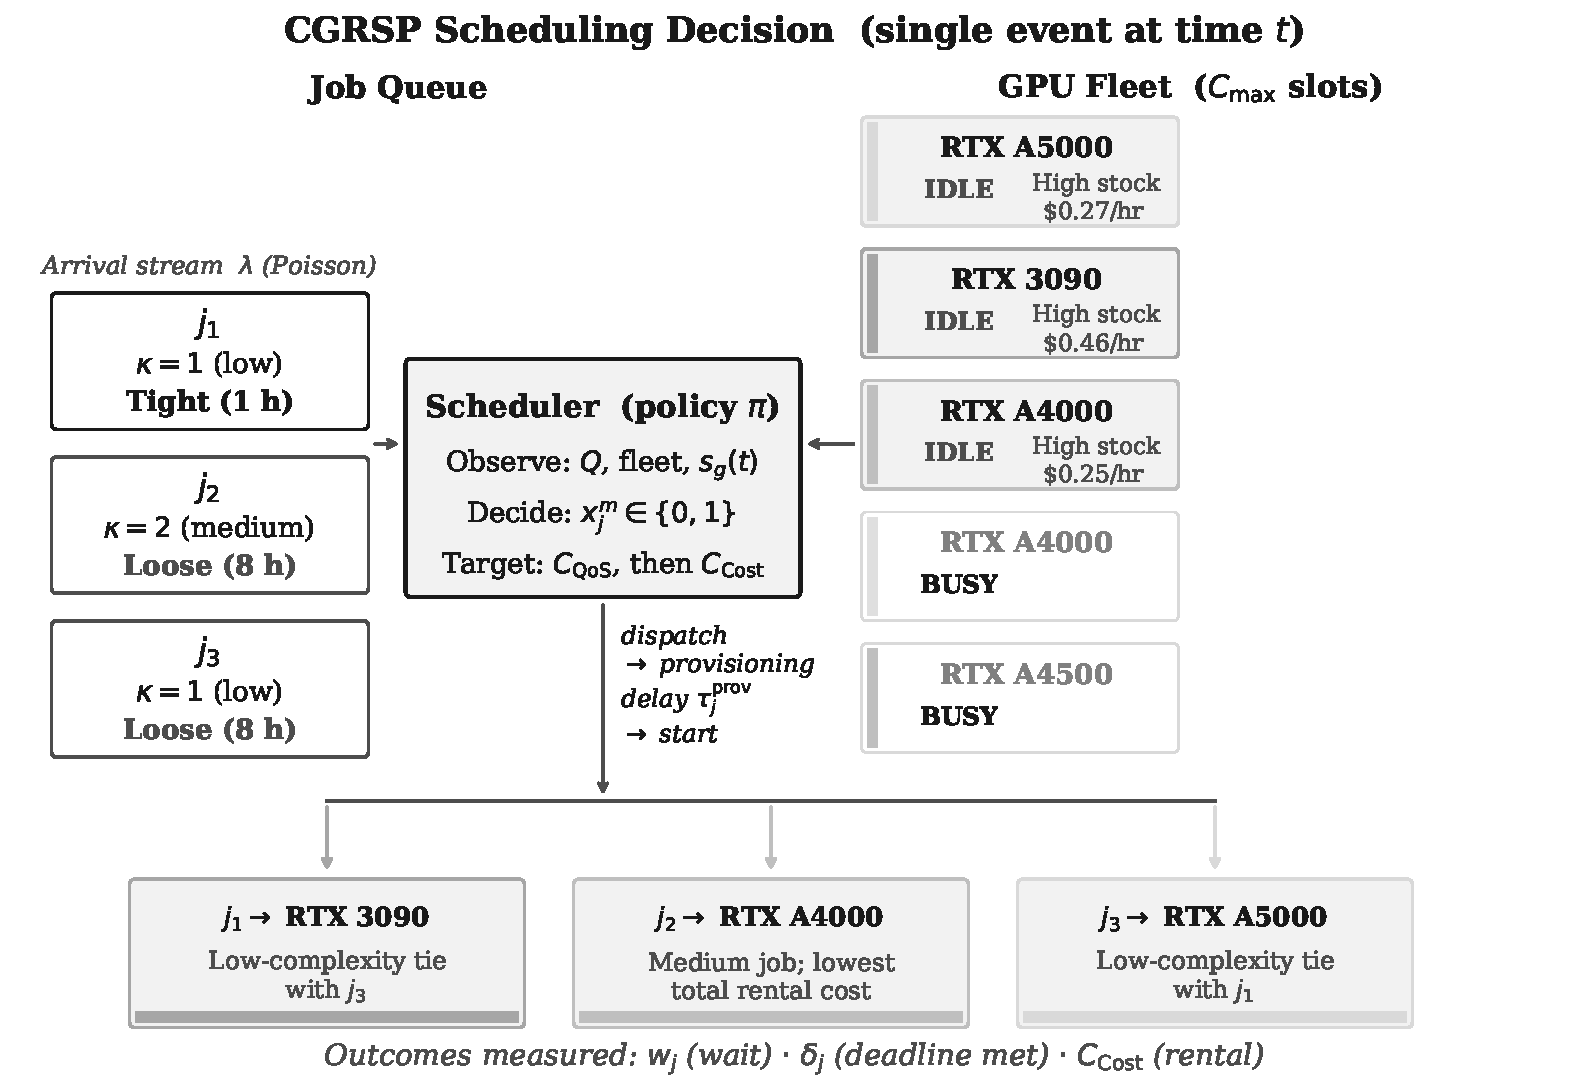
\includegraphics[width=0.98\linewidth,height=0.90\textheight,keepaspectratio]{figures/scheduling_decision.pdf}
\caption[CGRSP scheduling decision at a single event]{CGRSP scheduling decision at a single event.}
\label{fig:scheduling-decision}
\end{figure}
\end{landscape}

\noindent\textit{Figure~\ref{fig:scheduling-decision} notes.} CGRSP scheduling decision at a single event. The scheduler observes the job queue (jobs $j_1$--$j_3$ with complexity $\kappa$ and deadline class) and the GPU fleet ($C_{\max}$ slots with type, stock status, and occupancy). The diagram illustrates the formal lexicographic objective, QoS first (minimise the weighted wait and miss penalty), then cost as a tiebreaker; the implemented policies approximate it rather than solving the joint assignment exactly. The sketch assumes simultaneous dispatch at $t=0$, zero realised provisioning delay, and service times at their class means. Each job then has zero wait and meets its deadline on any of the three idle GPU types, so QoS ties. Minimising total rental cost over the complete assignment puts the medium job $j_2$ on the RTX~A4000 and the two low-complexity jobs on the RTX~3090 and A5000 in either order; the diagram shows one of these cost-tied placements. The tight deadline on $j_1$ does not require the fastest GPU while its one-hour window is non-binding. Busy slots (greyed) are unavailable. Dispatch incurs the provisioning delay $\tau_j^{\text{prov}}$ before a job starts running. The outcomes recorded per job are waiting time $w_j$, deadline adherence $\delta_j$, and rental cost.\par

\begin{table}[htbp]
\centering
\caption{System parameters}
\label{tab:parameters}
\begin{singlespace}
\small
\begin{tabular}{lp{9cm}}
\toprule
\textbf{Symbol} & \textbf{Description} \\
\midrule
$n_g$ & Number of nodes of resource type $g$ \\
$s_g(t)$ & Stock status of resource type $g$ at time $t$ (High / Medium / Low) \\
$p_g$ & Per-second rental price of resource type $g$ \\
$\lambda$ & Mean job arrival rate (jobs per second) \\
$\rho$ & Offered load, $\rho = \lambda\,\overline{W}/C_{\max}$, where $\overline{W}$ is the expected execution time averaged over the complexity mix and, with equal weight, over the $|\calG|$ resource types (not over the $C_{\max}$ slots) \\
$\kappa_j$ & Complexity level of job $j$ \\
$d_j$ & Deadline for job $j$ \\
$t_j^{\text{submit}}$ & Submission time of job $j$ \\
$W(j,g)$ & Realised execution time of job $j$ on resource type $g$; it depends on $j$ only through the complexity level $\kappa_j$, so the class-level form $W(\kappa_j, g)$ is used where convenient \\
$\overline{W}(\kappa,g)$ & Mean (expected) execution time of complexity class $\kappa$ on resource type $g$ \\
$\mu_{\kappa,g}, \sigma_{\kappa,g}$ & Log-space location and dispersion of the execution-time distribution of stratum $(\kappa,g)$; $\mu_{\kappa,g} = \ln \overline{W}(\kappa,g) - \tfrac{1}{2}\sigma_{\kappa,g}^2$ so that $\mathbb{E}[W(j,g)] = \overline{W}(\kappa_j,g)$ (Eq.~\ref{eq:servicetime}) \\
$\beta_g$ & Baseline high-stock probability of resource type $g$ \\
$\phi(t)$ & Time-of-day stock multiplier at time $t$ \\
$\tau^{\text{prov}}_j$ & Provisioning delay incurred when job $j$ acquires an instance (stock-status dependent) \\
$g(m)$ & Resource type of node $m$ \\
$g_j$ & Resource type of the node assigned to job $j$: $g(m)$ for the $m$ with $x_j^m = 1$ \\
$C_{\max}$ & Concurrency limit: number of on-demand slots ($|\calN| = C_{\max}$) \\
$L_s, U_s$ & Lower and upper provisioning-delay bounds for stock status $s$ \\
$p^{H}_g(t), p^{M}_g(t)$ & High-stock probability and Medium-band width (threshold increment) of resource type $g$ at time $t$ \\
$T_{\text{tight}},T_{\text{loose}}$ & Tight and loose deadline-window lengths (rush orders and standard renders); platform values and class proportions in Section~\ref{ssec:platform-and-data} \\
$T_j$ & Deadline window assigned to job $j$, $T_j \in \{T_{\text{tight}}, T_{\text{loose}}\}$ \\
$\alpha_1, \alpha_2$ & QoS penalty weights inside $C_{\text{QoS}}$: penalty per second of waiting ($\alpha_1$) and penalty per missed deadline ($\alpha_2$) \\
$w_{\text{qos}}, w_{\text{cost}}$ & Scalarisation weights balancing QoS and cost, used in the weighted-sum robustness variant (Section~\ref{ssec:objective-weight-sensitivity}) and in the Rolling-Horizon placement surrogate (Chapter~\ref{chap:system}) \\
\bottomrule
\end{tabular}
\end{singlespace}
\end{table}

\begin{table}[htbp]
\centering
\caption{Decision variables and state variables}
\label{tab:variables}
\begin{tabular}{lp{9cm}}
\toprule
\textbf{Symbol} & \textbf{Description} \\
\midrule
$x_j^m \in \{0,1\}$ & Assignment: 1 if job $j$ executes on node $m$ (realised placement over the horizon), 0 otherwise \\
$a_m^t \in \{0,1\}$ & Idle indicator for slot $m$ immediately before dispatch decisions at $t$, after completions at $t$ have released their slots (1 if free, 0 if still held by an earlier job) \\
$t_j^{\text{dispatch}}$ & Dispatch (slot-acquisition) time of job $j$: state variable determined by the scheduling policy \\
$t_j^{\text{start}}$ & Execution start time of job $j$ (Eq.~\ref{eq:starttime}) \\
$t_j^{\text{complete}}$ & Completion time of job $j$ \\
$w_j$ & Waiting time of job $j$ \\
$r_j$ & Response time of job $j$ \\
$\delta_j \in \{0,1\}$ & Deadline adherence indicator: 1 if job $j$ completes on time ($t_j^{\text{complete}} \leq d_j$), 0 otherwise \\
$\tau_j = \max(0, t_j^{\text{complete}} - d_j)$ & Tardiness of job $j$: auxiliary quantity (time past deadline, 0 if on time); defined for completeness, not part of the objective \\
$c_j$ & Execution cost of job $j$ (Eq.~\ref{eq:cost_cost}) \\
$\Delta_{\text{miss}}$ & Deadline miss rate: fraction of jobs that complete after their deadline (Eq.~\ref{eq:missrate}) \\
$C_{\text{QoS}}, C_{\text{Cost}}$ & QoS and operational-cost components of the lexicographic objective (Eqs.~\ref{eq:cqos} and~\ref{eq:ccost}) \\
\bottomrule
\end{tabular}
\end{table}

The system operates as a discrete-event simulator with continuous time representation. At each scheduling event, the scheduler observes the current state and makes assignment decisions. The state space includes both observable information and internal provisioning dynamics.

\textbf{Observable State (Scheduler View):} The scheduler receives a simplified three-state representation for each node:
\begin{itemize}
\item \textbf{Unavailable}: Slot cannot be rented. This state is retained for generality (it arises on a spot market); under the on-demand Secure Cloud model studied here a held slot is never reclaimed, so this state does not occur in the experiments.
\item \textbf{Idle}: Slot is free and can be assigned to jobs
\item \textbf{Running}: Slot is held by an assigned job, either being provisioned or executing
\end{itemize}
Additional observations: current job queue $\calJ_t$ with job characteristics $(\kappa_j, d_j, t_j^{\text{submit}})$, current simulation time $t$, and historical performance metrics.

In addition to per-node availability, the scheduler observes a per-type \textbf{stock status} $s_g(t) \in \{\text{High}, \text{Medium}, \text{Low}\}$ summarising the provisioning reliability of resource type $g$: the likelihood that a fresh instance of type $g$ can be acquired without a long provisioning delay. Stock status is distinct from the idle indicator $a_m^t$: $a_m^t$ records whether a held slot is currently free, whereas $s_g(t)$ reflects market-level scarcity of type $g$. Stock status governs the provisioning delay incurred when a fresh instance of type $g$ is acquired, formalised in Section~\ref{sec:mathematical-model}. In the simulator the status a scheduler observes and the status that fixes the realised delay are two independent draws from the same time-varying model, so the observation behaves as a stale poll rather than a binding quote (Section~\ref{ssec:platform-and-data}). Stock status also biases node selection (Chapter~\ref{chap:system}) away from scarce or unreliable types.

The fleet model enforces at most one job per node at any time: each provisioned instance is exclusively assigned to a single job until completion, and once started a job runs to completion without interruption, since checkpoint-restart mechanisms are expensive or unavailable for rendering workloads. While GPU virtualisation could enable multi-tenancy, the one-job-per-node restriction reflects common rendering workload requirements, where jobs use full GPU capacity for optimal performance.

The model assumes that the on-demand Secure Cloud pool makes every slot rentable at any time: the idle indicator $a_m^t \in \{0,1\}$ records only whether slot $m$ is currently free (1) or held by a job (0), and a held slot is never reclaimed by the provider. Market scarcity is therefore not realised as denial of service but as the provisioning delay $\tau^{\text{prov}}_j$ formalised in Section~\ref{sec:mathematical-model} (Eq.~\ref{eq:provdelay}); the delay ranges and stock-status parameters, stated as modelling assumptions informed qualitatively by the RunPod snapshot record, are given in Chapter~\ref{chap:experiments}.

\textbf{Human Decision Elements:} The formulation reflects human operational decisions through several design parameters:
\begin{itemize}
\item \textbf{Deadline policy}: Per-job deadline window from submission time ($d_j = t_j^{\text{submit}} + T_j$, where $T_j \in \{T_{\text{tight}}, T_{\text{loose}}\}$; values and class proportions are given in Section~\ref{ssec:platform-and-data})
\item \textbf{Fleet configuration} ($n_g$ for each $g \in \calG$): Capacity planning decision
\item \textbf{Deadline-penalty weights} ($\alpha_1, \alpha_2$): the business valuation of a missed deadline against accumulated waiting inside $C_{\text{QoS}}$; the scalar weights $w_{\text{qos}}, w_{\text{cost}}$ exist only in the robustness variant and the RH surrogate
\end{itemize}

\section{Mathematical Model}
\label{sec:mathematical-model}

The scheduling objective is bi-objective, with quality of service treated as the \emph{primary} criterion and operational cost as a \emph{secondary}, tiebreaking criterion. QoS is optimised first; operational cost is optimised only among assignments that are equivalent on QoS. This lexicographic priority is a modelling preference for service quality over rental spend, not a measured contractual penalty: the chosen $\alpha_2/\alpha_1=10$ equates one missed deadline with only ten seconds of waiting within the QoS component, as explained below. Formally, the model defines the following lexicographic objective; the online schedulers in Chapter~\ref{chap:system} use heuristics or surrogate scores rather than solving this joint optimisation exactly:
\begin{align}
\operatorname*{lex\,min}\; \bigl( C_{\text{QoS}},\; C_{\text{Cost}} \bigr) & \label{eq:objective}\\
C_{\text{QoS}} &= \sum_{j \in \calJ} \bigl[\, \alpha_1\, w_j + \alpha_2\, (1 - \delta_j) \,\bigr] \label{eq:cqos}\\
C_{\text{Cost}} &= \sum_{j \in \calJ} c_j \label{eq:ccost}
\end{align}
where lexicographic minimisation prefers any policy with lower $C_{\text{QoS}}$ and breaks QoS ties on lower $C_{\text{Cost}}$. The QoS cost (Eq.~\ref{eq:cqos}) combines a waiting-time penalty and a deadline-violation penalty: $w_j$ is the waiting time in seconds (Eq.~\ref{eq:wait}), $\alpha_1$ is the penalty per second of wait, and $\alpha_2$ is a penalty per missed deadline applied through the binary miss indicator $(1 - \delta_j)$. The concrete values of $\alpha_1$ and $\alpha_2$ used in experiments are given in Section~\ref{ssec:platform-and-data}; their ratio $\alpha_2/\alpha_1$ is swept in Section~\ref{ssec:objective-weight-sensitivity} to verify robustness. At the calibrated ratio $\alpha_2/\alpha_1 = 10$, one missed deadline is worth ten seconds of waiting, so the $C_{\text{QoS}}$ ordering of policies is essentially their mean-wait ordering; the headline ranking and the recommendations therefore use the miss rate $\Delta_{\text{miss}}$ directly rather than the scalar $C_{\text{QoS}}$. The cost criterion $C_{\text{Cost}}$ is the total rental spend across all provisioned instances, summing the per-job execution cost $c_j$, which is defined formally in Eq.~\ref{eq:cost_cost} below, once the assignment variable $x_j^m$ has been introduced through the constraints.

Subject to:
\begin{align}
\sum_{m \in \calN} x_j^m &= 1, & \forall j \in \calJ \label{eq:single_assign}\\
\sum_{j \in \calJ} x_j^m \, \mathbf{1}\!\left[t_j^{\text{dispatch}} \leq t < t_j^{\text{complete}}\right] &\leq 1, & \forall m \in \calN,\; \forall t \label{eq:single_job_node}\\
x_j^m &\leq a_m^{t_j^{\text{dispatch}}}, & \forall j \in \calJ,\; m \in \calN \label{eq:avail}
\end{align}
\begin{align}
p^{H}_g(t) &= \min\!\left(0.95,\, \beta_g\, \phi(t)\right), & p^{M}_g(t) &= \min\!\left(0.90,\, 1.5\,\beta_g\, \phi(t)\right), & \forall g \in \calG,\ \forall t \label{eq:stockprob}
\end{align}
\begin{equation}
\begin{gathered}
s_g(t) =
\begin{cases}
\text{High} & \text{if } u_{g,k} < p^{H}_g(t),\\
\text{Medium} & \text{if } p^{H}_g(t) \le u_{g,k} < p^{H}_g(t) + p^{M}_g(t),\\
\text{Low} & \text{otherwise},
\end{cases}\\[0.5ex]
\forall g \in \calG,\ \forall t,\quad u_{g,k} \overset{\text{i.i.d.}}{\sim} \text{Uniform}(0,1)\ \text{for the $k$-th draw made at time $t$}
\end{gathered}
\label{eq:stock}
\end{equation}
\begingroup
\allowdisplaybreaks
\begin{align}
W(j,g) &\sim \text{LogNormal}\!\left(\mu_{\kappa_j,g},\, \sigma_{\kappa_j,g}^2\right), & \forall j \in \calJ,\; g \in \calG \label{eq:servicetime}\\
\tau^{\text{prov}}_j &\sim \text{Uniform}\!\left(L_{\tilde s_{g_j}(t_j^{\text{dispatch}})},\; U_{\tilde s_{g_j}(t_j^{\text{dispatch}})}\right), & \forall j \in \calJ \label{eq:provdelay}\\
t_j^{\text{dispatch}} &\geq t_j^{\text{submit}}, & \forall j \in \calJ \label{eq:release}\\
t_j^{\text{start}} &= t_j^{\text{dispatch}} + \tau^{\text{prov}}_j, & \forall j \in \calJ \label{eq:starttime}\\
t_j^{\text{complete}} &= t_j^{\text{start}} + \sum_{m \in \calN} x_j^m W(j,g(m)), & \forall j \in \calJ \label{eq:completion}\\
d_j &= t_j^{\text{submit}} + T_j, & \forall j \in \calJ \label{eq:deadline_window}\\
w_j &= t_j^{\text{start}} - t_j^{\text{submit}}, & \forall j \in \calJ \label{eq:wait}\\
r_j &= t_j^{\text{complete}} - t_j^{\text{submit}}, & \forall j \in \calJ \label{eq:resp}\\
\tau_j &= \max(0,\, t_j^{\text{complete}} - d_j), & \forall j \in \calJ \label{eq:tardiness}\\
\delta_j &= \mathbf{1}[t_j^{\text{complete}} \leq d_j], & \forall j \in \calJ \label{eq:adherence}\\
\Delta_{\text{miss}} &= \frac{1}{|\calJ|}\sum_{j \in \calJ} (1 - \delta_j) \label{eq:missrate}\\
c_j &= \sum_{m \in \calN} x_j^m \, W(j, g(m))\, p_{g(m)}, & \forall j \in \calJ \label{eq:cost_cost}\\
x_j^m,\; a_m^t,\; \delta_j &\in \{0,1\},\ \ w_j,\, r_j,\, \tau_j,\, c_j \geq 0, & \forall j \in \calJ,\; m \in \calN,\; t \label{eq:domains}
\end{align}
\endgroup

Constraints~(\ref{eq:single_assign})--(\ref{eq:avail}) ensure feasible assignments respecting the concurrency limit and slot occupancy. The assignment variable $x_j^m$ records the realised placement over the whole horizon, so Constraint~(\ref{eq:single_job_node}) is stated per time instant using the indicator function $\mathbf{1}[\cdot]$, a standard piece of notation that evaluates to $1$ when the bracketed condition is true and $0$ otherwise. Concretely, $\mathbf{1}\!\left[t_j^{\text{dispatch}} \leq t < t_j^{\text{complete}}\right]$ equals $1$ exactly while node $m$ is held by job $j$, i.e.\ from its dispatch (the slot acquisition, so the provisioning window is included) up to (but not including) its completion time, and $0$ at every other instant. Multiplying by $x_j^m$ and summing over $j \in \calJ$ therefore counts how many jobs simultaneously hold node $m$ at instant $t$; bounding that count by $1$ states, in plain terms, that node $m$ can be held by at most one job at any given time, whether that job is still being provisioned or already executing. The half-open occupancy interval $[t_j^{\text{dispatch}}, t_j^{\text{complete}})$ inside the indicator lets a slot that completes a job at $t$ accept its successor at the same instant without double counting. Constraint~(\ref{eq:avail}) requires the chosen slot to be idle in the pre-decision state at the job's dispatch instant ($a_m^{t_j^{\text{dispatch}}} = 1$). Constraint~(\ref{eq:single_assign}) is a covering equality over the complete service horizon: every submitted job must eventually execute exactly once, and rejection is not allowed. This does not force immediate dispatch at an online event. An online policy uses only its observable state and history; the realised assignment variables describe its eventual schedule, not advance knowledge of the sampled service times. A job can remain in $\calJ_t$ until its chosen dispatch time; the realised horizon-wide placement $x_j^m$ is distinct from an event's decision to defer it. Constraint~(\ref{eq:release}) prevents dispatch before submission, while Equation~(\ref{eq:completion}) binds completion to execution start plus the realised service time on the assigned node. Since that service time is strictly positive, a job cannot occupy an empty interval or complete before starting. The concurrency limit $C_{\max}$ is encoded directly in $|\calN|$: the node set $\calN$ contains exactly $C_{\max}$ virtual on-demand slots, so at most $C_{\max}$ jobs can run simultaneously at any time $t$. Slots are costless when idle; rental charges apply only while a job is executing on one.

Equation~(\ref{eq:servicetime}) makes the realised execution time a log-normal random variable whose expectation is the stratum mean $\overline{W}(\kappa_j,g)$: the log-space location $\mu_{\kappa,g} = \ln \overline{W}(\kappa,g) - \tfrac{1}{2}\sigma_{\kappa,g}^2$ is fixed by that expectation, and the log-space dispersion $\sigma_{\kappa,g}$ is fitted per stratum in Chapter~\ref{chap:experiments}, so a job's expected duration is known at dispatch while its realised duration is not. Equations~(\ref{eq:stockprob}), (\ref{eq:stock}), (\ref{eq:provdelay}) and~(\ref{eq:starttime}) formalise the stochastic provisioning process that Section~\ref{sec:problem-description} introduced informally, made explicit here because the provisioning delay $\tau^{\text{prov}}_j$ it produces is a first-class component of the waiting time $w_j$, not an implementation detail. Each resource type $g$ carries a stock status $s_g(t)$ drawn by comparing one fresh uniform variate $u_{g,k} \sim \text{Uniform}(0,1)$, independent across types and across the draws $k$ made at successive dispatch events, against cumulative thresholds set by a baseline high-stock probability $\beta_g$ and a time-of-day multiplier $\phi(t)$; Equation~(\ref{eq:stockprob}) defines the two thresholds, capping the High-stock probability at $0.95$ and the Medium-band width at $0.90$, and Equation~(\ref{eq:stock}) draws the status from them. Because $p^{M}_g$ is the width of the Medium band and not the probability of Medium, the two thresholds are not clipped to a total of $1$: where $p^{H}_g + p^{M}_g \ge 1$ (for example the RTX~3090 in an off-peak hour, $0.65 + 0.90$) the draw never returns Low and the realised probability of Medium is $1 - p^{H}_g$; this is a deliberate property of the calibrated model and is disclosed with the availability assumptions in Section~\ref{ssec:platform-and-data}. When job $j$ is dispatched at time $t_j^{\text{dispatch}}$ to a slot of its assigned type $g_j$, it incurs the provisioning delay $\tau^{\text{prov}}_j$ drawn against a stock status $\tilde s_{g_j}(t_j^{\text{dispatch}})$ of that type at the dispatch instant, sampled from the same process as $s_g(t)$ but by an independent draw, so it need not equal the status the scheduler last observed (Eq.~\ref{eq:provdelay}), whose range depends on the stock status (per-status ranges in Section~\ref{ssec:platform-and-data}; the Low-state delays are orders of magnitude longer than High-state ones); the realised start time then follows from the dispatch time and this delay (Eq.~\ref{eq:starttime}), so $\tau^{\text{prov}}_j$ forms a component of the waiting time $w_j$ (Eq.~\ref{eq:wait}). The $\beta_g$ values, the $\phi(t)$ bands, and the resulting frequency of each stock state are parameter values given in Chapter~\ref{chap:experiments}, where they are stated as modelling assumptions rather than empirical frequencies.

Equation~(\ref{eq:deadline_window}) fixes each job's absolute deadline from its per-job deadline window $T_j$. Unlike hard-deadline models, the CGRSP formulation treats deadlines as soft: violations are penalised in the objective rather than structurally prohibited. This reflects operational reality under the $C_{\max}$ concurrency ceiling: when the offered load $\rho = \lambda\,\overline{W}/C_{\max}$ exceeds one the queue tends to grow for as long as the arrival burst lasts, and with online arrivals, stochastic provisioning delays and stochastic service times some misses are then a routine outcome of real operation even where capacity alone forces none (on the hectic day the window-capacity bound of Section~\ref{ssec:capacity-lower-bound} certifies zero unavoidable misses). A penalty formulation that grades misses, rather than a hard constraint that would declare such realisations infeasible, is therefore the appropriate model.

Equations~(\ref{eq:wait})--(\ref{eq:adherence}) define the QoS metrics tracked for each job. Equation~(\ref{eq:missrate}) aggregates the per-job indicators into the deadline miss rate $\Delta_{\text{miss}}$, the fraction of jobs that complete after their deadline; it is the primary QoS statistic reported in Chapter~\ref{chap:experiments}. The response time $r_j$ (Eq.~\ref{eq:resp}) is the job's total sojourn from submission to completion, the sum of its waiting time $w_j$ and its realised execution time; it does not enter the objective and is tracked as a diagnostic, reported in Chapter~\ref{chap:experiments} through those two components rather than as a separate column. Figure~\ref{fig:job-lifecycle} illustrates how each interval maps onto a job's timeline for both the on-time and the missed-deadline cases. Deadline violations are penalised in the objective via the binary miss indicator $(1 - \delta_j)$ rather than via continuous tardiness $\tau_j$; tardiness (Eq.~\ref{eq:tardiness}) is defined for completeness but is not used in the objective. The miss-indicator form is the appropriate QoS penalty in a rendering-studio context because a missed client deadline is a discrete, qualitatively costly event (contract penalties, pipeline delays) rather than a quantity that scales with how late the job is; once a job will miss, its exact lateness is of secondary operational concern, so the objective penalises whether a deadline is met, not by how much. A corollary is that the scheduler should not sacrifice jobs that can still be saved in order to reduce the lateness of jobs that are already doomed. Mean tardiness is nonetheless reported as a diagnostic metric in Chapter~\ref{chap:experiments}, because the severity of missed deadlines matters operationally even when the count of misses is the primary objective. A robustness study (Chapter~\ref{chap:experiments}, Section~\ref{ssec:objective-weight-sensitivity}) re-scores a six-policy subset (FIFO, SPT, EDF, SPT+Rescue, RH and CADR) against a tardiness-based objective, and the per-metric leaders within that subset are unchanged: RH retains the lowest miss-rate point estimate and CADR attains the lowest mean tardiness on that ten-seed re-scoring set (at the 30-seed Phase~3 scale EDF's tardiness is marginally lower, Table~\ref{tab:statistical}). The subset boundary matters and is stated explicitly here, because that study omits the Adaptive EDF-SPT hybrid, which records a lower mean tardiness than CADR in the full ten-scheduler comparison (Section~\ref{sec:phase-3-statistical-validation}) while matching neither proposed scheduler on miss rate; CADR is therefore the lowest-tardiness policy of the re-scored six on that set, not of the fleet of policies evaluated in this thesis. What the tardiness objective does shift is the single scalarised winner, which moves towards low-tardiness policies; the decomposed conclusions of this thesis are therefore robust to the deadline-penalty form, while any single collapsed score is not.

\begin{landscape}
\begin{figure}[H]
\centering
\captionsetup{font=small,skip=6pt}
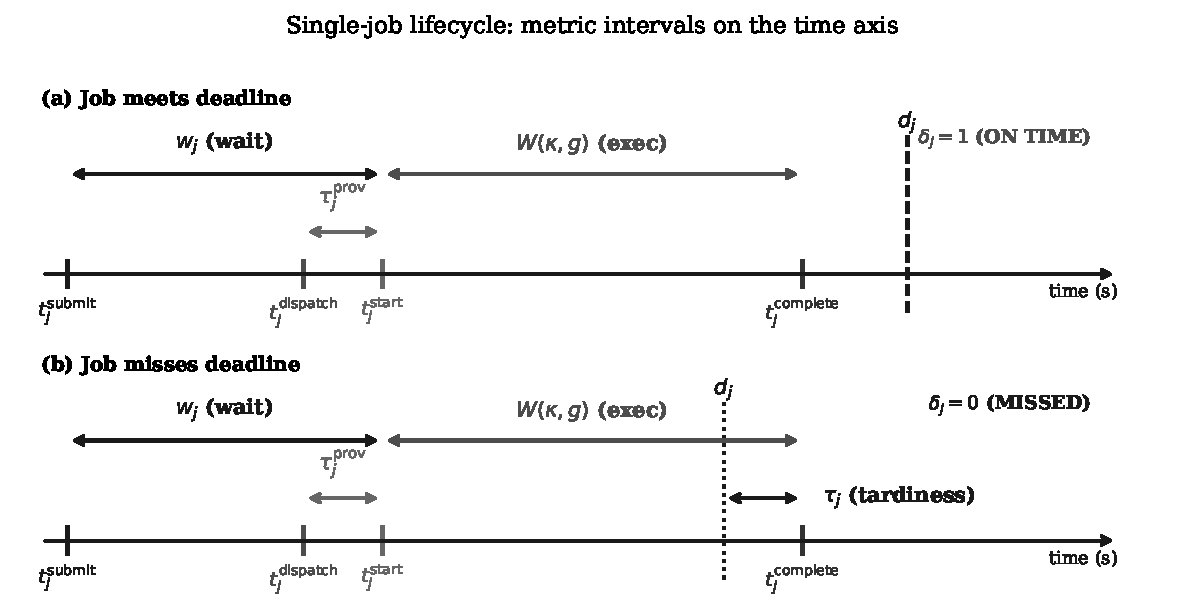
\includegraphics[width=0.98\linewidth,height=0.72\textheight,keepaspectratio]{figures/job_lifecycle.pdf}
\caption[Single-job lifecycle and metric intervals]{Single-job lifecycle: metric intervals mapped onto the time axis. Panel~(a) shows a job that meets its deadline ($\delta_j=1$): the waiting time $w_j$ spans submission to execution start and includes the provisioning delay $\tau^{\text{prov}}_j$ incurred between dispatch ($t_j^{\rm dispatch}$, slot acquisition) and execution start ($t_j^{\rm start}$); the execution time $W(\kappa,g)$ then runs to completion before the deadline $d_j$. Panel~(b) shows a missed deadline ($\delta_j=0$): completion falls after $d_j$, and tardiness $\tau_j = t_j^{\rm complete} - d_j > 0$.}
\label{fig:job-lifecycle}
\end{figure}
\end{landscape}

Equation~(\ref{eq:cost_cost}) defines the per-job execution cost $c_j$ that Eq.~\ref{eq:ccost} sums over $\calJ$ into the operational cost component $C_{\text{Cost}}$: the per-second rental fees for the provisioned GPU instances across all nodes, where $W(j, g(m))$ is the realised execution time of job $j$ on the assigned node's type (the stochastic execution-time model is calibrated in Chapter~\ref{chap:experiments}). Note the asymmetry in how the provisioning delay is accounted: $\tau^{\text{prov}}_j$ counts fully towards the waiting time $w_j$ (Eqs.~\ref{eq:starttime} and~\ref{eq:wait}) and hence towards the QoS penalty, but it is \emph{not} billed, since rental charges accrue only over the execution interval $[t_j^{\text{start}}, t_j^{\text{complete}}]$; a scarce GPU type therefore hurts the scheduler through QoS, not through cost. Finally, Constraint~(\ref{eq:domains}) states the natural domains of the decision and state variables.

Because the value of a missed deadline relative to accumulated waiting (the ratio $\alpha_2/\alpha_1$) is a business policy rather than a physical constant, no single value is canonical; the deadline-penalty ratio is swept in the objective-weight sensitivity analysis (Section~\ref{ssec:objective-weight-sensitivity}), which additionally evaluates a fully symmetric weighted-sum scalarisation $\min \bigl[\, w_{\text{qos}}\, C_{\text{QoS}} + w_{\text{cost}}\, C_{\text{Cost}} \,\bigr]$ with $w_{\text{qos}} = w_{\text{cost}} = 0.5$ as a robustness variant. Although RH wins the tested binary-miss grid, a symmetric scalar can in general let a small cost difference reorder policies separated on QoS; the lexicographic objective avoids this by construction, which is why all headline comparisons are reported on the decomposed metrics (mean wait, miss rate, and cost) rather than on a scalar value.

\section{Modelling Simplifications and Assumptions}
\label{sec:modelling-simplifications-and-assumptions}

The formulation rests on five modelling simplifications, collected here so that the assumptions behind every later result are stated once in one place rather than reconstructed from the simulator design (Chapter~\ref{chap:system}) or from the experimental chapters that follow. Each remark states the simplification, why it is defensible for the rendering workload studied, and what relaxing it would require.

\begin{enumerate}
\item \textbf{Remark 1, stochastic execution times.} The realised execution time $W(j,g)$ is a random variable, not a constant fixed by the pair (complexity level, resource type). It is drawn from the per-stratum log-normal service-time model of Equation~(\ref{eq:servicetime}), whose expectation is the stratum mean $\overline{W}(\kappa_j, g)$ and whose dispersion parameters are fitted in Chapter~\ref{chap:experiments}. What the pair does fix is that expectation, so a job's realised duration is uncertain while its expected duration is known: schedulers plan with $\overline{W}(\kappa_j, g)$ and observe the realised value only on completion, mirroring a dispatcher that can classify a scene's complexity before rendering but cannot know its exact walltime. Relaxing this towards heavier-tailed or correlated service times would change the variance of the QoS metrics rather than the structure of the model.

\item \textbf{Remark 2, one job per node.} Constraint~(\ref{eq:single_job_node}) admits at most one job holding a node at any instant, from dispatch to completion, so a provisioned instance is held exclusively for the duration of its job. This reflects rendering practice, where a job consumes the full GPU for best performance, and it is what makes the concurrency ceiling $C_{\max}$ a meaningful capacity limit. GPU virtualisation would permit multi-tenancy and would require a per-node resource-share variable in place of the binary $x_j^m$.

\item \textbf{Remark 3, no preemption.} Once execution begins, a job runs to completion without interruption, migration, or restart, because checkpoint-restart is expensive or unavailable for rendering pipelines. A consequence used throughout the scheduler designs is that a placement decision is irrevocable for the length of the job, so anticipation must happen before dispatch rather than through later correction.

\item \textbf{Remark 4, Poisson arrivals.} Jobs arrive as a Poisson process with mean rate $\lambda$, that is, with independent, memoryless, exponentially distributed inter-arrival times, the canonical model for independent submissions from separate clients and scenes. The day-type values of $\lambda$ used in the experiments are set in Chapter~\ref{chap:experiments}. Bursty or self-similar arrival processes would raise queueing delay at the same mean rate and are not modelled here.

\item \textbf{Remark 5, binary availability.} The idle indicator satisfies $a_m^t \in \{0,1\}$, so the scheduler observes a definite idle or running status for every slot rather than a partial or probabilistic one. Market scarcity is not modelled as denial of service under the on-demand Secure Cloud pool studied here, since a held slot is never reclaimed; it enters instead through the stochastic provisioning delay $\tau^{\text{prov}}_j$ of Eq.~(\ref{eq:provdelay}), which is itself driven by the per-type stock status $s_g(t)$ of Eq.~(\ref{eq:stock}). A spot-market variant would restore the Unavailable state of Section~\ref{sec:problem-description} and make availability itself stochastic.
\end{enumerate}

\section{Numerical Example}
\label{sec:numerical-example}

A minimal three-job, two-GPU instance makes the interplay of constraints visible. Two resource types are in the fleet: an RTX~3090 ($g_1$) and an RTX~A4000 ($g_2$). The concurrency cap is $C_{\max}$ (five slots in the experimental platform, Section~\ref{ssec:platform-and-data}); only three are used here, leaving two idle. Slots $m_2$ and $m_3$ are RTX~A4000 slots; $m_1$, $m_4$ and $m_5$ are RTX~3090 slots. Three jobs $\calJ = \{j_1, j_2, j_3\}$ arrive simultaneously at $t = 0$; nodes begin available ($a_m^0 = 1$ for all $m \in \calN$), and every resource type starts at High stock ($s_g(0) = \text{High}$).

\textbf{Job Characteristics:}
\begin{center}
\begin{tabular}{llll}
\toprule
\textbf{Job}&\textbf{Complexity}&\textbf{Submit Time}&\textbf{Deadline}\\
\midrule
$j_1$&$\kappa = 1$ (Low)&$t=0$&$t=3600$ (tight)\\
$j_2$&$\kappa = 2$ (Medium)&$t=0$&$t=28800$ (loose)\\
$j_3$&$\kappa = 1$ (Low)&$t=0$&$t=28800$ (loose)\\
\bottomrule
\end{tabular}
\end{center}

\textbf{Expected Execution Times} $\overline{W}(\kappa, g)$ (seconds; realised times are taken at their expected values in this example; see Table~\ref{tab:gpu_specs} for full GPU specifications):
\begin{center}
\begin{tabular}{lcc}
\toprule
\textbf{Complexity}&\textbf{RTX 3090 ($g_1$)}&\textbf{RTX A4000 ($g_2$)}\\
\midrule
Low ($\kappa=1$)&59.5&63.3\\
Medium ($\kappa=2$)&69.6&72.1\\
High ($\kappa=3$)&91.2&98.6\\
\bottomrule
\end{tabular}
\end{center}

Figure~\ref{fig:numerical-example} illustrates the assignment and timeline.

\begin{landscape}
\begin{figure}[H]
\centering
\captionsetup{font=small,skip=6pt}
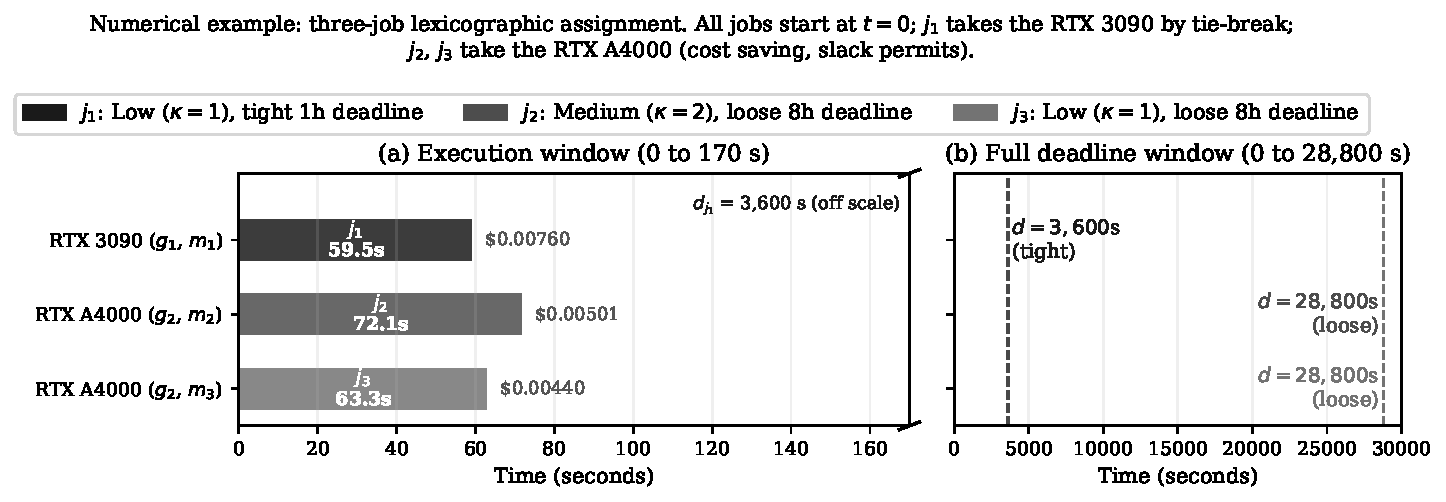
\includegraphics[width=0.98\linewidth,height=0.72\textheight,keepaspectratio]{figures/numerical_example.pdf}
\caption[Numerical example: three-job schedule on two GPUs]{Visual aid for the three-job numerical example. (a)~Execution window: all three jobs start immediately (High stock, negligible provisioning delay). $j_1$ (dark grey) runs on the RTX~3090 for 59.5\,s; $j_2$ (mid grey) and $j_3$ (light grey) run concurrently on separate RTX~A4000 slots for 72.1\,s and 63.3\,s respectively. Dollar annotations show per-job cost. The tight deadline $d_{j_1}=3{,}600$\,s is indicated by a dashed black line. (b)~Full deadline window: $j_2$ and $j_3$ each have an 8-hour loose deadline (28{,}800\,s), vastly exceeding their execution times and confirming that cost is the only discriminating criterion for those two jobs.}
\label{fig:numerical-example}
\end{figure}
\end{landscape}

\textbf{Assignment under the lexicographic objective.}
Every job here starts at $t=0$ and finishes within about a minute, so all three meet their deadlines with zero waiting on either GPU type. This includes $j_1$, whose one-hour window does not bind at this load. The three jobs are therefore QoS-equivalent across the fleet, since $w_j$ (Eq.~\ref{eq:wait}) excludes execution time, and the secondary cost criterion decides every placement. The A4000 saving is largest for the medium job, so $j_2$ takes one of the two RTX~A4000 slots. The other goes to a low-complexity job, and the remaining low-complexity job takes an RTX~3090 slot. Because $j_1$ and $j_3$ cost the same there, the objective leaves a tie, broken here in favour of the tight job ($x_{j_1}^{m_1} = x_{j_2}^{m_2} = x_{j_3}^{m_3} = 1$). Note that $j_2$'s medium complexity creates no tension here, whichever GPU is faster: both A4000 means used above rest on the relative-performance estimate, because the medium-complexity A4000 cell has only $n=2$ observed jobs (below the reliability threshold; their raw mean is 73.1\,s, against 69.6\,s for the RTX~3090, while the estimate is 72.1\,s) and there is no observed low-complexity A4000 job at all. Even if the RTX~3090 is faster in a stratum, eight hours of slack would strip that speed advantage of any QoS value and the cost tiebreaker would still prevail. The two remaining slots are left idle ($x_j^{m_4} = x_j^{m_5} = 0$ for every $j$).

\textbf{Outcome.}
All three jobs start immediately: every type begins at High stock, where the provisioning delay (Eq.~\ref{eq:provdelay}) is at most 10\,s (Section~\ref{ssec:platform-and-data}) and is taken as zero here, so every waiting-time penalty is zero ($w_{j_1} = w_{j_2} = w_{j_3} = 0$~s) and all deadlines are met (the QoS objective is at its optimum). Rental cost then works out to
$59.5 \times 0.000128 + 72.1 \times 0.0000694 + 63.3 \times 0.0000694 = \$0.017$,
where the per-second rates are derived from the RTX~3090 price of \$0.46/hr and the RTX~A4000 price of \$0.25/hr (Table~\ref{tab:gpu_specs}). Fleet utilisation is $3/5 = 60\%$. The key observation is that at this load every cost saving comes at no QoS penalty. Only once waiting or provisioning delay began to threaten $j_1$'s one-hour window would its tight deadline override cost. This ordering, QoS first and cost only among QoS-equivalent options, drives the scheduler designs described in Chapter~\ref{chap:system}.

\chapter{System Design and Scheduling Algorithms}
\label{chap:system}

\section{System Architecture Overview}
\label{sec:system-architecture-overview}

The CGRSP evaluation system comprises five tightly coupled components (Figure~\ref{fig:architecture}). The components communicate through a single shared event queue: the Job Generator places arrival events, the DES Core dispatches them and invokes the Scheduler, the Scheduler queries the Fleet Manager for idle nodes, and the Metrics Collector receives completion notifications.



\begin{enumerate}
  \item \textbf{Job Generator}: produces a Poisson job stream with configurable arrival rate, complexity distribution, and deadline distribution.
  \item \textbf{Discrete-Event Simulator Core}: maintains a min-heap priority event queue and advances simulation time from event to event.
  \item \textbf{Fleet Manager}: tracks active instance slots up to $C_{\max}$, models per-type stock availability, and reports available slots to the scheduler. An ``idle'' slot has no GPU instance provisioned and incurs no cost; it represents unused concurrency capacity.
  \item \textbf{Scheduler}: implements the scheduling policy; receives the current queue and fleet state at each scheduling decision point and returns a list of (job, node) assignments.
  \item \textbf{Metrics Collector}: receives completion notifications and records per-job outcomes (waiting time, deadline adherence, cost) for reporting.
\end{enumerate}

The simulator core is adapted from SPARS~\cite{amrizal2026spars}, a lightweight discrete-event simulator for HPC job scheduling; its node power-state manager and energy accounting are replaced by the CGRSP fleet, stock-status provisioning model and QoS/cost metrics described in this chapter. The adapted simulator is implemented in Python using only the standard library and NumPy, so the build has no external simulation-framework dependency, which keeps full control over event semantics and metric computation.


\begin{landscape}
\begin{figure}[H]
\centering
\captionsetup{font=small,skip=6pt}
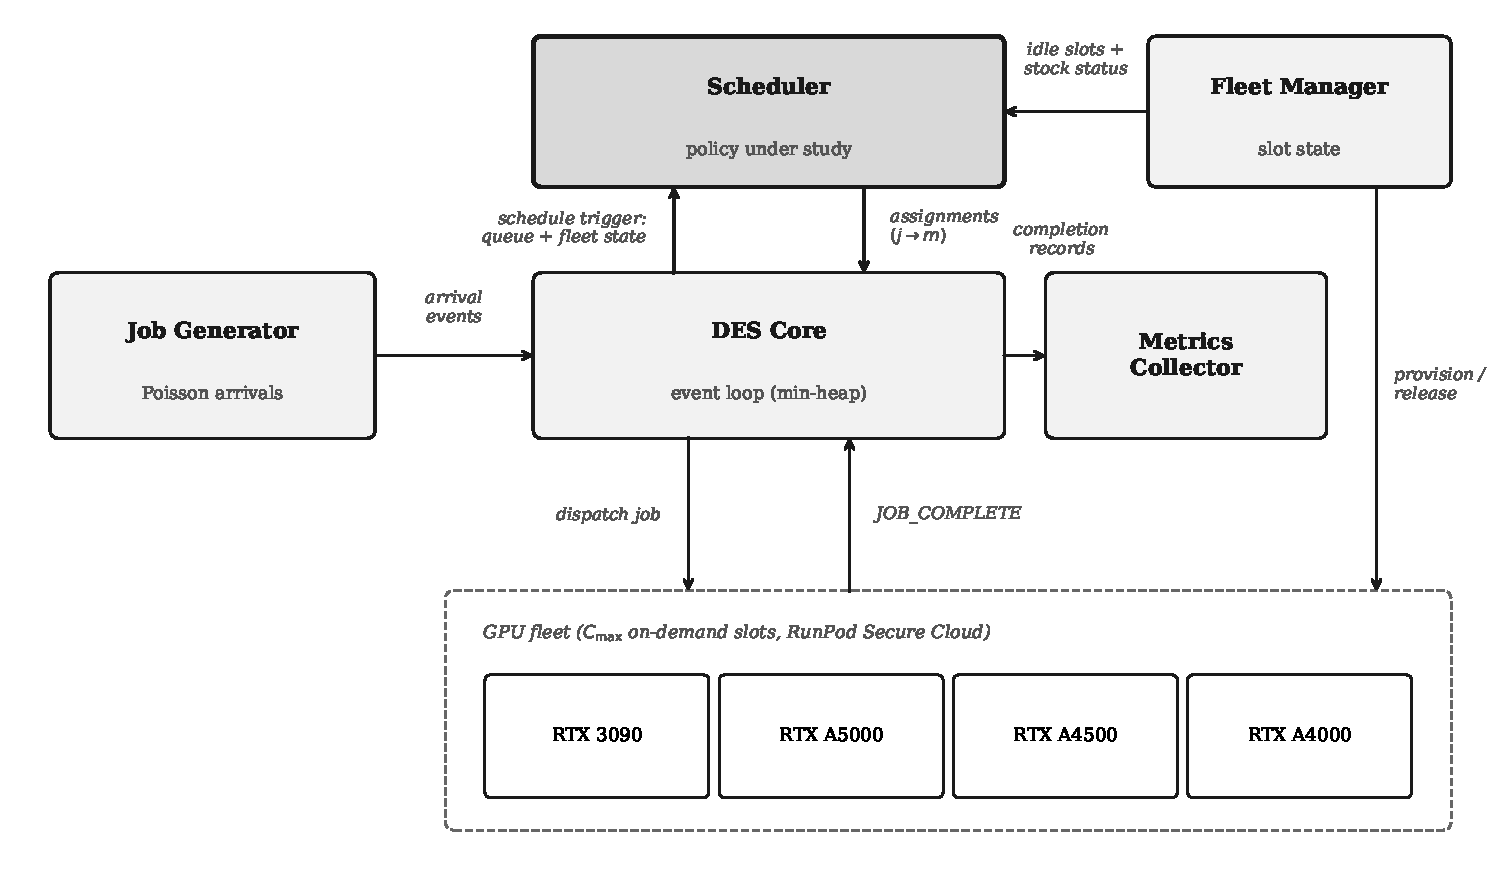
\includegraphics[width=0.98\linewidth,height=0.82\textheight,keepaspectratio]{figures/system_architecture.pdf}
\caption[CGRSP system architecture]{CGRSP system architecture: five components interact through a shared discrete-event queue. The Job Generator produces a Poisson job stream; the DES Core advances simulation time and invokes the Scheduler at each event; the Scheduler queries the Fleet Manager for idle slots and returns assignments; the Metrics Collector records per-job outcomes. The GPU fleet (dashed box) comprises four heterogeneous GPU types operating under stochastic stock-status provisioning-delay dynamics.}
\label{fig:architecture}
\end{figure}
\end{landscape}

\section{Discrete-Event Simulator Core}
\label{sec:discrete-event-simulator-core}

The simulator maintains a min-heap event queue ordered by event timestamp. Three event types drive the scheduling dynamics (the implementation also defines node transition, inert under the on-demand fleet, and simulation end, which closes every run; same-instant events are ordered by a priority field after the timestamp). The names below are descriptive aliases for the implementation's \texttt{JOB\_ARRIVAL}, \texttt{JOB\_COMPLETION} and \texttt{SCHEDULER\_DECISION}:

\begin{itemize}
  \item \texttt{JOB\_ARRIVAL}$(j, t)$: Job $j$ arrives at time $t$. The job is added to the waiting queue, and scheduling decision events are generated immediately (two at the same instant in the implementation, the second redundant for deterministic policies).
  \item \texttt{JOB\_COMPLETE}$(j, m, t)$: Job $j$ completes on node $m$ at time $t$. Node $m$ is freed, metrics are recorded, and a \texttt{SCHEDULE\_TRIGGER} event is generated.
  \item \texttt{SCHEDULE\_TRIGGER}$(t)$: The scheduler is invoked at time $t$. If any idle nodes and waiting jobs exist, the scheduler returns an assignment; the simulation then generates the corresponding \texttt{JOB\_COMPLETE} event at $t + \tau^{\text{prov}}_j + W(\kappa_j, g(m))$ (Eq.~\ref{eq:starttime}).
\end{itemize}

A job dispatched to a slot of type $g$ does not start instantly: it incurs a provisioning delay drawn from the stock-status-dependent range of Eq.~\ref{eq:provdelay} before entering the \textbf{running} state. No node-failure or node-restoration events occur, because the on-demand Secure Cloud pool never reclaims a held slot (Section~\ref{sec:problem-description}).

\section{GPU Fleet Model}
\label{sec:gpu-fleet-model}

The fleet manager instantiates nodes according to the GPU type configuration. Each node is parameterised by:

\begin{itemize}
  \item \textbf{GPU type} $g \in \calG$: determines $p_g$ and the execution time $W(\kappa, g)$.
  \item \textbf{Stock status}: High / Medium / Low, updated stochastically; it sets the provisioning delay (Eq.~\ref{eq:provdelay}; the status a scheduler observes is an independent, possibly stale draw from the same model, Section~\ref{ssec:platform-and-data}) and additionally informs node selection as a proxy for availability reliability, in scheduler-specific ways: EDF applies the stock tier as the \emph{primary} node-selection key (before execution time); CADR applies it as a \emph{hard filter}, excluding Low-stock types whenever an alternative exists; LCF weights it multiplicatively in its effective cost; and the SPT family, Balanced, and Adaptive add a stock penalty to their placement scores, whose Low-stock term is large enough to dominate the speed and cost terms; RH adds the same additive penalty to its placement score, where it acts as a tiebreaker among idle slots rather than a dominant term (see the node-selection paragraph of the RH description below).
  \item \textbf{Current state}: idle or running.
\end{itemize}

Table~\ref{tab:gpu_specs} shows the GPU fleet configuration used in all experiments. Pricing is the on-demand Secure Cloud price (\texttt{securePrice}) returned by the RunPod pricing API on 11~March 2026 (Taiwan time), the first snapshot of the author's 11~March to 20~April 2026 pricing-API collection (Figure~\ref{fig:availability-history}); RunPod does not publish a static per-GPU rate table in its documentation, and billing is per second~\cite{runpod2026podspricing}. The production pipeline that generated the empirical dataset ran instead on a RunPod Serverless endpoint. RunPod's default per-account Serverless worker quota is five workers~\cite{runpod2026maxworkers}, the value the experiments adopt as the baseline concurrency budget $C_{\max}=5$; the calibration data exclude every logged job that ran while more than five jobs were in flight (393 jobs), so the calibration record never exceeds the five-slot budget; the concurrency sweep of Section~\ref{ssec:concurrency-limit-sensitivity} treats larger budgets as simulated what-ifs. The job logs record no cost: the post-processing that assembled the August 2025 subset of the dataset (1,230 records, of which 1,031 remain after the concurrency exclusion) costed each job at RunPod's published Serverless Flex rates, \$0.684/hr for RunPod's 24\,GB tier (RTX~A5000, RTX~3090) and \$0.576/hr for its 16\,GB tier (RTX~A4000, and the 20\,GB RTX~A4500, which RunPod bills in that tier), while the 6,234-job calibration dataset lists the Pods \texttt{securePrice} for every job. The simulator deliberately prices each slot at that Pods \texttt{securePrice}, so its rates are lower than the Serverless Flex rates (by a factor of about 1.5 for the RTX~3090 and 2.3 to 2.5 for the A-series types), and a Serverless deployment would also pay for each job's scene-import phase, which the simulated service time excludes (Section~\ref{ssec:platform-and-data}). The Pods price ordering, with the RTX~3090 the most expensive type, is also not the Serverless one, under which the RTX~3090 and RTX~A5000 cost the same. The price is treated as a \textbf{fixed deterministic constant} throughout all simulations. RunPod prices are dynamic in practice and may differ at other points in time; the cost comparisons in this thesis are therefore valid as a snapshot analysis at that date, not as a prediction of future relative costs. The execution times derive from the 6,234-job empirical dataset.

\begin{table}[htbp]
\centering
\caption[GPU fleet configuration]{GPU types of the simulated fleet, priced at RunPod on-demand Secure Cloud rates. Prices are fixed deterministic values from the 11~March 2026 snapshot (RTX~A4500 and RTX~A4000 share the \$0.25/hr secure price at that date). Execution times from the 6,234-job empirical dataset; all experiments use $C_{\max}=5$ (RunPod's default per-account worker quota~\cite{runpod2026maxworkers}) as the baseline concurrency limit.}
\label{tab:gpu_specs}
\small
\begin{tabular}{lrrrrrr}
\toprule
\textbf{GPU Type} & \textbf{CUDA Cores} & \textbf{VRAM} & \textbf{Price (\$/hr)} & \textbf{Speed Rank}$^\dagger$ & \multicolumn{2}{c}{\textbf{Exec.\ Time (avg)}} \\
& & & & & Low $\kappa$ & High $\kappa$ \\
\midrule
RTX A5000 &  8,192 & 24\,GB & 0.27 & 1 & 60.7\,s & 94.5\,s \\
RTX 3090  & 10,496 & 24\,GB & 0.46 & 2 & 59.5\,s & 91.2\,s \\
RTX A4500 &  7,168 & 20\,GB & 0.25 & 3 & 62.0\,s & 88.3\,s \\
RTX A4000 &  6,144 & 16\,GB & 0.25 & 4 & 63.3\,s & 98.6\,s \\
\bottomrule
\end{tabular}
\vspace{6pt}
\raggedright\small $^\dagger$Speed rank by empirical average rendering time across all complexity levels (72.6, 72.9, 86.0, 98.4\,s for A5000, 3090, A4500, A4000 respectively; the A5000 and the 3090 differ by only 0.3\,s, so these averages do not separate their order). These averages are weighted by how each type's own jobs happen to be spread across the three complexity levels, not balanced across them, and the A4000's 249 jobs sit almost entirely at high complexity (247 of them), so its pooled average is close to a high-complexity average while the A5000's is not. The Speed Rank column should therefore be read as a summary of this particular workload mix rather than as a like-for-like speed ordering: at matched high complexity the ordering is the A4500 fastest, then the RTX~3090, the A5000, and the A4000 last. The simulator never uses these pooled averages; it draws service times from the per-stratum means $\overline{W}(\kappa, g)$ instead. The ranking is also non-monotone in CUDA cores: the RTX~A4500, despite having fewer cores than the 3090 and the A5000, has the lowest high-complexity ($\kappa=3$) stratum mean (88.3\,s, against 91.2\,s for the RTX~3090 and 94.5\,s for the A5000). These are observational stratum means, not scene-matched comparisons: GPU types were not randomised across scenes or dates, the A4000 jobs span only August to December 2025, and the A4500 shares no scene with another type. After the concurrency exclusion only two scenes are rendered on both the A4000 and the A5000 (a geometric-mean ratio of 1.165, indicative only), so no reliable scene-matched speed ratio exists, and the $\kappa=3$ ordering reflects this workload mix and should not be read as a hardware ranking. Low-$\kappa$ A4000/A4500 values are estimates (no low-complexity jobs for those types in the dataset).
\normalsize
\end{table}

The concurrency budget is realised as $C_{\max}$ on-demand rental slots (five on the experimental platform, Section~\ref{ssec:platform-and-data}). Each slot is a separate cloud instance that is rented, used for one job, and then released; when the job finishes the slot becomes free and is offered to the scheduler again. The fleet composition (the model parameter $n_g$) is fixed for the whole simulation. At construction the simulator assigns a GPU type to each of the $C_{\max}$ slots by round robin over the supported-type list (RTX~3090, RTX~A5000, RTX~A4500, RTX~A4000), which at $C_{\max}=5$ gives two RTX~3090 slots and one each of RTX~A5000, RTX~A4500, and RTX~A4000. A slot keeps its type for the entire run: the scheduler chooses \emph{which} slot to dispatch to, and thereby which GPU type a job runs on, but it never re-types a slot. This composition holds in every experiment except the concurrency-limit sensitivity study (Section~\ref{ssec:concurrency-limit-sensitivity}), which varies $C_{\max}$ and so re-runs the round-robin assignment for each $C_{\max}$ value.

The fixed composition is a modelling limitation worth stating explicitly, because it bounds what any scheduling policy can achieve. Exactly one slot carries the RTX~A5000, so at most one job at a time can occupy the type ranked fastest on the pooled averages of Table~\ref{tab:gpu_specs}, however strongly a speed-seeking policy prefers it; and two of the five slots carry the most expensive RTX~3090, so under saturation, when every slot is busy, two fifths of the concurrent work runs on the costliest type whatever the policy decides. A fleet whose idle slots could be re-provisioned to a different type on demand would give the cost-aware and speed-aware policies a larger decision space than they have here. The comparisons reported in Chapter~\ref{chap:experiments} are therefore conditional on this fixed heterogeneous mix, and are not claims about a fleet free to re-provision.

Execution times are modelled stochastically. When a job of complexity level $\kappa \in \{1, 2, 3\}$ is dispatched to GPU type $g$, its realised render time is drawn from a log-normal distribution $W(j,g) \sim \text{LogNormal}(\mu_{\kappa,g}, \sigma_{\kappa,g}^2)$ whose expected value equals the mean execution time $\overline{W}(\kappa, g)$ of the corresponding $(\kappa, g)$ stratum in the empirical dataset (Eq.~\ref{eq:servicetime}; the fitted parameters are given in Section~\ref{ssec:platform-and-data}, Eq.~\ref{eq:lognormal}). The within-stratum dispersion $\sigma_{\kappa,g}$ is fitted directly from the data as the standard deviation of $\ln(\text{render time})$ within each stratum (pooled $\sigma_{\ln} \approx 0.11$; strata with fewer than five observations use the pooled value). The log-normal form respects the strictly positive, right-skewed shape of the empirical measurements, with a minority of jobs running substantially longer than the mean (outliers from complex geometry or large textures). Schedulers plan with the expected service time $\overline{W}(\kappa_j, g)$ as the estimate $e_j$, since the exact walltime of a job is not observable at dispatch; only the realised completion time is stochastic. The realised execution time is sampled from a per-simulation random stream seeded independently of the provisioning-delay draws, so that scheduler comparisons remain reproducible and differences are attributable to scheduling policy.

\section{Job Generator}
\label{sec:job-generator}

Jobs arrive according to a Poisson process with configurable mean rate $\lambda$ (jobs/second); each job is one frame (Chapter~\ref{chap:formulation}). The Poisson assumption is standard for independent job-submission workloads: jobs originate from different clients and scenes, making submissions memoryless with exponentially distributed inter-arrival times, the canonical model for computer system workloads~\cite{banks2010discrete}. Each job is independently assigned:

\begin{itemize}
  \item \textbf{Complexity} $\kappa_j \in \{1, 2, 3\}$: sampled from the calibration distribution (32.92\% low, 34.12\% medium, 32.96\% high), based on the per-stratum counts (2,052 / 2,127 / 2,055 of 6,234) obtained by classifying the filtered CSV at the rounded 65.2\,s and 73.9\,s thresholds with strict less-than. The split is close to thirds because the thresholds approximate the 33rd and 67th percentiles of render time. Because $\kappa$ is therefore an ex-post label derived from the measured render time (the dataset holds no ex-ante predictor of it; total pixels correlate with render time at only $-0.04$), the simulator treats it as known at arrival, so every policy plans with a tercile that already reflects the job's realised duration class. The within-stratum dispersion of the densely observed low and medium strata is small, but the log-normal draws are not truncated at the tercile boundaries and the sparse cells use the pooled $\sigma_{\ln}$, so roughly one simulated draw in five lands outside its label's tercile. Results therefore describe a dispatcher that can classify a scene's complexity before rendering, and are an optimistic case for the policies that use the class (the point-estimate miss rates of RH, CADR, SPT and SPT+Rescue are higher in the degraded-label arms than at baseline, though not monotonically and for most arms not significantly on a paired test, whereas EDF's is lower in every label arm); Section~\ref{ssec:label-noise-and-gpu-speed-assumptions} brackets the degradation.
  \item \textbf{Deadline} $d_j = t_j^{\text{submit}} + T_j$, $T_j \in \{T_{\text{tight}}, T_{\text{loose}}\}$ (Eq.~\ref{eq:deadline_window}): in the baseline scenario each job draws either the tight deadline window $T_{\text{tight}}$ (rush-order renders) or the loose window $T_{\text{loose}}$ (standard batch renders); the values and class proportions are the platform parameters of Section~\ref{ssec:platform-and-data}. The tight/loose split is held constant across all day types; load intensity is varied through $\lambda$ and the total job count $N_{\text{jobs}}$ (Section~\ref{ssec:platform-and-data}) only.
  \item \textbf{Estimated duration}: a fixed 100\,s placeholder recorded as job metadata and read by no scheduler; schedulers compute their own per-node estimates $\overline{W}(\kappa_j, g(m))$ at dispatch (Section~\ref{ssec:spt-shortest-processing-time}).
\end{itemize}

\section{Scheduling Algorithms}
\label{sec:scheduling-algorithms}

All ten scheduling algorithms implement the same interface: they receive the current waiting job queue and fleet state, and return a list of (job, node) assignments (zero or more, executed simultaneously for multiple idle nodes).

\subsection{FIFO: First-In-First-Out}
\label{ssec:fifo-first-in-first-out}

FIFO assigns waiting jobs to idle nodes in submission-time order (earliest submit time first), as summarised in Algorithm~\ref{alg:fifo}. Node selection among idle nodes is arbitrary (earliest-registered first in the implementation). FIFO serves as the primary baseline because it requires no job characteristic knowledge and is deadline-oblivious.

\begin{algorithm}[H]
\caption{FIFO Scheduler}
\label{alg:fifo}
\begin{algorithmic}[1]
\REQUIRE Queue $Q$ sorted by $t_j^{\text{submit}}$; set $I$ of idle nodes
\STATE Sort $Q$ by $t_j^{\text{submit}}$ ascending
\FOR{each $(j, m)$ in $\text{zip}(Q, I)$}
  \STATE Assign job $j$ to node $m$
\ENDFOR
\end{algorithmic}
\end{algorithm}




\subsection{SPT: Shortest Processing Time}
\label{ssec:spt-shortest-processing-time}

SPT prioritises the job with the smallest expected execution time, computed at each event as $e_j = \min_{m \in I} \overline{W}(\kappa_j, g(m))$ over the currently idle capable nodes, so the ranking always reflects the fleet actually available at dispatch. Jobs with equal $e_j$ (the common case, since $e_j$ takes one of three values per node type) keep the queue's earliest-deadline, then earliest-arrival order, so SPT is deadline-blind across complexity classes but not within one; the same tie rule applies to every SPT-ordered tier in the SPT+Rescue, CADR and Adaptive policies. (The job metadata also carries a fixed 100\,s placeholder duration, which no scheduler reads.) Because all three complexity levels are calibrated to the same reference GPU, SPT naturally front-loads the shortest (low-complexity) jobs, reducing the mean number of jobs in the queue at any instant, the discrete-time analogue of the M/G/1 SPT optimality result~\cite{pinedo2016scheduling}.

Node selection: given the sorted job queue, SPT assigns each job to the idle node minimising a normalised composite of speed, cost, and stock reliability of the same structural form as the Balanced score (Eq.~\ref{eq:balanced_score}),
\begin{equation}
\text{score}(j,m) = (1 - w_c)\,\frac{\overline{W}(\kappa_j, g(m))}{\overline{W}_{\min}(j)} + w_c\,\frac{p_{g(m)}}{p_{\min}} + \text{sp}(s_m),
\label{eq:spt_score}
\end{equation}
with cost weight $w_c = 0.3$, where $\overline{W}_{\min}(j)$ is the fastest expected execution time for job $j$ across the idle nodes, $p_{\min}$ the cheapest per-second rate among them, and $\text{sp}(s_m) \in \{0, 0.2, 1.0\}$ a High/Medium/Low stock-status penalty (writing $s_m$ as shorthand for the stock status $s_{g(m)}(t)$ of the node's type). Speed carries the larger weight ($0.7$), so the fastest node is selected unless a marginally slower node is sufficiently cheaper or more reliably stocked to overcome the speed term; when cost and stock are uniform across the idle nodes the rule reduces to the minimum-completion-time (fastest-finish) heuristic of~\cite{braun2001comparison} applied within each scheduling decision. Algorithm~\ref{alg:spt} summarises the procedure.

\begin{algorithm}[H]
\caption{SPT Scheduler}
\label{alg:spt}
\begin{algorithmic}[1]
\REQUIRE Queue $Q$; idle node set $I$; current time $t$
\STATE Sort $Q$ ascending by $e_j = \min_{m \in I} \overline{W}(\kappa_j, g(m))$
\FOR{each job $j$ in $Q$}
  \IF{$I = \emptyset$} \STATE \textbf{break} \ENDIF
  \STATE $m^* \leftarrow \arg\min_{m \in I}\; \big[(1{-}w_c)\tfrac{\overline{W}(\kappa_j, g(m))}{\overline{W}_{\min}(j)} + w_c\tfrac{p_{g(m)}}{p_{\min}} + \text{sp}(s_m)\big]$ \COMMENT{Eq.~\ref{eq:spt_score}, $w_c{=}0.3$}
  \STATE Assign $j \to m^*$; remove $m^*$ from $I$
\ENDFOR
\end{algorithmic}
\end{algorithm}

\subsection{EDF: Earliest Deadline First}
\label{ssec:edf-earliest-deadline-first}

EDF prioritises the job with the nearest absolute deadline $d_j$. When two jobs have the same deadline, submission time is used as a tiebreaker. Node selection minimises the expected execution time $\overline{W}(\kappa_j, g(m))$ for the job's specific complexity level, with stock-availability tiers applied first (High $\prec$ Medium $\prec$ Low). Using job-specific execution times (rather than a generic speed multiplier) is necessary because GPU rank varies by complexity: for example, RTX~A4500 (88.3\,s) outperforms RTX~3090 (91.2\,s) on high-complexity jobs despite fewer CUDA cores.

\subsection{LCF: Lowest Cost First}
\label{ssec:lcf-lowest-cost-first}

LCF minimises total operational cost by preferring the cheapest available GPU type. Node selection uses an effective cost score $c_{\text{eff}}(j,m) = p_{g(m)} \cdot \overline{W}(\kappa_j, g(m)) \cdot \psi(s_m)$, where $\psi(s_m) \in \{1.0, 1.05, 1.15\}$ is a stock-status penalty (High/Medium/Low stock) reflecting availability reliability. Job ordering within LCF is by submission time (FIFO order).

The stock-status penalty ensures that when two GPUs have the same rental price, the one with higher availability reliability is preferred, avoiding types that are likely to be scarce and so incur a long provisioning delay.

\subsection{Balanced: Weighted Speed-Cost Composite}
\label{ssec:balanced-weighted-speed-cost-composite}

Balanced assigns a composite score to each (job, node) pair:

\begin{equation}
\text{score}(j, m) = w_b \cdot \frac{\overline{W}(\kappa_j, g(m))}{\overline{W}_{\max}(j)} + (1-w_b) \cdot \frac{p_{g(m)}}{p_{\max}} + \text{sp}(s_m)
\label{eq:balanced_score}
\end{equation}

where $w_b = 0.8$ (speed-biased), $\overline{W}_{\max}(j)$ is the maximum execution time for job $j$ across all fleet nodes (per-job normalisation), $p_{\max}$ is the global maximum per-second cost across the fleet, and $\text{sp}(s_m) \in \{0.0, 0.2, 1.0\}$ is a stock-status penalty. The job ordering within Balanced is by submission time (FIFO), so Balanced's differentiation from FIFO comes entirely from its node selection score. This is deliberately distinct from EDF's deadline-based job ordering.

\subsection{Random: Random Baseline}
\label{ssec:random-random-baseline}

Random selects both job and node uniformly at random from the available sets. It serves as a lower-bound baseline to verify that the structured heuristics provide a benefit over chance.

\subsection{Design Progression}
\label{ssec:design-progression}

The ten scheduling algorithms evaluated in this study represent a progressive refinement of deadline awareness and wait minimisation. FIFO provides the deadline-oblivious baseline. SPT reduces mean wait by front-loading short jobs but remains deadline-blind. SPT+Rescue introduces the laxity rescue concept: a secondary EDF tier that promotes jobs whose deadline slack has fallen below a threshold. The Adaptive scheduler (Section~\ref{ssec:adaptive-queue-pressure-edf-spt-hybrid}) extends that idea with a hopeless tier and a queue-pressure rule that widens the urgent tier under congestion, interpolating between SPT and EDF. The Rolling-Horizon scheduler (Section~\ref{ssec:anticipative-rolling-horizon-scheduler}) goes further: instead of a hand-set slack threshold it plans over the slot-availability timeline and anticipated arrivals, keeping fixed tier orders (SPT, EDF, demote-last) but promoting a job only when the timeline shows it would otherwise miss. The CADR scheduler (Section~\ref{ssec:cadr-cost-aware-deadline-risk}) introduces a scale-free critical-ratio triage that achieves near-RH miss performance while substantially reducing the tardiness (lateness) of missed deadlines by promoting at-risk jobs earlier, so that fewer tight jobs slip into the demoted tier. Figure~\ref{fig:scheduler-lineage} summarises this lineage: each arrow marks the algorithmic ingredient added at that step, and the two proposed schedulers (RH and CADR) both descend from SPT+Rescue.

\begin{landscape}
\begin{figure}[H]
\centering
\captionsetup{font=small,skip=6pt}
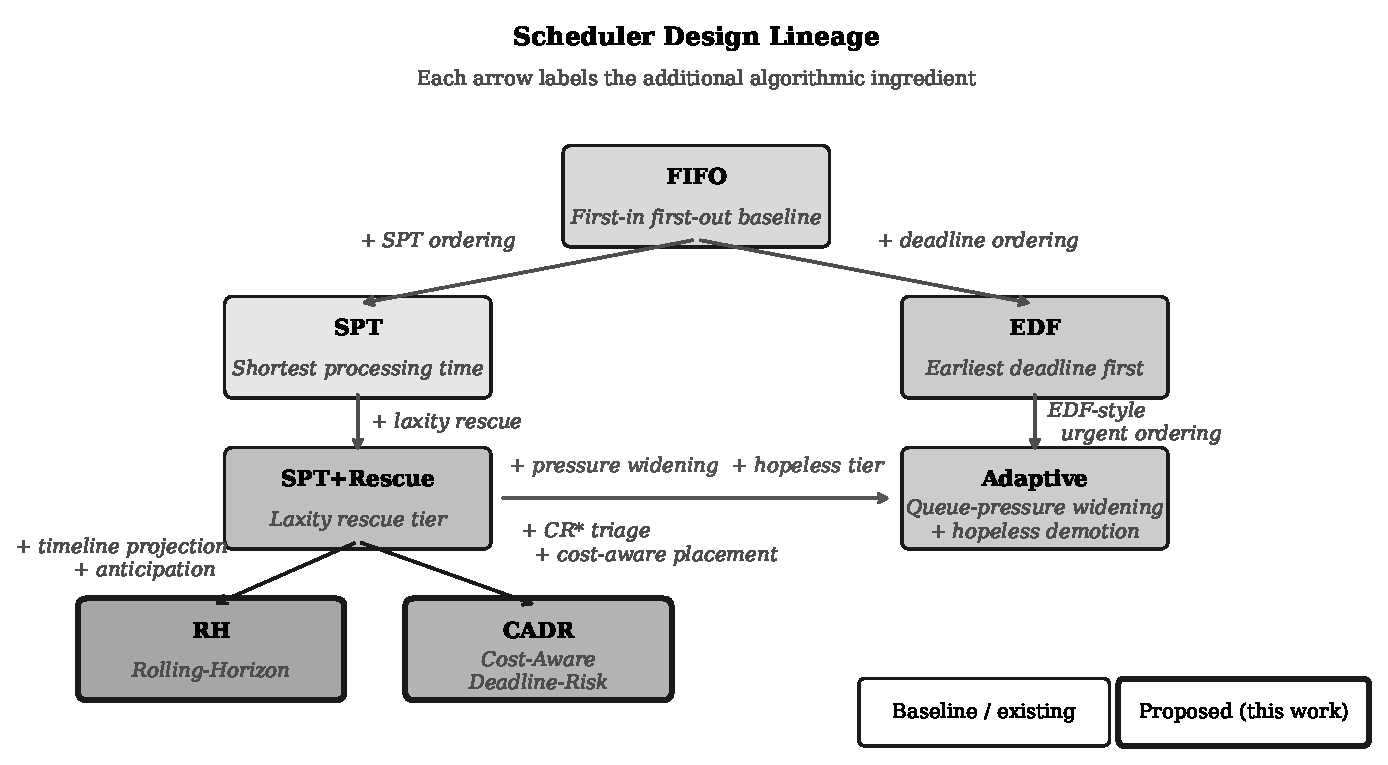
\includegraphics[width=0.98\linewidth,height=0.72\textheight,keepaspectratio]{figures/scheduler_lineage.pdf}
\caption[Scheduler design lineage]{Scheduler design lineage. Each arrow labels the algorithmic ingredient added at that step. FIFO is the deadline-oblivious baseline; SPT adds shortest-job-first ordering to reduce wait; EDF adds deadline ordering to reduce misses; SPT+Rescue adds a laxity rescue tier to combine both effects; the Adaptive hybrid extends the rescue tier with queue-pressure tier widening and hopeless demotion; the proposed RH scheduler replaces the hand-set slack threshold with a boundary read from a forward timeline projection and adds load-gated anticipation; the proposed CADR scheduler replaces the laxity threshold with a scale-free critical-ratio triage and adds cost-aware node selection.}
\label{fig:scheduler-lineage}
\end{figure}
\end{landscape}

\subsection{SPT+Rescue: Hybrid Throughput-Deadline Policy}
\label{ssec:spt-rescue-hybrid-throughput-deadline-policy}

SPT+Rescue introduces the laxity rescue concept as an intermediate design step. It combines SPT's wait-time advantage with an EDF-based deadline rescue mechanism: most jobs are ordered by shortest processing time, but any job whose \emph{laxity} drops below a threshold is promoted to an urgent tier and dispatched before all normal-tier jobs.

The laxity of job $j$ at scheduling decision time $t$ is defined as:
\begin{equation}
L_j(t) = d_j - t - \min_{m \in I}\, \overline{W}(\kappa_j, g(m))
\label{eq:laxity}
\end{equation}
where the minimum is taken over all currently idle nodes $I$. Laxity measures the slack remaining: if $L_j(t) < 0$, even immediate dispatch on the fastest idle node misses under the mean service-time estimate, but a shorter realised execution time can still meet the deadline; small positive laxity signals risk if dispatch is deferred.

At each scheduling event the scheduler partitions the waiting queue into two tiers (Figure~\ref{fig:rescue-flow}):
\begin{itemize}
  \item \textbf{Urgent} ($L_j < \theta$): sorted by earliest absolute deadline (EDF order within tier)
  \item \textbf{Normal} ($L_j \geq \theta$): sorted by shortest estimated processing time (SPT order)
\end{itemize}

\begin{landscape}
\begin{figure}[H]
\centering
\captionsetup{font=small,skip=6pt}
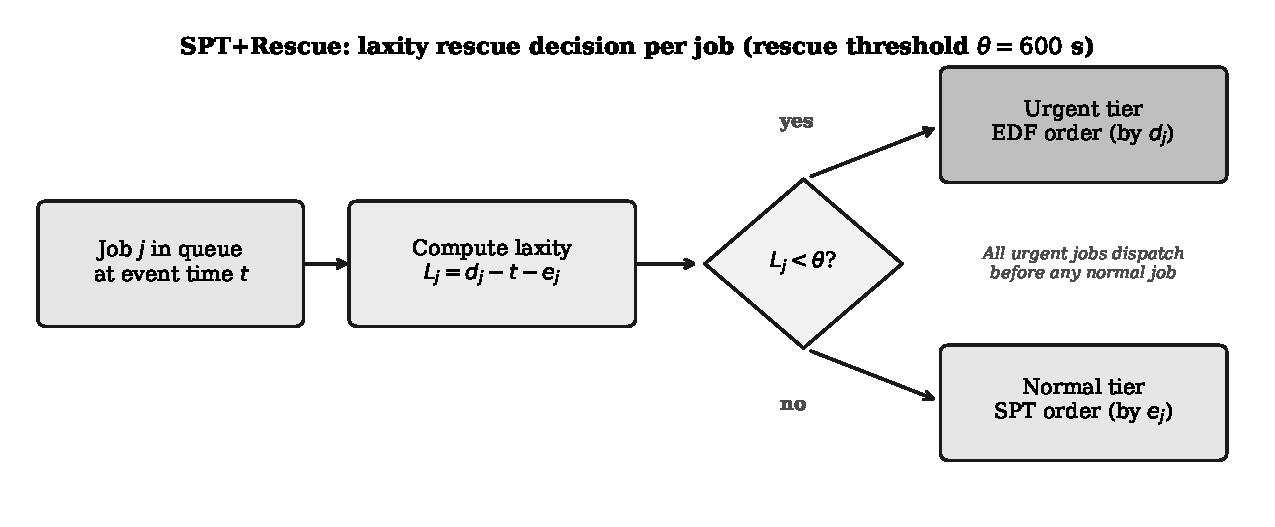
\includegraphics[width=0.98\linewidth,height=0.72\textheight,keepaspectratio]{figures/rescue_flow.pdf}
\caption[SPT+Rescue laxity rescue decision flow]{SPT+Rescue per-job decision flow. At each scheduling event, every queued job's laxity $L_j = d_j - t - e_j$ is computed against the fastest available execution time; jobs with laxity below the rescue threshold $\theta$ enter the urgent tier (EDF order), the rest stay in the normal tier (SPT order), and all urgent jobs dispatch before any normal job.}
\label{fig:rescue-flow}
\end{figure}
\end{landscape}
All urgent jobs are dispatched before any normal-tier job. The rescue threshold is set to $\theta = 600$\,s (10 minutes) in all experiments. This value was chosen by the following reasoning: by the laxity definition (Eq.~\ref{eq:laxity}), a job that has just crossed the rescue threshold has laxity exactly $\theta$, so dispatching it immediately leaves exactly $\theta = 600$\,s to spare before the deadline, comfortably above even a high-complexity job's empirical 99th-percentile render time (about 150\,s; the observed maximum is about 350\,s). The margin covers render-time variability and a High or Medium stock provisioning delay (at most 120\,s), but not a Low-stock delay (at least 600\,s), which the model can draw during peak hours. A sensitivity study over $\theta \in \{60, 180, 300, 600, 1200\}$\,s (Section~\ref{ssec:rescue-threshold-sensitivity}) ($n=10$ seeds) shows that miss rate varies by \ThrMissSpread\,percentage points across the whole swept range, a little over half of it from the shortest threshold: $\theta=60$\,s is the weakest, whereas the four values $\theta \ge 180$\,s lie within about two percentage points of each other, a spread comparable to the seed noise at this sample size. The sweep minimum lies at $\theta=180$\,s, so the default $\theta=600$\,s sits on the flat part of the curve and requires no tuning. Algorithm~\ref{alg:sptrescue} summarises the two-tier procedure.

\begin{algorithm}[H]
\caption{SPT+Rescue Scheduler}
\label{alg:sptrescue}
\begin{algorithmic}[1]
\REQUIRE Queue $Q$; idle node set $I$; current time $t$; threshold $\theta$
\FOR{each job $j \in Q$}
  \STATE $e_j \leftarrow \min_{m \in I} \overline{W}(\kappa_j, g(m))$ \COMMENT{fastest available expected exec time}
  \STATE $L_j \leftarrow d_j - t - e_j$
\ENDFOR
\STATE $Q_{\text{urgent}} \leftarrow \{j \in Q : L_j < \theta\}$, sorted by $d_j$ ascending
\STATE $Q_{\text{normal}} \leftarrow \{j \in Q : L_j \geq \theta\}$, sorted by $e_j$ ascending
\FOR{each job $j$ in $Q_{\text{urgent}} \mathbin{\|} Q_{\text{normal}}$}
  \IF{$I = \emptyset$} \STATE \textbf{break} \ENDIF
  \STATE $m^* \leftarrow \arg\min_{m \in I} \big[(1{-}w_c)\tfrac{\overline{W}(\kappa_j, g(m))}{\overline{W}_{\min}(j)} + w_c\tfrac{p_{g(m)}}{p_{\min}} + \text{sp}(s_m)\big]$ \COMMENT{Eq.~\ref{eq:spt_score}, $w_c{=}0.3$}
  \STATE Assign $j \to m^*$; remove $m^*$ from $I$
\ENDFOR
\end{algorithmic}
\end{algorithm}

SPT+Rescue combines SPT's shortest-job-first ordering with EDF deadline rescue: under capacity saturation it achieves \RescueMiss\% miss (notably lower than SPT's \SPTmiss\%) at \RescueWait~min wait ($d=\RescueFIFOwaitD$ vs FIFO, $p<0.001$), providing a conservative fallback when tight-deadline compliance is a strict operational requirement.

\subsection{Illustrative Scheduling Example}
\label{ssec:illustrative-scheduling-example}

Figure~\ref{fig:gantt} traces a concrete 7-job scenario with $C_{\max}=3$ nodes (a minimal illustrative configuration chosen so that all 7 jobs queue up and the rescue decision is visible; the baseline experiments use $C_{\max}=5$, and the concurrency sweep varies it) to show how SPT+Rescue differs from FIFO in a single scheduling window. Only J6 carries an illustrative tight deadline ($d_6=210$\,s, 160\,s after its arrival at $t=50$\,s; $\kappa_6=2$, medium complexity); this deliberately shortened window makes the rescue decision visible and is not the baseline one-hour tight window used in the experiments. All other jobs have loose (8-hour) deadlines. The illustrative scenario sets provisioning delay to zero and uses approximated, complexity-uniform execution times matching the figure legend ($\kappa{=}1\approx65$\,s, $\kappa{=}2\approx75$\,s, $\kappa{=}3\approx120$\,s, the last chosen for narrative clarity rather than as a close rounding of the empirical high-complexity mean). J0, J1, J2 arrive in the first 10\,s and fill all three nodes immediately; J3 to J6 queue while all nodes are busy. When node N1 becomes free at $t=70$\,s, FIFO dispatches J3 (next in arrival order), then at $t=75$\,s dispatches J4 to N2, eventually assigning J6 to N2 at $t=140$\,s. J6 finishes at 215\,s, 5\,s past its deadline ($\delta_6=0$). SPT+Rescue instead evaluates laxity when N1 frees at $t=70$\,s (the sole idle node at that moment; $\overline{W}(\kappa_6{=}2, g(\text{N1}))=75$\,s):
\begin{equation}
  L_{J_6}(70) = d_6 - 70 - \min_{m \in I} \overline{W}(\kappa_6, g(m)) = 210 - 70 - 75 = 65\,\text{s}
\end{equation}
Since $65$\,s is below the $600$\,s rescue threshold, J6 is classified urgent and dispatched immediately to N1. J6 starts at $t=70$\,s and finishes at 145\,s, meeting its deadline by 65\,s ($\delta_6=1$). Loose-deadline jobs J3 to J5 are reordered by SPT without any deadline impact.

\begin{landscape}
\begin{figure}[H]
\centering
\captionsetup{font=small,skip=6pt}
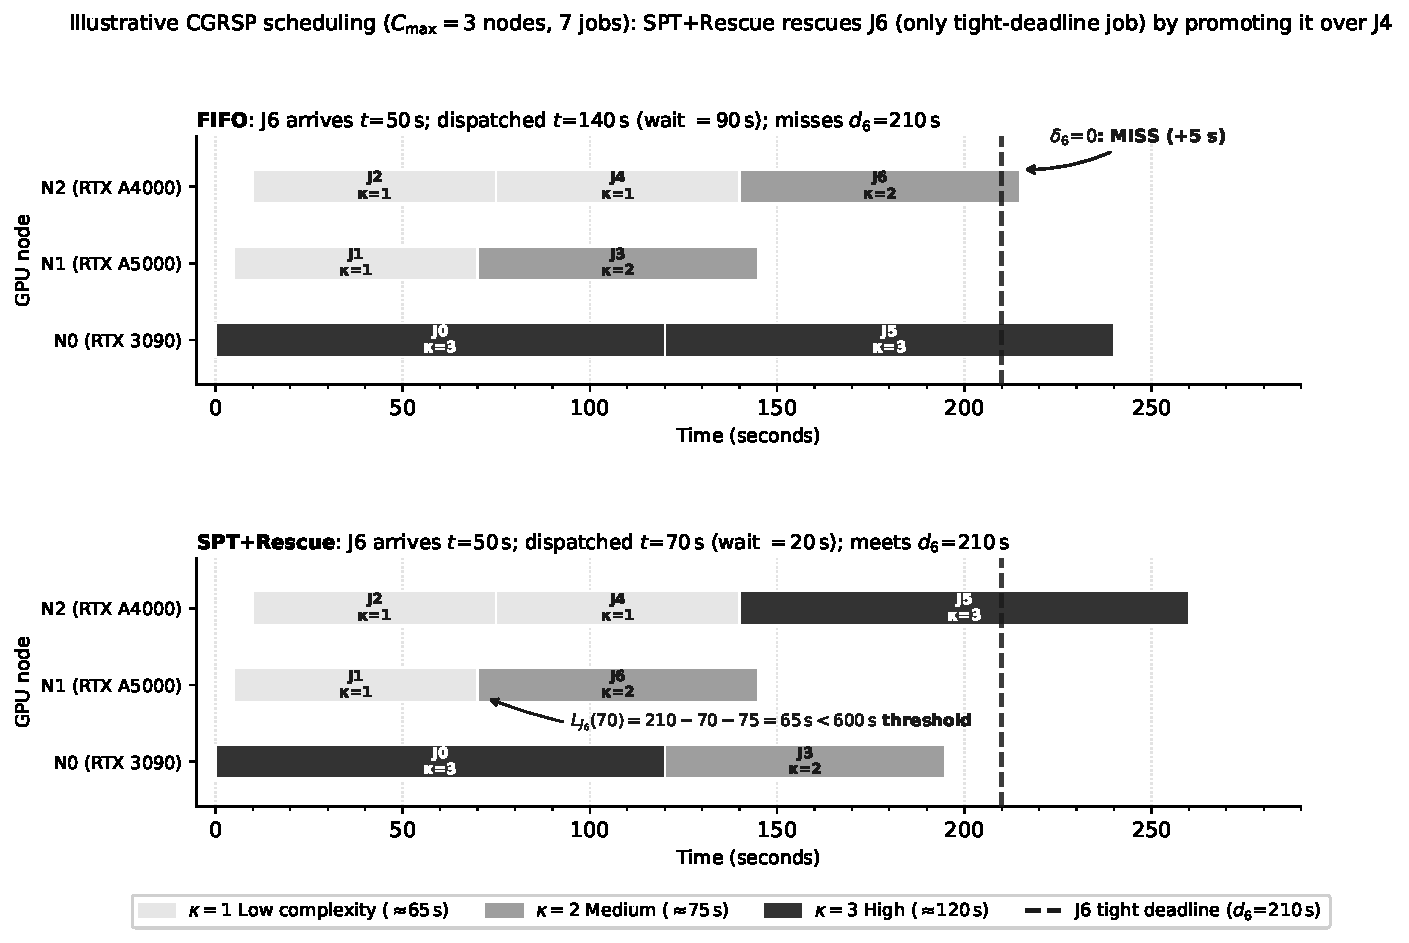
\includegraphics[width=0.98\linewidth,height=0.88\textheight,keepaspectratio]{figures/gantt_chart.pdf}
\caption[Illustrative Gantt chart: FIFO vs SPT+Rescue]{Illustrative Gantt chart: FIFO vs SPT+Rescue.}
\label{fig:gantt}
\end{figure}
\end{landscape}


\subsection{Anticipative Rolling-Horizon Scheduler}
\label{ssec:anticipative-rolling-horizon-scheduler}

The Rolling-Horizon (RH) scheduler is the first, and methodologically the more novel, of the two scheduling contributions of this work. Rather than ranking the queue by a single fixed priority rule, it projects the near-future availability of the fleet and dispatches against that projection. At each scheduling event it builds the availability timeline of every usable slot (idle now, or busy until its running job's expected completion), classifies each waiting job by whether the timeline shows it would still meet its deadline if it deferred to the next slot to free, and then greedily places jobs, in that urgency order, each onto the slot that minimises a per-job weighted-sum surrogate of the model objective (Eq.~\ref{eq:objective}), namely the projected value, under the planning estimate $e_j$ in place of the realised $W$, of $w_{\text{qos}}(\alpha_1 w_j + \alpha_2 (1-\delta_j)) + w_{\text{cost}}\,c_j$ with $w_{\text{qos}}=w_{\text{cost}}=0.5$ (the explicit form is given in Algorithm~\ref{alg:rh}). The score additionally includes a stock-status penalty and a fixed per-type reliability prior. Thus a tie in projected QoS does not guarantee that the lowest-cost node wins; this is a heuristic approximation of, not an exact solution to, the lexicographic objective. It commits only the dispatches that start at the current instant and re-plans at the next event, in the manner of receding-horizon (model-predictive) control. The placement step is a greedy, per-job assignment rather than a joint optimisation over the horizon; the tier orders themselves are fixed rules (shortest processing time first for normal jobs, earliest deadline first for urgent jobs, doomed jobs last), and what is novel is that the boundary between the urgent and normal tiers is read from the projected slot timeline, adapting to the realised fleet state, instead of from a hand-set laxity threshold. The scheduler is additionally anticipative: below saturation it reserves a little capacity for imminent tight-deadline arrivals (described below).

The RH scheduler is anticipative but not clairvoyant: it knows the job arrival-rate profile and the deadline-window distribution (operational statistics estimable from a studio's own submission history), but it does not observe the identities or submission times of jobs that have not yet arrived. This is the standard distinction in online stochastic optimisation between distributional knowledge and realisation knowledge: the scheduler may reserve capacity for the \emph{expected} rate of imminent tight-deadline arrivals, never for specific future jobs.

That the arrival rate is estimable in principle does not make the policy indifferent to how well it is estimated, and the sensitivity has an unusual shape that a practitioner needs to know about. The assumed $\lambda$ enters the policy at exactly one place, the load gate of the anticipation mechanism described below, and the gate is a step function: it compares $\rho = \lambda\,\overline{W}/C_{\max}$ against $\rho_{\text{gate}}$, which at $C_{\max}=5$ puts the switching point at $\lambda \approx \PriorGateLambda$~jobs/s, only about \PriorGateShortfall\% below the hectic day's true rate of $0.100$~jobs/s. A 30-seed sweep in which RH is given a deliberately mis-estimated arrival rate, swept as a multiple of the true $\lambda$ on the hectic and surge days, confirms both halves of this shape. On the hectic day, mis-estimates that leave the assumed $\lambda$ on the correct side of the switching point change nothing at all, reproducing the gated result of \RHMiss\% miss at \RHWait~min wait exactly; but an under-estimate large enough to cross the point wrongly convinces the scheduler there is spare capacity to hold back, so it reserves a slot in a saturated queue. Miss then more than doubles, and mean wait rises well above FIFO's \FIFOwait~min ($p<0.001$, paired against FIFO on the same seeds), which is the practically important failure: a studio that under-estimates its own peak load turns the anticipation mechanism from inert into actively harmful. Two qualifications keep this in proportion. Even in that degraded state RH's miss rate remains significantly \emph{below} FIFO's \FIFOmiss\% ($p<0.001$), so the policy is not dominated by the baseline; the damage is concentrated in wait. And the exposure is one-sided by day type: on the surge day, whose true rate sits far below the switching point, every under-estimate and moderate over-estimate is inert, and only a large over-estimate crosses the point (it lies at about \PriorSurgeCrossX{} times the true rate; the sweep's twofold over-estimate is inert and its fourfold one crosses), switching anticipation off and raising miss from \ResSurgeOnMiss\% to \ResSurgeOffMiss\%. The practical guidance is therefore not that $\lambda$ must be known precisely, but that it must be known well enough to place the busiest day on the correct side of $\rho_{\text{gate}}$; a deliberately conservative (high) estimate fails safe on saturated days, at the cost of forgoing anticipation on quiet ones.

\textbf{Slot timelines.} Each of the $C_{\max}$ slots is modelled as an availability timeline. An idle slot is free from the current time $t$; a running slot is busy until its dispatch time plus the mean service time $e_j$ (the provisioning delay is not known at dispatch and is not included, so the projection is optimistic by $\tau^{\text{prov}}_j$). Every slot is either idle or running under the on-demand pool, so the timeline spans all $C_{\max}$ slots. When every slot is idle, $t_{\text{free}}$ has no busy slot to derive from and is approximated as the completion time of a hypothetical medium-complexity job started now; this affects the urgent/normal boundary only in the fully idle fleet state. Two further implementation details qualify the picture. Only idle slots are placement candidates; a running slot enters the plan solely through its expected free time, which sets $t_{\text{free}}$. Each job is planned onto an idle slot's timeline at its earliest feasible start, so a job may be planned at a later start behind an earlier-ordered placement on the same slot, and these deferred placements occupy the timelines against which later-ordered jobs are placed, but only placements that start now are committed, and the rest of the plan is discarded and rebuilt at the next event. And the projection is certainty-equivalent: a running slot whose realised (log-normal) service time has already exceeded its planned mean, or whose provisioning delay has consumed the planned window, is projected to free immediately, so at such decision events $t_{\text{free}}$ collapses to the current instant, the urgent tier empties, and the realised ordering reduces to SPT with hopeless-job demotion. In an instrumented run of the baseline hectic day (seeds 0 to 2; \texttt{CGRSP/phase3\_diagnostics.py}), $t_{\text{free}}$ collapsed to the current instant at about \TFreeCollapsedPct\% of the decision events with at least one busy slot; the saturated-regime miss advantage therefore rests chiefly on doomed-job demotion (the RH-over-SPT+Rescue ablation step), with the EDF-style urgent tier contributing in partially loaded and below-saturation states.

\textbf{Candidate ordering.} For each waiting job the scheduler computes the expected service time $e_j = \min_{m} \overline{W}(\kappa_j, g(m))$ over idle capable slots and classifies it against the soonest time a slot would free for a job not dispatched now, $t_{\text{free}}$ (Figure~\ref{fig:rh-timeline}):
\begin{itemize}
  \item \textbf{Urgent}: $t + e_j \leq d_j < t_{\text{free}} + e_j$. Projected to meet its deadline only if dispatched now. Ordered by earliest deadline (EDF).
  \item \textbf{Normal}: $t_{\text{free}} + e_j \leq d_j$. Projected to finish in time even after waiting for the next slot. Ordered by shortest $e_j$ (SPT), which targets lower mean wait.
  \item \textbf{Hopeless under the planning estimate}: $t + e_j > d_j$. Even immediate dispatch is projected to miss; a shorter realised service time can still meet the deadline. Ordered last.
\end{itemize}
Demoting jobs projected to miss under the mean-service estimate can leave capacity for jobs projected to meet their deadlines. Because realised service and provisioning are stochastic, this heuristic can also demote a job that could still finish on time; it is not guaranteed to minimise the binary miss count.



\noindent\textit{Figure~\ref{fig:rh-timeline} notes.} Rolling-Horizon slot timelines and job classification at a single scheduling event. Top: the fleet's availability timeline; Slot~1 is idle now, Slot~2 frees at $t_{\rm free}$ (the soonest time a slot becomes available for a job not dispatched now), Slot~3 frees later. Bottom: three waiting jobs, each shown with its execution window if dispatched now (solid bar) and if deferred to $t_{\rm free}$ (dashed outline) against its deadline (black marker). Job~A is projected to meet its deadline only if dispatched now (Urgent); Job~B is projected to finish in time after deferring (Normal); Job~C is projected to miss even with immediate dispatch (Hopeless tier, dispatched last under the mean-service estimate; a shorter realisation may still meet its deadline).\par

\textbf{Anticipation (load-gated reservation).} Below saturation the scheduler reserves a small amount of idle capacity for anticipated tight-deadline (rush-order) arrivals rather than spending it on loose jobs that have ample slack, and it dispatches waiting tight jobs eagerly so that a held slot is actually taken by the rush job it was kept for. (The implementation classifies a job as tight when its deadline window is below 7{,}200\,s, twice $T_{\text{tight}}$; under the baseline \{3600, 28800\}\,s windows this selects exactly the tight class.) The reservation count $\rho_{\text{res}}$ sets how many idle slots are held back ($\rho_{\text{res}}=1$ by default); tight jobs may always use any idle slot, and only loose jobs are withheld, so deadline-critical work is never starved of capacity. The mechanism is gated by the offered load $\rho = \lambda\,\overline{W}/C_{\max}$, computed from the known arrival-rate profile $\lambda$ (distributional knowledge only, as above) and the mean service time $\overline{W}$: when $\rho \geq \rho_{\text{gate}}$ (here $0.95$) the system is saturated, every slot is needed immediately, and reservation is disabled (any $\rho_{\text{res}}$ reduces to the plain forward-simulation policy); when $\rho < \rho_{\text{gate}}$ there is execution capacity to spare (the gate does not count the provisioning delay for which a dispatch also holds its slot). This is the operational meaning of anticipation being self-limiting: it activates exactly when reserving a slot for an imminent tight arrival does not delay a job that cannot wait. Section~\ref{ssec:anticipation-reservation-sensitivity} shows that load-gated anticipation substantially reduces tight-deadline miss below saturation (the surge day) while the gate correctly switches it off under saturation (the hectic day), where reserving capacity would only delay jobs that cannot be deferred. The baseline hectic-day results ($C_{\max}=5$) are therefore produced by the plain forward-simulation policy and are unaffected by anticipation; in the $C_{\max}$ sensitivity runs at 7 and 10 slots the offered load falls below the gate and anticipation is active. The monthly results are not: of the four day types in the Phase~4 calendar only the hectic day exceeds the gate, so reservation is live on the surge, normal and quiet days, which together are the large majority of simulated days. Re-running the whole month with reservation disabled, on the identical schedules and per-day seeds, raises the monthly deadline-miss rate and mean tardiness significantly ($p<0.001$ on each, paired over the monthly replications) while reducing mean wait slightly (\MonthResWaitP, uncorrected; these paired tests are reported separately from the Phase~3 family), the same wait-for-miss trade the surge-day sweep shows in isolation. The monthly headline is thus an anticipation-enabled result, not a plain forward-simulation one; the reservation-disabled arm is retained as a reported comparison arm in the Phase~4 results file, and the shipped RH configuration is unchanged by it.

\textbf{Node selection.} Within a placement the GPU type is chosen by minimising the bi-objective contribution (expected wait and miss penalty, plus operational cost), with a stock-status penalty derived from $s_g(t)$ and a fixed per-type reliability prior (RTX~A4000 0, A4500 0.05, A5000 0.15, 3090 0.40) whose ordering mirrors the baseline high-stock probabilities $\beta_g$. Because the wait and miss terms are identical across idle-now slots and the per-job cost term is small at this fleet scale, this prior is the deciding term among idle slots in practice: RH systematically prefers the types the calibration assumes to be better stocked (the higher-$\beta_g$ types, which are also the cheaper ones; $\beta_g$ is a modelling assumption, Section~\ref{ssec:platform-and-data}, and the snapshot record's per-type offer shares rank the types the other way, Section~\ref{ssec:availability-model-sensitivity}) unless the deadline term forces a faster GPU. Secondary ordering tiebreakers (deadline then service time in the urgent and hopeless tiers, service time then deadline in the normal tier) are applied as documented in the implementation.

\begin{algorithm}[H]
\caption{Rolling-Horizon Scheduler}
\label{alg:rh}
\begin{algorithmic}[1]
\REQUIRE Queue $Q$; usable slots $S$ (placement candidates are the idle slots; running slots enter only through their expected free time, which sets $t_{\text{free}}$); time $t$; arrival rate $\lambda$; reservation $\rho_{\text{res}}$; gate $\rho_{\text{gate}}$
\STATE $\rho \leftarrow \lambda\,\overline{W}/C_{\max}$; \quad $R \leftarrow \rho_{\text{res}}$ if $\rho < \rho_{\text{gate}}$ else $0$ \COMMENT{load gate: reserve only below saturation}
\STATE build slot timelines from $S$; $t_{\text{free}} \leftarrow$ soonest time a slot frees for a non-dispatched job
\FOR{each job $j \in Q$}
  \STATE $e_j \leftarrow \min_{m} \overline{W}(\kappa_j, g(m))$ over idle capable slots
\ENDFOR
\STATE order $Q$: hopeless ($t+e_j > d_j$) last; else if $R>0$ and $j$ tight, urgent (by $d_j$, eager); else urgent ($t_{\text{free}}+e_j > d_j$, by $d_j$); else normal (by $e_j$)
\FOR{each candidate $j$ in order}
  \STATE place $j$ at its earliest feasible start minimising the projected $w_{\text{qos}}(\alpha_1 w_j + \alpha_2 (1-\delta_j)) + w_{\text{cost}} c_j$ (under the planning estimate $e_j$) plus stock-status penalty and fixed per-type reliability prior
\ENDFOR
\STATE commit each job whose placement starts at $t$ on an idle slot
\STATE \textbf{if} $R>0$: withhold loose-job commits so $R$ idle slots stay free for tight arrivals
\STATE discard uncommitted placements and re-plan at the next event
\end{algorithmic}
\end{algorithm}

\begin{landscape}
\begin{figure}[H]
\centering
\captionsetup{font=small,skip=6pt}
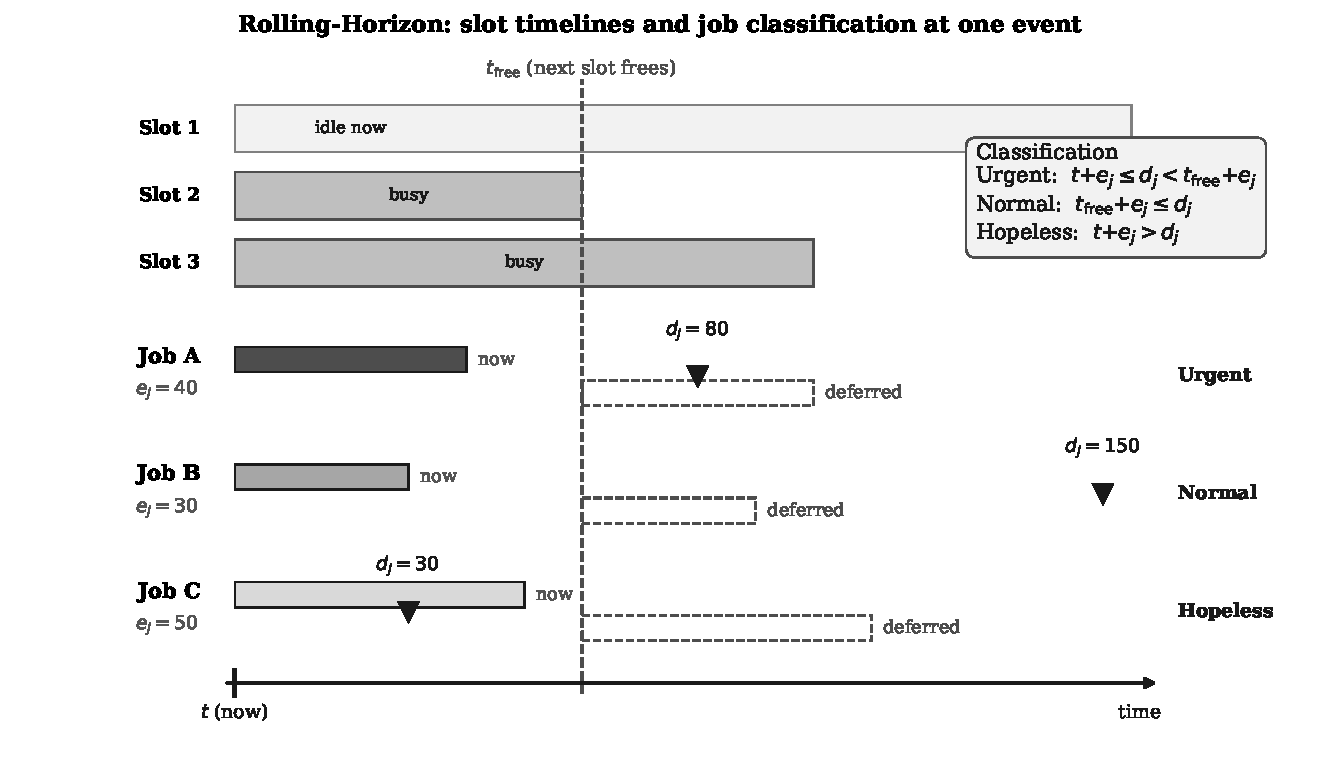
\includegraphics[width=0.98\linewidth,height=0.90\textheight,keepaspectratio]{figures/rh_timeline.pdf}
\caption[Rolling-Horizon slot timelines and job classification]{Rolling-Horizon slot timelines and job classification.}
\label{fig:rh-timeline}
\end{figure}
\end{landscape}

The RH scheduler is implemented in \texttt{CGRSP/\allowbreak cgrsp/\allowbreak schedulers/\allowbreak rolling\allowbreak\_horizon\allowbreak\_scheduler.py}. Anticipation is enabled ($\rho_{\text{res}}=1$, load-gated) in all experiments; because the gate disables it under saturation, the baseline hectic-day results ($C_{\max}=5$) are identical to the plain forward-simulation policy (at $C_{\max}\ge 8$ the offered load falls below the gate and anticipation is active), while the surge day exhibits its benefit and the monthly results, whose calendar is mostly below the gate, carry it throughout. The reservation count and the gate are examined in Section~\ref{ssec:anticipation-reservation-sensitivity}.

\subsection{CADR: Cost-Aware Deadline-Risk}
\label{ssec:cadr-cost-aware-deadline-risk}

The Cost-Aware Deadline-Risk (CADR) scheduler is the second scheduling contribution of this work. Like RH, CADR classifies waiting jobs into tiers based on deadline urgency; unlike RH, it uses a scale-free critical ratio rather than a forward-simulation timeline, and it integrates cost-aware node selection as a secondary objective.

\textbf{Critical ratio.} The critical ratio is a classical dispatching rule from the operations-research literature~\cite{pinedo2016scheduling}; the contribution here is its combination with the scale-free three-tier triage, doomed-last demotion, and stock-filtered cheapest-deadline-feasible placement. For each job $j$ at scheduling time $t$ with estimated service time $e_j = \min_{m \in I} \overline{W}(\kappa_j, g(m))$, the critical ratio is:
\begin{equation}
\mathrm{CR}_j(t) = \frac{d_j - t}{e_j}
\label{eq:cr}
\end{equation}
A ratio $\mathrm{CR}_j \leq 1$ means the remaining time is at most the estimated service time, so immediate dispatch leaves no estimated slack for provisioning; a shorter realised service time may still meet the deadline. Such jobs enter the last tier. $\mathrm{CR}_j = \mathrm{CR}^*$ is the boundary between at-risk and safe jobs, with a baseline $\mathrm{CR}^* = 3$.

\textbf{Three-tier classification.} At each scheduling event the waiting queue is partitioned by the critical ratio (Eq.~\ref{eq:cr}) into three tiers (Figure~\ref{fig:cadr-triage}a):
\begin{itemize}
  \item \textbf{Doomed under the estimate} ($\mathrm{CR}_j \leq 1$): immediate dispatch is projected to miss; dispatched \emph{last} to prioritise jobs projected to meet their deadlines.
  \item \textbf{At-risk} ($1 < \mathrm{CR}_j \leq \mathrm{CR}^*$): deadline is reachable but slack is tight; dispatched in earliest-deadline-first (EDF) order.
  \item \textbf{Safe} ($\mathrm{CR}_j > \mathrm{CR}^*$): ample slack remaining; dispatched in shortest-processing-time (SPT) order to minimise mean wait.
\end{itemize}

\textbf{Cost-aware node selection.} Within a placement (Figure~\ref{fig:cadr-triage}b), CADR first restricts the capable nodes to those not currently low on stock (falling back to all capable nodes only when every capable node is low-stock, since low stock signals a longer expected provisioning delay), then selects the cheapest among them whose estimated finish time satisfies the deadline (deadline-feasible cheapest node). If no deadline-feasible node exists, it falls back to the fastest node in the same stock-filtered pool. This integrates cost awareness directly into dispatch rather than as a post-hoc re-scoring.



\textbf{Why CADR has lower tardiness than RH.} Both schedulers demote on an instantaneous test (RH: $t + e_j > d_j$; CADR: $\mathrm{CR}_j \leq 1$), and both dispatch demoted jobs last in deadline order. Because both take $e_j$ over the idle slots and RH's strict test $t + e_j > d_j$ implies $\mathrm{CR}_j \leq 1$, any job RH demotes at a given instant CADR demotes too, so the difference does not lie in demotion. It lies in promotion. Under saturation RH moves a job into its urgent tier only when it can no longer wait for the next slot to free ($t_{\text{free}} + e_j > d_j$), a window of roughly one service time that is planned without the provisioning delay. A tight job not dispatched inside that window becomes hopeless and waits behind the loose backlog, so RH's missed jobs are frequently tight jobs that finish hours late. CADR's at-risk tier opens at $\mathrm{CR}_j \leq \mathrm{CR}^* = 3$, about three service times before the deadline, so tight jobs are dispatched with margin, and its missed jobs are almost all loose jobs that finish modestly late. As a result, CADR gives substantially lower mean tardiness than RH while keeping the miss count nearly as low.

\textbf{Ablation variant.} The CADR-order-only (CADR-OO) variant retains the three-tier critical-ratio ordering but replaces cost-aware node selection with fastest-available-node placement within the stock-filtered pool. This isolates the contribution of the cost-aware placement component from the ordering component (Section~\ref{sec:ablation-analysis}).

\begin{algorithm}[H]
\caption{CADR Scheduler}
\label{alg:cadr}
\begin{algorithmic}[1]
\REQUIRE Queue $Q$; idle node set $I$; current time $t$; threshold $\mathrm{CR}^*=3$
\FOR{each job $j \in Q$}
  \STATE $e_j \leftarrow \min_{m \in I} \overline{W}(\kappa_j, g(m))$
  \STATE $\mathrm{CR}_j \leftarrow (d_j - t) / e_j$
\ENDFOR
\STATE $Q_{\text{doomed}} \leftarrow \{j \in Q : \mathrm{CR}_j \leq 1\}$, ordered last
\STATE $Q_{\text{atrisk}} \leftarrow \{j \in Q : 1 < \mathrm{CR}_j \leq \mathrm{CR}^*\}$, sorted by $d_j$ ascending (EDF)
\STATE $Q_{\text{safe}}   \leftarrow \{j \in Q : \mathrm{CR}_j > \mathrm{CR}^*\}$, sorted by $e_j$ ascending (SPT)
\FOR{each job $j$ in $Q_{\text{atrisk}} \mathbin{\|} Q_{\text{safe}} \mathbin{\|} Q_{\text{doomed}}$}
  \IF{$I = \emptyset$} \STATE \textbf{break} \ENDIF
  \STATE $I' \leftarrow \{m \in I : s_{g(m)}(t) \neq \text{Low}\}$; \quad \textbf{if} $I' = \emptyset$ \textbf{then} $I' \leftarrow I$ \COMMENT{stock-filtered pool}
  \STATE $I_{\text{feasible}} \leftarrow \{m \in I' : t + \overline{W}(\kappa_j, g(m)) \leq d_j\}$ \COMMENT{deadline-feasible nodes}
  \IF{$I_{\text{feasible}} \neq \emptyset$}
    \STATE $m^* \leftarrow \arg\min_{m \in I_{\text{feasible}}} p_{g(m)}$ \COMMENT{cheapest per-second rate, ties by exec time}
  \ELSE
    \STATE $m^* \leftarrow \arg\min_{m \in I'} \overline{W}(\kappa_j, g(m))$ \COMMENT{fastest fallback in the stock-filtered pool}
  \ENDIF
  \STATE Assign $j \to m^*$; remove $m^*$ from $I$
\ENDFOR
\end{algorithmic}
\end{algorithm}

\begin{landscape}
\begin{figure}[H]
\centering
\captionsetup{font=small,skip=6pt}
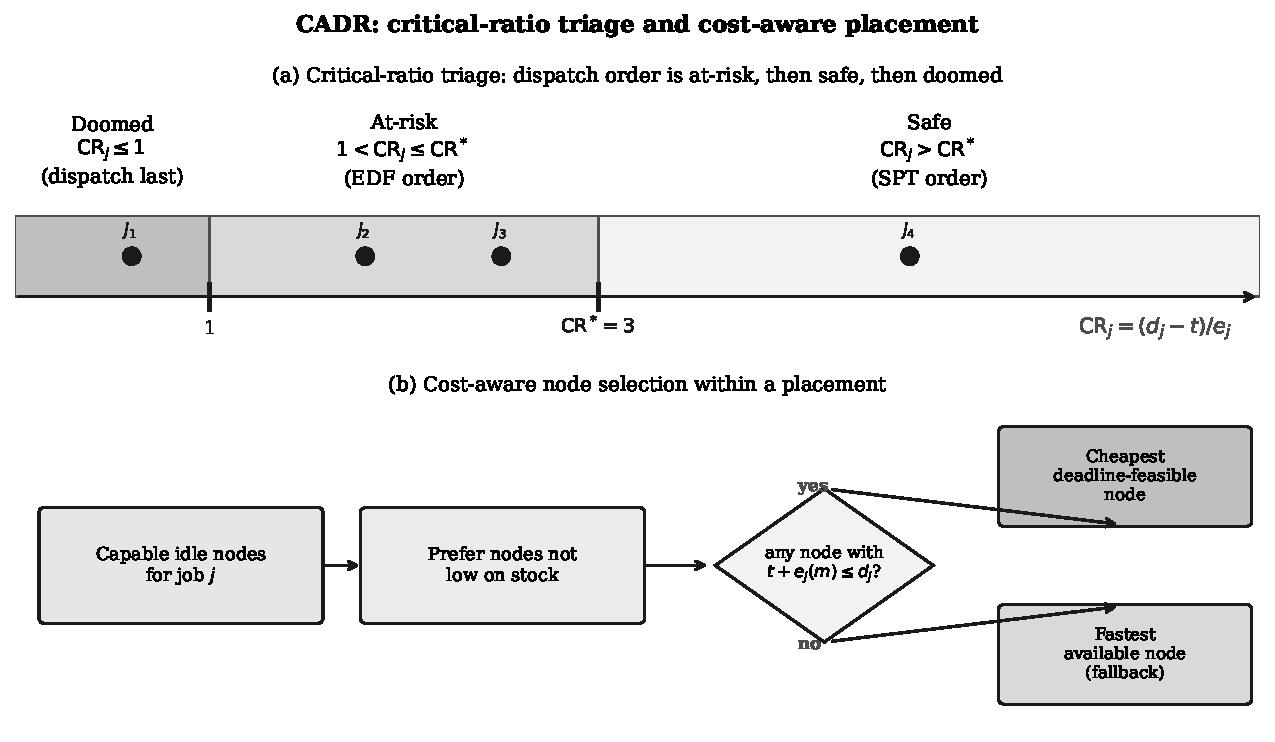
\includegraphics[width=0.98\linewidth,height=0.72\textheight,keepaspectratio]{figures/cadr_triage.pdf}
\caption[CADR critical-ratio triage and cost-aware placement]{CADR scheduling mechanics. Panel~(a): the critical ratio $\mathrm{CR}_j = (d_j - t)/e_j$ places every queued job on a scale-free axis partitioned into three tiers: doomed ($\mathrm{CR}_j \leq 1$, dispatched last), at-risk ($1 < \mathrm{CR}_j \leq \mathrm{CR}^*$, EDF order), and safe ($\mathrm{CR}_j > \mathrm{CR}^*$, SPT order); example jobs $j_1$ to $j_4$ illustrate the triage. Panel~(b): within each placement, node selection prefers non-low-stock nodes and picks the cheapest deadline-feasible node, falling back to the fastest available node when no node can meet the deadline.}
\label{fig:cadr-triage}
\end{figure}
\end{landscape}

Algorithm~\ref{alg:cadr} summarises the full procedure; the implementation is in \texttt{CGRSP/\allowbreak cgrsp/\allowbreak schedulers/\allowbreak cost\allowbreak\_aware\allowbreak\_deadline\allowbreak\_risk.py}. The critical-ratio threshold $\mathrm{CR}^*=3$ is the baseline; its sensitivity is examined in Section~\ref{ssec:critical-ratio-threshold-sensitivity}.

\subsection{Adaptive: Queue-Pressure EDF-SPT Hybrid}
\label{ssec:adaptive-queue-pressure-edf-spt-hybrid}

The Adaptive scheduler is a third hybrid policy, evaluated alongside RH and CADR to test the alternative ``adaptive SPT-EDF hybrid'' design. Like SPT+Rescue it uses a laxity threshold to separate urgent from non-urgent jobs, but it adds two refinements: a \emph{hopeless} tier that demotes jobs projected to miss under the service-time estimate (as in RH and CADR), and a \emph{queue-pressure} rule that widens the urgent tier as the backlog grows, so the policy interpolates between SPT under light load and EDF under heavy load.

At each scheduling event the laxity of job $j$ is computed exactly as in SPT+Rescue (Eq.~\ref{eq:laxity}), $L_j(t) = d_j - t - \min_{m \in I} \overline{W}(\kappa_j, g(m))$, and the queue is partitioned into three tiers against an \emph{effective} threshold $\theta_{\text{eff}}$:
\begin{itemize}
  \item \textbf{Critical} ($0 \leq L_j < \theta_{\text{eff}}$): dispatched first, in earliest-deadline (EDF) order.
  \item \textbf{Safe} ($L_j \geq \theta_{\text{eff}}$): dispatched next, in shortest-processing-time (SPT) order.
  \item \textbf{Hopeless under the estimate} ($L_j < 0$): projected to miss even if dispatched now; dispatched last (EDF order within the tier) to prioritise work projected to meet its deadline.
\end{itemize}
The queue-pressure adaptation sets $\theta_{\text{eff}} = \theta$ (baseline $600$\,s) under normal load, but expands it to the full loose-deadline window ($\theta_{\text{eff}} = T_{\text{loose}} = 28{,}800$\,s, a fixed constant in the implementation) whenever the waiting queue exceeds a pressure threshold $P$ (baseline $10$ jobs). Under that expansion every job with positive laxity falls into the critical tier, so the policy reduces to EDF ordering with hopeless-demotion exactly when the system is congested, the regime in which deadline ordering is most valuable; when the backlog is short it behaves as SPT for the safe majority. Critical-tier jobs are placed on the fastest deadline-reliable node (with a stock and provisioning-reliability penalty), while safe-tier jobs use the same speed-weighted cost-aware node score as SPT (Eq.~\ref{eq:spt_score}).

\begin{algorithm}[H]
\caption{Adaptive EDF-SPT Hybrid Scheduler}
\label{alg:adaptive}
\begin{algorithmic}[1]
\REQUIRE Queue $Q$; idle node set $I$; current time $t$; threshold $\theta$; pressure $P$
\STATE $\theta_{\text{eff}} \leftarrow T_{\text{loose}}$ \textbf{if} $|Q| > P$ \textbf{else} $\theta$ \COMMENT{queue-pressure widening}
\FOR{each job $j \in Q$}
  \STATE $e_j \leftarrow \min_{m \in I} \overline{W}(\kappa_j, g(m))$; \quad $L_j \leftarrow d_j - t - e_j$
\ENDFOR
\STATE $Q_{\text{crit}} \leftarrow \{j : 0 \leq L_j < \theta_{\text{eff}}\}$ sorted by $d_j$ (EDF)
\STATE $Q_{\text{safe}} \leftarrow \{j : L_j \geq \theta_{\text{eff}}\}$ sorted by $e_j$ (SPT)
\STATE $Q_{\text{hope}} \leftarrow \{j : L_j < 0\}$ sorted by $d_j$, ordered last
\FOR{each job $j$ in $Q_{\text{crit}} \mathbin{\|} Q_{\text{safe}} \mathbin{\|} Q_{\text{hope}}$}
  \IF{$I = \emptyset$} \STATE \textbf{break} \ENDIF
  \STATE $m^* \leftarrow$ fastest reliable node if $j$ critical (exec time plus stock penalty $\{0, 50, 200\}$\,s and per-type reliability prior $\{$A4000 0, A4500 5, A5000 15, 3090 40$\}$\,s), else speed-weighted cost-aware node (Eq.~\ref{eq:spt_score})
  \STATE Assign $j \to m^*$; remove $m^*$ from $I$
\ENDFOR
\end{algorithmic}
\end{algorithm}

Algorithm~\ref{alg:adaptive} summarises the procedure; the implementation is in \texttt{CGRSP/\allowbreak cgrsp/\allowbreak schedulers/\allowbreak adaptive\allowbreak\_scheduler.py}. It differs from RH in that its tier boundary is driven by an instantaneous laxity-and-queue-length rule rather than a forward-simulation timeline, and from CADR in that it uses an absolute laxity threshold rather than a scale-free critical ratio. Its empirical behaviour relative to RH and CADR is reported in Chapter~\ref{chap:experiments}.

\subsection{Ten-Policy Decision Snapshot}
\label{ssec:ten-policy-decision-snapshot}

Figure~\ref{fig:snapshot-decision} makes the decision-level difference concrete. It freezes one queue and fleet state at $t=600$\,s and presents it unchanged to all ten schedulers. Nine jobs wait; three slots are idle (A4000 and A4500 at High stock, A5000 at Medium) and two are busy (RTX~3090 and A4000). Under the mean service-time estimate on the fastest idle node, J1 and J8 can still meet their deadlines, J2 and J7 cannot even if dispatched immediately, and J3 to J6 and J9 have loose deadlines. The snapshot is illustrative, not a simulation result: it uses the same execution-time model and scheduler code as the experiments, but it is a single hand-chosen state.

FIFO, LCF and Balanced fill the three slots with loose jobs (J3 to J5), ignoring deadline risk. SPT serves J8 but spends the other two slots on loose jobs J3 and J6. EDF and SPT+Rescue dispatch J7 and J2, both already infeasible under the estimate, before J8: their urgent tier sorts by deadline, so the two earliest deadlines consume two slots even though neither job can be saved under the estimate. Random sends J7, J8 and J4. Adaptive, RH and CADR all leave J2 and J7 queued, dispatch both feasible tight jobs J1 and J8, and give the third slot to a loose job.

The difference is not node choice: all three idle slots are deadline-feasible for the feasible tight jobs, and the three policies that serve both differ only in which type receives which job. The gain comes from the ordering: not spending capacity on jobs that cannot meet their deadlines, and promoting the two feasible tight jobs. This is the mechanism behind the aggregate miss differences in Chapter~\ref{chap:experiments}; the snapshot shows why deadline-aware demotion matters, not that any one policy wins on every event.

\begin{figure}[H]
\centering
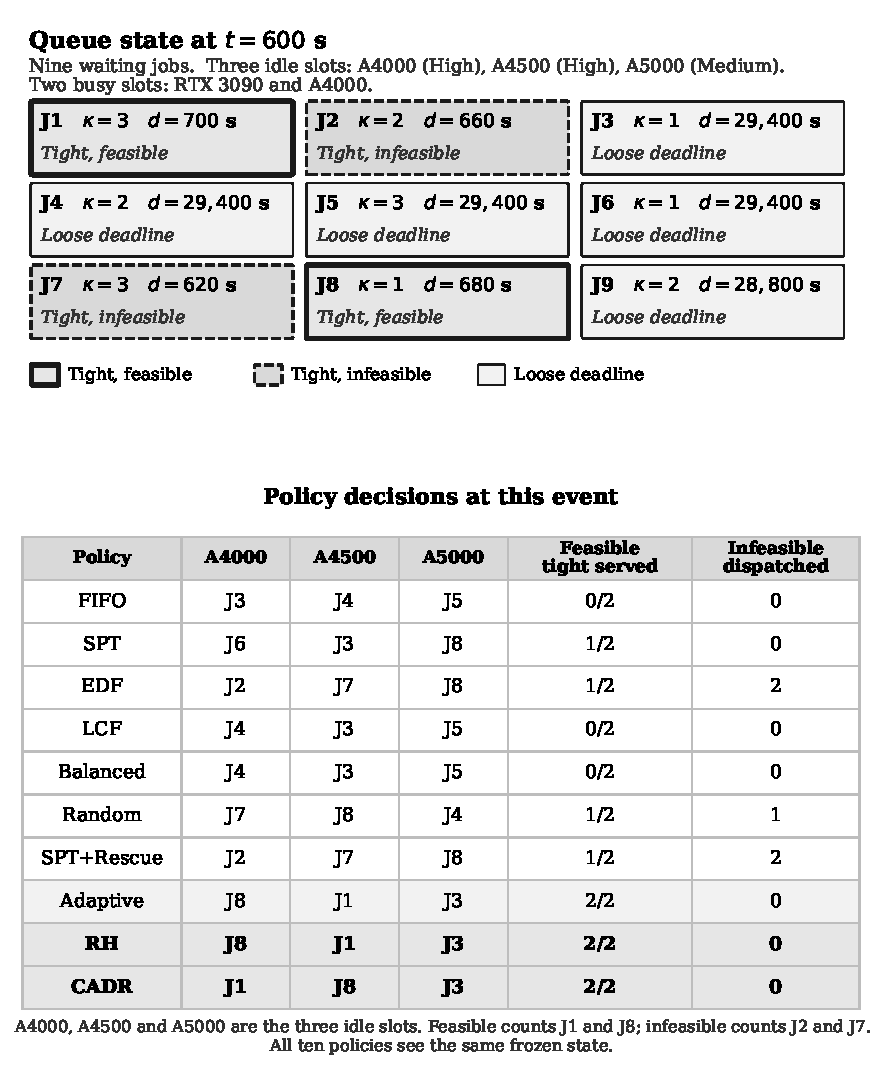
\includegraphics[width=\linewidth]{figures/snapshot_decision.pdf}
\caption[Frozen ten-policy decision snapshot]{Frozen ten-policy decision snapshot. The same queue and fleet state is presented to all ten schedulers at $t=600$\,s: nine waiting jobs, three idle slots (A4000, A4500, A5000) and two busy slots. Border weight and line style mark the tight jobs that can still meet their deadlines (J1, J8) and those that cannot under mean service times (J2, J7); the remaining jobs have loose deadlines. The table reports the job each policy assigns to each idle slot. This is an illustrative snapshot using the simulator's execution-time model and scheduler implementations, not a simulation run or a statistical result.}
\label{fig:snapshot-decision}
\end{figure}

\section{Metrics Collection}
\label{sec:metrics-collection}

The simulator records per-job metrics at the time of job completion:
\begin{itemize}
  \item $t_j^{\text{submit}}$, $t_j^{\text{start}}$, $t_j^{\text{complete}}$: timestamps in seconds
  \item $w_j = t_j^{\text{start}} - t_j^{\text{submit}}$: waiting time (Eq.~\ref{eq:wait})
  \item $r_j = t_j^{\text{complete}} - t_j^{\text{submit}}$: response time (Eq.~\ref{eq:resp}), tracked as a diagnostic; Chapter~\ref{chap:experiments} reports it through its two components rather than as a separate table column, since $r_j$ differs from the tabulated waiting time $w_j$ only by the realised execution time, whose per-policy differences enter through the cost metric
  \item $\delta_j = \mathbf{1}[t_j^{\text{complete}} \leq d_j]$: deadline adherence indicator (Eq.~\ref{eq:adherence}); the miss indicator is $1 - \delta_j$, and the miss rate is $\Delta_{\text{miss}} = \frac{1}{|\calJ|}\sum_{j}(1-\delta_j)$ (Eq.~\ref{eq:missrate})
  \item $c_j = W(\kappa_j, g_j) \cdot p_{g_j}$: job execution cost (Eq.~\ref{eq:cost_cost})
\end{itemize}

Fleet utilisation is recorded as an event-sampled series (one sample per processed event) together with a time series of idle and running slot counts; per-job provisioning delay is recoverable from each dispatch record as the gap between dispatch and execution start. All metrics are reported at the end of the simulation via \texttt{get\_\allowbreak metrics\_\allowbreak summary()}, which returns a structured dictionary used both for JSON export and for the PDF report generator.

Part of the verification half of the V\&V framework adopted in Chapter~\ref{chap:related} is executed rather than merely asserted. A constraint verifier re-checks completed runs on the seed-42 hectic-day workload against three model constraints: the seven baseline policies in the Phase~2 benchmark itself, and RH, CADR and the Adaptive hybrid in a companion run on the identical workload (\texttt{verify\_proposed.py}). Two of the checks are recomputed from the recorded per-job data rather than read from the accumulators that produced the summary: that every job's deadline-adherence flag agrees with its own recorded completion time and deadline, and that the reported miss count agrees with those flags; and that each job's cost equals $W(\kappa_j, g_j) \cdot p_{g_j}$. The third, that each job is dispatched once and each node holds at most one job at a time, is checked against a dispatch log that records every dispatch and is never overwritten. A job dispatched other than exactly once is a violation, as is any mismatch between the completion counter and the number of completed jobs, and no slot may hold two jobs whose occupancy intervals $[t_j^{\text{dispatch}}, t_j^{\text{complete}})$ overlap, provisioning wait included, which is Constraint~(\ref{eq:single_job_node}) itself; a job still held at the end of a run occupies its slot from dispatch onwards. All three checks report zero violations, over all 950 jobs, for all ten schedulers (in the \texttt{verification} block of the Phase~2 \texttt{report.json} and in \texttt{verification\_proposed.json}).

\chapter[Experimental Results and Analysis]{\texorpdfstring{Experimental Results\\and Analysis}{Experimental Results and Analysis}}
\label{chap:experiments}
{%

\section{Experimental Setup}
\label{sec:experimental-setup}

\subsection{Platform and Data}
\label{ssec:platform-and-data}

All experiments are conducted using the CGRSP simulator with per-stratum mean execution times derived from 6,234 real rendering jobs logged by the author's RunPod rendering pipeline between July 2025 and June 2026 (6,030 from its production Serverless endpoint, 203 tagged as development runs and one with no environment tag). Job timestamps are recorded in UTC by the originating AWS Lambda handler (verified against live CloudWatch logs) and are converted to Taiwan time (UTC+8) throughout this thesis for readability. The jobs span four GPU types (RTX~3090: 970 jobs, RTX~A5000: 4,680 jobs, RTX~A4000: 249 jobs, RTX~A4500: 335 jobs), three scene complexity levels, and a wide range of output resolutions (from small preview renders of a few thousand pixels to 48-megapixel stills). In the raw dataset, execution times range from 30 seconds to 352 seconds, with an aggregate coefficient of variation of $\approx$0.27 across the whole dataset and a smaller within-stratum dispersion (pooled $\sigma_{\ln} \approx 0.11$) once complexity and GPU type are fixed. Because the production logs record no scene metadata (polygon counts, materials), the complexity level of each job in the calibration dataset was assigned by render-time terciles of the empirical distribution; the simulator then treats $\kappa_j$ as an observable job attribute, corresponding to a deployment in which the studio classifies complexity from scene statistics known before rendering.

The realised execution time of job $j$ on GPU type $g$ is modelled as a log-normal random variable conditioned on the job's complexity level $\kappa_j \in \{1,2,3\}$ and the GPU type $g$:
\begin{equation}
W(j,g) \sim \text{LogNormal}\!\left(\mu_{\kappa_j,g},\, \sigma_{\kappa_j,g}^2\right),
\qquad
\mu_{\kappa,g} = \ln \overline{W}(\kappa,g) - \tfrac{1}{2}\sigma_{\kappa,g}^2,
\label{eq:lognormal}
\end{equation}
where $\overline{W}(\kappa,g)$ is the empirical mean execution time of the $(\kappa,g)$ stratum in the 6{,}234-job dataset (Table~\ref{tab:gpu_specs}; for a stratum with fewer than five observations it is an estimated mean, flagged in the table where the cell is shown). The location parameter $\mu_{\kappa,g}$ is centred so that $\mathbb{E}[W(j,g)] = \overline{W}(\kappa,g)$; consequently the mean execution times reported throughout this thesis and used in the numerical example (Section~\ref{sec:numerical-example}) are the expected values $\mathbb{E}[W(\kappa,g)]$. The log-normal form is appropriate because render times are strictly positive and right-skewed. The fit is moment-matched rather than tested with a formal goodness-of-fit statistic; the distributional robustness check used here is the mean-based rerun reported later in this section. The dispersion $\sigma_{\kappa,g}$ is fitted per stratum as the standard deviation of $\ln(\text{render time})$ within that stratum, ranging from $0.03$ for the most regular medium-complexity strata to $0.23$ for the most variable high-complexity stratum, with an n-weighted average of the per-stratum values of $\sigma_{\ln} \approx 0.11$ (a within-stratum coefficient of variation of about $0.11$; the variance-pooled standard deviation of the same strata would be about $0.13$); strata with fewer than five observations use that n-weighted average. (The larger aggregate coefficient of variation of $\approx 0.27$ measured across the whole dataset is dominated by between-complexity differences in the mean and is therefore not the relevant conditional dispersion.) The service time $W$ covers the render phase only (the \texttt{render\_time\_s} field of the dataset); the scene-import phase that preceded each render in production (mean 10.8\,s per job, about one seventh of the mean render time) is excluded from both slot occupancy and cost, so simulated per-job occupancy and cost are optimistic by roughly that proportion. The share varies by GPU type, from about 9\% of mean render time on the RTX~A4000 to about 16\% on the RTX~3090, so the size of the bias differs between schedulers that favour different GPU types; adding import time does not change the speed ordering of the four types. Schedulers plan with the deterministic estimate $\overline{W}(\kappa_j,g)$, that is, the expected service time $e_j$; only the realised completion time is stochastic, mirroring real operation where the dispatcher cannot observe a job's exact walltime in advance. Because render walltimes (tens to a few hundred seconds) are small relative to deadline windows ($T_{\text{tight}}$ to $T_{\text{loose}}$) and to queueing delays under saturation, this service-time stochasticity moves mean waits only modestly but matters more for miss rates: in a rerun of the 30 hectic seeds with the log-normal draw replaced by its stratum mean (\texttt{CGRSP/phase3\_diagnostics.py}), mean waits changed by at most \MeanSvcWaitMaxPct\% and miss rates by at most about \MeanSvcMissMaxRelPct\% in relative terms, both for the Adaptive hybrid; no other policy's miss rate moved by more than about 3\%. RH (\MeanSvcRHMiss\% miss) and CADR (\MeanSvcCADRMiss\%) keep their baseline order (paired $p=\MeanSvcRHvCADRp$), so the policy ranking does not hinge on the service noise, although the absolute miss levels in this chapter remain conditional on the log-normal service model. The effect can be slightly larger in lightly loaded, few-seed sub-experiments (for example, the surge-day deadline-tightness sweep), where outcomes near a crossover are more sensitive to the realised service times.

Operational costs are based on RunPod Secure Cloud prices from the 11~March 2026 pricing-API snapshot (Table~\ref{tab:gpu_specs}), treated as fixed deterministic constants throughout all simulations (RunPod prices change over time; these values represent a point-in-time snapshot): RTX~A5000 \$0.27/hr, RTX~3090 \$0.46/hr, RTX~A4500 \$0.25/hr, RTX~A4000 \$0.25/hr. At these Pods snapshot prices, the RTX~3090 is the most expensive GPU in the fleet at \$0.46/hr, approximately 70\% more expensive than the A5000, yet is no faster on the pooled average (72.9\,s vs 72.6\,s for A5000) and has the lower stratum mean only at low and high complexity; this price premium for almost no speed is the primary driver of the cost-aware scheduler designs (RH, CADR, Balanced). The A4500 and A4000 share the same hourly rate (\$0.25/hr) at this snapshot date, so cost differentiation between those two types is absent; the scheduler can exploit the speed difference between them without any cost penalty.

Figure~\ref{fig:data-overview} summarises the empirical dataset. The arrival pattern (panel~a) shows a pronounced peak between 14:00 and 17:00 Taiwan time, consistent with afternoon rendering bursts; the surge-day arrival rate (72 jobs/h) lies below the busiest recorded 60-minute window (119 jobs), whereas the hectic rate (360 jobs/h) is a stress-load assumption about 3.0 times that window. The execution-time distributions (panel~b) confirm right-skewed, GPU-dependent walltimes with medians ranging from 68\,s (RTX~A5000) to 87\,s (RTX~A4000), motivating the per-stratum log-normal service model.

\begin{figure}[H]
\centering
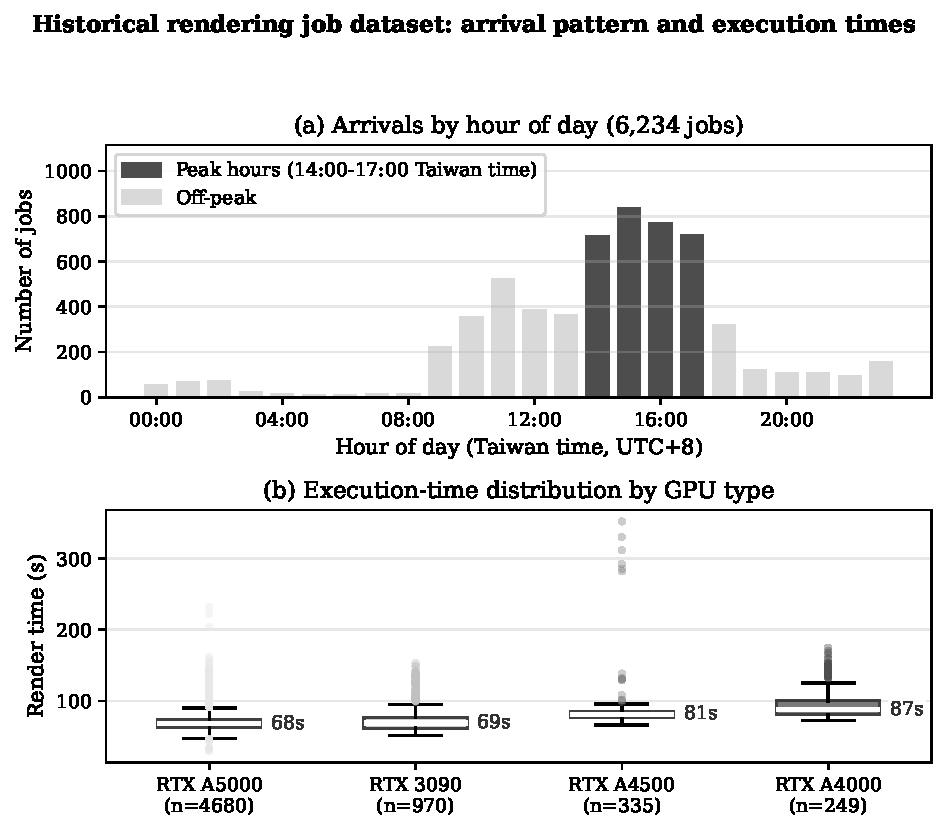
\includegraphics[width=0.97\textwidth]{figures/data_overview.pdf}
\caption[Empirical dataset: arrival pattern and execution times]{Empirical rendering job dataset (6,234 jobs, July 2025 to June 2026). (a)~Hourly arrival counts: the 14:00 to 17:00 Taiwan-time peak (dark grey), which the hectic and surge day types, as stress loads, exceed in daily volume (Section~\ref{ssec:platform-and-data}); off-peak hours are shown in light grey. (b)~Execution-time box plots per GPU type (IQR box, median white line, whiskers at 1.5$\times$IQR, outliers as dots): the RTX~A5000 is fastest (median 68\,s) and the RTX~A4000 slowest (median 87\,s), with right skew in all strata justifying the log-normal service model.}
\label{fig:data-overview}
\end{figure}

The simulation environment parameters are:
\begin{itemize}
  \item Simulation duration: 86,400 seconds (24 hours) per run
  \item Concurrency limit: $C_{\max} = 5$ (a baseline concurrency budget of five simultaneous GPU instances, equal to RunPod's default per-account worker quota~\cite{runpod2026maxworkers}; the quota rises with account balance, so $C_{\max}$ is swept in Table~\ref{tab:cmax_sensitivity})
  \item Job arrival: Poisson process with day-type-calibrated burst rate $\lambda$ and total job count $N_{\text{jobs}}$, a standard queueing-theory assumption representing independent submissions with memoryless inter-arrival times. These are independent parameters: the single-day experiments generate exactly $N_{\text{jobs}}$ candidate jobs with inter-arrival times $\sim\mathrm{Exp}(\lambda)$, so the active arrival window is approximately $N_{\text{jobs}}/\lambda$ seconds; the job count is $N_{\text{jobs}}$, not $\lambda \times 86{,}400$:
  \begin{itemize}[nosep, leftmargin=2em]
    \item Quiet: $\lambda=0.0008$ j/s, 6 jobs/day (arrival window $\approx$2.1\,hr)
    \item Normal: $\lambda=0.002$ j/s, $\sim$100 jobs/day (arrival window $\approx$13.9\,hr)
    \item Hectic: $\lambda=0.100$ j/s, $\sim$950 jobs/day (arrival window $\approx$2.6\,hr; capacity saturation $\rho>1$)
    \item Surge: $\lambda=0.020$ j/s, 730 jobs/day (arrival window $\approx$10.1\,hr)
  \end{itemize}
  The quiet count is of the order observed in the job record. The normal count (100) is above a typical recorded day: the normal-class billing days imply about 27 jobs at RunPod's Serverless Flex rates, and recorded days of 10 to 79 jobs average about 32 (the largest holds 78), so a simulated normal day is moderately loaded rather than typical. The hectic and surge counts are stress-load modelling assumptions rather than counts observed in the job record: the surge count matches the average spend of the surge-class billing days at the same rates (about 750 jobs), but the hectic count is a saturating burst of the order of the single busiest billing day (about 1,070 jobs), roughly ten times what the average hectic-class billing day implies (about 90 jobs); the busiest day in the 6,234-job record holds 415 jobs (18~September 2025, Taiwan time).
  \item Deadline: heterogeneous distribution: 20\% of jobs have a tight 1-hour deadline ($T_{\text{tight}}=3{,}600$\,s, rush orders) and 80\% have a loose 8-hour deadline ($T_{\text{loose}}=28{,}800$\,s, standard renders). Objective weights: $\alpha_1 = 1$ (penalty per second of wait) and $\alpha_2 = 10$ (penalty per missed deadline); the ratio $\alpha_2/\alpha_1 = 10$ is swept in Section~\ref{ssec:objective-weight-sensitivity}. This split is a modelling assumption reflecting a rendering studio context in which a minority of frames are time-critical (client delivery, real-time preview) while the majority are standard batch renders with flexible delivery windows. A uniform deadline distribution would fail to reveal the starvation-deadline trade-off between SPT and SPT+Rescue. The sensitivity of all results to this assumption is assessed explicitly in Section~\ref{ssec:deadline-tightness-sensitivity}, which sweeps the tight-deadline fraction from 10\% to 90\%.
  \item Availability: each rental request incurs a stock-status-dependent provisioning delay $\tau^{\text{prov}}_j$ (formalised in Section~\ref{sec:mathematical-model}, Eq.~\ref{eq:provdelay}). The model treats the platform as an on-demand Secure Cloud pool in which every slot is rentable at any time and a running instance is never reclaimed by the provider, so market scarcity is represented not as denial of service but purely as this provisioning delay. The availability model is informed by RunPod pricing-API snapshots collected between 11~March and 20~April 2026 (5,294 raw snapshots; 77 per-run distribution summaries (usually two runs per collection day) spanning that same 11~March to 20~April collection window were used during calibration): the snapshots supply the secure-cloud hourly prices, the qualitative stock-status vocabulary (High/Medium/Low), and the diurnal demand shape. Snapshot timestamps are tagged UTC by the scraper's own code, but the scraping machine's system clock was in fact running on GMT+7; snapshot hours are therefore shifted by $+1$\,h to Taiwan time (UTC+8) throughout this thesis, consistent with the job-arrival timestamps (which are genuine UTC, shifted by $+8$\,h). The per-type baseline high-stock probabilities $\beta_g$ (RTX~3090 50\%, RTX~A5000 65\%, RTX~A4500 70\%, RTX~A4000 75\%) are \emph{modelling assumptions} for the on-demand secure pool rather than empirical frequencies from the snapshot record: the stock-status field returned by the pricing API (queried for a single-GPU Secure Cloud offer) reports the four fleet types as almost never High and, in a substantial share of snapshots, with no Secure Cloud offer at all (Figure~\ref{fig:availability-history}); read literally this would imply intermittent denial of service, which the model deliberately excludes, so $\beta_g$ encodes an assumed probability that an on-demand request is fulfilled promptly rather than a frequency read from that field. The time-of-day multiplier $\phi(t)$ scales the high-stock probability and is expressed on the simulator's own local clock, which is Taiwan time throughout this project: off-peak, 00:00 to 06:00 ($\times$1.3); morning, 06:00 to 12:00 ($\times$0.9); peak, 12:00 to 18:00 ($\times$0.5); evening, 18:00 to 24:00 ($\times$1.0); the observed record supports this shape qualitatively, with Secure Cloud availability of the fleet types visibly worse during the business-hours peak (Figure~\ref{fig:availability-history}b). Simulation time zero is anchored to 08:00 on the modelled day, matching a studio working day that opens in the morning rather than at midnight, so every run starts in the morning band; the offset is applied arithmetically rather than read from the host machine's clock, so the sequence of bands a run traverses does not depend on the timezone it happens to execute under. Outside the peak band the multiplier keeps $p^{H}_g + p^{M}_g \ge 1$ for all four fleet types, so the Low state is then unreachable; only during the peak band (multiplier $\times 0.5$) does it become reachable at all, and there for all four types, with per-draw probability largest for the low-$\beta_g$ types (37.5\% for the RTX~3090 down to 6.25\% for the RTX~A4000). Because the peak occupies a minority of the day, the time-weighted Low probability is modest, but it is not negligible: instrumenting the delay draw over ten seeds of the FIFO, SPT and EDF runs in the Phase~3 day-type sensitivity runs gives Low-range delays (600\,s or more) on about 3\% of dispatches on hectic and surge days, about 7 to 11\% on normal days (where the few jobs arrive spread across the day, so a larger share meet the peak band), and none on quiet days; on the Phase~4 monthly calendar the shares are about 5 to 8\% on normal days and small but non-zero (about 0.3 to 1.1\%) on quiet days; all other delays are in the High and Medium ranges (at most two minutes). Provisioning delays are drawn uniformly from stock-status ranges: High 0 to 10\,s, Medium 30 to 120\,s, Low 600 to 7200\,s. (Implementation note: the status a scheduler observes is the draw made at the most recent earlier dispatch, and every type reads High before a run's first dispatch. The status realised at acquisition is a fresh, independent draw from the same time-varying model. The observation therefore behaves like a stale marketplace poll rather than a binding quote: apart from what the type's $\beta_g$ and the time-of-day band already imply, it carries no information about the delay the dispatched job then pays. The same observation mechanism applies to every scheduler.) Figure~\ref{fig:diurnal-model} shows the $\phi(t)$ step function alongside the real job arrival pattern; the 77 calibration snapshots are concentrated at hours 02:00 to 03:00 and 19:00 to 20:00 Taiwan time, so $\phi(t)$ is a parametric calibration rather than a pointwise empirical fit.
\end{itemize}

\begin{landscape}
\begin{figure}[H]
\centering
\captionsetup{font=small,skip=6pt}
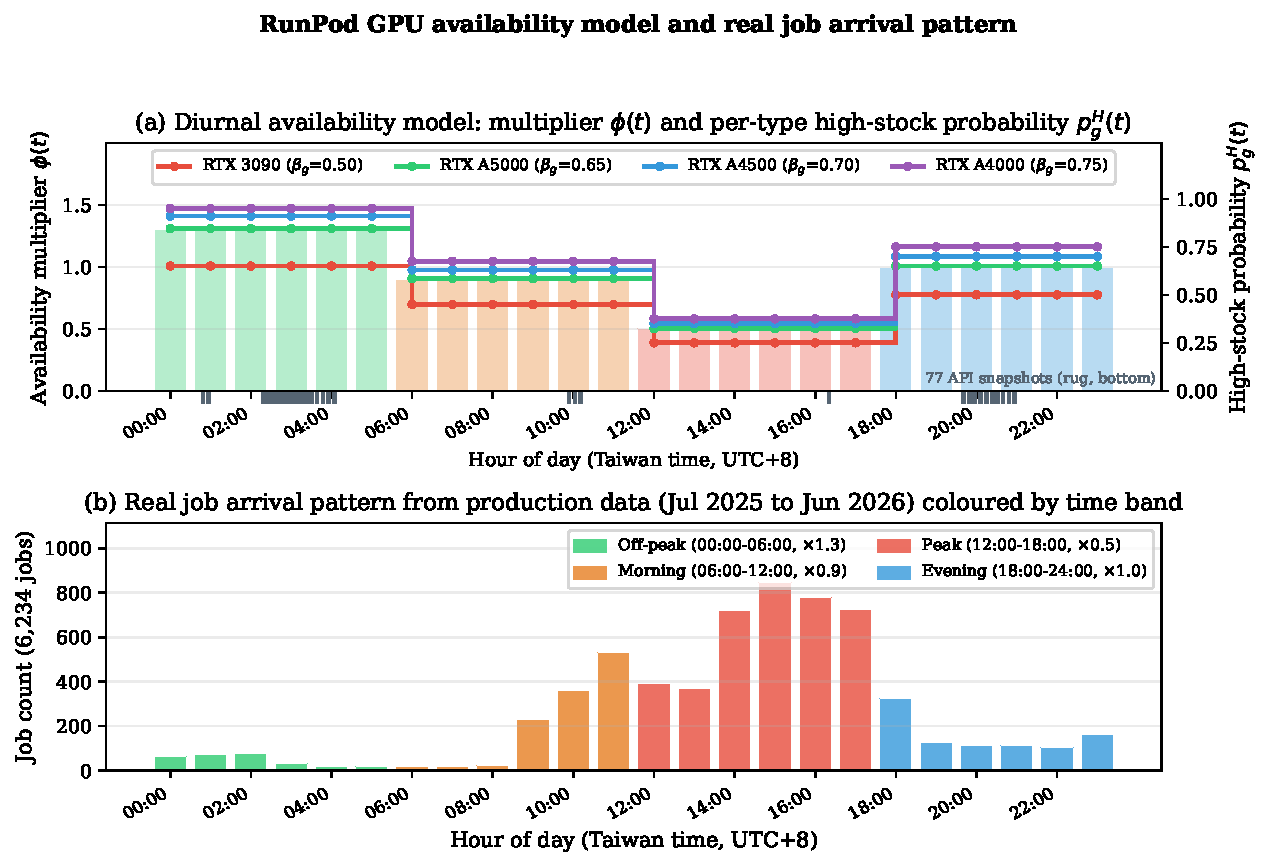
\includegraphics[width=0.98\linewidth,height=0.90\textheight,keepaspectratio]{figures/diurnal_model.pdf}
\caption[Diurnal availability model and real arrival pattern]{Diurnal availability model and real arrival pattern.}
\label{fig:diurnal-model}
\end{figure}
\end{landscape}

\noindent\textit{Figure~\ref{fig:diurnal-model} notes.} Diurnal availability model and real job arrival pattern, all times Taiwan time (UTC+8), matching the simulator's own local clock (Section~\ref{sec:mathematical-model}). (a)~Bars (left axis) show the parametric step function $\phi(t)$: off-peak 00:00 to 06:00 raises availability ($\times$1.3, green); morning 06:00 to 12:00 moderately reduces it ($\times$0.9, orange); peak 12:00 to 18:00 reduces availability by half ($\times$0.5, red); evening 18:00 to 24:00 is neutral ($\times$1.0, blue). Lines (right axis) show the resulting per-type high-stock probability $p_g^H(t) = \min(0.95,\,\beta_g\,\phi(t))$ for each of the four fleet GPUs, using each type's baseline $\beta_g$ (RTX~3090 50\%, RTX~A5000 65\%, RTX~A4500 70\%, RTX~A4000 75\%): the four curves share $\phi(t)$'s step shape but sit at different levels set by $\beta_g$, and the RTX~A4000 curve flattens against the 0.95 ceiling during the off-peak band ($0.75 \times 1.3 = 0.975 \to 0.95$). Rug marks at the bottom show the 77 RunPod API snapshot times, which are concentrated in two narrow windows. (b)~Actual hourly job count from the 6,234 logged rendering jobs (July 2025 to June 2026; 6,030 production, 203 development, one untagged), coloured by the corresponding $\phi(t)$ band. The historical arrival peak at 14:00 to 17:00 Taiwan time falls inside the peak band, so the busiest hours of the production record coincide with the model's lowest-availability window. The simulated day is anchored differently: simulation time zero corresponds to 08:00 Taiwan time (Section~\ref{ssec:platform-and-data}), so a run opens in the morning band ($\times$0.9), and the hectic day's arrival window of roughly 2.6~hours lies wholly inside it; only the longer surge and normal arrival windows extend into the afternoon peak at all. Panel~(b) therefore describes when the studio historically submitted work; in the simulated hectic day the arrivals fall in the morning band, while the saturated backlog they create is still being dispatched through the afternoon peak band, where stock status and provisioning delay are drawn at dispatch time.\par

\begin{landscape}
\begin{figure}[H]
\centering
\captionsetup{font=small,skip=6pt}
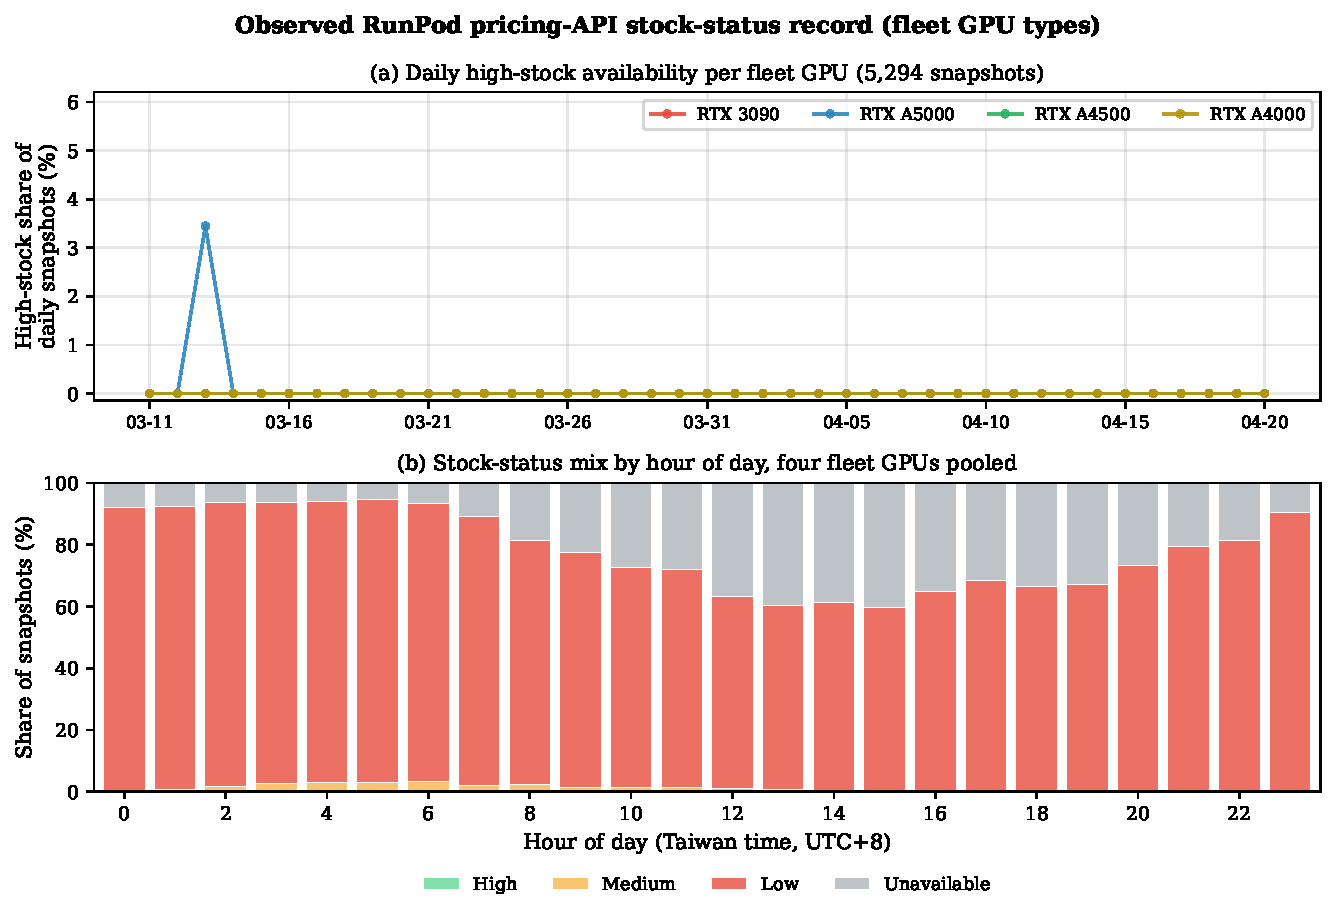
\includegraphics[width=0.98\linewidth,height=0.85\textheight,keepaspectratio]{figures/availability_history.pdf}
\caption[Observed RunPod availability record]{Observed RunPod availability record.}
\label{fig:availability-history}
\end{figure}
\end{landscape}

\noindent\textit{Figure~\ref{fig:availability-history} notes.} Observed RunPod availability record for the four fleet GPU types, 11~March to 20~April 2026 (5,294 pricing-API snapshots). (a)~Daily share of snapshots reporting High stock: essentially zero throughout the collection window. (b)~Stock-status mix by hour of day (fleet types pooled): the Secure Cloud single-GPU listing for these consumer-tier types is chronically Low-stock, and the share of snapshots with no Secure Cloud offer (Unavailable) rises during the business-hours window, qualitatively consistent with the peak-demand reduction encoded in $\phi(t)$. Because the model excludes the no-offer state this record shows, the baseline high-stock probabilities $\beta_g$ are treated as modelling assumptions for the on-demand pool; the snapshot record contributes the fleet prices, the stock-status vocabulary, and the diurnal demand shape.\par

\subsection{Evaluation Phases}
\label{ssec:evaluation-phases}

Four phases of evaluation are conducted (phases are numbered from 2; Phase~1 comprised initial exploratory calibration runs not reported here):

\begin{description}
  \item[Phase 2] Single-seed benchmark (seed=42) on the hectic-day configuration of Section~\ref{ssec:platform-and-data}. Provides illustrative point estimates for the seven baseline schedulers (all but RH, CADR and the Adaptive hybrid) under capacity saturation ($\rho>1$; RH, CADR, and the Adaptive hybrid enter at Phase~3); being single-seed it carries no confidence interval and is superseded by the $n=30$ Phase~3 statistics for every inferential claim.
  \item[Phase 3 Statistical] 30 independent replications (seeds 0 to 29) on hectic-day workload ($\sim$950 jobs/day). Computes 95\% confidence intervals and paired $t$-tests (with a Wilcoxon signed-rank backup) and Cohen's $d$ for pairwise comparisons. Includes RH, CADR, and the CADR-order-only (CADR-OO) ablation variant. Tardiness (mean minutes past deadline) is reported as a diagnostic alongside miss rate.
  \item[Phase 3 Sensitivity] Compares all schedulers across four operationally calibrated day types (quiet/normal/hectic/surge) at $C_{\max}=5$, with 30 seeds per day type (1{,}200 total runs). Identifies the load regime where scheduler differences become operationally significant.
  \item[Phase 4] 30-day monthly simulation (10~replications; the type of each day, one of quiet, normal, hectic and surge, is drawn from day-of-week probabilities estimated by classifying the 30 complete days of RunPod billing between 22~April and 21~May 2026 by daily spend). Aggregates scheduler performance across monthly workload variation to assess behaviour over a mixed month. Each replication uses one persistent fleet and queue for all 30 days. Daily Poisson traces are capped at the sampled candidate job count and cut off at the next day boundary; jobs already accepted continue across boundaries, and after the final boundary the simulator drains the remaining backlog. Metrics are grouped by submission day and use accepted jobs as the denominator. Ten replications rather than 30 were used because each replication simulates a complete calendar; 10 replications yield 95\% CIs with $t^*_9 = 2.262$, providing adequate precision for the monthly comparison objective.
\end{description}

A \textbf{deadline tightness sensitivity} study sweeps tight-deadline fraction $f_{\text{tight}} \in \{10\%,\allowbreak 30\%,\allowbreak 50\%,\allowbreak 70\%,\allowbreak 90\%\}$ under surge-day conditions ($C_{\max}=5$, $\lambda=0.020$ j/s, 730 jobs/day, 30 seeds each) to identify the load regime where EDF's deadline-safety advantage over SPT is maximised.

\subsection{Statistical Methodology}
\label{ssec:statistical-methodology}

All statistical comparisons use a paired $t$-test on the per-seed averages, with a Wilcoxon signed-rank test~\cite{wilcoxon1945individual} as a distribution-free backup. Every scheduler is evaluated on the same 30 seeds with identical generated jobs per seed, so the per-seed observations are matched (a randomised block design); the paired test is therefore both valid and more powerful than an unpaired alternative, as it removes the between-seed variance that the schedulers share. Effect sizes are reported as Cohen's $d = (\mu_1 - \mu_2) / s_{\text{pooled}}$, where $s_{\text{pooled}}$ is the pooled standard deviation. The threshold $|d| \geq 0.8$ is used as the criterion for a practically meaningful effect (``large'' by Cohen's convention~\cite{cohen1988statistical}). Confidence intervals are computed as $\bar{x} \pm t^*_{n-1} \cdot (s/\sqrt{n})$ with $t^*_{29} = 2.045$ for $n=30$, $\alpha=0.05$. For each pairwise comparison it prints, Table~\ref{tab:ttests} also reports the paired mean difference with its 95\% confidence interval, $\bar{d} \pm t^*_{29}\, s_d/\sqrt{n}$, so that each printed effect is stated with its uncertainty~\cite{kalibera2020quantifying,krishnamachari2026statistical}. The $t$-based intervals and tests rely on the per-seed means being approximately normally distributed, which the central limit theorem supports for averages over independent replications~\cite{law2000simulation}; because the number of replications this requires depends on how skewed the underlying metric is, the Wilcoxon signed-rank test above serves as the distribution-free check. Consistent with the lexicographic objective (Eq.~\ref{eq:objective}), which prioritises QoS over operational cost rather than collapsing them into one scalar, all experimental comparisons report each component separately (average waiting time, deadline miss rate, operational cost) rather than as an aggregate. Decomposed reporting enables direct identification of which dimension drives scheduler differences: a scheduler that reduces miss rate by increasing waiting time would appear identically weighted in a scalar objective but the trade-off is transparent in the decomposed view. Each pairwise comparison in Table~\ref{tab:ttests} tests a pre-specified directional hypothesis grounded in scheduling theory (e.g.\ SPT reduces wait by shortest-job-first ordering; EDF reduces miss by deadline ordering) rather than a data-driven hypothesis selection; a Holm-Bonferroni step-down correction~\cite{holm1979simple} over the full pairwise family is nonetheless applied to control the family-wise error rate; as reported below, most but not all comparisons significant at the uncorrected level survive it.

\section{Phase 2: Seven-Scheduler Benchmark}
\label{sec:phase-2-seven-scheduler-benchmark}

Table~\ref{tab:phase2} and Figure~\ref{fig:phase2} report Phase~2 results for all seven schedulers on a hectic day; Figure~\ref{fig:phase2} additionally contrasts a normal day (top row), where all schedulers achieve near-zero miss, to show that the saturated hectic day is the regime in which scheduler choice matters.

\begin{table}[htbp]
\centering
\caption[Phase 2 benchmark results]{Phase 2 benchmark: hectic day ($\sim$950 jobs/day), $C_{\max}=5$, seed=42, $\lambda=0.100$ j/s, 20\% tight 1h / 80\% loose 8h deadlines (capacity saturation: $\rho>1$). Util is event-sampled (mean of per-event fleet-occupancy samples over the active window), not a time-weighted day average.}
\label{tab:phase2}
\begin{tabular}{lrrrrr}
\toprule
\textbf{Scheduler} & \textbf{Avg Wait (min)} & \textbf{Miss \%} & \textbf{Cost (\$)} & \textbf{Util (\%)} & \textbf{Completed} \\
\midrule
\textbf{SPT+Rescue} & 144.02 & \textbf{9.37} & 6.28 & 95.7 & 950/950\\
\textbf{SPT} & \textbf{140.02} & 19.16 & 6.25 & 95.7 & 950/950\\
EDF & 174.21 & 12.11 & 6.30 & 95.7 & 950/950\\
LCF & 157.06 & 16.95 & 6.24 & 95.7 & 950/950\\
Balanced & 174.09 & 24.53 & 6.33 & 95.7 & 950/950\\
FIFO & 165.26 & 23.37 & 6.40 & 95.7 & 950/950\\
Random & 174.35 & 25.26 & 6.34 & 95.7 & 950/950\\
\bottomrule
\end{tabular}

\end{table}

\begin{landscape}
\begin{figure}[H]
\centering
\captionsetup{font=small,skip=6pt}
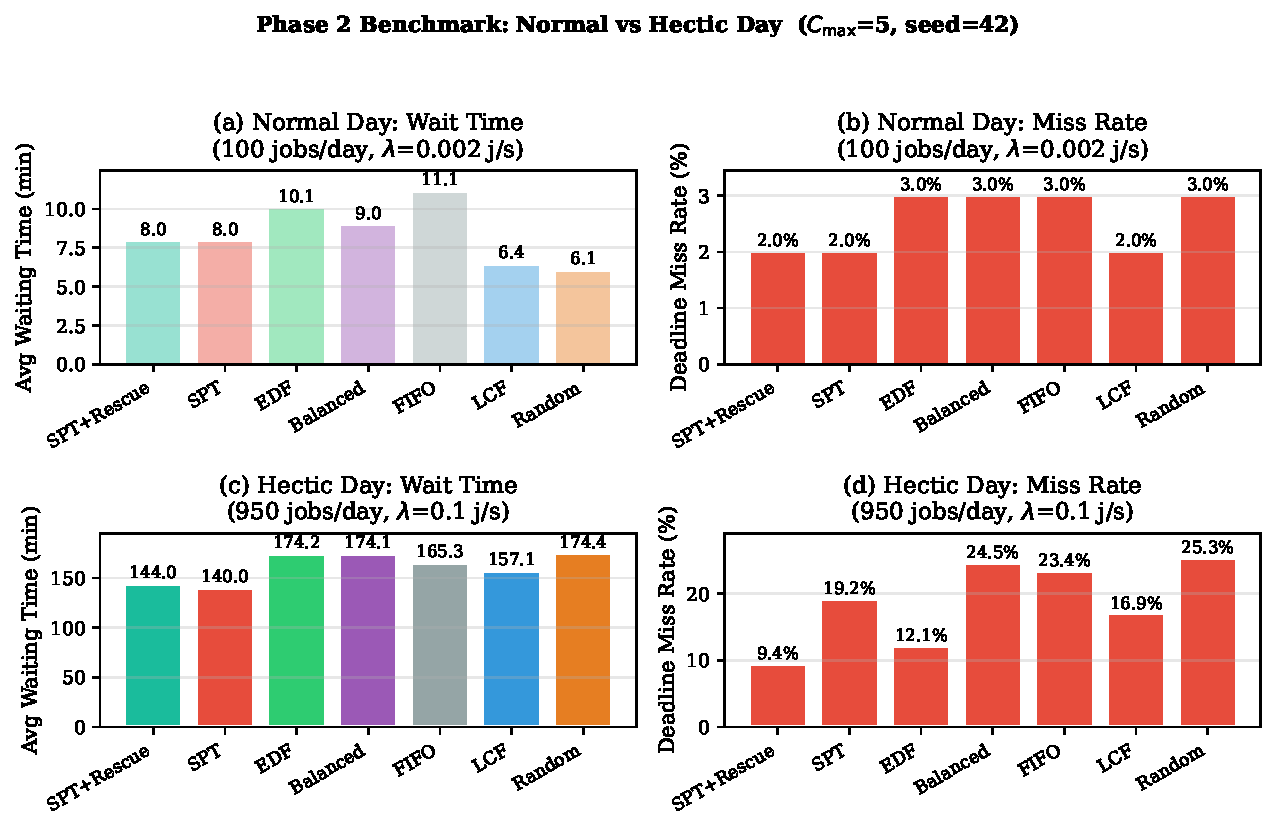
\includegraphics[width=0.98\linewidth,height=0.80\textheight,keepaspectratio]{figures/phase2_comparison.pdf}
\caption[Phase 2 benchmark: normal vs hectic day]{Phase 2 benchmark: normal vs hectic day.}
\label{fig:phase2}
\end{figure}
\end{landscape}

\noindent\textit{Figure~\ref{fig:phase2} notes.} Phase 2 benchmark results ($C_{\max}=5$, seed=42, 20\% tight 1h / 80\% loose 8h deadlines). Top row: a normal day ($\sim$100 jobs/day, $\rho<1$), where all schedulers achieve near-zero miss and wait under about 12~minutes, confirming that scheduler choice is immaterial under light load. Bottom row: the hectic day ($\sim$950 jobs/day, $\lambda=0.100$ j/s; capacity saturation), the discriminating regime analysed below. In this seed SPT+Rescue records the lowest miss (\PhTwoRescueMiss\%, at \PhTwoRescueWait~min wait) and SPT the lowest wait (\PhTwoSPTwait~min) of the seven baseline schedulers; SPT's miss (\PhTwoSPTmiss\%) is about twice SPT+Rescue's; EDF's miss (\PhTwoEDFmiss\%) is lower here than its 30-seed Phase~3 mean, illustrating single-seed variance under saturation; FIFO, LCF, and Balanced ignore deadlines, and FIFO's miss (\PhTwoFIFOmiss\%) is high but not the highest of the seven in this seed (Balanced and Random are higher).\par

Four observations follow from Phase~2, though as a single seed it carries no confidence interval and several of the following patterns do not survive to the robust $n=30$ Phase~3 mean; that comparison is made explicit below. First, in this seed SPT has the lowest waiting time (\PhTwoSPTwait~min) and SPT+Rescue the lowest miss rate (\PhTwoRescueMiss\%) of the seven baseline schedulers, with SPT+Rescue's wait four minutes higher (\PhTwoRescueWait~min): the laxity rescue mechanism trades a little wait for a large miss reduction on this particular seed, the same direction as the $n=30$ result (Section~\ref{sec:phase-3-statistical-validation}), where SPT and RH have no significant paired wait difference and form the lowest-wait tier and SPT+Rescue trails both; the single seed nevertheless shows a larger gap than the mean, which is why Phase~3's 30-seed replication, not this single seed, is the basis for every inferential claim in this thesis. Second, SPT's miss rate in this seed (\PhTwoSPTmiss\%) is about twice that of SPT+Rescue, a larger ratio than at $n=30$, consistent with shortest-job-first ordering sacrificing tight-deadline jobs under saturation. Third, EDF's miss rate in this seed (\PhTwoEDFmiss\%) is lower than its Phase~3 mean of \EDFmiss\% ($n=30$), reflecting high seed-to-seed variance under saturation, so the Phase~3 result provides the reliable cross-seed estimate rather than this seed's draw. Fourth, FIFO processes jobs without deadline awareness and has a high miss rate (\PhTwoFIFOmiss\%), though in this seed Balanced and Random are worse on miss: under saturation, a large fraction of tight-deadline jobs fail to complete within 1 hour. Across all policies, the schedulers achieve \PhTwoUtilPct\% event-sampled concurrency utilisation and 100\% job completion (all 950 jobs dispatched); the utilisation figure is the mean of per-event samples, which concentrate on the busy active window, and is not a time-weighted average over the full 24-hour day, most of which lies after the backlog drains.

\section{Phase 3 Statistical Validation}
\label{sec:phase-3-statistical-validation}

Table~\ref{tab:statistical} reports Phase~3 results over $n=30$ seeds on hectic-day workload (configuration in Section~\ref{ssec:platform-and-data}), with 95\% confidence intervals. Figure~\ref{fig:phase3-ci} plots the same intervals graphically, showing each scheduler's own across-seed spread; because the schedulers share seeds, overlap of these marginal intervals is not a test of any pair, and the paired mean differences and tests in Table~\ref{tab:ttests} give the verdict for the pairs compared there.

\begin{table}[htbp]
\centering
\caption[Phase 3 statistical validation]{Phase 3 statistical validation: $n=30$ seeds, hectic day ($C_{\max}=5$, $\sim$950 jobs/day, $\lambda=0.100$ j/s, 20\% tight 1h / 80\% loose 8h deadlines; capacity saturation $\rho>1$)}
\label{tab:statistical}
\resizebox{\linewidth}{!}{\begin{tabular}{lrrrrrr}
\toprule
\textbf{Scheduler} & \textbf{Avg Wait (min)} & \textbf{95\% CI} & \textbf{Miss \%} & \textbf{95\% CI} & \textbf{Avg Tardiness (min)} & \textbf{Cost (\$)} \\
\midrule
\textbf{RH} & 141.70 & [137.90,~145.50] & \textbf{9.60} & [8.41,~10.78] & 31.84 & 6.35\\
CADR & 144.66 & [141.35,~147.97] & 9.68 & [8.18,~11.18] & 5.95 & 6.36\\
SPT+Rescue & 146.32 & [143.28,~149.36] & 13.56 & [12.45,~14.68] & 5.89 & 6.37\\
Adaptive & 169.67 & [165.97,~173.36] & 12.62 & [11.08,~14.16] & 4.91 & 6.39\\
\textbf{SPT} & \textbf{141.45} & [137.52,~145.38] & 18.96 & [17.26,~20.67] & 12.02 & 6.34\\
EDF & 170.22 & [166.99,~173.45] & 14.71 & [13.28,~16.13] & 5.16 & 6.41\\
LCF & 166.91 & [164.03,~169.79] & 24.24 & [22.97,~25.51] & 25.25 & 6.37\\
Balanced & 168.59 & [165.50,~171.69] & 25.25 & [24.18,~26.31] & 26.66 & 6.38\\
FIFO & 167.93 & [164.10,~171.75] & 24.43 & [23.14,~25.72] & 26.01 & 6.40\\
Random & 167.68 & [164.62,~170.74] & 23.44 & [22.64,~24.24] & 32.89 & 6.38\\
\bottomrule
\end{tabular}
}
\end{table}

\begin{figure}[htbp]
\centering
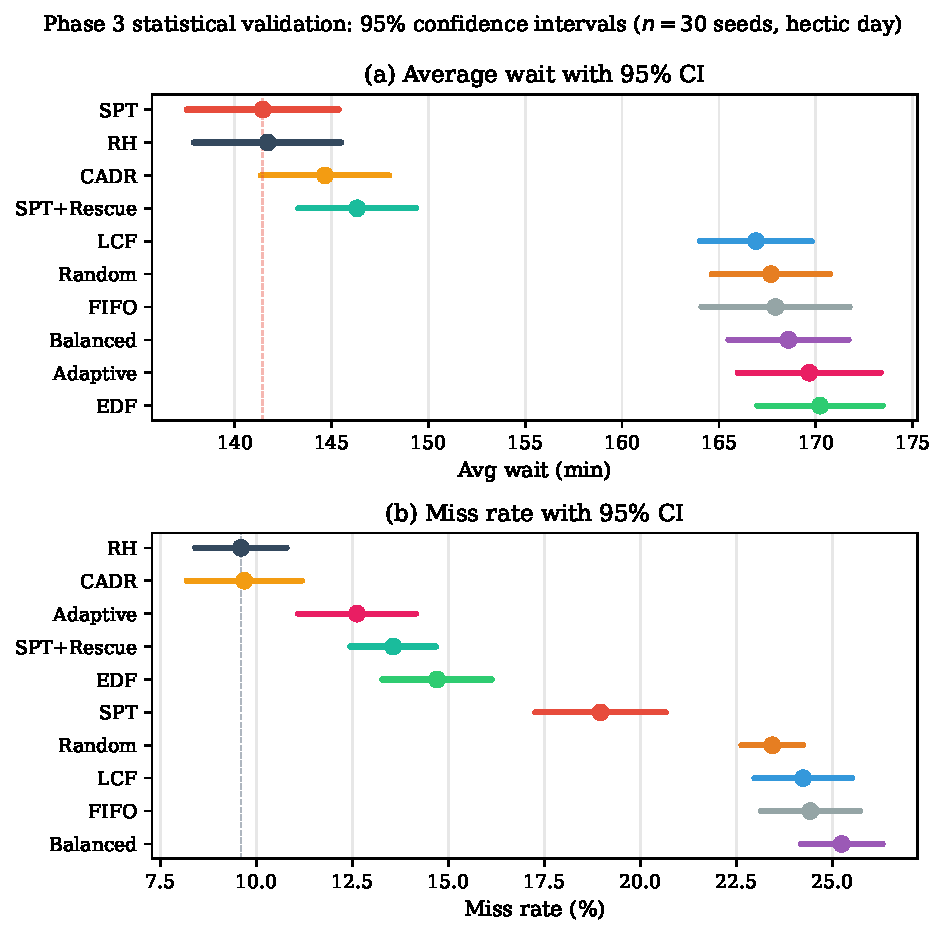
\includegraphics[width=0.97\textwidth]{figures/phase3_ci.pdf}
\caption[Phase 3: 95\% confidence intervals]{Phase 3 confidence interval plot: 95\% CIs for average wait (a) and miss rate (b) for all ten schedulers, $n=30$ seeds, hectic day. Schedulers are ordered by mean value within each panel. These are marginal intervals summarising each scheduler's own across-seed variability, so they describe the spread of the ten distributions and are not themselves a test of any pair. Because every scheduler is run on the same 30 seeds (a randomised block design, Section~\ref{ssec:statistical-methodology}), the paired tests of Table~\ref{tab:ttests} are the authoritative verdict, and overlap here need not agree with them in either direction: EDF's and FIFO's wait intervals overlap although that pair separates at the uncorrected level, and EDF's and SPT's miss intervals overlap by a hair although the paired test separates them clearly ($p<0.001$). Key groupings: RH and CADR have the lowest miss point estimates, with no significant paired difference (paired $t=\RHCADRmissT$, $p=\RHCADRmissP$; this does not establish equivalence); SPT and RH are tied for the lowest wait (paired $t=\RHSPTwaitT$, $p=\RHSPTwaitP$); EDF achieves significantly lower miss than SPT despite much higher wait, underscoring that deadline-awareness and throughput are separate design levers.}
\label{fig:phase3-ci}
\end{figure}

\begin{figure}[H]
\centering
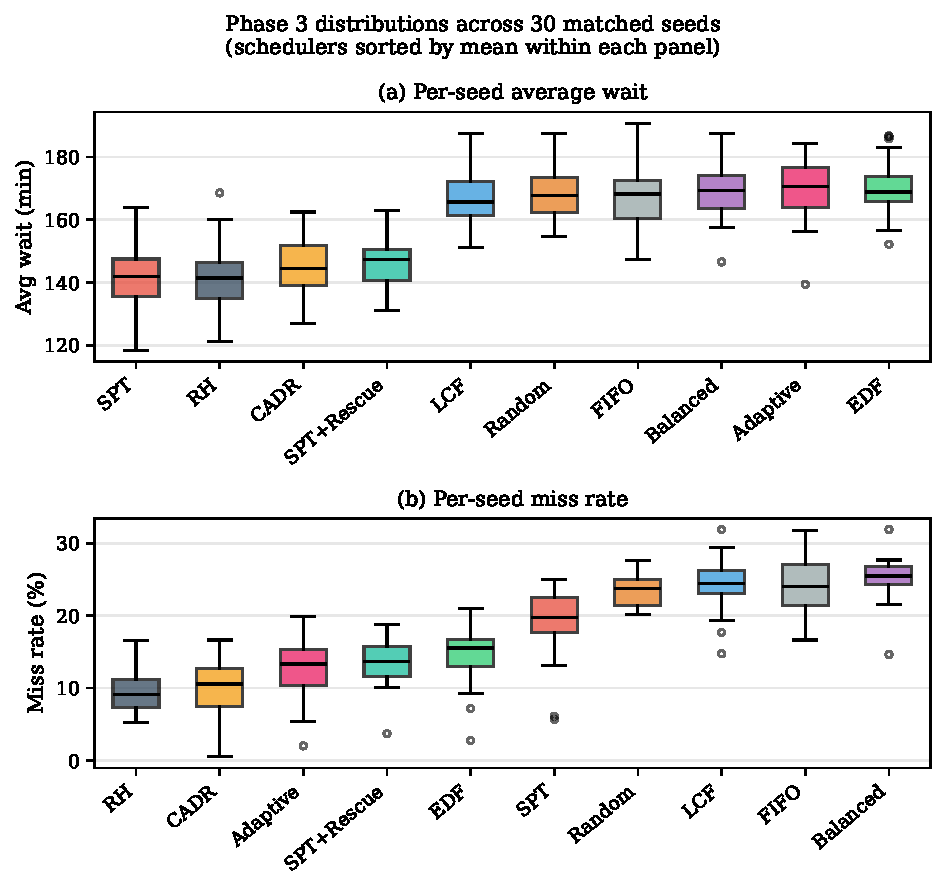
\includegraphics[width=0.97\textwidth]{figures/seed_distributions.pdf}
\caption[Phase 3: per-seed distributions]{Per-seed distributions behind the Phase 3 means: box plots of average wait (a) and miss rate (b) across the 30 matched seeds, schedulers sorted by mean within each panel. The box spans the interquartile range with the median line; whiskers extend to 1.5$\times$IQR and dots mark outlier seeds. The clear vertical separation between the deadline-aware and deadline-oblivious groups in panel~(b) holds seed by seed, not just on average, which is what the paired tests in Table~\ref{tab:ttests} formalise.}
\label{fig:seed-distributions}
\end{figure}

Figure~\ref{fig:seed-distributions} complements the interval view with the full per-seed distributions, showing that the group separations hold across individual seeds rather than only in the aggregate. Table~\ref{tab:ttests} reports the pairwise paired $t$-test results.

\begin{table}[htbp]
\centering
\caption[Pairwise paired t-test results]{Pairwise paired $t$-test results, Phase 3 ($n=30$, $C_{\max}=5$, hectic day $\sim$950 jobs/day, 20\% tight 1h / 80\% loose 8h deadlines). Each comparison is matched on seed; a Wilcoxon signed-rank test gives raw $p<0.05$ for every entry marked significant. ``Significant?'' reflects the Holm-Bonferroni-corrected verdict at family-wise $\alpha=0.05$ (Section~\ref{ssec:statistical-methodology}), not the raw uncorrected $p$-value; $^\dagger$marks the two comparisons whose raw $p<0.05$ but which do not survive the correction. Mean differences are first-named minus second-named scheduler (minutes for wait, percentage points for miss), with a paired $t$-based 95\% confidence interval ($\mathrm{df}=29$) that is unadjusted for multiplicity, so the two $^\dagger$ rows exclude zero at the raw level while failing the Holm-corrected test.}
\label{tab:ttests}
\small
\resizebox{\textwidth}{!}{%
\begin{tabular}{llrrlrr}
\toprule
\textbf{Comparison} & \textbf{Metric} & $t$ & $p$-value & \textbf{Significant?} & Mean diff.\ [95\% CI] & Cohen's $d$ \\
\midrule
SPT vs FIFO        & Avg wait   & $\SPTFIFOwaitT$    & $<0.001$           & Yes & $\SPTFIFOwaitMD$ [$\SPTFIFOwaitMDLo$, $\SPTFIFOwaitMDHi$] & $\SPTFIFOwaitD$ \\
SPT vs FIFO        & Miss rate  & $\SPTFIFOmissT$    & $<0.001$           & Yes & $\SPTFIFOmissMD$ [$\SPTFIFOmissMDLo$, $\SPTFIFOmissMDHi$] & $\SPTFIFOmissD$ \\
SPT+Rescue vs FIFO & Avg wait   & $\RescueFIFOwaitT$ & $<0.001$           & Yes & $\RescueFIFOwaitMD$ [$\RescueFIFOwaitMDLo$, $\RescueFIFOwaitMDHi$] & $\RescueFIFOwaitD$ \\
SPT+Rescue vs FIFO & Miss rate  & $\RescueFIFOmissT$ & $<0.001$           & Yes & $\RescueFIFOmissMD$ [$\RescueFIFOmissMDLo$, $\RescueFIFOmissMDHi$] & $\RescueFIFOmissD$ \\
EDF vs FIFO        & Avg wait   & $\EDFFIFOwaitT$    & $\EDFFIFOwaitP$    & No  & $\EDFFIFOwaitMD$ [$\EDFFIFOwaitMDLo$, $\EDFFIFOwaitMDHi$] & $\EDFFIFOwaitD$ \\
EDF vs FIFO        & Miss rate  & $\EDFFIFOmissT$    & $<0.001$           & Yes & $\EDFFIFOmissMD$ [$\EDFFIFOmissMDLo$, $\EDFFIFOmissMDHi$] & $\EDFFIFOmissD$ \\
Random vs FIFO     & Miss rate  & $\RandomFIFOmissT$ & $\RandomFIFOmissP$ & No$^\dagger$ & $\RandomFIFOmissMD$ [$\RandomFIFOmissMDLo$, $\RandomFIFOmissMDHi$] & $\RandomFIFOmissD$ \\
SPT vs EDF         & Miss rate  & $+\SPTEDFmissT$    & $<0.001$          & Yes & $+\SPTEDFmissMD$ [$\SPTEDFmissMDLo$, $\SPTEDFmissMDHi$] & $+\SPTEDFmissD$ \\
RH vs FIFO          & Avg wait   & $\RHFIFOwaitT$   & $<0.001$ & Yes & $\RHFIFOwaitMD$ [$\RHFIFOwaitMDLo$, $\RHFIFOwaitMDHi$] & $\RHFIFOwaitD$ \\
RH vs FIFO          & Miss rate  & $\RHFIFOmissT$   & $<0.001$ & Yes & $\RHFIFOmissMD$ [$\RHFIFOmissMDLo$, $\RHFIFOmissMDHi$] & $\RHFIFOmissD$ \\
RH vs SPT+Rescue    & Avg wait   & $\RHRescueWaitT$ & $\RHRescueWaitP$ & No$^\dagger$ & $\RHRescueWaitMD$ [$\RHRescueWaitMDLo$, $\RHRescueWaitMDHi$] & $\RHRescueWaitD$ \\
RH vs SPT+Rescue    & Miss rate  & $\RHRescueMissT$ & $<0.001$ & Yes & $\RHRescueMissMD$ [$\RHRescueMissMDLo$, $\RHRescueMissMDHi$] & $\RHRescueMissD$ \\
RH vs CADR          & Miss rate  & $\RHCADRmissT$   & $\RHCADRmissP$ & No  & $\RHCADRmissMD$ [$\RHCADRmissMDLo$, $\RHCADRmissMDHi$] & $\RHCADRmissD$ \\
\bottomrule
\end{tabular}}
\end{table}

\begin{landscape}
\begin{figure}[H]
\centering
\captionsetup{font=small,skip=6pt}
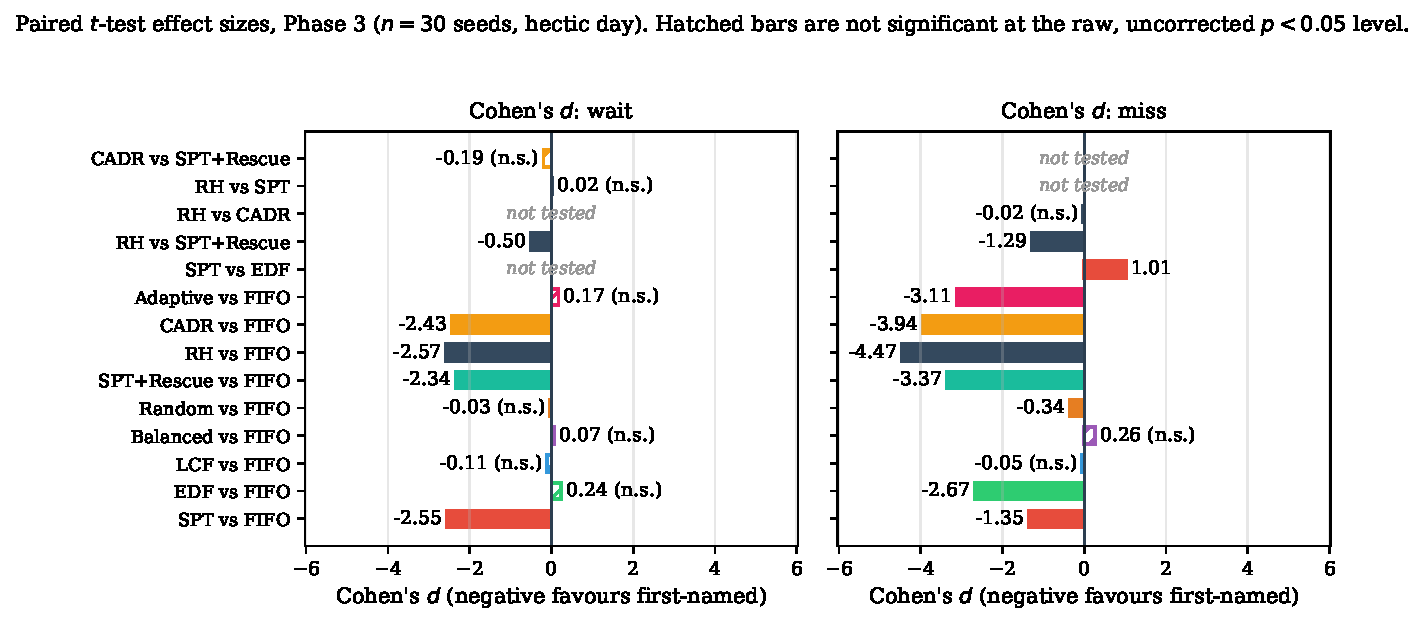
\includegraphics[width=0.98\linewidth,height=0.72\textheight,keepaspectratio]{figures/ttest_effects.pdf}
\caption[Paired t-test effect sizes]{Effect sizes for the whole pairwise family, of which Table~\ref{tab:ttests} prints the pre-specified subset: Cohen's $d$ for average wait (left) and miss rate (right). Negative bars favour the first-named scheduler; hatched bars are not significant at the raw, uncorrected $p<0.05$ level, and pairs without a pre-specified hypothesis for a metric are marked ``not tested''. The headline RH vs CADR miss comparison is non-significant on the paired test, without establishing equivalence, while RH vs FIFO shows the largest miss effect in the study. The shading is the uncorrected verdict, so \HolmRemoved{} bars render solid without surviving the Holm-Bonferroni family-wise correction: RH's wait advantage over SPT+Rescue ($d=\RHRescueWaitD$, raw $p=\RHRescueWaitP$) and Random's lower miss than FIFO ($d=\RandomFIFOmissD$, raw $p=\RandomFIFOmissP$). Defer to the table, not this figure, for every corrected verdict.}
\label{fig:ttest-effects}
\end{figure}
\end{landscape}

Figure~\ref{fig:ttest-effects} presents the same comparisons graphically. The $p$-values are computed from the exact Student $t$-distribution for the paired differences ($\mathrm{df}=n-1$), so they match an independent recomputation (\texttt{scipy.stats.ttest\_rel}); a Wilcoxon signed-rank test gives raw $p<0.05$ for every Holm-significant result, so the conclusions are not artefacts of the normality assumption. Applying the same Holm step-down to the Wilcoxon $p$-values leaves \WilcoxHolmNSig{} of the \HolmNSig{}, so the distribution-free test agrees with the $t$-test family on which comparisons survive. The full pairwise family comprises \HolmFamily{} comparisons, of which Table~\ref{tab:ttests} prints the pre-specified subset; the Holm-Bonferroni step-down correction is applied over the whole family, not over the printed rows, to control the family-wise error rate. Of the \HolmUncorrSig{} comparisons significant at the uncorrected $0.05$ level, \HolmNSig{} remain significant after the correction (the largest surviving $p$-value is below $0.001$), so the correction removes \HolmRemoved{} of them. Both are printed in Table~\ref{tab:ttests} and marked with $^\dagger$ rather than reported as headline findings: RH's wait advantage over SPT+Rescue, and Random's lower miss than FIFO. The wait difference between EDF and FIFO, and the LCF and Balanced comparisons against FIFO, are not significant even before correction, and no claim about any of them is made in this thesis beyond that. Tests reported elsewhere in this chapter are neither members of this family nor included in these counts, and are stated uncorrected. That applies in particular to the three significant tests drawn from the availability and prior sweeps (Section~\ref{ssec:availability-model-sensitivity}), each of which carries a $p$-value well below the smallest threshold a correction over a family of this size could impose, so no conclusion drawn from them turns on the distinction.

The statistical comparison supports the following conclusions.

SPT achieves the lowest wait among the baseline policies under capacity saturation, with no significant paired wait difference from RH. Under hectic overload ($\sim$950 jobs, $\rho>1$), SPT achieves the lowest baseline wait (RH's mean is marginally higher, and the paired test over the same 30 seeds cannot separate the two: $t=\RHSPTwaitT$, $p=\RHSPTwaitP$, $d=\RHSPTwaitD$) but is now significantly outperformed by EDF on miss (\SPTmiss\% vs \EDFmiss\%, $d=\SPTEDFmissD$, $p<0.001$): the two are no longer statistically tied on miss. The effect vs FIFO is large on both metrics.

SPT+Rescue achieves a notably lower miss rate than SPT (\RescueMiss\% vs \SPTmiss\%) but at higher wait (\RescueWait~min vs \SPTwait~min). Under full saturation ($\rho>1$), the rescue tier reorders urgent jobs ahead of the normal SPT queue but cannot prevent all misses caused by the $C_{\max}=5$ concurrency ceiling; promoting urgent jobs displaces normal-tier jobs, adding wait while still reducing net miss relative to bare SPT. The lower mean miss also yields a larger Cohen's $d$ vs FIFO ($d=\RescueFIFOmissD$) than bare SPT ($d=\SPTFIFOmissD$), even though SPT+Rescue's miss rate varies more across seeds than SPT's. SPT+Rescue still provides a very large improvement over FIFO/LCF/Balanced on both metrics.

EDF now achieves significantly lower miss than SPT ($d=\SPTEDFmissD$, $p<0.001$) and carries a higher mean wait than FIFO that the paired test does not resolve ($d=\EDFFIFOwaitD$, $p=\EDFFIFOwaitP$): its deadline ordering helps on miss, while reordering the queue around deadlines rather than job length buys no wait advantage at all over the deadline-oblivious baseline. EDF's mean tardiness (\EDFtard~min) remains low relative to the deadline-oblivious policies, though it no longer leads the deadline-aware group: the Adaptive hybrid now posts lower tardiness (\AdaptiveTard~min vs \EDFtard~min), while CADR (\CADRtard~min) and SPT+Rescue (\RescueTard~min) sit just above EDF (Section~\ref{sec:ablation-analysis}).

RH has the lowest miss-rate point estimate under hectic saturation (\RHMiss\%, with no significant paired difference from CADR's in the 30-seed test, as shown below) while its mean wait (\RHWait~min) is in the lowest tier, with no significant paired wait difference from SPT (\SPTwait~min; $t=\RHSPTwaitT$, $p=\RHSPTwaitP$) and numerically lower than SPT+Rescue (\RescueWait~min). RH's miss advantage over SPT+Rescue survives Holm correction ($d=\RHRescueMissD$, $p<0.001$); its wait advantage, while numerically favourable, has a raw $p=\RHRescueWaitP$ that does \emph{not} survive the family-wise correction (Table~\ref{tab:ttests}), so RH is best described as significantly better than SPT+Rescue on miss and comparable to it on wait, rather than dominant on both metrics. Versus FIFO both gaps are large and significant (miss $d=\RHFIFOmissD$, wait $d=\RHFIFOwaitD$, both $p<0.001$), and RH's operational cost is within roughly 1\% of SPT+Rescue (Section~\ref{ssec:objective-weight-sensitivity}). RH's mean tardiness (\RHtard~min) is not only substantially higher than EDF's (\EDFtard~min) but now exceeds even the deadline-oblivious FIFO baseline (\FIFOtard~min): its urgent tier promotes a tight job only in roughly the last service time before its deadline, and a tight job that misses that window is demoted behind the loose backlog, so under this workload the jobs RH misses are missed by more than FIFO's, even though RH misses far fewer jobs overall.

CADR achieves near-RH miss (\CADRmiss\%) while cutting RH's mean tardiness by \CADRtardReduction\% (\CADRtard~min vs \RHtard~min). CADR's critical-ratio triage promotes at-risk jobs earlier than RH's urgent tier (at $\mathrm{CR}_j \leq 3$ rather than only when a job cannot wait for the next slot), so fewer tight jobs fall into the demoted tier and its misses are mostly loose jobs finishing modestly late. At Phase~3 hectic load, CADR has a lower miss point estimate than SPT+Rescue (\CADRmiss\% vs \RescueMiss\%; no paired miss test between them is in the pre-specified family) at a wait the paired test cannot separate (\CADRwait~min vs \RescueWait~min; $t=\CADRRescueWaitT$, $p=\CADRRescueWaitP$, $d=\CADRRescueWaitD$) and comparable tardiness (\CADRtard~min vs \RescueTard~min): CADR's advantage over SPT+Rescue is concentrated on miss rate rather than a joint improvement on both QoS metrics. The paired RH--CADR miss comparison is not significant ($t=\RHCADRmissT$, $p=\RHCADRmissP$; RH \RHMiss\% vs CADR \CADRmiss\%). Its 95\% interval for the RH-minus-CADR difference is [\RHCADRmissMDLo, \RHCADRmissMDHi] percentage points, so it does not establish equivalence; the choice between the two proposed schedulers can also consider tardiness: RH holds the lower miss point estimate, while CADR has substantially lower mean lateness. Given the unresolved baseline miss difference and CADR's lower tardiness, CADR is the recommended default. RH's miss lead is a point estimate at baseline, becomes significant only at the scarcer $\times 0.75$ availability scale, and reverses under the eased and data-ordered availability settings (Section~\ref{ssec:availability-model-sensitivity}), so RH is the specialist for the scarce baseline regime when the lowest miss count is what matters. For operators who prioritise queue wait, SPT is the natural choice (tied with RH at the hectic baseline and lower elsewhere); RH's wait edge over CADR is an untested point estimate.

The Adaptive queue-pressure EDF-SPT hybrid lands in the mid-tier (\AdaptiveMiss\% miss, \AdaptiveWait~min wait, \AdaptiveTard~min tardiness). Its queue-pressure rule widens the urgent tier to every positive-laxity job once the backlog exceeds the pressure threshold $P$, so at any scheduling event with more than $P$ queued jobs it orders nonnegative-laxity jobs by deadline with hopeless demotion. This betters plain EDF (\EDFmiss\%) and SPT (\SPTmiss\%) on miss and sits about one percentage point below SPT+Rescue (\RescueMiss\%), a gap that no pre-specified test in this study addresses; its mean wait sits slightly above FIFO's rather than matching it, because EDF ordering carries no throughput benefit. CADR has lower miss and wait point estimates than Adaptive at comparable cost (the miss gap is borderline and uncorrected, outside the pre-specified family), though Adaptive holds the lowest mean tardiness of all ten policies (\AdaptiveTard~min), confirming that the adaptive SPT-EDF hybrid design is sound but the proposed RH and CADR policies are stronger on the primary QoS metrics.

Finally, FIFO, LCF, and Balanced incur the highest miss rates. These schedulers carry no deadline information; under saturation tight-deadline jobs queued behind loose-deadline jobs routinely miss their 1-hour window.

\section{Ablation Analysis}
\label{sec:ablation-analysis}

Table~\ref{tab:ablation} traces the evolutionary chain FIFO $\to$ SPT $\to$ SPT+Rescue $\to$ RH on Phase~3 hectic-day results ($n=30$ seeds), showing how each algorithmic addition changes waiting time, deadline miss rate, and mean tardiness relative to the previous step. EDF is included as an alternative single-criterion branch off FIFO (a deadline-driven sibling of the shortest-job-first SPT), isolating which design ingredient, shortest-job-first ordering or deadline awareness, drives each metric. CADR and the CADR-order-only (CADR-OO) ablation variant are included to show the contribution of the cost-aware placement component, and the Adaptive queue-pressure EDF-SPT hybrid is included as an alternative hybrid branch. Cohen's $d$ is computed against FIFO for every row except SPT+Rescue, which is compared with SPT (the step-wise RH versus SPT+Rescue effect is in Table~\ref{tab:ttests}): positive $d$ indicates an increase (worse) relative to the comparison policy, negative $d$ indicates a decrease (better). Figure~\ref{fig:ablation-waterfall} plots the three metrics across the chain, making the per-step trade-offs visible at a glance.

\begin{table}[htbp]
\centering
\caption[Ablation analysis: evolutionary chain]{Ablation analysis: evolutionary chain on Phase~3 hectic day ($n=30$ seeds, $C_{\max}=5$, $\sim$950 jobs/day). Cohen's $d$ for SPT, EDF, RH, CADR, and Adaptive is relative to FIFO; for SPT+Rescue it is relative to SPT. The RH and CADR comparisons against SPT+Rescue are reported in Table~\ref{tab:ttests} and the Phase~3 statistics (Section~\ref{sec:phase-3-statistical-validation}).}
\label{tab:ablation}
\resizebox{\linewidth}{!}{\begin{tabular}{lrrrrr}
\toprule
\textbf{Scheduler} & \textbf{Avg Wait (min)} & \textbf{Miss \%} & \textbf{Avg Tardiness (min)} & \textbf{Cohen $d$ (wait)} & \textbf{Cohen $d$ (miss)} \\
\midrule
FIFO & 167.93 & 24.43 & 26.01 & -- & -- \\
SPT & 141.45 & 18.96 & 12.02 & -2.552 & -1.351 \\
EDF & 170.22 & 14.71 & 5.16 & 0.242 & -2.668 \\
SPT+Rescue & 146.32 & 13.56 & 5.89 & 0.518 & -1.402 \\
\textbf{RH} (proposed) & 141.70 & 9.60 & 31.84 & -2.571 & -4.467 \\
\textbf{CADR} (proposed) & 144.66 & 9.68 & 5.95 & -2.430 & -3.936 \\
Adaptive (EDF-SPT hybrid) & 169.67 & 12.62 & 4.91 & 0.173 & -3.109 \\
\midrule
CADR-order-only & 145.96 & 10.16 & 6.59 & -- & -- \\
\bottomrule
\end{tabular}
}
\end{table}

\begin{landscape}
\begin{figure}[H]
\centering
\captionsetup{font=small,skip=6pt}
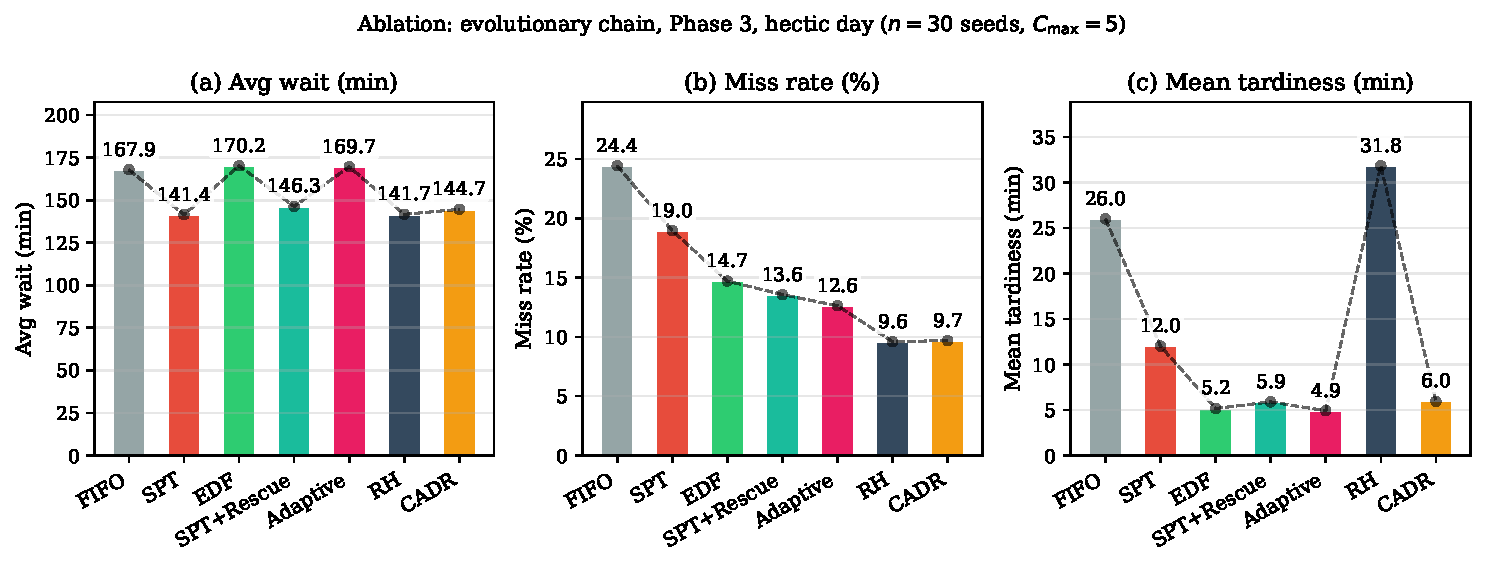
\includegraphics[width=0.98\linewidth,height=0.72\textheight,keepaspectratio]{figures/ablation_waterfall.pdf}
\caption[Ablation waterfall across the design chain]{Ablation waterfall: average wait (a), miss rate (b), and mean tardiness (c) for each scheduler in the evolutionary chain. Each step along the chain adds one algorithmic ingredient. SPT improves both wait and miss over FIFO; EDF cuts miss and tardiness but leaves wait at FIFO level; SPT+Rescue recovers deadline awareness while retaining most of SPT's wait advantage; the Adaptive hybrid (plotted alongside the main chain) widens the rescue idea's urgent tier under queue pressure, with a miss rate slightly below SPT+Rescue's at EDF-like tardiness, though its wait reverts to FIFO level; RH then improves miss significantly and wait numerically over SPT+Rescue (the wait gain does not survive Holm correction), at the price of high tardiness on the jobs it sacrifices; CADR trades a marginal wait increase for a large tardiness reduction (\RHtard{} to \CADRtard\,min) at near-identical miss.}
\label{fig:ablation-waterfall}
\end{figure}
\end{landscape}

The ablation chain isolates the contribution of each design ingredient. The first step, SPT over FIFO, shows that shortest-job-first ordering produces a large reduction in waiting time ($d$ vs FIFO from Table~\ref{tab:ttests}) and a statistically significant miss reduction, confirming that shortest-job-first ordering benefits both metrics simultaneously under saturation. The alternative branch, EDF over FIFO, shows that pure earliest-deadline ordering cuts the miss rate even more than SPT does ($d=\EDFFIFOmissD$ vs $d=\SPTFIFOmissD$) but leaves waiting time at or slightly above FIFO's ($d=\EDFFIFOwaitD$, $p=\EDFFIFOwaitP$, not significant even before correction). Contrasting the EDF and SPT branches therefore isolates the two design ingredients: deadline awareness alone is sufficient to reduce misses under saturation, whereas the wait-time benefit comes specifically from shortest-job-first ordering. This motivates the hybrid designs, which seek both effects at once. EDF's mean tardiness (\EDFtard~min) remains low relative to the deadline-oblivious policies, because its deadline ordering ensures even missed jobs are missed by a small amount, though it no longer leads the deadline-aware group on this metric (the Adaptive hybrid posts lower tardiness here, \AdaptiveTard~min, while CADR and SPT+Rescue sit just above EDF).

The step from SPT to SPT+Rescue shows that the laxity rescue mechanism cuts the mean miss rate substantially (\RescueMiss\% vs \SPTmiss\%, reflected in a larger Cohen $d$ vs FIFO of \RescueFIFOmissD{} against \SPTFIFOmissD{} for SPT), although its miss rate varies more across seeds than SPT's, and it increases mean waiting time because urgent-tier promotions displace short normal-tier jobs. The step from SPT+Rescue to RH improves miss significantly and wait numerically (Table~\ref{tab:ttests}: $d=\RHRescueWaitD$ wait, which does not survive Holm correction, $d=\RHRescueMissD$ miss vs SPT+Rescue); plain SPT also improves both relative to FIFO, but at a far higher miss level. Replacing the fixed laxity threshold with timeline-derived urgency restores SPT shortest-job-first ordering for jobs with slack, cutting wait back to SPT-level; simultaneously, hopeless-demotion (demoting jobs projected to miss under the mean-service estimate in favour of jobs projected to meet their deadlines) combined with precise forward-simulation urgency cuts miss below SPT+Rescue's fixed-threshold approach. However, RH's late promotion of tight jobs, which then fall into its demoted tier, increases mean tardiness relative to SPT+Rescue (\RHtard~min vs \RescueTard~min): jobs that are pushed to the back are missed by substantially more.

CADR at Phase~3 hectic load has a lower miss point estimate than SPT+Rescue (\CADRmiss\% vs \RescueMiss\%; no paired miss test is in the pre-specified family) at essentially the same wait (\CADRwait~min vs \RescueWait~min) and comparable tardiness (\CADRtard~min vs \RescueTard~min); the advantage over SPT+Rescue is concentrated on miss rate rather than a joint improvement on both metrics. CADR achieves near-RH miss (\CADRmiss\% vs \RHMiss\%) while cutting RH's mean tardiness substantially (\CADRtard~min vs \RHtard~min), because its critical-ratio triage promotes at-risk jobs earlier, so fewer tight jobs are demoted behind the loose backlog. RH retains the lowest miss point estimate, though not significantly below CADR's. These are complementary designs, not a linear ``each step better'' chain; because the paired baseline miss test does not separate them and CADR's missed jobs are far less late, CADR is the recommended default and RH the specialist for the scarce baseline regime (Section~\ref{ssec:choosing-between-rh-and-cadr}).

The CADR-order-only (CADR-OO) ablation retains the three-tier critical-ratio ordering but replaces cost-aware node selection with fastest-available-node placement, yielding \CADROOmiss\% miss and \CADROOtard~min tardiness, vs CADR's \CADRmiss\% and \CADRtard~min. Removing cost-aware placement therefore makes no detectable difference to QoS (\CADROOmiss\% vs \CADRmiss\% on miss, and \CADROOtard~min vs \CADRtard~min on tardiness, all within seed-to-seed noise, with tardiness marginally lower without it). This is expected: operational cost headroom is structurally small in this fleet (a marginal, near-noise gap across policies), so optimising node selection for cost does not move the QoS metrics, and CADR's QoS comes from its critical-ratio ordering.

Lastly, the Adaptive queue-pressure hybrid achieves lower miss (\AdaptiveMiss\%) than pure EDF (\EDFmiss\%) and about one percentage point below SPT+Rescue (\RescueMiss\%), with EDF-like low tardiness (\AdaptiveTard~min). These observed results place Adaptive below both SPT+Rescue and EDF on miss point estimate, but no pressure-rule ablation isolates how much of that difference comes from tier widening. It has higher miss and wait point estimates than both proposed schedulers, with no paired test between them: RH (\RHMiss\% miss) and CADR (\CADRmiss\% miss). Tardiness runs the other way, with Adaptive lowest of the ten (\AdaptiveTard~min). The observed miss point estimates put the two proposed schedulers below Adaptive on this workload; the contribution of Adaptive's pressure rule remains unisolated.


\subsection{Capacity Lower Bound}
\label{ssec:capacity-lower-bound}

To situate the Phase~3 miss rates against what any policy could achieve, two brackets are computed on the expected-service hectic instances (the same 30 job streams, each job granted its fastest GPU's mean execution time and zero provisioning delay). First, a certified window-capacity bound: for any window $[s,t]$, the jobs submitted at or after $s$ with deadlines at or before $t$ must fit their total work into $C_{\max}(t-s)$ machine-seconds, so any excess implies unavoidable misses under \emph{every} policy, clairvoyant or not. Across all 30 seeds this bound certifies \CapBoundMeanPct\% unavoidable misses (maximum \CapBoundMaxMisses{} jobs in any seed): the tight-deadline stream alone never exceeds fleet capacity, and the loose eight-hour windows spread the remaining demand far below it. Second, a constructive clairvoyant relaxation: non-preemptive EDF with full hindsight on the same relaxed instances schedules every job on time in every seed (\RelaxEDFMeanPct\% miss). The certificate is one-sided and deterministic: it bounds the expected-service instance, not individual stochastic realisations, whose provisioning and service draws can and do produce misses; that residual is precisely what the simulator measures. The offline-relaxed optimum is therefore exactly zero misses, and no reachable-optimum gap can be quoted against it; instead, the observed miss rates measure the \emph{price of real operation}: online arrivals (Section~\ref{sec:computational-complexity}), non-preemptive dispatch on a heterogeneous fleet, stochastic provisioning delays, and stochastic service times. RH's \RHMiss\% is the smallest measured price among the ten policies as a point estimate (CADR's paired miss difference is not significant in the 30-seed test), and the concurrency study (Section~\ref{ssec:concurrency-limit-sensitivity}) shows RH's residual falling to about 2\% at $C_{\max}=7$ and reaching zero at $C_{\max}=10$, consistent with the relaxation's verdict that baseline capacity is sufficient in expectation. The computation is reproducible via \texttt{CGRSP/phase3\_capacity\_bound.py}.

\subsection{Classical and Learned Baselines}
\label{ssec:classical-and-learned-baselines}

The main comparison in Section~\ref{sec:phase-3-statistical-validation} uses the ten policies of Chapter~\ref{chap:system}. Five further baselines are run on the same 30 seeds, job count, arrival rate, concurrency limit and deadline split: HEFT, min-min, max-min, a shallow tabular bandit, and a uniform random-arm control for that bandit. For independent jobs, HEFT reduces to longest-average-job-first ordering with earliest-finish-time placement, and min-min repeatedly takes the job with the smallest earliest-completion time; both are described in Section~\ref{sec:heterogeneous-machine-scheduling}. The bandit selects among four arms (FIFO, SPT, EDF and SPT+Rescue), is trained for 15 episodes on seeds 500 to 514, and is evaluated with exploration switched off on seeds 0 to 29, so no evaluation seed appears in its training set. The random-arm control draws one of the same four arms uniformly at every decision. Table~\ref{tab:baselines} reports the three primary metrics.

\begin{table}[htbp]
\centering
\caption[Classical and learned baselines]{Classical and learned baselines on the Phase~3 hectic day ($n=30$ seeds, $\sim$950 jobs/day, $C_{\max}=5$, $\lambda=0.100$ j/s, 20\% tight 1h / 80\% loose 8h deadlines). HEFT and max-min produce identical values on every seed and every metric, so they are shown as one row. Mean tardiness is over completed jobs, with zero for on-time jobs. Bold marks the column minimum; the paired tests are in the text.}
\label{tab:baselines}
\begin{tabular}{lrrr}
\toprule
\textbf{Scheduler} & \textbf{Avg Wait (min)} & \textbf{Miss \%} & \textbf{Mean Tardiness (min)} \\
\midrule
HEFT $=$ MaxMin & 191.77 & 29.90 & 39.53\\
MinMin & \textbf{141.42} & 19.06 & 24.64\\
Bandit & 169.44 & 25.45 & 24.66\\
Bandit-random & 157.82 & 13.57 & \textbf{5.02}\\
FIFO & 167.93 & 24.43 & 26.01\\
RH & 141.70 & \textbf{9.60} & 31.84\\
CADR & 144.66 & 9.68 & 5.95\\
\bottomrule
\end{tabular}

\end{table}

The table separates the baselines sharply. HEFT and max-min are indistinguishable on this fleet: their per-seed values are identical on all six metrics, and the 30-comparison Holm family in the JSON therefore contains six duplicate comparisons, leaving 24 unique ones. HEFT's longest-average-job-first order is the reverse of SPT's, and max-min records the same values here; both record the highest wait (191.77~min) and miss rate (29.90\%) in the table, well above FIFO's \FIFOwait~min and \FIFOmiss\%.

MinMin records the lowest wait point estimate in the table (141.42~min). The paired test does not separate it from RH's \RHWait~min ($p_{\text{Holm}}=0.8904$, $d=-0.0283$), and its difference from CADR's \CADRwait~min is not significant at the raw or corrected level ($p=0.0831$, $p_{\text{Holm}}=0.3326$). Its miss rate is 19.06\%, however, significantly worse than RH's \RHMiss\% ($d=+2.4006$) and CADR's \CADRmiss\% ($d=+2.1770$), each $p<0.001$ after correction. MinMin therefore reaches the proposed schedulers on wait but not on deadline compliance.

The shallow bandit is a null result in this design. Its miss rate is 25.45\% against FIFO's \FIFOmiss\% ($p=0.1213$), and its wait is 169.44~min against \FIFOwait~min ($p=0.3383$); neither difference is significant, while RH and CADR are both significantly better than it on miss ($p<0.001$). The uniform random-arm control records a lower miss rate than the trained bandit (13.57\% against 25.45\%), so this experiment provides no evidence that the learned arm selection improves on chance. The result is specific to a tabular, episode-level bandit with four arms and a shallow training budget on this workload; it is not evidence about deep reinforcement learning, which remains open (Chapter~\ref{chap:conclusion}).

\section{Sensitivity Analysis}
\label{sec:sensitivity-analysis}

\subsection{Day-Type Sensitivity (\texorpdfstring{$C_{\max}=5$}{Cmax=5})}
\label{ssec:day-type-sensitivity-c-max-5}

Table~\ref{tab:sensitivity} summarises the average waiting time and deadline miss rate for all schedulers across four operationally calibrated day types at $C_{\max}=5$ (30 seeds per day type). Figure~\ref{fig:sensitivity} shows the full results. This study uses full 30-seed replication at every day type, matching the Phase~3 hectic-day protocol (Section~\ref{sec:phase-3-statistical-validation}); the surge-day anticipation benefit is additionally isolated at $n=30$ in the dedicated reservation study (Section~\ref{ssec:anticipation-reservation-sensitivity}).

\begin{landscape}
\begin{figure}[H]
\centering
\captionsetup{font=small,skip=6pt}
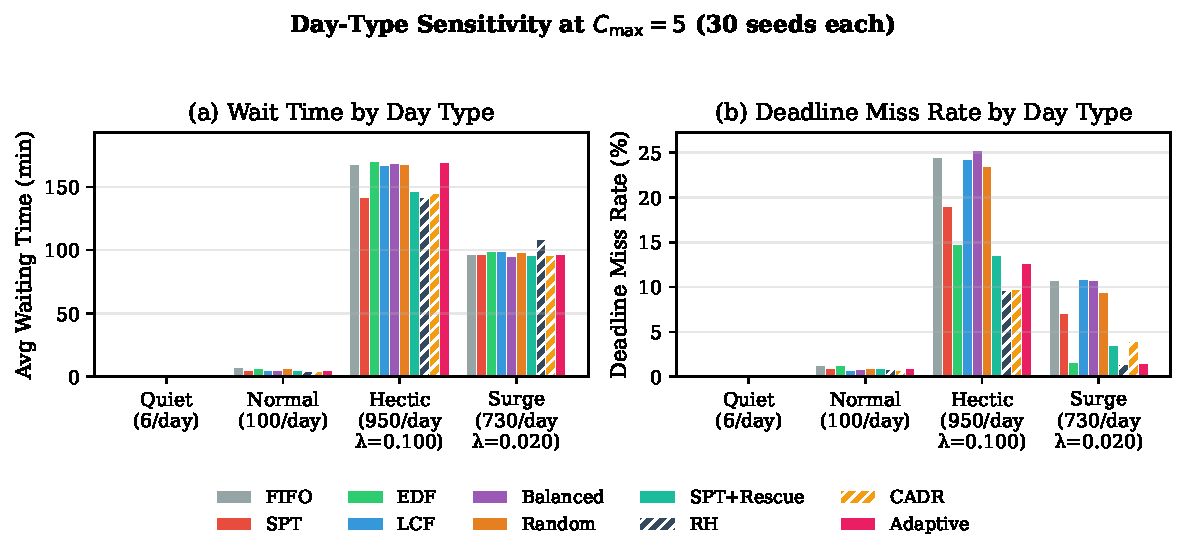
\includegraphics[width=0.98\linewidth,height=0.72\textheight,keepaspectratio]{figures/sensitivity_heatmap.pdf}
\caption[Day-type sensitivity results]{Day-type sensitivity at $C_{\max}=5$ (30 seeds each, 20\% tight 1h / 80\% loose 8h deadlines): (a) average waiting time and (b) deadline miss rate. Quiet days: 0\% miss all schedulers. Normal days: near-zero miss. Hectic days ($\sim$950 jobs, $\rho>1$): RH lowest miss (\SensHecRHmiss\%, \SensHecRHwait~min wait, tied with SPT for lowest wait); CADR near-RH miss (\SensHecCADRmiss\%, \SensHecCADRwait~min wait); SPT lowest-tier wait, tied with RH (\SensHecSPTwait~min, \SensHecSPTmiss\% miss); FIFO/LCF/Balanced \FIFOmiss\% to \Balancedmiss\% miss. Surge days: Adaptive, EDF, and RH form the lowest miss tier, within half a percentage point of one another (no paired test is computed for the day-type sweep) (\SensSrgAdaptiveMiss\% / \SensSrgEDFmiss\% / \SensSrgRHmiss\%); SPT+Rescue \SensSrgRescueMiss\%; FIFO, LCF, and Balanced 10 to 11\%.}
\label{fig:sensitivity}
\end{figure}
\end{landscape}

\begin{table}[H]
\centering
\caption[Day-type sensitivity summary]{Day-type sensitivity: avg wait (min) / miss\% at $C_{\max}=5$, 20\% tight 1h / 80\% loose 8h deadlines ($n=30$ seeds each). All ten schedulers are shown across the four day types. Bold marks the scheduler with the lowest miss rate in the hectic and surge columns (the whole wait / miss cell), not the lowest wait.}
\label{tab:sensitivity}
\begingroup\setlength{\tabcolsep}{9pt}
\begin{tabular}{lcccc}
\toprule
& \multicolumn{4}{c}{\textbf{Avg Wait (min) / Miss \%}} \\
\cmidrule(lr){2-5}
\textbf{Scheduler} & \textbf{Quiet} & \textbf{Normal} & \textbf{Hectic} & \textbf{Surge} \\
\midrule
SPT & 0.5 / 0.0 & 5.0 / 1.0 & 141.4 / 19.0 & 96.7 / 7.0 \\
LCF & 0.5 / 0.0 & 4.7 / 0.7 & 166.9 / 24.2 & 98.8 / 10.8 \\
Balanced & 0.5 / 0.0 & 5.1 / 0.8 & 168.6 / 25.2 & 94.9 / 10.7 \\
FIFO & 0.7 / 0.0 & 7.2 / 1.2 & 167.9 / 24.4 & 96.4 / 10.7 \\
EDF & 0.5 / 0.0 & 6.2 / 1.2 & 170.2 / 14.7 & 99.2 / 1.6 \\
Random & 0.6 / 0.0 & 6.7 / 0.9 & 167.7 / 23.4 & 98.0 / 9.4 \\
SPT+Rescue & 0.5 / 0.0 & 5.0 / 1.0 & 146.3 / 13.6 & 95.4 / 3.5 \\
RH & 0.5 / 0.0 & 4.3 / 0.8 & \textbf{141.7 / 9.6} & \textbf{108.8 / 1.3} \\
CADR & 0.5 / 0.0 & 4.5 / 0.7 & 144.7 / 9.7 & 95.4 / 4.0 \\
Adaptive & 0.5 / 0.0 & 5.0 / 1.0 & 169.7 / 12.6 & 96.4 / 1.5 \\
\bottomrule
\end{tabular}
\endgroup

\end{table}

Quiet and normal days show near-zero miss for all schedulers: at $\sim$6 and $\sim$100 jobs/day, load is very light ($\rho \ll 1$), and queue wait is sub-minute (quiet) and under 10~min (normal). On hectic days ($\sim$950 jobs, $C_{\max}=5$, $\rho>1$), capacity saturation dominates. RH achieves the lowest miss in this 30-seed sample (\SensHecRHmiss\%, \SensHecRHwait~min wait, nearly identical to SPT's); CADR achieves near-RH miss (\SensHecCADRmiss\%) with lower tardiness than RH; SPT achieves a lowest-tier wait (\SensHecSPTwait~min, \SensHecSPTmiss\% miss; see Phase~3, Section~\ref{sec:phase-3-statistical-validation}, where $n=30$ seeds finds EDF's hectic-day miss significantly lower than SPT's, $p<0.001$). Deadline-unaware schedulers (FIFO, LCF, Balanced) incur \FIFOmiss\% to \Balancedmiss\% miss.

On surge days, the Adaptive hybrid, EDF, and RH form the lowest miss tier (no paired test is computed for the day-type sweep). Under surge conditions (730 jobs, $\lambda=0.020$ j/s, execution-only offered load $\rho\approx0.30$, below saturation), the slower sustained arrival rate leaves execution capacity to spare between burst windows. Mean waits nevertheless reach roughly \SensSrgDayWaitLo{} to \SensSrgDayWaitHi{}~min (Table~\ref{tab:sensitivity}), because each dispatch holds its slot through a stock-dependent provisioning delay that $\rho$ does not count; these delays hold slots and can build a surge-day queue even when execution-only offered load is below saturation. RH's load-gated anticipation activates here: it reserves a slot for anticipated tight-deadline arrivals and dispatches waiting tight jobs eagerly. This cuts RH surge miss to \SensSrgRHmiss\%, nearly identical to EDF (\SensSrgEDFmiss\%) and the Adaptive hybrid (\SensSrgAdaptiveMiss\%) at the lowest tier, and well below SPT (\SensSrgSPTmiss\%) and SPT+Rescue (\SensSrgRescueMiss\%). Adaptive's ten-job pressure rule widens the urgent tier when the \emph{waiting queue} exceeds that threshold; the reported mean wait includes time after dispatch during provisioning, so it cannot establish how often this rule fires. The surge-day miss result is consistent with EDF-style ordering, but the contribution of pressure widening has not been isolated by a queue-length measurement or ablation. RH pays for this deadline protection with a higher mean wait (\SensSrgRHwait~min), because the reserved slot briefly idles, a trade-off specific to this below-saturation regime (under hectic saturation the load gate disables reservation and no such wait premium appears). The dedicated reservation study (Section~\ref{ssec:anticipation-reservation-sensitivity}, $n=30$ seeds) isolates this anticipation benefit at full replication and confirms it is specific to below-saturation load.

The hectic/surge contrast thus reveals a load-regime boundary: at surge load, EDF, the Adaptive hybrid and RH cluster at the lowest miss, whereas at hectic overload SPT achieves the lowest wait among the baseline policies (tied with RH) but is significantly outperformed on miss by EDF ($p<0.001$) and has a higher miss point estimate than every other deadline-aware policy.

\subsection{Deadline Tightness Sensitivity}
\label{ssec:deadline-tightness-sensitivity}

The deadline tightness study varies the fraction of tight-deadline jobs ($f_{\text{tight}} \in \{10\%,\allowbreak 30\%,\allowbreak 50\%,\allowbreak 70\%,\allowbreak 90\%\}$) under surge-day conditions (the surge-day configuration of Section~\ref{ssec:platform-and-data}, 30 seeds per sweep point). Table~\ref{tab:deadline} and Figure~\ref{fig:deadline} report miss rates across the five tight-deadline fractions.

\begin{table}[htbp]
\centering
\caption[Deadline-tightness sweep]{Deadline-tightness sweep: miss rate (\%) per baseline scheduler at each tight-deadline fraction (surge day, $C_{\max}=5$, $\lambda=0.020$ j/s). Bold marks the row minimum. In the 50\% row that minimum is not a significant winner: EDF's and SPT's values there are not separated by the paired test over the same 30 seeds ($\DlFiftySPTEDFmissP$), so the bold should be read as the smaller of two numbers the study cannot separate.}
\label{tab:deadline}
\begin{tabular}{cccccccc}
\toprule
\textbf{Tight \%} & \textbf{FIFO} & \textbf{SPT} & \textbf{EDF} & \textbf{LCF} & \textbf{Balanced} & \textbf{Random} & \textbf{SPT+Rescue} \\
\midrule
10\% & 5.27 & 3.31 & \textbf{0.62} & 5.29 & 5.21 & 4.61 & 1.41\\
30\% & 16.44 & 10.96 & \textbf{3.45} & 16.59 & 16.35 & 14.19 & 6.99\\
50\% & 27.07 & 18.91 & \textbf{18.34} & 27.34 & 26.86 & 23.56 & 22.10\\
70\% & 37.84 & \textbf{27.56} & 34.64 & 38.23 & 37.48 & 32.39 & 36.46\\
90\% & 48.56 & \textbf{36.74} & 48.16 & 49.08 & 48.18 & 41.80 & 48.67\\
\bottomrule
\end{tabular}

\end{table}

\begin{landscape}
\begin{figure}[H]
\centering
\captionsetup{font=small,skip=6pt}
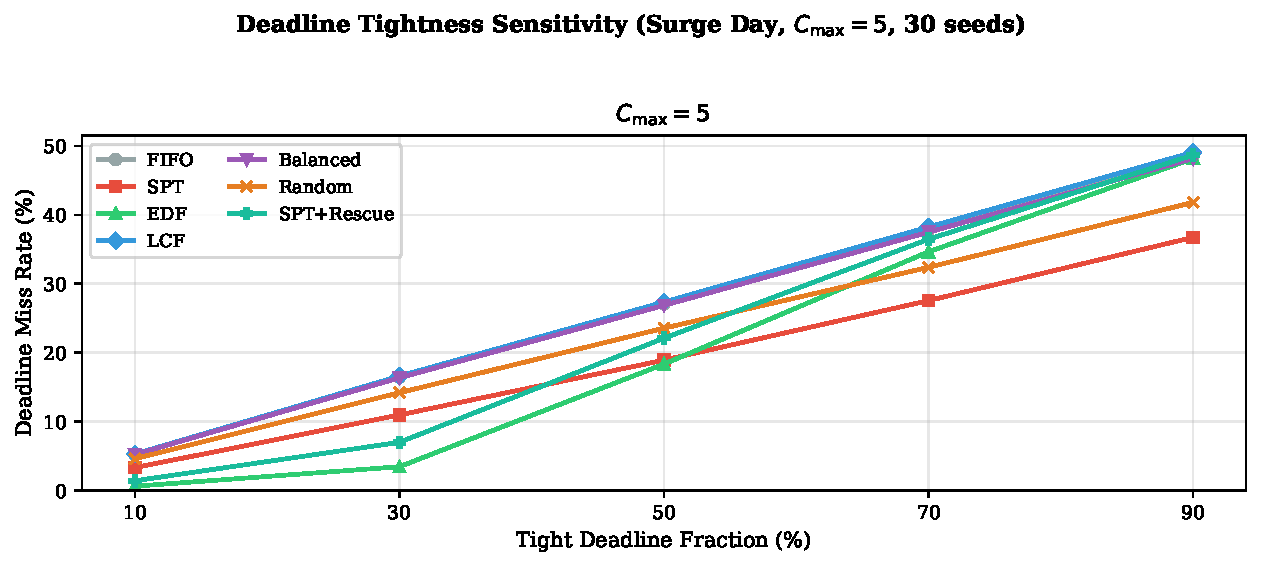
\includegraphics[width=0.98\linewidth,height=0.72\textheight,keepaspectratio]{figures/deadline_sensitivity.pdf}
\caption[Deadline-tightness sensitivity]{Deadline miss rate (\%) vs tight-deadline fraction (surge day, $C_{\max}=5$, 730 jobs, 30 seeds). EDF's miss is significantly lower than SPT's at $f_{\text{tight}} \leq 30\%$ and SPT's is significantly lower at $f_{\text{tight}} \geq 70\%$, while at $f_{\text{tight}} = 50\%$ the paired test does not resolve their difference ($\DlFiftySPTEDFmissP$), so the curves cross over an interval rather than at a point.}
\label{fig:deadline}
\end{figure}
\end{landscape}

No scheduler achieves 0\% miss across all tight-deadline fractions at surge-day load: although execution demand is below saturation, provisioning delays hold each slot and push waits to roughly \SensSrgWaitLo{} to \SensSrgWaitHi{}~min against 1\,h tight deadlines, so tight-deadline misses grow with $f_{\text{tight}}$ and are not removed by any ordering policy tested. Among the seven baseline policies in this sweep (RH, CADR, and Adaptive are not part of it), the EDF-SPT ordering reverses across the sweep, and a paired test at each of the five points locates the reversal rather than leaving it to the point estimates. The test is signed SPT minus EDF, so a positive $t$ favours EDF. EDF's miss is significantly lower at $f_{\text{tight}} = 10\%$ ($t=\DlTenSPTEDFmissT$, $\DlTenSPTEDFmissP$; \DlTenEDFmiss\% vs \DlTenSPTmiss\%) and at $f_{\text{tight}} = 30\%$ ($t=\DlThirtySPTEDFmissT$, $\DlThirtySPTEDFmissP$; \DlThirtyEDFmiss\% vs \DlThirtySPTmiss\%), with SPT+Rescue second-best at both. At $f_{\text{tight}} = 50\%$ the paired test does not resolve their difference ($t=\DlFiftySPTEDFmissT$, $\DlFiftySPTEDFmissP$): EDF's \DlFiftyEDFmiss\% and SPT's \DlFiftySPTmiss\% differ by less than the seed-to-seed variation, so the study names no winner at this point. SPT's miss is then significantly lower at $f_{\text{tight}} = 70\%$ ($t=\DlSeventySPTEDFmissT$, $\DlSeventySPTEDFmissP$; \DlSeventySPTmiss\% vs \DlSeventyEDFmiss\%) and at $f_{\text{tight}} = 90\%$ ($t=\DlNinetySPTEDFmissT$, $\DlNinetySPTEDFmissP$; \DlNinetySPTmiss\% vs \DlNinetyEDFmiss\%), where shortest-job-first ordering completes more jobs before their deadlines expire than deadline ordering does. The operational recommendation follows directly: use EDF or SPT+Rescue when the tight-deadline fraction is low ($f_{\text{tight}} \leq 30\%$) and switch to SPT once most jobs carry tight deadlines ($f_{\text{tight}} \geq 70\%$), with either choice defensible at $f_{\text{tight}} = 50\%$, where the paired test does not resolve their difference.

\subsection{Concurrency Limit Sensitivity}
\label{ssec:concurrency-limit-sensitivity}

The experiments fix $C_{\max}=5$, RunPod's default per-account worker quota; RunPod raises that quota in account-balance tiers (10 workers at \$100, up to 60 at \$900) or on request~\cite{runpod2026maxworkers}, and an operator may also cap concurrency below it for cost control. Table~\ref{tab:cmax_sensitivity} evaluates hectic-day performance ($n=10$ seeds, $\sim$950 jobs/day) across $C_{\max} \in \{3, 5, 7, 10\}$ to show how scheduler rankings shift under alternative provider policies; budgets above five are simulated what-ifs, since the calibration data never exceed five concurrent jobs. Figure~\ref{fig:cmax-sensitivity} plots the resulting saturation curves.

\begin{table}[htbp]
\centering
\caption[Concurrency limit sensitivity]{Concurrency limit sensitivity: avg wait (min) / miss\% on hectic day ($n=10$ seeds, $\sim$950 jobs/day, 20\% tight 1h / 80\% loose 8h deadlines); the $C_{\max}=5$ column therefore differs slightly from the 30-seed Phase~3 means. The \textbf{baseline} column ($C_{\max}=5$) is RunPod's default worker quota; the other columns correspond to tighter operator caps or higher RunPod quota tiers.}
\label{tab:cmax_sensitivity}
\begin{tabular}{lcccc}
\toprule
& \multicolumn{4}{c}{\textbf{Avg Wait (min) / Miss \%}} \\
\cmidrule(lr){2-5}
\textbf{Scheduler} & $C_{\max}=3$ & \shortstack{$C_{\max}=5$ \\ \textbf{(baseline)}} & $C_{\max}=7$ & $C_{\max}=10$ \\
\midrule
FIFO & 387.1\,/\,57.3 & 165.8\,/\,23.7 & 44.7\,/\,6.3 & 8.5\,/\,0.0 \\
SPT & 358.6\,/\,51.6 & 137.6\,/\,17.7 & 38.7\,/\,2.8 & 8.1\,/\,0.0 \\
EDF & 394.4\,/\,51.6 & 168.4\,/\,12.7 & 44.6\,/\,0.0 & 9.0\,/\,0.0 \\
SPT+Rescue & 372.1\,/\,49.7 & 144.7\,/\,13.5 & 39.0\,/\,0.0 & 8.1\,/\,0.0 \\
RH & 364.9\,/\,46.3 & 139.5\,/\,8.5 & 38.5\,/\,2.0 & 13.1\,/\,0.0 \\
CADR & 375.3\,/\,48.4 & 142.8\,/\,9.3 & 38.8\,/\,0.0 & 7.4\,/\,0.0 \\
Adaptive & 395.6\,/\,50.5 & 166.3\,/\,11.5 & 44.1\,/\,0.0 & 8.7\,/\,0.0 \\
\bottomrule
\end{tabular}

\end{table}

\begin{landscape}
\begin{figure}[H]
\centering
\captionsetup{font=small,skip=6pt}
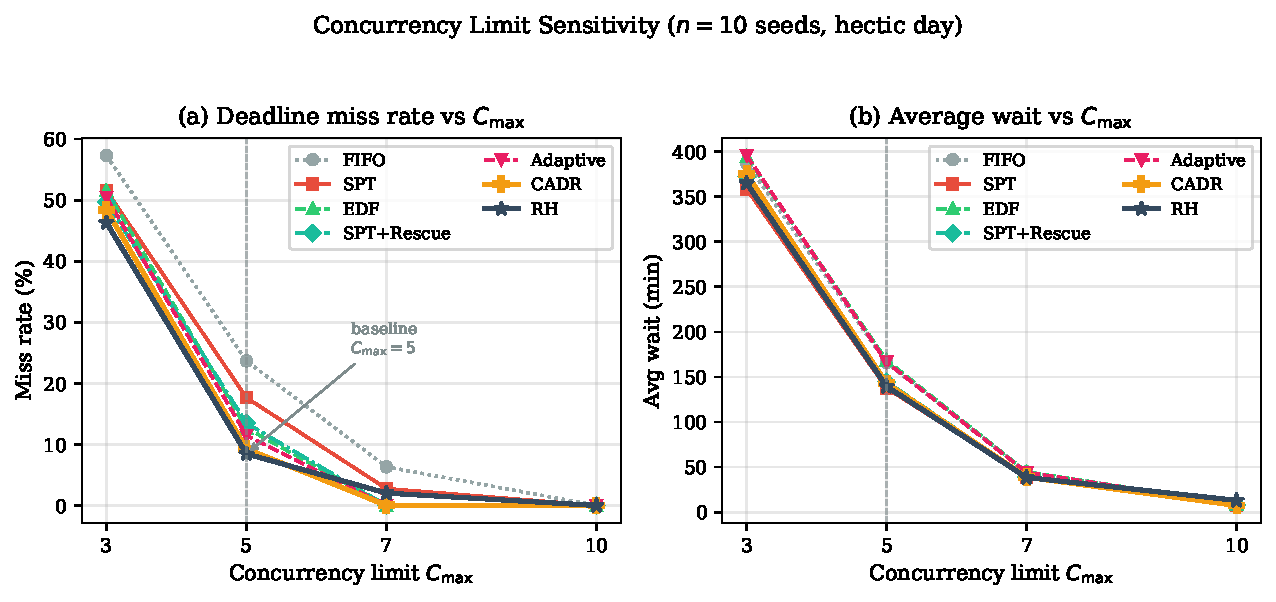
\includegraphics[width=0.98\linewidth,height=0.72\textheight,keepaspectratio]{figures/cmax_sensitivity.pdf}
\caption[Concurrency limit sensitivity]{Concurrency limit sensitivity: miss rate (a) and average wait (b) vs $C_{\max} \in \{3, 5, 7, 10\}$, $n=10$ seeds, hectic day. The dashed vertical line marks the $C_{\max}=5$ baseline. The saturation curve is clearly visible: the largest improvement in miss rate occurs between $C_{\max}=3$ and $C_{\max}=5$; gains are smaller from 5 to 7 and small from 7 to 10, where RH clears its remaining residual and FIFO its remaining \CmaxSevenFIFOmiss\%. At $C_{\max}=7$ the deadline-aware schedulers EDF, SPT+Rescue, CADR, and Adaptive reach near-zero miss (RH retains a small residual), but FIFO still lags at \CmaxSevenFIFOmiss\%, confirming that scheduler choice remains important even with more concurrency. The anomalous rise in RH's markedly higher wait at $C_{\max}=10$ (\CmaxTenRHwait{} against \CmaxTenOtherWaitLo{} to \CmaxTenOtherWaitHi{}~min for the other policies) relative to the other deadline-aware policies reflects the reservation mechanism briefly idling slots under the now-unsaturated load.}
\label{fig:cmax-sensitivity}
\end{figure}
\end{landscape}

At $C_{\max}=3$ (a restrictive provider policy) all schedulers incur high miss rates: with only three concurrent slots for $\sim$950 jobs/day ($\rho \gg 1$), the queue never drains, and even deadline-aware schedulers cannot prevent structural saturation misses. Under such a policy the choice of scheduling algorithm matters less than the concurrency ceiling itself. $C_{\max}=5$ (RunPod's default quota) is the binding operational constraint at hectic-day load: even the best deadline-aware schedulers still miss a substantial fraction of deadlines, whereas raising the budget by two slots to $C_{\max}=7$ brings deadline-aware schedulers to near-zero miss. At $C_{\max}=10$ every scheduler, FIFO included, reaches zero miss on the hectic day; mean waits are then about \CmaxTenOtherWaitLo{} to \CmaxTenOtherWaitHi~min for every policy except RH (\CmaxTenRHwait~min), whose reservation mechanism briefly idles slots under the unsaturated load. The scheduler comparison on miss is therefore decided at the baseline budget and below, and a budget large enough to clear a hectic day needs no scheduler help; the schedulers matter when the budget binds, as it does at the default quota of 5. The returns to added concurrency are diminishing: the miss reduction from $C_{\max}=3$ to $5$ is the largest single step, that from $5$ to $7$ is smaller, and from $7$ to $10$ smaller still. At $C_{\max}=7$ the deadline-aware policies drain the queue fast enough to meet almost every deadline, but FIFO continues to incur clearly elevated miss due to the absence of deadline ordering; only at $C_{\max}=10$ does FIFO also reach zero. This finding is practically relevant: if an operator's concurrency budget were raised to 7, an operator using FIFO would still benefit substantially from switching to a deadline-aware scheduler. Scheduler differences are largest at $C_{\max}=5$: at $C_{\max}=3$ all schedulers converge to near-total saturation, while at $C_{\max} \geq 7$ the deadline-aware schedulers converge to near-zero miss. The default $C_{\max}=5$ baseline therefore maximises the discriminating power of the scheduler comparison, because it is the point where the concurrency budget binds, and it provides the strongest motivation for deploying RH or CADR whenever the budget binds.

\subsection{Rescue Threshold Sensitivity}
\label{ssec:rescue-threshold-sensitivity}

Table~\ref{tab:threshold_sensitivity} sweeps the SPT+Rescue laxity threshold $\theta \in \{60, 180, 300, 600, 1200\}$\,s on hectic-day workload ($n=10$ seeds, $C_{\max}=5$, $\sim$950 jobs/day); Figure~\ref{fig:threshold-sensitivity} plots the sweep. The threshold controls when a job transitions from the normal SPT tier to the urgent EDF tier.

\begin{table}[htbp]
\centering
\caption[SPT+Rescue threshold sensitivity]{SPT+Rescue threshold sensitivity: avg wait (min) and miss\% on hectic day ($n=10$ seeds, $C_{\max}=5$, 20\% tight 1h / 80\% loose 8h deadlines). Minimum miss rate row is \textbf{bold}.}
\label{tab:threshold_sensitivity}
\begin{tabular}{lrr}
\toprule
\textbf{Threshold $\theta$} & \textbf{Avg Wait (min)} & \textbf{Miss \%} \\
\midrule
$\theta=60$\,s & 142.59 & 15.19 \\
$\theta=180$\,s & 142.04 & 11.66 \\
$\theta=300$\,s & 141.82 & 12.01 \\
\textbf{$\theta=600$\,s} (default) & 144.71 & 13.47 \\
$\theta=1200$\,s & 140.51 & \textbf{11.35} \\
\bottomrule
\end{tabular}

\end{table}



\Needspace{5\baselineskip}
Very small $\theta$ ($\leq 60$\,s) degrades SPT+Rescue towards plain-SPT behaviour: with a 60\,s threshold, few jobs enter the rescue tier early enough to be saved, so the mechanism yields the least benefit and the highest miss rate in the sweep (\ThrSixtyMiss\%). Beyond that, miss rate depends weakly and non-monotonically on $\theta$, varying within a narrow band. Across the whole sweep the miss rate stays within a \ThrMissSpread\,percentage-point band: it is highest at $\theta=60$\,s (\ThrSixtyMiss\%), reaches its lowest value at $\theta=180$\,s (\ThrOneEightyMiss\%), and is non-monotonic thereafter (\ThrSixHundredMiss\% at $\theta=600$\,s, \ThrTwelveHundredMiss\% at $\theta=1200$\,s). Mean wait varies only modestly over the sweep (a spread of roughly eight minutes) with no systematic trend in $\theta$. The mechanism is thus not sensitive to the exact threshold within a broad band, because the loose-deadline majority retains ample slack to absorb the reordering, and at $n=10$ the within-band differences are comparable to the sampling noise. It follows that $\theta = 600$\,s is an acceptable default. It is not the miss-minimising value in this $n=10$ sweep (the minimum is \ThrOneEightyMiss\% at $\theta=180$\,s), but because the miss rate varies by only \ThrMissSpread\,percentage points across the entire swept range, the choice of $\theta$ within this band is small relative to the $n=10$ seed noise. The default $\theta=600$\,s keeps mean wait moderate (\ThrSixHundredWait~min) and requires no fine tuning; a tighter $\theta$ around $180$\,s would lower the miss rate by \ThrDefaultGap\,percentage points, a gap that at $n=10$ lies within the noise band and is not separately optimised here (Table~\ref{tab:threshold_sensitivity}).


\begin{landscape}
\begin{figure}[H]
\centering
\captionsetup{font=small,skip=6pt}
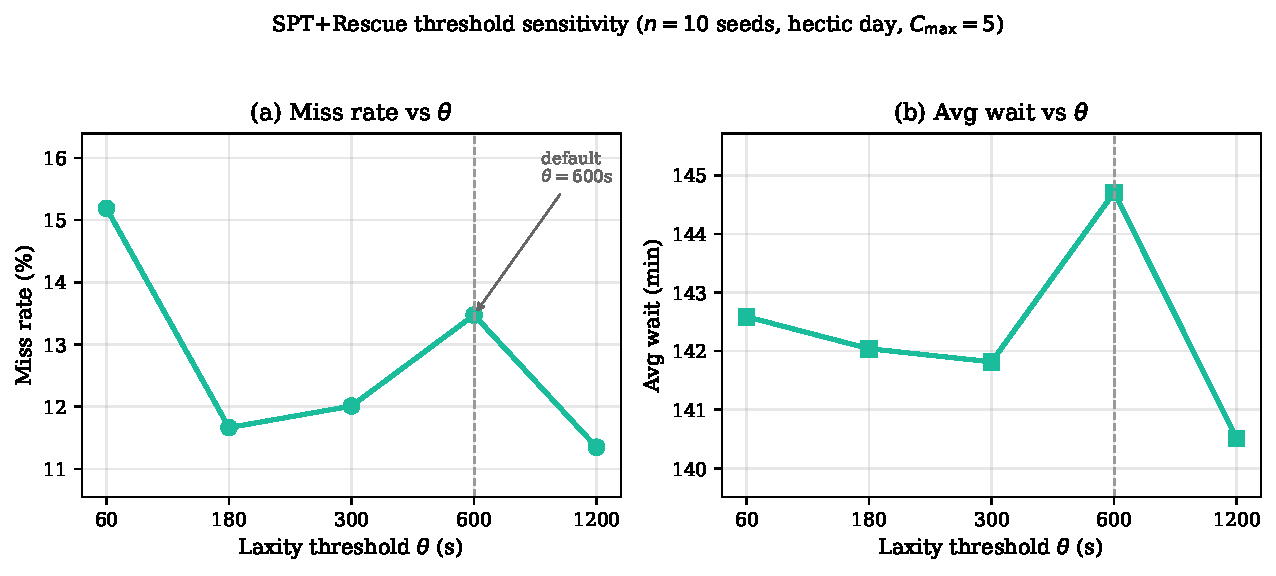
\includegraphics[width=0.98\linewidth,height=0.72\textheight,keepaspectratio]{figures/threshold_sensitivity.pdf}
\caption[SPT+Rescue threshold sensitivity]{SPT+Rescue laxity threshold $\theta$ sensitivity: miss rate (a) and average wait (b) across $\theta \in \{60, 180, 300, 600, 1200\}$\,s. The non-monotone shape of the miss rate curve is directly visible: the minimum is at $\theta=180$\,s; the curve then rises to its second-highest value at $\theta=300$\,s (\ThrThreeHundredMiss\%), dips at the default $\theta=600$\,s (\ThrSixHundredMiss\%), and rises slightly again at $\theta=1200$\,s (\ThrTwelveHundredMiss\%). The total variation across the whole range is \ThrMissSpread\,percentage points, confirming that the mechanism is robust to threshold choice within a broad interval. The dashed line marks the default $\theta=600$\,s.}
\label{fig:threshold-sensitivity}
\end{figure}
\end{landscape}

\subsection{Critical-Ratio Threshold Sensitivity}
\label{ssec:critical-ratio-threshold-sensitivity}

Table~\ref{tab:cr_sensitivity} sweeps the CADR critical-ratio threshold $\mathrm{CR}^*$ on hectic-day workload ($n=10$ seeds, $C_{\max}=5$, $\sim$950 jobs/day); Figure~\ref{fig:cr-sensitivity} plots the sweep. The threshold determines the boundary between the at-risk tier (dispatched EDF) and the safe tier (dispatched SPT); a higher $\mathrm{CR}^*$ promotes more jobs to the at-risk tier.

\begin{table}[htbp]
\centering
\caption[CADR critical-ratio threshold sensitivity]{Critical-ratio threshold sensitivity for CADR: avg wait (min) and miss\% on hectic day ($n=10$ seeds, $C_{\max}=5$). Minimum miss rate row is \textbf{bold}.}
\label{tab:cr_sensitivity}
\begin{tabular}{lrr}
\toprule
\textbf{$CR^{*}$ threshold} & \textbf{Avg Wait (min)} & \textbf{Miss \%} \\
\midrule
$CR^{*}=1.5$ & 142.94 & 11.47 \\
$CR^{*}=2.0$ & 142.34 & 10.14 \\
$CR^{*}=3.0$ & 142.80 & \textbf{9.28} \\
$CR^{*}=5.0$ & 143.94 & 9.96 \\
$CR^{*}=10.0$ & 145.10 & 10.05 \\
\bottomrule
\end{tabular}

\end{table}



\textbf{Critical-ratio sensitivity findings:} the CADR miss rate across the swept $\mathrm{CR}^*$ range has a best value of \CRStarBestMiss\% and a spread of only \CRStarMissSpread\,percentage points, confirming that the threshold is robust. The shipped default $\mathrm{CR}^*=\CRStarBestCR$ is itself the miss-minimising point of the sweep (\CRStarDefaultMiss\%, a gap of \CRStarDefaultGap\,pp to the sweep best), so it requires no tuning in practice; the miss rate is flat for $\mathrm{CR}^*\ge 3$ and rises at $\mathrm{CR}^*\le 2$ (CADR's lead over SPT+Rescue narrows at $\mathrm{CR}^*=2$ and is gone at $\mathrm{CR}^*=1.5$), so the default sits at the edge of the flat region rather than inside a wide plateau.


\begin{landscape}
\begin{figure}[H]
\centering
\captionsetup{font=small,skip=6pt}
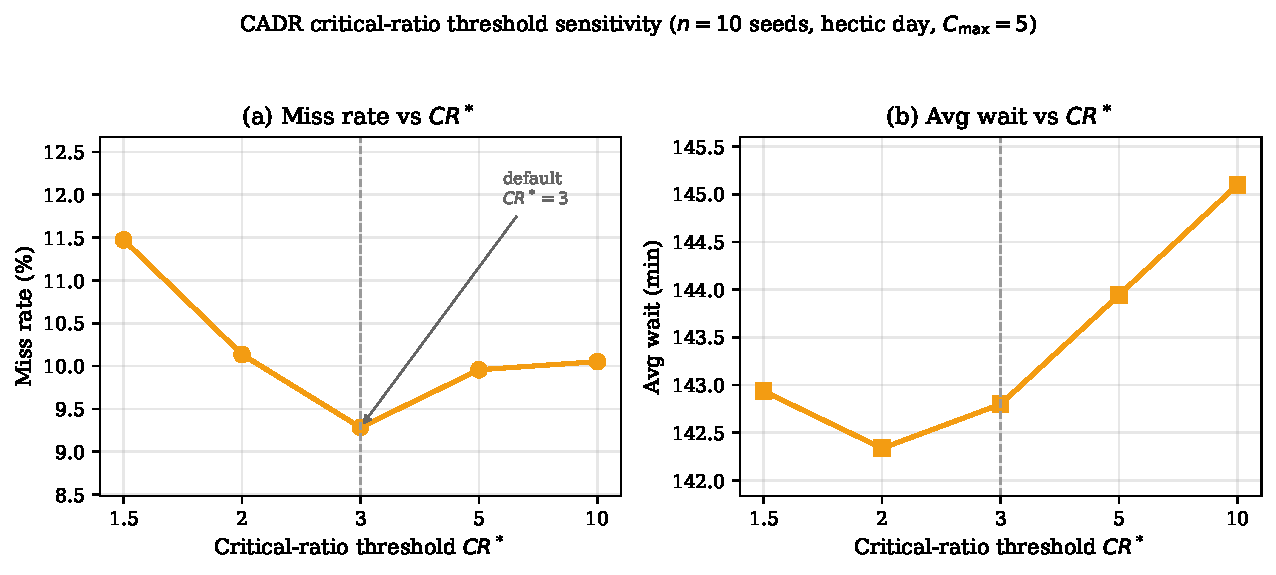
\includegraphics[width=0.98\linewidth,height=0.72\textheight,keepaspectratio]{figures/cr_sensitivity.pdf}
\caption[CADR critical-ratio threshold sensitivity]{CADR critical-ratio threshold $\mathrm{CR}^*$ sensitivity: miss rate (a) and average wait (b) across $\mathrm{CR}^* \in \{1.5, 2.0, 3.0, 5.0, 10.0\}$. The miss rate reaches its lowest value at $\mathrm{CR}^*=\CRStarBestCR$ (\CRStarBestMiss\%), which is the shipped default; the neighbouring $\mathrm{CR}^*=5$ sits a negligible fraction of a percentage point higher, well within the $n=10$ sampling noise, and the curve rises noticeably only at the low end ($\mathrm{CR}^* \leq 2$); the high extreme ($\mathrm{CR}^*=10$) stays essentially flat. The total spread is \CRStarMissSpread\,percentage points, confirming robustness to the exact threshold. Average wait is nearly flat across the entire range (\CRStarWaitSpread{}~min total variation). The dashed line marks the default $\mathrm{CR}^*=3$.}
\label{fig:cr-sensitivity}
\end{figure}
\end{landscape}

\subsection{Queue-Pressure Threshold Sensitivity}
\label{ssec:queue-pressure-threshold-sensitivity}

The Adaptive hybrid's queue-pressure threshold $P$ (the queue length above which its critical tier widens to the full loose window, Section~\ref{ssec:adaptive-queue-pressure-edf-spt-hybrid}) is the one tier threshold in the scheduler family not covered by the preceding sweeps, and its baseline value $P=10$ was otherwise unswept. Using the same protocol as the rescue-threshold and critical-ratio sweeps (hectic day, $C_{\max}=5$, $n=10$ seeds), $P \in \{3, 5, 10, 20, 50\}$ yields miss rates from \PswpBestMiss\% (at $P=\PswpBestP$) to a maximum \PswpSpread~percentage points higher, with the baseline $P=10$ at \PswpBaseMiss\% near the low end of the band (second lowest of five): comparable sensitivity to the rescue and critical-ratio thresholds, with no setting changing Adaptive's position in the comparison. In particular, the sweep minimum is a post-hoc best-of-five selection, and even that setting remains significantly worse than RH on the same ten seeds (paired difference $\PswpVsRHdiff$ percentage points \emph{against} Adaptive, $t=\PswpVsRHt$, $\PswpVsRHp$), so no $P$ in the swept range closes the gap to the proposed schedulers; the comparison is paired on the same seeds, as every headline comparison in this chapter is. Adaptive's tardiness advantage does persist across the sweep (best \PswpBestTardVal~min at $P=\PswpBestTardP$). The sweep is reproducible via \texttt{CGRSP/phase3\_pressure\_sensitivity.py}.

\subsection{Anticipation Reservation Sensitivity}
\label{ssec:anticipation-reservation-sensitivity}
Table~\ref{tab:reservation_sensitivity} sweeps the Rolling-Horizon reservation count $\rho_{\mathrm{res}} \in \{0, 1, 2, 3\}$ on two day types ($n=30$ seeds, $C_{\max}=5$): the surge day ($\lambda=0.020$ j/s, offered load below saturation) and the hectic day ($\lambda=0.100$ j/s, above saturation). The sweep isolates the contribution of reserving idle capacity for anticipated tight-deadline arrivals and verifies that the offered-load gate switches anticipation off when no spare capacity exists. Tight- and loose-deadline miss are reported separately because anticipation targets the tight (rush-order) jobs; Figure~\ref{fig:reservation-sensitivity} plots the miss rates for both day types.
\begin{table}[htbp]
\centering
\caption[Anticipation reservation sensitivity]{Anticipation reservation sensitivity: wait, overall miss\%, and tight/loose miss\% for reservation counts $\rho_{\mathrm{res}}$ on the surge day (below saturation) and hectic day (above saturation), $n=30$ seeds, $C_{\max}=5$. The lowest miss in each day group is in bold.}
\label{tab:reservation_sensitivity}
\begin{tabular}{llrrrr}
\toprule
\textbf{Day} & \textbf{$\rho_{\mathrm{res}}$} & \textbf{Wait (min)} & \textbf{Miss \%} & \textbf{Tight \%} & \textbf{Loose \%} \\
\midrule
\multirow{4}{*}{Surge ($\rho<1$)} & 0 (none) & 96.9 & 6.42 & 32.0 & 0.0 \\
 & 1 & 108.8 & \textbf{1.33} & 6.6 & 0.0 \\
 & 2 & 130.7 & 2.20 & 6.4 & 1.2 \\
 & 3 & 167.8 & 5.65 & 6.1 & 5.5 \\
\midrule
\multirow{4}{*}{Hectic ($\rho>1$)} & 0 (none) & 141.7 & \textbf{9.60} & 31.4 & 4.2 \\
 & 1 & 141.7 & \textbf{9.60} & 31.4 & 4.2 \\
 & 2 & 141.7 & \textbf{9.60} & 31.4 & 4.2 \\
 & 3 & 141.7 & \textbf{9.60} & 31.4 & 4.2 \\
\bottomrule
\end{tabular}

\end{table}

\begin{landscape}
\begin{figure}[H]
\centering
\captionsetup{font=small,skip=6pt}
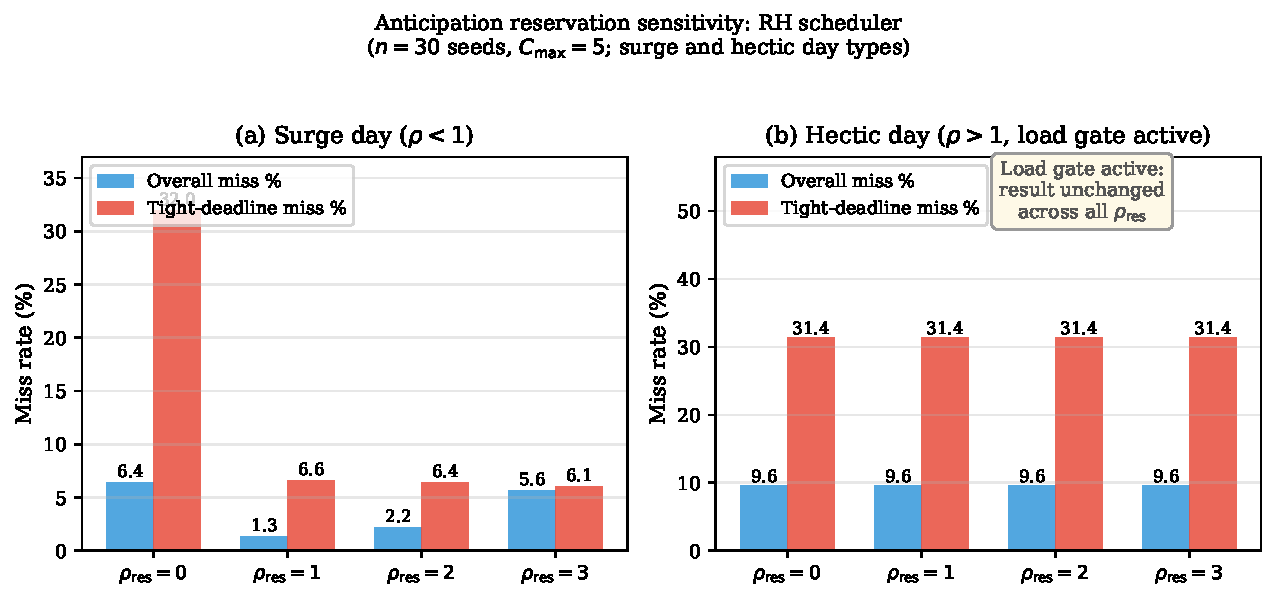
\includegraphics[width=0.98\linewidth,height=0.72\textheight,keepaspectratio]{figures/reservation_sensitivity.pdf}
\caption[Anticipation reservation sensitivity]{Anticipation reservation sensitivity for the RH scheduler: overall miss rate and tight-deadline miss rate for $\rho_{\mathrm{res}} \in \{0,1,2,3\}$ on the surge day (a, $\rho<1$) and the hectic day (b, $\rho>1$). On the surge day, a single reserved slot ($\rho_{\mathrm{res}}=1$) cuts tight-deadline miss from \ResSurgeOffTight\% to \ResSurgeOnTight\% at the cost of a modest wait increase. Reserving more slots ($\rho_{\mathrm{res}}=2,3$) offers diminishing returns and begins to push loose jobs into misses. On the hectic day, the load gate activates and all four $\rho_{\mathrm{res}}$ values produce identical results: reservation is disabled under saturation.}
\label{fig:reservation-sensitivity}
\end{figure}
\end{landscape}

\textbf{Reservation findings:} below saturation, anticipation yields a measurable benefit. On the surge day a single reserved slot ($\rho_{\mathrm{res}}=1$) cuts overall miss from \ResSurgeOffMiss\% to \ResSurgeOnMiss\% and tight-deadline miss from \ResSurgeOffTight\% to \ResSurgeOnTight\%, while loose-deadline miss stays negligible (\ResSurgeOnLoose\%): the eight-hour loose jobs have ample slack to absorb the brief idling, so their deadlines are unaffected, whereas the one-hour rush jobs that would otherwise be caught behind a burst now find a slot waiting. The cost is a modest rise in mean wait (\ResSurgeOffWait{} to \ResSurgeOnWait~min) from the deliberately idled capacity. Reserving more slots ($\rho_{\mathrm{res}}=2,3$) lowers tight miss slightly further but raises wait and begins to push loose jobs into misses, so a single reserved slot is the balanced operating point. On the hectic day every $\rho_{\mathrm{res}}$ produces the identical no-reservation result (\ResHecticGateMiss\% miss): the offered-load gate detects saturation and disables reservation, because withholding a slot from an already-saturated queue would only delay work that cannot be deferred. This load gating is why RH uses $\rho_{\mathrm{res}}=1$ throughout the study without disturbing the saturated-load headline results, which are produced with reservation gated off.


\subsection{Availability-Model Sensitivity}
\label{ssec:availability-model-sensitivity}

The per-type baseline high-stock probabilities $\beta_g$ are modelling assumptions for the on-demand pool (Section~\ref{ssec:platform-and-data}), so their influence on the scheduler comparison is tested directly: all four $\beta_g$ values are scaled by a common factor in $\{0.25, 0.50, 0.75, 1.00, 1.25\}$ and the hectic-day benchmark is re-run (30 seeds, six schedulers). Table~\ref{tab:beta_sensitivity} reports the outcome.

\begin{table}[htbp]
\centering
\caption[Availability-model sensitivity]{Availability-model ($\beta_g$) sensitivity on the hectic day ($C_{\max}=5$, 30 seeds). All four baseline high-stock probabilities are scaled by the factor in the first column; the baseline model is $\times 1.00$. Effective miss counts a job unfinished at the end of the 24-hour window as missed (every deadline in the instance falls before the window end), so the metric is immune to completion censoring at the extreme scales; the wait column, by contrast, is conditional on completion, which is why it is non-monotone across the two inoperable rows.}
\label{tab:beta_sensitivity}
\footnotesize
\setlength{\tabcolsep}{4pt}
\begin{tabular}{lrrrrrr}
\toprule
& \multicolumn{6}{c}{\textbf{Avg Wait (min) / Effective Miss \%}} \\
\cmidrule(lr){2-7}
\textbf{$\beta_g$ scale} & \textbf{FIFO} & \textbf{SPT} & \textbf{EDF} & \textbf{SPT+Rescue} & \textbf{RH} & \textbf{CADR} \\
\midrule
$\times0.25$ & 742.0\,/\,95.5 & 711.5\,/\,99.0 & 689.4\,/\,99.0 & 696.2\,/\,99.1 & 708.6\,/\,95.8 & 711.1\,/\,96.2 \\
$\times0.50$ & 906.8\,/\,91.3 & 894.1\,/\,93.3 & 907.2\,/\,97.3 & 905.6\,/\,97.5 & 900.1\,/\,89.6 & 903.2\,/\,91.6 \\
$\times0.75$ & 373.9\,/\,57.0 & 344.8\,/\,50.6 & 376.5\,/\,50.8 & 359.9\,/\,49.2 & 350.4\,/\,44.3 & 359.0\,/\,48.4 \\
$\times1.00$ \textbf{(baseline)} & 167.9\,/\,24.4 & 141.4\,/\,19.0 & 170.2\,/\,14.7 & 146.3\,/\,13.6 & 141.7\,/\,9.6 & 144.7\,/\,9.7 \\
$\times1.25$ & 87.5\,/\,12.3 & 75.6\,/\,6.4 & 86.8\,/\,0.0 & 76.7\,/\,0.0 & 75.4\,/\,5.4 & 76.9\,/\,0.0 \\
\bottomrule
\end{tabular}

\normalsize
\end{table}

Three regimes emerge, and the baseline row reproduces the Phase~3 means exactly, an incidental cross-check of the pipeline's determinism. First, availability is a first-order \emph{system} factor: at $\times 0.75$ every policy degrades steeply (effective miss \BetaThreeQuarterMinEffMiss\% to \BetaThreeQuarterMaxEffMiss\% across the full ten-policy grid, the upper end held by the deadline-blind LCF rather than by any policy in the table), and at $\times 0.50$ and below the Low state's 600 to 7{,}200\,s delays overwhelm the fleet outright: only \BetaHalfCompletedPct\% ($\times 0.50$) and \BetaQuarterCompletedPct\% ($\times 0.25$) of jobs finish within the day, and no policy, deadline-aware or not, gets its effective miss below \BetaHalfMinEffMiss\%. Second, and central to this thesis, the \emph{scheduler comparison} is stable on the scarcity side of the operable range: at $\times 0.75$ as at baseline, RH is lowest (\BetaThreeQRHmiss\%), CADR second (\BetaThreeQCADRmiss\%, closely followed by SPT+Rescue at \BetaThreeQRescueMiss\%), and the deadline-blind policies worst, so on the scarcity side the conclusions about scheduler ordering do not hinge on the exact calibration point. The ordering is statistically firm: paired $t$-tests on the published per-seed arrays at $\times 0.75$ give RH vs CADR $t=\BetaRHvCADRt$ ($\BetaRHvCADRp$) and RH vs SPT+Rescue $t=\BetaRHvRescueT$ ($\BetaRHvRescueP$). Third, at $\times 1.25$ the deadline problem becomes easy and the differences compress: CADR, EDF, and SPT+Rescue reach zero misses while RH retains a small residual (\BetaUpRHmiss\%, comparable to SPT's \BetaUpSPTmiss\%), so the RH advantage is a property of the baseline scarcity-and-saturation regime rather than a universal ordering. In summary, $\beta_g$ sets the system's overall difficulty, as expected for a per-dispatch delay term shared by all policies, while the relative merits of the schedulers, the object of this chapter, are stable across the scarcity side of the operable range ($\times 0.75$ to $\times 1.00$); on the eased side ($\times 1.25$), and under the data-ordered permutation below, the separation between deadline-aware and deadline-blind policies persists but RH yields the lead to CADR and SPT+Rescue. The sweep is reproducible via \texttt{CGRSP/phase3\_beta\_sensitivity.py}.

The remaining four policies (LCF, Balanced, Random, and the Adaptive hybrid) were also swept across all five scales (the full ten-policy grid is in the repository JSON): each tracks its Phase~3 cluster position at every operable scale, with the deadline-blind trio staying at the FIFO end and Adaptive staying adjacent to SPT+Rescue (swapping places with it at $\times 0.75$) and behind both proposed schedulers wherever the deadline problem is not already solved outright, so restricting the table to six policies discards no ordering information. Because a common scale factor perturbs the \emph{level} of the availability assumption but preserves its cross-type \emph{ranking}, two further checks target the ranking itself (both reproducible via \texttt{CGRSP/phase3\_prior\_robustness.py}). First, a data-ordered permutation: the four $\beta_g$ values are permuted so the RTX~3090 becomes the best-stocked type (0.75) and the RTX~A4000 the worst (0.50), which inverts the baseline ranking that the fixed per-type reliability priors in RH and Adaptive encode. This permutation is not a contrived stress case: it is the order in which the snapshot record ranks the four fleet types by the share of snapshots carrying any Secure Cloud offer (RTX~3090 94\%, RTX~A5000 86\%, RTX~A4500 72\%, RTX~A4000 63\%). That share measures whether a single-GPU listing is present rather than the probability that a request is fulfilled promptly, so it does not calibrate $\beta_g$, but it is the only per-type ranking the record offers, and it supports this permutation rather than the baseline ranking. Because the doubly-represented RTX~3090 inherits the highest availability, the fleet-weighted operating point becomes easier, and every policy improves: FIFO falls to \RevFIFOmiss\%, SPT to \RevSPTmiss\%, and the compressed easy-regime pattern of the $\times 1.25$ row reappears, with CADR (\RevCADRmiss\%) and SPT+Rescue (\RevRescueMiss\%) lowest, EDF (\RevEDFmiss\%) also ahead of RH, and RH at \RevRHmiss\% (significantly above CADR here, paired $t=\RevRHvCADRt$, $\RevRHvCADRp$). The deadline-blind anchor remains worst, one of the two proposed schedulers leads, and RH's own miss falls by roughly a third relative to its baseline, so the inverted prior degrades nothing catastrophically. The RH-versus-CADR order, however, does not survive: under the only per-type ranking the record supports, CADR leads and RH is significantly worse, so RH's miss lead over CADR at baseline is conditional on the assumed per-type scarcity ranking rather than robust to it, and that ranking is itself an assumption. Second, a direct ablation isolates the prior: RH re-run with the per-type reliability prior zeroed (stock-status penalty retained) on the baseline model gives \NoPriorRHmiss\% miss at \NoPriorRHwait~min wait, without a significant paired miss-rate difference from baseline RH (stock minus no-prior paired difference $\NoPriorDiffPp$ percentage points, $t=\NoPriorT$, $\NoPriorP$): this sample does not resolve a miss-rate effect from the fixed per-type prior, and does not establish that the prior is inert or that ordering alone explains RH's advantage. A third check in the same script targets the assumed arrival rate rather than $\beta_g$ (30 seeds; Section~\ref{ssec:anticipative-rolling-horizon-scheduler}): on the hectic day, assuming $0.5\times$ or $0.6\times$ the true rate (both below the gate's switching point of $\lambda\approx\PriorGateLambda$~jobs/s) lifts RH's miss from \RHMiss\% to \PriorHecUnderMiss\% and its wait from \RHWait{} to \PriorHecUnderWait~min, above FIFO's \FIFOwait~min, while every assumed rate from $0.75\times$ to $4\times$ reproduces the gated result exactly. On the surge day a $2\times$ over-estimate is inert and a $4\times$ one raises miss from \ResSurgeOnMiss\% to \ResSurgeOffMiss\%.

\subsection{Uncertainty in Estimated Execution Times}
\label{ssec:uncertainty-in-estimated-execution-times}

Three service-time cells have fewer than five observations and use estimated means and pooled log-space dispersion (Section~\ref{ssec:platform-and-data}). Their historical sample sizes do not measure their exposure in the synthetic workload: across six focal policies, these cells receive \SparseExposureLo\% to \SparseExposureHi\% of dispatches in the ten-seed baseline. Their uncertainty therefore warrants a direct check.

Table~\ref{tab:sparse_sensitivity} varies only those three cells: their means are scaled by $\times 0.75$ or $\times 1.25$, or their log-space dispersions by $\times 0.5$ or $\times 2$, while the dense cells, pricing and availability model are held fixed. These factors are modelling stress brackets, not confidence bounds estimated from the absent or sparse observations. Each arm runs the same ten seeds for FIFO, SPT, EDF, SPT+Rescue, RH and CADR; the baseline reproduces the first ten Phase~3 seeds, so it differs from the 30-seed headline. The load gate is recomputed from each arm's service model.

\begin{table}[htbp]
\centering
\caption[Estimated execution-cell sensitivity]{Deadline miss rate (\%) under estimated-cell mean and dispersion perturbations, hectic day, $C_{\max}=5$, ten paired seeds. Only the three cells with fewer than five observations are perturbed.}
\label{tab:sparse_sensitivity}
\small
\begin{tabular}{lrrrrrr}
\toprule
Estimated-cell arm & FIFO & SPT & EDF & SPT+Rescue & RH & CADR \\
\midrule
Baseline & 23.67 & 17.65 & 12.68 & 13.47 & 8.46 & 9.28 \\
Mean $\times 0.75$ & 20.76 & 12.16 & 8.40 & 6.17 & 7.07 & 5.17 \\
Mean $\times 1.25$ & 26.87 & 20.58 & 16.66 & 15.14 & 10.44 & 10.80 \\
$\sigma_{\ln}\times 0.5$ & 23.73 & 17.09 & 13.73 & 12.19 & 9.56 & 10.05 \\
$\sigma_{\ln}\times 2$ & 24.19 & 18.27 & 12.63 & 10.11 & 8.86 & 7.71 \\
\bottomrule
\end{tabular}

\end{table}

The numerical miss rates depend on these estimates. With lower estimated means, CADR has a lower point estimate than RH (\SparseMeanLowCADRMiss\% versus \SparseMeanLowRHMiss\%); with higher estimated means, RH has the lower point estimate (\SparseMeanHighRHMiss\% versus \SparseMeanHighCADRMiss\%). Neither mean perturbation separates the pair on an uncorrected paired test at 0.05. Halving the estimated-cell dispersion keeps RH ahead (\SparseSigmaLowRHMiss\% versus CADR's \SparseSigmaLowCADRMiss\%), whereas doubling it gives CADR the lower point estimate (\SparseSigmaHighCADRMiss\% versus RH's \SparseSigmaHighRHMiss\%); the raw paired $p=\SparseSigmaHighP$ for the doubled arm is not significant even before correction. The leading pair remains below the deadline-blind FIFO anchor in each tested arm, but the relative ordering and absolute miss rates should not be treated as insensitive to sparse calibration. The experiment is reproducible via \texttt{CGRSP/phase3\_sparse\_sensitivity.py}.

\subsection{Label Noise and GPU Speed Assumptions}
\label{ssec:label-noise-and-gpu-speed-assumptions}

Two assumptions in the calibration cannot be ruled out by the data and were previously only disclosed, not tested. First, the complexity class $\kappa$ is an ex-post render-time tercile that the model treats as known at arrival (Section~\ref{ssec:platform-and-data}); a deployed classifier would be imperfect. Second, the A4000 stratum means are not scene-matched: after the concurrency exclusion only two scenes are rendered on both the A4000 and the A5000, and on them its geometric-mean render time is 1.165 times the A5000's (an indicative value from very few scenes), while its pooled $\kappa=3$ stratum mean is 4\% above the A5000's (98.6\,s against 94.5\,s).

Table~\ref{tab:kappa_speed_sensitivity} brackets both on the hectic day ($C_{\max}=5$, ten seeds; the Baseline row is the ten-seed hectic-day result, as in Table~\ref{tab:sparse_sensitivity}, not the 30-seed Phase~3 figure). In the label arms the schedulers plan with an observed class that differs from the realised one; execution times, and therefore completion times and costs, always use the true class. ``Label error'' moves a job to an adjacent class with the stated probability (Low and High move to Medium, Medium moves to Low or High with equal probability); ``uninformative'' draws the observed class from the class mix independently of the job. In the speed arm every A4000 cell is scaled so that $\overline{W}(3,\text{A4000})=1.165\,\overline{W}(3,\text{A5000})$. These are stress brackets, not estimates: no classifier accuracy or corrected speed has been measured.

\begin{table}[htbp]
\centering
\caption[Complexity-label and A4000 speed sensitivity]{Deadline miss rate (\%) under complexity-label noise and a scene-matched A4000 speed, hectic day, $C_{\max}=5$, ten paired seeds. FIFO ignores the label.}
\label{tab:kappa_speed_sensitivity}
\small
\begin{tabular}{lrrrrrr}
\toprule
Arm & FIFO & SPT & EDF & SPT+Rescue & RH & CADR \\
\midrule
Baseline & 23.67 & 17.65 & 12.68 & 13.47 & 8.46 & 9.28 \\
Label error 20\% & 23.67 & 19.55 & 14.19 & 13.55 & 9.65 & 10.02 \\
Label error 40\% & 23.67 & 20.66 & 13.67 & 15.52 & 10.51 & 11.82 \\
Uninformative label & 23.67 & 23.96 & 13.07 & 18.22 & 13.02 & 14.24 \\
A4000 $\times 1.165$ & 25.92 & 20.76 & 16.76 & 14.56 & 9.28 & 11.25 \\
\bottomrule
\end{tabular}

\end{table}

RH has the lowest miss point estimate in every arm and stays below FIFO, and CADR is second in every arm except the uninformative one, where EDF (\KsUninfEDFMiss\%) is second (point estimates only: only the RH-versus-CADR pair is tested, so their separation from EDF and SPT+Rescue is not). Both have a higher miss point estimate in every degraded-label arm than at baseline (the rise reaches a raw paired-test $p<0.05$ only under the uninformative label, for RH, CADR, SPT and SPT+Rescue, and at 40\% label error for SPT and SPT+Rescue, and the rises are not monotone in the noise level; EDF, which uses the label only for node choice, also rises but not significantly in any label arm): with an uninformative label RH rises from \KsBaseRHMiss\% to \KsUninfRHMiss\% and CADR from \KsBaseCADRMiss\% to \KsUninfCADRMiss\%, leaving RH level with EDF and CADR about one point above it. The label matters most to the policies that rank jobs by estimated duration: SPT's point estimate (\KsUninfSPTMiss\%) is then above FIFO's (\KsUninfFIFOMiss\%), so its advantage over FIFO depends on the class being informative. RH has the lower point estimate than CADR in every arm, but only the scene-matched A4000 arm separates the pair on an uncorrected paired test at 0.05 (raw $p=\KsSlowRHvCADRp$, RH lower), and that arm rests on a ratio measured on only two scenes. The scene-matched A4000 raises every policy's miss rate (FIFO \KsSlowFIFOMiss\%, RH \KsSlowRHMiss\%, CADR \KsSlowCADRMiss\%; the rise is significant at raw 0.05 for FIFO, SPT and EDF) because scaling every A4000 cell by about 1.12 cuts the fleet's effective capacity at a load that already saturates it; no separate mechanism arm was run. The top of the ranking therefore holds at the level of point estimates, but the absolute miss rates in the main results are conditional on an oracle label and on the pooled A4000 mean. The experiment is reproducible via \texttt{CGRSP/phase3\_kappa\_speed\_sensitivity.py}.

\subsection{Objective-Weight Sensitivity}
\label{ssec:objective-weight-sensitivity}

The primary objective (Section~\ref{sec:mathematical-model}) is lexicographic: quality of service first, operational cost only as a tiebreaker among QoS-equivalent options. This section stress-tests that modelling choice by instead re-scoring the six focal schedulers under a fully symmetric weighted-sum scalarisation that treats QoS and cost as co-equal, $w_{\text{qos}}\, C_{\text{QoS}} + w_{\text{cost}}\, C_{\text{Cost}}$, across a grid of weights. The purpose is to show what the lexicographic priority deliberately avoids: that a symmetric scalar can be swayed by a cost difference that is near-noise at this fleet scale. Eight of the ten schedulers apply a fixed structural rule (shortest-job-first, earliest-deadline-first, laxity rescue, queue-pressure tiering, and so on) that never references the swept weights, so their decomposed metrics (wait, miss, cost) are \emph{by construction} independent of the weight choice. The Rolling-Horizon and CADR schedulers do reference cost during dispatch, but only as a minor term subordinate to the QoS penalty (RH) or as a tiebreaker among deadline-feasible nodes (CADR), and their decisions are held at that fixed configuration rather than re-optimised at each grid point.

For each of six focal schedulers (FIFO, SPT, EDF, SPT+Rescue, RH and CADR), per-seed waiting time, deadline-miss rate, and operational cost are collected on the hectic-day workload ($n=10$ seeds) and the composite objective is then evaluated post-hoc across a grid of weights. The mean per-job QoS penalty is $\alpha_1(60\,\overline{w}_{\rm min}) + \alpha_2(\Delta_{\rm miss,\%}/100)$, so wait is converted to seconds and miss percentage to a fraction before weighting. Thus $\alpha_2/\alpha_1=10$ equates one missed job with ten seconds of waiting, not with ten minutes or ten percentage points. Because the raw QoS component (seconds) and cost component (US dollars) lie on very different scales, each component is min-max normalised across the six focal schedulers before the weights are applied, so that $w_{\text{cost}}$ has a genuine effect on the ranking (a raw weighted sum would be entirely QoS-dominated). Table~\ref{tab:weight_sensitivity} reports two sweeps: the multi-objective weight $w_{\text{cost}} \in \{0.1, 0.3, 0.5, 0.7, 0.9\}$ (with the QoS ratio fixed at the baseline $\alpha_2/\alpha_1 = 10$), and the deadline-penalty ratio $\alpha_2/\alpha_1 \in \{1, 5, 10, 20, 50\}$ (with $w_{\text{qos}} = w_{\text{cost}} = 0.5$); Figure~\ref{fig:weight-sensitivity} plots the deadline-penalty sweep for both the miss-indicator and the tardiness objective.

\begin{table}[htbp]
\centering
\caption[Objective-weight sensitivity]{Objective-weight sensitivity: normalised composite objective per scheduler (lower is better) on the hectic day ($n=10$ seeds, $C_{\max}=5$). Components are min-max normalised across schedulers before weighting. The minimum (winning) scheduler in each row is \textbf{bold}; the symmetric reference configuration ($w_{\text{qos}}=w_{\text{cost}}=0.5$, $\alpha_2/\alpha_1=10$) appears as the marked row in both panels.}
\label{tab:weight_sensitivity}
\begin{tabular}{lrrrrrr}
\toprule
& \multicolumn{6}{c}{\textbf{Composite objective (normalised, lower is better)}} \\
\cmidrule(lr){2-7}
\textbf{Weight setting} & \textbf{FIFO} & \textbf{SPT} & \textbf{EDF} & \textbf{SPT+Rescue} & \textbf{RH} & \textbf{CADR} \\
\midrule
$w_{\text{cost}}=0.1$ & 0.92 & \textbf{0.04} & 0.99 & 0.21 & 0.12 & 0.22 \\
$w_{\text{cost}}=0.3$ & 0.94 & \textbf{0.11} & 0.98 & 0.16 & 0.24 & 0.34 \\
$w_{\text{cost}}=0.5$ \textbf{(baseline)} & 0.96 & 0.18 & 0.96 & \textbf{0.12} & 0.36 & 0.45 \\
$w_{\text{cost}}=0.7$ & 0.97 & 0.25 & 0.95 & \textbf{0.07} & 0.48 & 0.57 \\
$w_{\text{cost}}=0.9$ & 0.99 & 0.32 & 0.93 & \textbf{0.02} & 0.61 & 0.68 \\
\midrule
$\alpha_2/\alpha_1=1$ & 0.96 & 0.18 & 0.96 & \textbf{0.12} & 0.36 & 0.45 \\
$\alpha_2/\alpha_1=5$ & 0.96 & 0.18 & 0.96 & \textbf{0.12} & 0.36 & 0.45 \\
$\alpha_2/\alpha_1=10$ \textbf{(baseline)} & 0.96 & 0.18 & 0.96 & \textbf{0.12} & 0.36 & 0.45 \\
$\alpha_2/\alpha_1=20$ & 0.96 & 0.18 & 0.96 & \textbf{0.11} & 0.36 & 0.45 \\
$\alpha_2/\alpha_1=50$ & 0.96 & 0.18 & 0.96 & \textbf{0.11} & 0.36 & 0.45 \\
\bottomrule
\end{tabular}

\end{table}

No scheduler wins every weighting on this grid. SPT wins at the two lowest cost weights ($w_{\text{cost}}=0.1$ and $0.3$), where the wait term dominates the composite, and SPT+Rescue wins from $w_{\text{cost}}=0.5$ upward and at every deadline-penalty ratio; RH never wins, placing second at $w_{\text{cost}}=0.1$ and third elsewhere, and CADR is fourth throughout. The ranking is decided by cost, not by QoS: on these ten seeds SPT+Rescue is the cheapest policy (\$6.34 against \$6.37 for RH, \$6.38 for CADR and \$6.39 for FIFO and EDF, a spread of 0.9\%), and min-max normalisation stretches that sub-one-percent spread over the whole 0 to 1 scale, so once $w_{\text{cost}}$ reaches 0.5 a cost gap of a few cents outweighs RH's lowest miss rate. EDF and FIFO have the highest composites throughout because they have the highest mean waits. The 30-seed Phase~3 cost ranking differs (SPT is cheapest there), so this ordering is itself a ten-seed point estimate.

Under the symmetric scalar, the winner changes with the cost weight and is decided by a cost difference of under one percent that lies within seed noise, so the scalarisation fragility that motivates a lexicographic rather than a symmetric objective is demonstrated here directly: a symmetric scalar can place a policy that misses substantially more deadlines (SPT+Rescue) above the miss leader (RH) because of a few cents of rental cost. The thesis therefore adopts the lexicographic form (Section~\ref{sec:mathematical-model}) as the principled choice, since the lexicographic priority rules such a reordering out by construction rather than leaving it to the weights.

The decomposed conclusions are unaffected. RH holds the lowest miss point estimate among the focal schedulers irrespective of the weights (the 30-seed Phase~3 means are \RHMiss\% and \RHWait~min; the ten-seed subset used here gives slightly lower values), and the composite win of SPT+Rescue on this grid does not contradict those decomposed metrics; it reflects the cost axis alone. This is why the primary comparisons in this thesis report wait, miss, and cost separately (Section~\ref{sec:mathematical-model}) rather than collapsing them into a single weighted score. Operational cost headroom is structurally small across all policies, and CADR's cost-aware node selection does not make it the cheapest policy overall; the cost differences across all schedulers are near-noise at this scale, which is exactly why they can decide a min-max normalised composite.

\textbf{Tardiness-objective robustness.} As an additional check, each scheduler is re-scored post-hoc against a tardiness-based objective (replacing the dimensionless binary miss indicator $1-\delta_j$ with continuous tardiness $\tau_j$ measured in seconds) on the same hectic-day workload ($n=10$ seeds). The same numerical $\alpha_2/\alpha_1$ grid is reused, but its units change: in the binary score the ratio is seconds of waiting per missed job, whereas in the tardiness score it is seconds of waiting per second of lateness. Thus the change in winner reflects both the penalty form and its effective scale, not a controlled comparison at equal economic penalty per breach. Table~\ref{tab:tardiness_objective} reports the resulting composite scores.

\begin{table}[htbp]
\centering
\caption[Tardiness-objective re-scoring]{Tardiness-objective re-scoring: normalised composite score with a tardiness term (lower is better) by deadline-penalty ratio, hectic day ($n=10$ seeds, $C_{\max}=5$). Compare with the miss-indicator objective in Table~\ref{tab:weight_sensitivity}.}
\label{tab:tardiness_objective}
{\small\begin{tabular}{lrrrrrr}
\toprule
& \multicolumn{6}{c}{\textbf{Composite with tardiness term (normalised, lower is better)}} \\
\cmidrule(lr){2-7}
\textbf{$\alpha_2/\alpha_1$} & \textbf{FIFO} & \textbf{SPT} & \textbf{EDF} & \textbf{SPT+Rescue} & \textbf{RH} & \textbf{CADR} \\
\midrule
$\alpha_2/\alpha_1=1$ & 1.00 & 0.18 & 0.75 & \textbf{0.03} & 0.59 & 0.37 \\
$\alpha_2/\alpha_1=5$ & 0.98 & 0.26 & 0.54 & \textbf{0.02} & 0.83 & 0.37 \\
$\alpha_2/\alpha_1=10$ & 0.93 & 0.27 & 0.49 & \textbf{0.01} & 0.83 & 0.37 \\
$\alpha_2/\alpha_1=20$ & 0.91 & 0.28 & 0.47 & \textbf{0.01} & 0.83 & 0.37 \\
$\alpha_2/\alpha_1=50$ & 0.89 & 0.29 & 0.46 & \textbf{0.02} & 0.83 & 0.38 \\
\bottomrule
\end{tabular}
}
\end{table}

\begin{landscape}
\begin{figure}[H]
\centering
\captionsetup{font=small,skip=6pt}
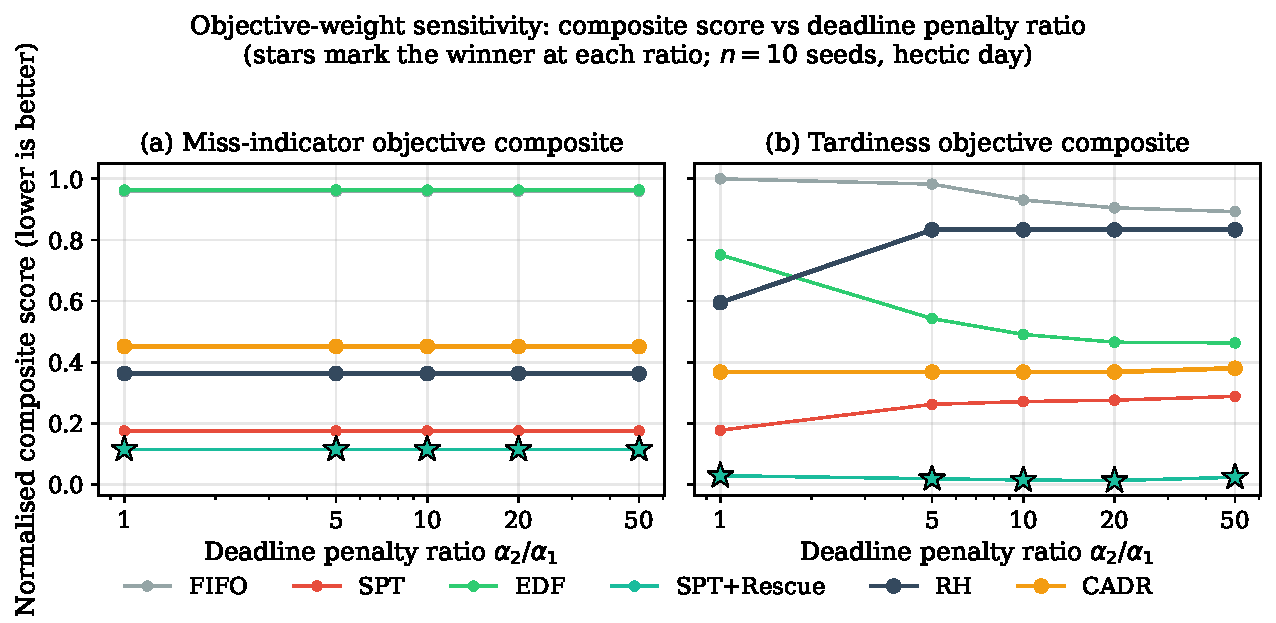
\includegraphics[width=0.98\linewidth,height=0.72\textheight,keepaspectratio]{figures/weight_sensitivity.pdf}
\caption[Objective-weight sensitivity]{Objective-weight sensitivity: normalised composite score (lower is better) versus the deadline-penalty ratio $\alpha_2/\alpha_1$ at the symmetric weighting $w_{\text{qos}}=w_{\text{cost}}=0.5$. Stars mark the winner at each ratio. Panel~(a), miss-indicator objective: SPT+Rescue wins at every ratio, reflecting its lowest cost on these ten seeds and a wait close to SPT's; the panel is essentially flat in the ratio (every composite moves by under 0.002 between $\alpha_2/\alpha_1=1$ and $50$) because the scaled wait term dominates the QoS score, so it tests the winner, not sensitivity to the ratio. Panel~(b), tardiness objective: SPT+Rescue also wins at every ratio; RH's score starts lower (third of the six at $\alpha_2/\alpha_1=1$) but rises sharply as the ratio grows, plateauing at a mid-pack value by $\alpha_2/\alpha_1=10$, because tight jobs it promotes too late fall into its demoted tier and carry high tardiness that is increasingly penalised as the ratio grows; EDF's score falls as the ratio grows since its low tardiness is increasingly rewarded, though it remains behind SPT+Rescue, SPT and CADR. The scalarised winner is the same in both scores here, while the per-metric leaders (Table~\ref{tab:statistical}) are different policies.}
\label{fig:weight-sensitivity}
\end{figure}
\end{landscape}

The tardiness composite is also won by SPT+Rescue at every penalty ratio (Table~\ref{tab:tardiness_objective}), followed by SPT and then CADR: SPT+Rescue combines the lowest cost on these ten seeds with a wait close to SPT's and a low mean tardiness, while CADR's lower tardiness is outweighed by its slightly higher wait and cost. RH, the miss-count leader on point estimate, drops to a lower-mid score here and does not improve as the tardiness weight $\alpha_2/\alpha_1$ rises, because RH's late promotion of tight jobs, which then fall into its demoted tier, gives it the highest mean tardiness of the six schedulers compared here (Random's tardiness is higher still in the full ten-scheduler comparison of Section~\ref{sec:phase-3-statistical-validation}); EDF's score falls as that weight grows, since its low tardiness is increasingly rewarded, though it remains behind SPT+Rescue, SPT and CADR throughout. This does not indicate a robustness failure; it sharpens the central distinction of the thesis: RH minimises the \emph{count} of missed deadlines, not their severity, so it does not lead a tardiness-weighted objective under any ratio tested. The per-metric leaders are RH for miss count and, among the two proposed schedulers, CADR for tardiness (Adaptive, EDF and SPT+Rescue post comparably low tardiness but do not match RH or CADR on miss); the single scalarised winner is a third policy, SPT+Rescue, whose edge comes from cost and wait, and the rescoring cannot attribute any change in winner solely to the penalty form, since its units and effective scale also differ. The practical reading is therefore objective-dependent by design: an operator who penalises lateness continuously should use CADR rather than RH, and since the paired baseline binary-miss test does not resolve the difference between them, CADR is also the default for an operator who penalises misses as binary events, with RH kept as the specialist for the scarce baseline regime, where its miss point estimate is lowest (Section~\ref{sec:mathematical-model}).

\subsection{Fleet-Composition Sensitivity}
\label{ssec:fleet-composition-sensitivity}

The headline fleet is fixed at two RTX~3090 slots and one each of the RTX~A5000, A4500 and A4000. Table~\ref{tab:fleet_mix} reports the mean miss rate for the six mixes. To test whether the policy ordering depends on that composition, six five-slot mixes are run for ten seeds (0 to 9) each: the all-types anchor, three mixes in which one type occupies three slots, and two single-type fleets. The anchor reproduces the first ten seeds of the Phase~3 record in \texttt{statistical.json} exactly (360 of 360 compared values across six policies and six metrics), so it is the same workload and dispatch path as the headline experiment. The other mixes keep the job stream and the policy implementations, but a different fleet changes which slot is free at each dispatch, so their service draws need not match the anchor seed by seed. The sweep is a sensitivity check at $n=10$, not a second workload, and it is not a second studio trace.

\begin{table}[htbp]
\centering
\caption[Fleet-composition sensitivity]{Fleet-composition sensitivity: mean deadline miss rate (\%) for six five-slot mixes, ten seeds each, on the Phase~3 hectic day ($\sim$950 jobs/day, $C_{\max}=5$, $\lambda=0.100$ j/s, 20\% tight 1h / 80\% loose 8h deadlines). The Slots column gives the slot counts in the order RTX~3090 / RTX~A5000 / RTX~A4500 / RTX~A4000. Bold marks the lowest miss rate in each row. The all-types row reproduces the first ten Phase~3 seeds; the other rows are sensitivity checks at $n=10$, not separate headline tests.}
\label{tab:fleet_mix}
\small
\begin{tabular}{llrrrrrr}
\toprule
\textbf{Mix} & \textbf{Slots} & \textbf{FIFO} & \textbf{SPT} & \textbf{EDF} & \textbf{SPT+Rescue} & \textbf{RH} & \textbf{CADR} \\
\midrule
All-types & 2/1/1/1 & 23.67 & 17.65 & 12.68 & 13.47 & \textbf{8.46} & 9.28 \\
3090-heavy & 3/1/0/1 & 28.51 & 22.01 & 18.14 & 17.37 & \textbf{12.94} & 13.46 \\
A5000-heavy & 1/3/0/1 & 23.60 & 16.77 & 12.79 & 9.13 & 9.27 & \textbf{8.15} \\
A4000-heavy & 1/1/0/3 & 15.79 & 7.31 & 2.07 & 1.36 & 5.96 & \textbf{0.57} \\
3090-only & 5/0/0/0 & 36.23 & 31.14 & 28.13 & 25.71 & \textbf{22.11} & 23.12 \\
A5000-only & 0/5/0/0 & 25.43 & 19.42 & 14.45 & 13.85 & \textbf{8.84} & 9.55 \\
\bottomrule
\end{tabular}

\end{table}

Two features are stable across the six mixes. First, RH and CADR are the two lowest-miss policies in the all-types, 3090-heavy, 3090-only and A5000-only mixes. Second, every deadline-aware policy (EDF, SPT+Rescue, RH and CADR) has a lower mean miss than FIFO in every mix. The ordering is not stable overall: the JSON's ordering flag is false because the A5000-heavy and A4000-heavy mixes place CADR and SPT+Rescue in the two lowest positions, with RH third and fourth respectively.

The A5000-heavy reversal is a point-estimate ordering, not a resolved one. RH and CADR differ by 1.12 percentage points (9.27\% against 8.15\%, paired $p=0.282$, pooled $d=0.287$), and RH and SPT+Rescue differ by 0.14 points ($p=0.916$, pooled $d=0.041$). Neither difference is significant, so this mix does not establish that either policy is better on miss; it shows only that RH's lead does not persist in the point estimates.

The A4000-heavy reversal is decisive. CADR's 0.57\% miss is far below RH's 5.96\% (paired $p<0.001$, pooled $d=6.21$), and SPT+Rescue (1.36\%) is also below RH (uncorrected $p=0.0038$). This is the easiest mix in the sweep for every policy, with FIFO at 15.79\% against 23.67\% in the anchor, but CADR's advantage over RH is significant and large.

Across the six mixes, RH is the lowest-miss point estimate in four and CADR in two. CADR is never more than about one percentage point above the mix minimum (its largest gap is 1.01 points in the 3090-only mix), whereas RH falls 5.39 points behind in the A4000-heavy mix. The ordering is therefore composition-dependent, and CADR is the more robust default: it is at or near the minimum in every mix and leads in the two mixes where RH's lead reverses. RH remains the lowest-miss policy in four of the six mixes, including the baseline all-types fleet; the composition dependence, not a universal RH lead, is the finding. The $n=10$ sweep is a sensitivity check, not a headline test, and the cross-mix service draws differ in dispatch order; a second studio trace remains the open generalisation test.

\section{Phase 4: Monthly Operational Simulation}
\label{sec:phase-4-monthly-operational-simulation}

Phases 2 and 3 benchmark schedulers on hectic-day workload ($\sim$950 jobs/day) and characterise performance across all day types. Phase 4 evaluates the same schedulers over a month whose day-type mix is taken from RunPod billing, with each day type's job count as in Section~\ref{ssec:platform-and-data}. Because every hectic day carries the assumed stress-load count, a simulated month holds about 7,600 jobs on average over the ten replications, roughly 60\% of them on hectic days. That is about three times the busiest month in the job record (about 2,400 jobs, September 2025). Phase~4 therefore spreads the hectic-day stress-load assumption over a billing-derived calendar rather than testing it independently.

\textbf{Results.} Table~\ref{tab:phase4} summarises monthly outcomes; Figure~\ref{fig:cost-comparison} isolates the cost dimension for both the hectic-day and the monthly horizon. Figure~\ref{fig:phase4} shows waiting time by day type and monthly deadline miss rates. Figure~\ref{fig:phase4-timeline} shows the daily miss rate trajectory over a representative 30-day replication, illustrating how performance tracks the day-type sequence: hectic and surge days produce sharp spikes while normal and quiet days remain near zero for all schedulers.

\begin{table}[htbp]
\centering
\caption[Phase 4 monthly summary]{Phase 4 monthly outcome summary per scheduler: wait, miss, tardiness, and cost ($C_{\max}=5$, 30 days, 10 replications, 20\% tight 1h / 80\% loose 8h deadlines)}
\label{tab:phase4}
\resizebox{\linewidth}{!}{\begin{tabular}{lrrrrr}
\toprule
\textbf{Scheduler} & \textbf{Avg Wait (min)} & \textbf{95\% CI} & \textbf{Miss\%} & \textbf{Avg Tardiness (min)} & \textbf{Cost (\$/mo)} \\
\midrule
\textbf{RH} & 103.73 & [95.28,~112.17] & \textbf{6.57} & 19.07 & 48.31 \\
CADR & 104.09 & [95.14,~113.03] & 7.06 & 6.27 & 48.43 \\
SPT+Rescue & 104.29 & [95.83,~112.75] & 8.96 & 5.19 & 48.67 \\
Adaptive & 116.81 & [107.85,~125.78] & 7.53 & 3.51 & 48.67 \\
\textbf{SPT} & \textbf{101.92} & [93.18,~110.66] & 12.86 & 10.69 & 48.56 \\
EDF & 116.69 & [106.50,~126.88] & 8.92 & 3.77 & 50.67 \\
LCF & 114.64 & [105.08,~124.20] & 16.50 & 17.82 & 48.52 \\
Balanced & 116.70 & [106.64,~126.77] & 16.55 & 18.26 & 49.11 \\
FIFO & 116.09 & [106.21,~125.97] & 16.74 & 18.02 & 53.08 \\
Random & 116.39 & [106.08,~126.71] & 15.62 & 22.32 & 51.48 \\
\bottomrule
\end{tabular}
}
\end{table}

\begin{landscape}
\begin{figure}[H]
\centering
\captionsetup{font=small,skip=6pt}
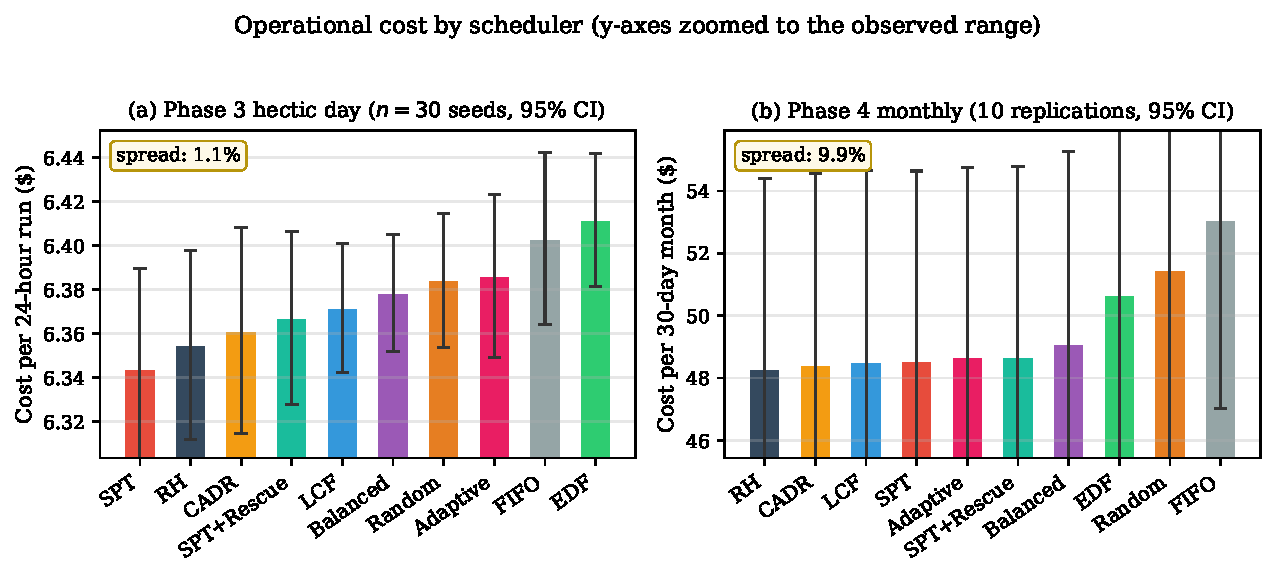
\includegraphics[width=0.98\linewidth,height=0.72\textheight,keepaspectratio]{figures/cost_comparison.pdf}
\caption[Operational cost by scheduler]{Operational cost by scheduler, with y-axes zoomed to the observed range and 95\% confidence intervals. (a)~Phase~3 hectic-day cost per 24-hour run: the spread between the cheapest and most expensive policy (SPT and EDF) is about \CostSpreadPct\%, small beside the QoS differences, and the confidence intervals of every pair of policies overlap, which is why cost cannot meaningfully discriminate between the schedulers under saturation. (b)~Phase~4 monthly cost across the full day-type mix: the spread widens (FIFO, Random, and EDF incur the highest monthly costs), but the confidence intervals still overlap heavily, and the two proposed schedulers sit at the cheap end of the range.}
\label{fig:cost-comparison}
\end{figure}
\end{landscape}

\begin{landscape}
\begin{figure}[H]
\centering
\captionsetup{font=small,skip=6pt}
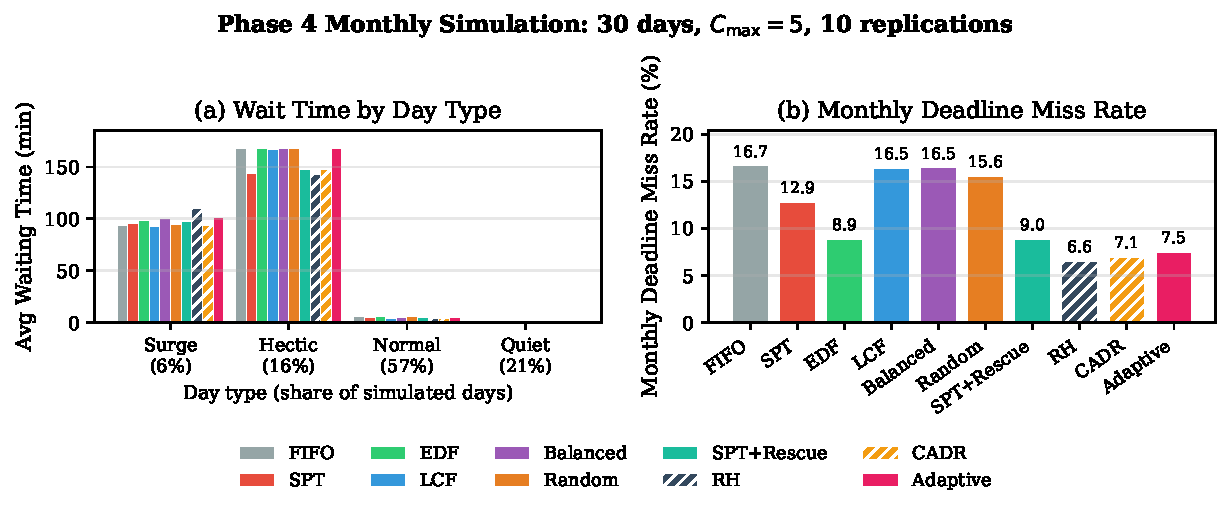
\includegraphics[width=0.98\linewidth,height=0.72\textheight,keepaspectratio]{figures/phase4_monthly.pdf}
\caption[Phase 4 monthly results]{Phase 4 monthly simulation ($C_{\max}=5$, 30 days, 10 replications, 20\% tight 1h / 80\% loose 8h). (a) Average waiting time by day type: the hectic cohorts have the largest wait, surge cohorts also show substantial queueing, and normal and quiet cohorts have much smaller waits. (b) Monthly miss rate: RH \PhFourRHMiss\% and CADR \PhFourCADRMiss\% (the lowest tier; no paired test is computed at this phase), SPT+Rescue \PhFourRescueMiss\%, SPT \PhFourSPTmiss\%; EDF \PhFourEDFmiss\%; Random \PhFourRandomMiss\%; FIFO/LCF/Balanced \PhFourFIFOmiss{} to \PhFourLCFmiss\%.}
\label{fig:phase4}
\end{figure}
\end{landscape}

\begin{landscape}
\begin{figure}[H]
\centering
\captionsetup{font=small,skip=6pt}
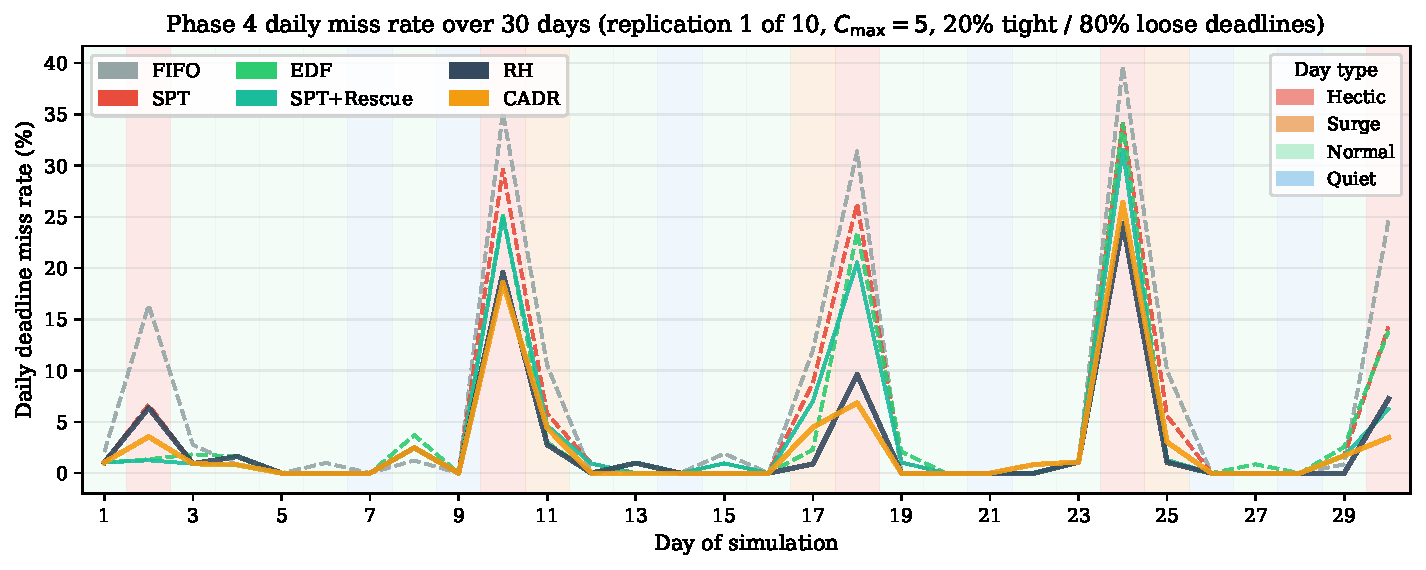
\includegraphics[width=0.98\linewidth,height=0.72\textheight,keepaspectratio]{figures/phase4_timeline.pdf}
\caption[Daily miss rate over the simulated month]{Daily deadline miss rate over 30 simulation days (replication~1 of 10, $C_{\max}=5$). Background shading indicates day type: red for hectic, orange for surge, green for normal, blue for quiet. RH (dark) and CADR (gold) are typically among the lowest spikes on hectic days, though EDF and SPT+Rescue occasionally match or beat them on individual days; FIFO (grey) provides the deadline-oblivious reference among the six policies shown. On normal and quiet days all schedulers converge near zero. The temporal structure confirms that scheduler choice is consequential only on the two heavy day types (hectic, above saturation, and surge, below saturation on execution load but with provisioning delays building a long queue), consistent with the Phase~3 day-type sensitivity analysis (Section~\ref{ssec:day-type-sensitivity-c-max-5}).}
\label{fig:phase4-timeline}
\end{figure}
\end{landscape}

On the continuous calendar RH and CADR are the two lowest-miss point estimates: RH \PhFourRHMiss\% and CADR \PhFourCADRMiss\%. RH records \PhFourRHWait~min wait and CADR \PhFourCADRwait~min, both above SPT (\PhFourSPTwait~min) and slightly below SPT+Rescue (\PhFourRescueWait~min). RH has the lower miss point estimate and CADR the lower tardiness (\PhFourCADRTard~min against \PhFourRHtard~min). No paired policy-comparison test is reported at Phase~4, so these differences describe point estimates rather than an established separation, and at $\times 1.25$ availability or under the data-ordered ranking CADR (among others) leads RH (Section~\ref{ssec:availability-model-sensitivity}). The Phase~3 paired evidence remains the basis for statements about statistical ties or superiority.

The reservation ablation measures a different question on the same ten monthly calendars and seeds. Disabling RH's anticipation lowers mean wait by \MonthResWaitDelta~min ($\MonthResWaitP$) while raising miss by \MonthResMissDelta~percentage points ($\MonthResMissP$) and mean tardiness by \MonthResTardDelta~min ($\MonthResTardP$). These are uncorrected paired tests, reported separately from the Phase~3 family. With anticipation off, RH records \MonthResOffWait~min wait and \MonthResOffMiss\% miss. The gate remains active on surge, normal and quiet days, is disabled on hectic days, and is also disabled while the final backlog drains after the calendar closes. Thus the monthly anticipation trade-off is measured under a persistent queue.

CADR's main advantage is miss severity: \PhFourCADRTard~min mean tardiness against RH's \PhFourRHtard~min. Figure~\ref{fig:tardiness_tradeoff} shows that neither proposed scheduler dominates the other on miss and tardiness: RH has the lower miss point estimate, CADR the lower tardiness. The Adaptive hybrid has the lowest monthly mean tardiness of all ten policies (\PhFourAdaptiveTard~min), below EDF's \PhFourEDFtard~min, but has higher miss (\PhFourAdaptiveMiss\%) than both proposed schedulers. CADR remains the recommended default for the combination of low miss and lower lateness, with RH preferred when the breach count is the overriding concern in the scarce baseline model; the small monthly miss difference is not presented as a tested advantage.

\begin{landscape}
\begin{figure}[H]
\centering
\captionsetup{font=small,skip=6pt}
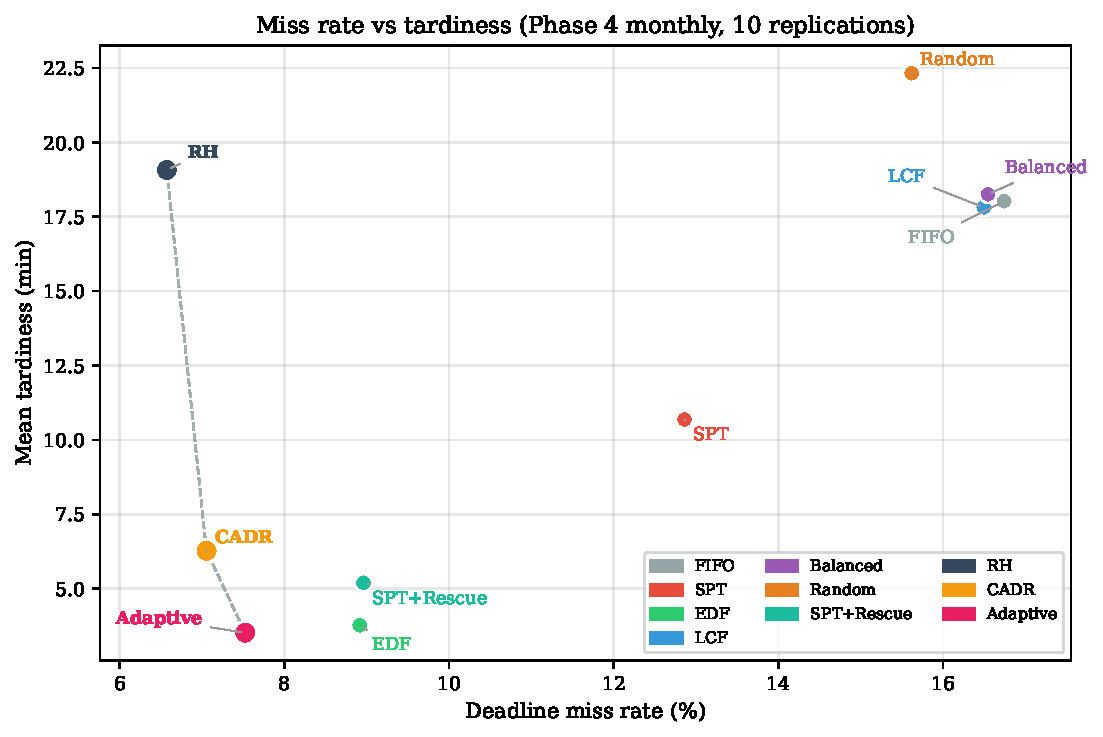
\includegraphics[width=0.98\linewidth,height=0.75\textheight,keepaspectratio]{figures/tardiness_tradeoff.pdf}
\caption[Miss rate vs tardiness trade-off]{Miss rate versus mean tardiness, continuous Phase~4 calendar ($C_{\max}=5$, ten replications). RH and CADR occupy the lowest-miss region (\PhFourRHMiss\% and \PhFourCADRMiss\%); RH has lower miss and CADR lower tardiness (\PhFourRHtard~min and \PhFourCADRTard~min). The Adaptive hybrid holds the lowest-tardiness end of the point-estimate frontier. No paired policy-comparison test is reported for this phase.}
\label{fig:tardiness_tradeoff}
\end{figure}
\end{landscape}

The Adaptive hybrid's \PhFourAdaptiveMiss\% miss improves on SPT+Rescue (\PhFourRescueMiss\%), EDF (\PhFourEDFmiss\%) and SPT (\PhFourSPTmiss\%), but RH and CADR both have lower miss and wait point estimates. EDF retains a low-tardiness profile, with \PhFourEDFmiss\% miss and \PhFourEDFwait~min wait; the Adaptive hybrid is numerically below it on miss and tardiness. Deadline-oblivious FIFO, LCF and Balanced remain substantially worse on miss, at \PhFourFIFOmiss\%, \PhFourLCFmiss\% and \PhFourBalancedMiss\% respectively. Both proposed schedulers reduce the FIFO monthly miss rate by more than half.

The hectic-day submission cohorts carry most of the missed deadlines: FIFO reaches \PhFourHecFIFOmiss\%, SPT \PhFourHecSPTmiss\%, and SPT+Rescue \PhFourHecRescueMiss\%. These cohort rates differ from the single-day Phase~3 estimates because the monthly experiment samples different job counts and seeds and retains queue and fleet state between days. The month is therefore a separate operational experiment, not a weighted average of independent daily benchmarks.

\section{Summary of Findings}
\label{sec:summary-of-findings}

Table~\ref{tab:findings} consolidates the key empirical findings from all phases.

\footnotesize
\begin{singlespace}
\begin{longtable}{>{\RaggedRight}p{0.29\textwidth} >{\RaggedRight}p{0.27\textwidth} >{\RaggedRight}p{0.33\textwidth}}
\caption{Summary of key experimental findings}\label{tab:findings}\\
\toprule
\textbf{Finding} & \textbf{Quantitative evidence} & \textbf{Practical implication} \\
\midrule
\endfirsthead
\toprule
\textbf{Finding} & \textbf{Quantitative evidence} & \textbf{Practical implication} \\
\midrule
\endhead
\bottomrule
\endfoot
SPT achieves the lowest baseline wait under capacity saturation ($\rho>1$), tied with RH; EDF achieves significantly lower miss (hectic, 20\%/80\% deadlines) & \SPTwait~min wait ($d=\SPTFIFOwaitD$ vs FIFO, $p<0.001$); \SPTmiss\% miss ($d=\SPTFIFOmissD$, $p<0.001$; EDF \EDFmiss\%, $p<0.001$), $n=30$ & SPT is the strongest low-wait baseline; the deadline-aware default is CADR, with RH the specialist for the scarce baseline regime (rows 1 and 4, Table~\ref{tab:rh_vs_cadr}) \\ \addlinespace
SPT+Rescue's laxity-rescue limits tight-deadline starvation under saturation & \RescueWait~min wait ($d=\RescueFIFOwaitD$, $p<0.001$); \RescueMiss\% miss ($d=\RescueFIFOmissD$, $p<0.001$) & Acceptable alternative when tight-deadline compliance is a strict requirement \\ \addlinespace
EDF achieves significantly lower miss than SPT; its wait is not significantly different from FIFO's & $d=\EDFFIFOmissD$ miss vs FIFO ($p<0.001$); $d=\EDFFIFOwaitD$ wait vs FIFO ($p=\EDFFIFOwaitP$, not significant) & EDF buys deadline safety with no wait advantage to show for it; prefer SPT when wait also matters \\ \addlinespace
Among the baseline policies in the sweep (surge, $\rho<1$), EDF's miss is significantly lower at $f_{\text{tight}} \leq 30\%$ and SPT's at $f_{\text{tight}} \geq 70\%$, their paired difference not significant at $f_{\text{tight}} = 50\%$ & EDF \DlTenEDFmiss\% vs SPT \DlTenSPTmiss\% at 10\% tight ($\DlTenSPTEDFmissP$); \DlFiftyEDFmiss\% vs \DlFiftySPTmiss\% at 50\% ($\DlFiftySPTEDFmissP$); SPT \DlSeventySPTmiss\% vs EDF \DlSeventyEDFmiss\% at 70\% ($\DlSeventySPTEDFmissP$) & Follow the tight-deadline-fraction boundary: EDF or SPT+Rescue for low tight fractions, SPT for high ones, either near the middle of the range \\ \addlinespace
RH achieves best-tier monthly miss (\PhFourRHMiss\%, near-identical to CADR); its monthly wait no longer leads, sitting within about two minutes of SPT's, CADR's and SPT+Rescue's & \PhFourRHMiss\% (RH) vs \PhFourFIFOmiss\% (FIFO); RH wait \PhFourRHWait~min vs SPT \PhFourSPTwait~min & At monthly scale RH and CADR have the two lowest miss point estimates (RH marginally lower, no paired test), consistent with CADR as the default; any preference for RH on miss count rests on Phase~3, and RH's wait advantage does not persist to monthly scale \\ \addlinespace
CADR achieves near-RH miss at substantially lower tardiness; matches SPT+Rescue's wait rather than beating it & Phase~3: \CADRmiss\% miss, \CADRtard~min tardiness vs RH \RHtard~min; Phase~4: \PhFourCADRMiss\% miss, \PhFourCADRTard~min tardiness vs RH \PhFourRHtard~min & Deploy CADR as the default: the Phase~3 miss difference from RH is not significant ($p=\RHCADRmissP$), but equivalence is untested; CADR has close monthly miss point estimates with lower tardiness, and leads under eased availability and the data-ordered ranking, and cuts tardiness substantially; keep RH for the scarce baseline regime when the lowest miss count is what matters (SPT where queue wait is the priority) \\ \addlinespace
\end{longtable}
\end{singlespace}
\normalsize

} % end \sloppy

\chapter{Discussion and Future Work}
\label{chap:conclusion}
{%

\section{Theoretical Implications}
\label{sec:theoretical-implications}

This thesis formalises the Cloud GPU Rendering Scheduling Problem (CGRSP) as an online bi-objective scheduling problem on heterogeneous, stochastically available GPU fleets. The gap it fills is specific: cloud GPU rental markets (RunPod, Lambda Labs, CoreWeave) expose fine-grained billing (per second on RunPod), qualitative node availability, and mixed deadline constraints that reserved-cluster schedulers do not handle, yet no prior scheduling work addresses all three simultaneously.

\textbf{Problem formulation.} Chapter~\ref{chap:formulation} develops this into notation, decision variables, and constraints for scheduling under stochastic provisioning delays. The three-state availability model (unavailable / idle / running; the unavailable state does not occur on the on-demand platform studied) captures the consumer's limited observability of cloud node state, without knowledge of the underlying provisioning dynamics, and is sufficient for practical policy construction, while the bi-objective function explicitly balances QoS (waiting time, deadline miss rate) against operational cost.

\textbf{Simulator construction.} Chapter~\ref{chap:system} describes the discrete-event simulator, calibrated against 6,234 real RunPod rendering jobs. The simulator reproduces the empirical execution-time distribution and adds two modelled components: Poisson job arrivals at day-type rates (the hectic and surge loads being stress assumptions above the busiest recorded day), and stochastic, stock-status-driven provisioning delays whose stock-status probabilities are assumed rather than measured. Execution times are sampled from per-stratum log-normal service distributions whose means equal the per-stratum means of those jobs for the nine well-sampled strata (the three sparse strata use relative-performance estimates, see the limitations below) and whose log-space dispersions are fitted from the same data. Simulation is used because live A/B testing on a production cluster is not feasible at this evaluation scale.

\textbf{Algorithm comparison.} Four experimental phases with heterogeneous deadlines (20\% tight 1h / 80\% loose 8h) support the following conclusions.

SPT achieves a lowest-tier wait under capacity saturation ($\rho>1$), with no significant paired wait difference from RH, though EDF now achieves significantly lower miss. Across $n=30$ seeds on the assumed hectic-day stress workload ($\sim$950 jobs/day, against a busiest recorded day of 415; $C_{\max}=5$), it records a lowest-tier wait (\SPTwait~min, $d=\SPTFIFOwaitD$ vs FIFO, $p<0.001$; with no significant paired wait difference from RH's \RHWait~min, $p=\RHSPTwaitP$) but a significantly higher miss rate than EDF (\SPTmiss\% vs EDF's \EDFmiss\%, $d=\SPTEDFmissD$, $p<0.001$). This finding is consistent with the classical single-machine SPT result~\cite{smith1956various} and its M/G/1 queueing counterpart~\cite{pinedo2016scheduling} in the heterogeneous multi-machine setting of this simulation: under heavy overload, shortest-job-first ordering achieves the lowest mean wait among the baseline policies, but deadline ordering alone now achieves significantly better deadline performance.
SPT+Rescue limits tight-deadline starvation at a notably lower miss rate than SPT (\RescueMiss\% vs \SPTmiss\%). The laxity-rescue mechanism achieves \RescueMiss\% miss ($d=\RescueFIFOmissD$, $p<0.001$ vs FIFO) with \RescueWait~min wait ($d=\RescueFIFOwaitD$, $p<0.001$), a conservative alternative to SPT when tight-deadline compliance is a strict operational requirement.

RH has the lowest deadline miss point estimate (\RHMiss\%, with no significant paired difference from CADR's in this sample) with lowest-tier wait. Under hectic-day saturation (Phase~3, $n=30$ seeds), RH's miss advantage over SPT+Rescue survives Holm correction ($d=\RHRescueMissD$, $p<0.001$), while its wait advantage, though numerically favourable ($d=\RHRescueWaitD$; \RHWait~min vs \RescueWait~min), has a raw $p=\RHRescueWaitP$ that does not survive the family-wise correction: RH is significantly better than SPT+Rescue on miss and comparable to it on wait, at an operational cost within roughly 1\% of SPT+Rescue. RH and CADR achieve near-identical lowest monthly miss in Phase~4 (RH \PhFourRHMiss\%, CADR \PhFourCADRMiss\%; no paired significance test is computed at this phase), though at monthly scale RH's wait no longer leads: it sits within about two minutes of SPT's, CADR's and SPT+Rescue's (\PhFourRHWait~min vs \PhFourSPTwait~min, \PhFourCADRwait~min and \PhFourRescueWait~min, no paired policy test). The forward-simulation plan keeps shortest-processing-time ordering for jobs with slack, promotes only jobs the timeline shows would otherwise miss, and demotes already-doomed jobs so they do not displace savable ones. RH's late promotion of tight jobs, which then fall into its demoted tier, results in high mean tardiness (\RHtard~min Phase~3, \PhFourRHtard~min Phase~4), now exceeding even the deadline-oblivious FIFO baseline: missed deadlines under RH are missed by substantially more than under CADR or EDF, and by more than under FIFO's blind ordering. RH's anticipation is load-gated: below saturation it reserves a slot for imminent tight (rush) arrivals and dispatches waiting tight jobs eagerly, cutting surge-day miss from \ResSurgeOffMiss\% to \ResSurgeOnMiss\% (tight-deadline miss from \ResSurgeOffTight\% to \ResSurgeOnTight\%); the offered-load gate disables reservation under saturation, so the hectic-day headline (\ResHecticGateMiss\% miss) is unchanged (Section~\ref{ssec:anticipation-reservation-sensitivity}). The monthly headline is not: a month mixes surge, normal and quiet days on which the gate leaves anticipation live, and the paired Phase~4 ablation over the same ten replications shows that switching anticipation off raises monthly miss above \PhFourRHMiss\% and monthly mean tardiness above \PhFourRHtard~min ($p<0.001$ on both), while trimming a little from monthly wait. RH's monthly result therefore depends on anticipation, and its hectic-day result does not.

CADR achieves near-RH miss while substantially reducing tardiness. In Phase~3 it records \CADRmiss\% miss (vs RH \RHMiss\%) at \CADRtard~min mean tardiness (vs RH \RHtard~min), a reduction of \CADRtardReduction\%; in Phase~4 monthly operation, \PhFourCADRMiss\% miss at \PhFourCADRTard~min tardiness (vs RH \PhFourRHtard~min). At Phase~3 hectic saturation CADR has a lower miss point estimate than SPT+Rescue (\CADRmiss\% vs \RescueMiss\%, a moderate effect with no pre-specified paired test) at essentially the same wait (\CADRwait~min vs \RescueWait~min) and comparable tardiness: the advantage over SPT+Rescue is concentrated on miss rate. The cost-aware placement component is a small refinement: the CADR-order-only ablation (\CADROOmiss\% miss, \CADROOtard~min tardiness) shows that the critical-ratio ordering drives most of CADR's advantage. Operational cost headroom is structurally small across all policies (a marginal, near-noise gap), and CADR is not the cheapest scheduler overall. The critical-ratio miss is flat for $\mathrm{CR}^*\geq 3$ (best \CRStarBestMiss\% at $\mathrm{CR}^*=3$) and rises at $\mathrm{CR}^*\leq 2$ (CADR's lead over SPT+Rescue narrows at 2 and is gone at 1.5; spread \CRStarMissSpread\,pp across the swept range).

EDF now achieves significantly lower miss than SPT, at a wait that the paired test does not separate from FIFO's. EDF's deadline-ordering achieves \EDFmiss\% miss ($d=\EDFFIFOmissD$, $p<0.001$ vs FIFO) and leaves waiting time at FIFO's level ($d=\EDFFIFOwaitD$, $p=\EDFFIFOwaitP$, not significant) rather than reducing it. Under hectic saturation, EDF is dominated by SPT on wait, but significantly beats SPT on miss ($d=\SPTEDFmissD$, $p<0.001$). EDF's mean tardiness (\EDFtard~min Phase~3, \PhFourEDFtard~min Phase~4) remains low relative to the deadline-oblivious policies, because its deadline ordering ensures even missed jobs are missed by a small margin, though at Phase~3 it no longer leads the deadline-aware group, the Adaptive hybrid posting lower tardiness there (\AdaptiveTard~min vs EDF's \EDFtard~min); at Phase~4 the Adaptive hybrid also has lower tardiness (\PhFourAdaptiveTard~min versus EDF's \PhFourEDFtard~min).

FIFO, LCF, and Balanced incur \FIFOmiss\% to \Balancedmiss\% miss. Without deadline information in the dispatch logic, tight-deadline jobs waiting behind loose-deadline jobs routinely miss their 1-hour window. The result confirms that deadline-oblivious policies are unsuitable for mixed-deadline rendering workloads.

The monthly simulation, whose hectic days carry the same assumed stress load and make up most of its volume, reproduces the saturation finding (SPT: \PhFourSPTwait~min, \PhFourSPTmiss\% miss; CADR: \PhFourCADRwait~min, \PhFourCADRMiss\% miss; SPT+Rescue: \PhFourRescueWait~min, \PhFourRescueMiss\% miss; EDF: \PhFourEDFwait~min, \PhFourEDFmiss\%; FIFO/\allowbreak LCF/\allowbreak Balanced: ${\approx}$\PhFourFIFOmiss{} to \PhFourLCFmiss\% miss). At the assumed hectic-day load, a stress load above anything in the job record (Section~\ref{ssec:platform-and-data}), the concurrency budget $C_{\max}=5$ is the binding throughput constraint, and no scheduling policy alone can overcome it; only raising the budget can. At the quiet, normal and surge loads the execution-only offered load stays below saturation, although on surge days the provisioning delays, during which a dispatched job already holds its slot, still build mean waits of \SensSrgDayWaitLo{} to \SensSrgDayWaitHi{}~min. The tardiness-objective study (Section~\ref{ssec:objective-weight-sensitivity}) shows that the per-metric leaders are stable, RH lowest on miss point estimate and CADR lowest on tardiness among the two proposed schedulers, but that the single scalarised winner depends on whether deadline violations are penalised as a binary miss indicator or as continuous tardiness; because the baseline binary miss comparison is inconclusive while tardiness separates the two sharply, CADR is recommended as the default scheduler, and RH is kept as the specialist for the scarce baseline availability regime.

\textbf{Practical guidance.} Based on these findings, the following deployment rules are recommended for cloud rendering operators:

\begin{enumerate}
  \item \textbf{Use CADR as the default scheduler.} CADR's hectic-saturation miss (\CADRmiss\%) does not differ significantly from RH's (\RHMiss\%, $p=\RHCADRmissP$), but equivalence was not established, and CADR has close monthly miss point estimates with lower tardiness, and leads RH under eased availability and the data-ordered per-type ranking: at monthly scale its miss point estimate is slightly higher (\PhFourCADRMiss\% vs RH's \PhFourRHMiss\%, no paired test at that phase), at the eased $\times 1.25$ availability scale it reaches zero misses while RH does not (\BetaUpRHmiss\%), and under the data-ordered per-type ranking, the one the pricing-record offer shares support, it leads and RH is significantly worse (\RevCADRmiss\% vs \RevRHmiss\%, $\RevRHvCADRp$) (Section~\ref{ssec:availability-model-sensitivity}). Its tardiness is substantially lower at every phase (\CADRtard~min vs RH's \RHtard~min at Phase~3, \PhFourCADRTard~min vs \PhFourRHtard~min at Phase~4), because its earlier critical-ratio promotion leaves few tight jobs to be demoted, whereas RH's misses are mostly tight jobs missed by a large margin. CADR also has a lower miss point estimate than SPT+Rescue at hectic saturation (a moderate effect, no pre-specified paired test) while essentially matching its wait. The critical-ratio miss is flat for $\mathrm{CR}^*\geq 3$ (best \CRStarBestMiss\% at $\mathrm{CR}^*=3$) and rises at $\mathrm{CR}^*\leq 2$ (CADR's lead over SPT+Rescue narrows at 2 and is gone at 1.5; spread \CRStarMissSpread\,pp). CADR is not the cheapest scheduler, but operational cost differences across policies are a marginal, near-noise gap.
  \item \textbf{Use RH as the specialist for the scarce baseline availability regime, when only the count of missed deadlines matters.} This holds at the binding default budget $C_{\max}=5$; in the simulated $C_{\max}=10$ what-if every scheduler reaches zero miss and RH has the highest wait of the seven schedulers (\CmaxTenRHwait~min against \CmaxTenOtherWaitLo{} to \CmaxTenOtherWaitHi~min for the others), so there CADR or SPT is the better choice. RH has the lowest miss point estimate under hectic-day saturation (\RHMiss\%), though its baseline miss difference from CADR is not significant in the 30-seed test; its lead becomes significant only at the scarcer $\times 0.75$ availability scale. Its Phase~3 wait has no significant paired difference from SPT's and is in the lowest tier (\RHWait~min, $p=\RHSPTwaitP$; at monthly scale its wait no longer leads, sitting within about two minutes of SPT's, CADR's and SPT+Rescue's). Its load-gated anticipation remains a genuine gain below saturation, cutting surge-day miss from \ResSurgeOffMiss\% to \ResSurgeOnMiss\% and placing RH, with EDF and the Adaptive hybrid, below CADR on surge-day miss (day-type sweep, no paired test), at a higher surge-day wait (\SensSrgRHwait~min). Its high tardiness (\RHtard~min Phase~3), exceeding even the FIFO baseline, means that the deadlines it does miss are missed by a large margin, so RH suits a service-level agreement that counts breaches regardless of lateness, in a regime where per-type availability is known to be scarce in the assumed order.
  \item \textbf{Use SPT as a strong low-wait baseline under heavy load ($\rho>1$).} SPT achieves a lowest-tier wait, with no significant paired wait difference from RH (\SPTwait~min, \SPTFIFOwaitDiffPct\% below FIFO's \FIFOwait~min), though EDF now achieves significantly lower miss. At monthly scale: \PhFourSPTwait~min wait, \PhFourSPTmiss\% miss.
  \item \textbf{Deploy SPT+Rescue as the conservative fallback when tight-deadline compliance is a strict requirement.} SPT+Rescue's laxity-rescue mechanism limits starvation even under saturation (\RescueMiss\% miss, notably lower than SPT's \SPTmiss\%) at marginally higher wait (\RescueWait~min vs SPT's \SPTwait~min).
  \item \textbf{Use EDF at lower loads ($\rho<1$) with mixed deadline distributions.} Among the baseline policies in the deadline sweep, EDF achieves significantly lower miss than SPT at low tight-deadline fractions ($\leq 30\%$; \DlTenEDFmiss\% vs SPT's \DlTenSPTmiss\% at 10\% tight, $\DlTenSPTEDFmissP$), and \DlTenFIFOmiss\% for FIFO at the same point. Switch to SPT only at high tight fractions ($\geq 70\%$, \DlSeventySPTmiss\% vs EDF's \DlSeventyEDFmiss\% at 70\%, $\DlSeventySPTEDFmissP$); at the intermediate $f_{\text{tight}}=50\%$ point the paired test does not resolve their difference ($\DlFiftySPTEDFmissP$), so neither ordering is preferable there. Under hectic saturation, SPT dominates EDF on wait; EDF achieves significantly lower miss (\EDFmiss\% vs SPT's \SPTmiss\%, $p<0.001$).
  \item \textbf{To reduce the residual monthly miss rate further, increase $C_{\max}$.} The miss rate at $C_{\max}=5$ is the price of online, non-preemptive, stochastic operation under the concurrency cap, and no ordering policy removes it; extra slots absorb provisioning holding time and variance (Section~\ref{ssec:capacity-lower-bound} shows that a miss-free schedule exists on the expected-service instances, so the gap is not forced by capacity alone). The $C_{\max}$ sensitivity analysis (Section~\ref{ssec:concurrency-limit-sensitivity}) confirms that, at hectic-day load, $C_{\max}=5$ sits at the inflection point of the saturation curve: the gain from increasing to 7 is substantially smaller than the gain from 3 to 5, at $C_{\max}=10$ every scheduler, FIFO included, reaches zero miss on the hectic day. Higher concurrency (available through RunPod's balance-tiered quotas or on request) is the primary lever for reducing both waiting time and miss rate under saturation. The rescue threshold sensitivity (Section~\ref{ssec:rescue-threshold-sensitivity}) additionally shows that SPT+Rescue miss varies by \ThrMissSpread\,percentage points across the swept range $\theta \in \{60, 180, 300, 600, 1200\}$\,s ($n=10$ seeds); $\theta=60$\,s is the weakest setting and the lowest miss, at $\theta=180$\,s, lies within the seed noise and was not retested at $n=30$, so the default $\theta=600$\,s is acceptable and values from about 180\,s upward sit in a narrow band. The deadline-aware advice for $\rho<1$ above (EDF relative to SPT) concerns the baseline policies only; CADR remains the default for saturated and monthly operation, while on surge days EDF, the Adaptive hybrid and RH have lower miss point estimates (day-type sweep, no paired test).
\end{enumerate}

\subsection{Choosing Between RH and CADR}
\label{ssec:choosing-between-rh-and-cadr}

RH and CADR are the two strongest schedulers in this study, and an operator deploying one of them faces a single, well-defined choice. Both have low deadline-miss point estimates in Phase~3 (RH \RHMiss\%, CADR \CADRmiss\%); their paired difference is not significant ($p=\RHCADRmissP$), but the 95\% interval for RH minus CADR [\RHCADRmissMDLo, \RHCADRmissMDHi] percentage points does not establish equivalence. They remain close on the Phase~4 point estimates (RH \PhFourRHMiss\%, CADR \PhFourCADRMiss\%, no paired test at that phase), and at Phase~3 hectic saturation both post lower miss point estimates than SPT+Rescue (a moderate effect, no pre-specified paired test), though neither dominates it on wait: RH's wait advantage over SPT+Rescue does not survive statistical correction, and CADR's wait is essentially tied with it. Crucially, in Phase~3 both lie on the (miss rate, tardiness) Pareto frontier, at its low-miss end (its low-tardiness end is held by the Adaptive hybrid, \AdaptiveTard~min at \AdaptiveMiss\% miss), and neither dominates the other there (at Phase~4 RH has the lower miss point estimate and CADR the lower tardiness point estimate, with no paired test), because they diverge on one quality axis, the \emph{severity} of the deadlines they do miss. RH promotes a tight job only in its last service-time window, so a tight job that misses it is demoted behind the loose backlog and missed by a large margin (mean tardiness \RHtard~min in Phase~3); CADR's earlier critical-ratio promotion cuts that severity by \CADRtardReduction\% (\CADRtard~min) while the baseline miss difference is not resolved by the paired test. The miss comparison is itself regime-dependent: RH's lead over CADR is significant only at the scarcer $\times 0.75$ availability scale, and CADR's miss is lower at $\times 1.25$ and under the data-ordered per-type ranking, the ranking the snapshot offer shares support (Section~\ref{ssec:availability-model-sensitivity}). CADR is therefore the recommended default: it has an inconclusive baseline miss comparison with RH, has close monthly miss point estimates with lower tardiness, and leads under eased availability and the data-ordered ranking, and cuts lateness substantially. RH remains the right choice in a narrower setting, the scarce baseline availability regime under a service-level agreement (SLA) that counts breaches regardless of lateness, as summarised in Table~\ref{tab:rh_vs_cadr}.

\begin{itemize}
  \item \textbf{Default to CADR, in particular when the penalty scales with lateness.} If late jobs incur escalating cost, for example hourly late fees or a downstream pipeline stage (compositing, review) that degrades the longer a frame is late, CADR is clearly preferable: it holds the miss count within one percentage point of RH (\CADRmiss\% vs \RHMiss\% at Phase~3, slightly above it at Phase~4) while cutting mean lateness by \CADRtardReduction\% (\CADRtard~min vs \RHtard~min Phase~3; \PhFourCADRTard~min vs \PhFourRHtard~min Phase~4). On the tested tardiness-weighted grid, CADR is the lower-composite policy despite missing marginally more deadlines at Phase~3. It is also the default when lateness does not matter, because the baseline paired miss test does not resolve a difference from RH and it is the more robust of the two: under the data-ordered ranking it leads on miss and RH is significantly worse.
  \item \textbf{Specialise to RH when the penalty is per-breach, lateness-independent, and the scarce baseline availability regime holds.} If the SLA counts each missed deadline equally regardless of how late the job finishes (for example, a fixed credit per breached rush order) and per-type availability is known to be scarce in the assumed order, RH is a defensible choice, though not a demonstrably better one on this criterion: it has the lowest hectic-saturation miss point estimate (\RHMiss\% Phase~3), but this is not a significant difference from CADR's in the baseline paired test ($p=\RHCADRmissP$), its lead becomes significant only in the scarcer $\times 0.75$ availability regime, and it reverses under the data-ordered availability ranking (Section~\ref{ssec:availability-model-sensitivity}); it also has a monthly miss near-identical to CADR's (\PhFourRHMiss\% vs \PhFourCADRMiss\% Phase~4, no paired test) together with best-tier queue wait at hectic saturation (\RHWait~min, tied with SPT, $p=\RHSPTwaitP$; at monthly scale RH's wait trails SPT's by under two minutes and is slightly below CADR's and SPT+Rescue's). The large tardiness of its few misses carries no extra penalty under such an SLA.
\end{itemize}

\begin{table}[htbp]
\centering
\caption[RH vs CADR decision guidance]{Decision guidance for the two proposed schedulers: CADR is the default, and RH is the specialist for the scarce baseline availability regime. The choice is a service-quality choice (robustness and miss severity versus the lowest breach point estimate in one regime); it is not a cost trade-off, because operational cost differs by only about \CostSpreadPct\% across all ten policies under saturation (RH \$\RHcost{} vs CADR \$\CADRcost{} per 24-hour run, under 1\% apart).}
\label{tab:rh_vs_cadr}
\begin{singlespace}
\small
\begin{tabular}{>{\raggedright\arraybackslash}p{4.3cm}l>{\raggedright\arraybackslash}p{6.5cm}}
\toprule
\textbf{Operator priority} & \textbf{Choose} & \textbf{Decisive metric} \\
\midrule
Default (no strong prior on the SLA or on the availability regime) & CADR & Phase~3 miss difference from RH not significant ($p=\RHCADRmissP$), equivalence untested; close at Phase~4 (\PhFourCADRMiss\% vs \PhFourRHMiss\%); lower at $\times 1.25$ and under the data-ordered ranking \\ \addlinespace[4pt]
Lateness penalised (hourly late fees, latency-sensitive downstream stages) & CADR & \CADRtardReduction\% lower tardiness (\CADRtard{} vs \RHtard~min) \\ \addlinespace[4pt]
Per-type availability ranking uncertain & CADR & Leads on miss under the data-ordered ranking (\RevCADRmiss\% vs RH \RevRHmiss\%, $\RevRHvCADRp$) \\ \addlinespace[4pt]
Fewest breached deadlines in the scarce baseline regime (per-breach SLA, lateness-independent) & RH & Lowest Phase~3 miss point estimate (\RHMiss\%, with no significant paired difference from CADR); lead significant only at $\times 0.75$ \\ \addlinespace[4pt]
Minimise queue wait at hectic saturation & SPT & Best-tier Phase~3 wait at $C_{\max}=5$ only (\SPTwait~min, with no significant paired wait difference from RH's \RHWait~min; at $C_{\max}=10$ RH has the highest wait, \CmaxTenRHwait~min against \CmaxTenOtherWaitLo{} to \CmaxTenOtherWaitHi~min for the other policies); at monthly scale RH, CADR and SPT+Rescue sit within about two minutes of one another (\PhFourRHWait{}, \PhFourCADRwait{} and \PhFourRescueWait~min respectively, no paired policy test) behind SPT \\ \addlinespace[4pt]
Lowest operational cost & neither & ${\sim}\CostSpreadPct\%$ spread; quality is governed by $C_{\max}$ (its cost effect was not measured), not by the scheduler \\
\bottomrule
\end{tabular}
\end{singlespace}
\end{table}

\textbf{Service quality versus cost.} As Table~\ref{tab:rh_vs_cadr} summarises, the small hectic-day cost difference is not the basis for choosing between RH and CADR. Under the saturated hectic-day regime ($\rho>1$), every work-conserving policy keeps the GPU fleet at the same high utilisation, so total operational cost is nearly fixed across all schedulers: the spread between the cheapest policy (SPT, \$\SPTcost{} per 24-hour run) and the most expensive (LCF, \$\LCFcost{}) is only about \CostSpreadPct\%, a marginal, near-noise gap, and RH (\$\RHcost{}) and SPT+Rescue (\$\RescueCost{}) sit inside that band. Between the two proposed schedulers the difference is under 1\% (RH \$\RHcost{} vs CADR \$\CADRcost{} per 24-hour run, under one cent), negligible beside the miss-count and tardiness differences. On the hectic-day point estimates, cost differences between RH and CADR are small relative to the service-quality differences; Figure~\ref{fig:cost-comparison} in Chapter~\ref{chap:experiments} visualises this compressed cost range for both the hectic-day and the monthly horizon. The genuine service-quality-versus-cost trade-off in this system is not located in the scheduler at all but in the concurrency limit $C_{\max}$: raising $C_{\max}$ provisions more parallel capacity, lowering both wait and miss; its effect on spend was not measured here, and because only realised execution is billed it can change spend only through the GPU-type mix, not through idle capacity (Section~\ref{ssec:concurrency-limit-sensitivity}). An operator therefore compares service quality at similar, not identical, hectic-day spend when choosing the scheduler (CADR by default and for lower lateness, RH for the lowest breach point estimate in the scarce baseline regime); the monthly cost spread is wider, from RH's mean of \$48.56 to FIFO's \$54.36 across the ten replications, so \emph{fixed cost} does not describe the monthly horizon. Choosing $C_{\max}$ changes the provider quota tier or cap, with a spend effect not measured in the concurrency sweep.

\section{Limitations and Future Research}
\label{sec:limitations-and-future-research}

\subsection{Limitations}
\label{ssec:limitations}

The following limitations bound the scope of the conclusions.

\textbf{Simulation-only evaluation.} Every result reported here is produced by the discrete-event simulator; no scheduler was run against the live RunPod platform, so no figure in this thesis is a field measurement. The point bites hardest on the availability model, whose stock-status probabilities and provisioning delays are assumed rather than measured (see the availability-model limitation below), so the absolute miss, wait and tardiness levels quoted throughout are outputs of that model and not observed platform behaviour. What the study claims is the \emph{relative ordering} of the ten policies under one transparent, fully specified model, and the deployment rules of Section~\ref{sec:theoretical-implications} should be read on those terms: an operator adopting them should expect the separation between deadline-aware and deadline-blind policies to carry over, but neither the numbers nor the order within the leading group, which passes from RH to CADR, SPT+Rescue, EDF and the Adaptive hybrid (all at zero miss) at $\times 1.25$ availability, and to CADR and SPT+Rescue when its per-type ranking follows the snapshot offer shares (Section~\ref{ssec:availability-model-sensitivity}). Live validation on the platform is the fourth item of the future work below, and it is the item that would turn these rules from model-supported into field-supported.

\textbf{Arrival-rate knowledge.} RH's anticipation gate compares an assumed arrival rate with a fixed switching point. On the hectic day an assumed rate below about \PriorGateLambda~jobs/s (more than about \PriorGateShortfall\% under the true rate) switches the gate the wrong way and more than doubles RH's miss rate (Section~\ref{ssec:anticipative-rolling-horizon-scheduler}); a conservative high estimate fails safe.

\textbf{Single-source workload model.} The job model rests on the submission history of one studio's rendering pipeline, and two of its ingredients inherit that pipeline's shape directly. The complexity levels $\kappa$ are assigned by render-time terciles of that history, which makes $\kappa$ an ex-post label that the simulator treats as known at arrival (an oracle tercile; a bracketing check with noisy and uninformative labels in Section~\ref{ssec:label-noise-and-gpu-speed-assumptions} leaves RH and CADR with the lowest miss point estimates but at higher miss rates than under the oracle label, and no real classifier has been measured), and the boundary between low, medium and high complexity is that studio's asset mix rather than a general one; and its 14:00 to 17:00 submission peak falls in the diurnal model's lowest-availability band, while the hectic and surge daily job counts are stress loads above anything in that history (the simulated hectic day itself opens at 08:00 and its arrival window lies in the morning band, Section~\ref{ssec:platform-and-data}). A studio with heavier scenes, a different render farm, or an overnight submission habit would shift both, changing the tight/loose mix a scheduler faces and when the queue builds. The deadline split (20\% tight / 80\% loose) is a modelling assumption on top of that, swept in Section~\ref{ssec:deadline-tightness-sensitivity} but never observed. Reproducing the comparison on a second studio's history is the cheapest available test of how far the ordering generalises.

\textbf{Availability model simplification.} The availability model is not calibrated to measured provisioning behaviour. The author's pricing-API record (Section~\ref{ssec:platform-and-data}) reports the fleet types' Secure Cloud stock as almost never High, so the baseline high-stock probabilities $\beta_g$ are assumed fulfilment probabilities rather than observed frequencies, and the provisioning-delay ranges were not measured; the record supports the diurnal shape of availability only qualitatively, and its per-type offer shares rank the four fleet types in the reverse of the assumed $\beta_g$ order. The availability-model sensitivity sweep (Section~\ref{ssec:availability-model-sensitivity}) bounds this concern: across the scarcity side of the operable range ($\times 0.75$ to $\times 1.00$ of the baseline high-stock probabilities) the scheduler comparison is stable, so on that side the conclusions do not hinge on the exact calibration point. The per-type ranking matters more: under the data-ordered permutation that matches the offer shares, CADR (\RevCADRmiss\%) and SPT+Rescue (\RevRescueMiss\%) lead and RH (\RevRHmiss\%) is significantly worse than CADR, so RH's miss lead is conditional on the assumed ranking. At $\times 0.50$ and below the platform becomes inoperable for every policy alike, and at $\times 1.25$ the eased regime lets several policies reach zero miss, so the RH advantage is a property of the baseline per-type ranking and scarcity-and-saturation regime rather than a universal ordering.

\textbf{Data-versus-model gaps.} Four modelling choices depart from the production system the data came from (Section~\ref{ssec:platform-and-data}). (1) Production ran on a RunPod Serverless endpoint, but the simulator prices each slot at the Pods \texttt{securePrice}, lower than the Serverless Flex rates by a factor of about 1.5 to 2.5; under Serverless pricing the RTX~3090 and RTX~A5000 cost the same, so absolute costs and the RTX~3090 cost premium are specific to Pods pricing. (2) The service time is render time only: the scene-import phase (mean 10.8\,s, about one seventh of the mean render time) is excluded from occupancy and cost, so both are optimistic by roughly that proportion. (3) The hectic (950) and surge (730) job counts are stress-load assumptions: the busiest recorded day holds 415 jobs, so the saturated-regime conclusions describe a heavier workload on this fleet than the recorded one. (4) $C_{\max}=5$ is RunPod's default Serverless worker quota, adopted as a baseline; the 393 logged jobs that ran while more than five jobs were in flight are excluded from the calibration data.

\textbf{Calibration sample and fleet composition.} The calibration set includes 203 jobs tagged as development runs and one untagged job (3.3\% of the 6,234). Excluding them leaves the GPU speed ordering unchanged, but the per-stratum fit was not rerun on production rows alone. The experimental fleet is also fixed at two RTX~3090 slots and one each of the RTX~A5000, A4500 and A4000, matching the four types present in the data. A six-mix sensitivity check at ten seeds (Section~\ref{ssec:fleet-composition-sensitivity}) shows that the lead is composition-dependent: RH and CADR are the two lowest-miss policies in four of the six mixes and every deadline-aware policy stays below FIFO in all six, but the A5000-heavy mix places CADR and SPT+Rescue first and second with RH third by a difference the paired test does not resolve ($p=0.282$, pooled $d=0.287$), and the A4000-heavy mix places CADR first at 0.57\% miss against RH's 5.96\% ($p<0.001$, pooled $d=6.21$). The sweep is a sensitivity check on one workload, not a second studio trace, and cross-mix service draws differ in dispatch order even though the anchor mix reproduces the first ten Phase~3 seeds exactly. A second studio trace remains the open generalisation test.

\textbf{Arrival process and service-time fit.} Arrivals are Poisson within each day type, so inter-arrival times are memoryless and the simulated stream does not reproduce the measured hourly arrival profile; a non-homogeneous Poisson process or a trace-driven replay is left to future work. The per-stratum service-time model is moment-matched (mean and log-space dispersion) and no formal goodness-of-fit statistic is reported. The distributional robustness check is the mean-based rerun in Section~\ref{ssec:platform-and-data}, which leaves the RH and CADR ordering unchanged, but the fit itself is not tested.

\textbf{Baseline coverage.} The comparison now includes HEFT (which, for independent jobs, reduces to longest-average-job-first ordering), min-min, max-min, and a shallow tabular bandit with a random-arm control (Section~\ref{ssec:classical-and-learned-baselines}). HEFT and max-min coincide on all 30 seeds and all six metrics and are reported as one policy; the paired test does not separate MinMin's wait from RH's, but MinMin misses significantly more deadlines; and the shallow bandit does not beat FIFO, while its random-arm control records a lower miss rate than the trained bandit. These results close the classical-baseline gap for the dispatching problem studied here. A metaheuristic over the static offline relaxation, and a stronger learned policy, remain open; deep reinforcement learning in particular is not evaluated (see the reinforcement-learning limitation below).

\textbf{Non-preemptive assumption.} CGRSP models non-preemptive scheduling. Some cloud platforms do permit early termination (spot preemption). Extending the formulation to preemptive scheduling would require tracking partial completion and migration overhead.

\textbf{Single-job-per-frame model.} This study models each rendering frame as a single indivisible job: one job is one complete frame, not a pixel, a sample, a tile or a sub-frame, and several frames are not combined into one job. In practice, some renderers support tile-based rendering (splitting a frame into spatial tiles rendered in parallel on multiple GPUs), which would require a DAG-structured job model.

\textbf{Sparse strata.} The 6,234-job calibration dataset is real but unevenly distributed across the twelve $(\kappa, g)$ strata: the RTX~A5000 dominates (4,680 jobs) and the RTX~A4000/A4500 are sampled almost entirely at high complexity. Three of the twelve strata are too sparse for a direct per-stratum fit and instead use a relative-performance estimate anchored on the same GPU's well-sampled cells: low-complexity A4000 (no jobs), low-complexity A4500 (no jobs), and medium-complexity A4000 (two jobs). These cells receive \SparseExposureLo\% to \SparseExposureHi\% of synthetic dispatches across the six focal policies at the ten-seed baseline, so their effect cannot be dismissed from the historical sample counts. The direct mean and dispersion perturbations in Section~\ref{ssec:uncertainty-in-estimated-execution-times} change absolute miss rates and can reverse the point-estimate ordering of RH and CADR. They are stress brackets rather than uncertainty intervals inferred from data; collecting matched renders for these cells remains necessary to reduce that uncertainty. The A4000 means are also not scene-matched: on the only two scenes rendered on both the A4000 and the A5000 the ratio is 1.165, and the scene-matched arm raises every policy's miss rate while RH and CADR stay lowest (Table~\ref{tab:kappa_speed_sensitivity}, Section~\ref{ssec:label-noise-and-gpu-speed-assumptions}).

\textbf{No nontrivial optimality bound.} The CGRSP instance sizes studied ($|\calJ| \approx 950$, $C_{\max}=5$, $n=30$ replications) make exact integer linear programming intractable at the required evaluation scale; no polynomial-time optimal algorithm is known for the general heterogeneous parallel machine scheduling problem with deadlines~\cite{pinedo2016scheduling}. The capacity analysis of Section~\ref{ssec:capacity-lower-bound} certifies only that the offline-relaxed optimum on the expected-service instances is zero misses, so it provides only a trivial (zero) benchmark, not a meaningful gap against which the policies could be scored. Scheduler performance is therefore evaluated relative to the FIFO baseline and relative to each other. SPT's near-M/G/1-optimal mean-wait behaviour under saturation provides an indirect argument for near-optimality in the wait dimension; no such bound is available for miss rate.

\textbf{Deep reinforcement learning not evaluated.} Deep-RL policies (DQN, policy gradient) were not included in the comparison for three reasons: (1) training overhead: deep-RL schedulers must be trained on simulated workloads before deployment~\cite{chen2023gpu}, a cost the heuristics do not incur; (2) the scheduling environment changes frequently as RunPod updates GPU types and pricing, requiring periodic retraining; and (3) interpretable deployment rules are more operationally actionable for rendering studios than black-box policies. Deep RL remains a direction for future work (see the reinforcement-learning item below). The shallow tabular bandit in Section~\ref{ssec:classical-and-learned-baselines} is a separate baseline, not a deep-RL policy; its null result is reported there.

\noindent\textbf{Reproducibility.} The simulator, job data, generated tables and figure sources accompany this thesis. The pipeline is deterministic under a fixed hash seed, and a validation script checks every reported number against the generated macros and the recorded results. The repository is available to the examination committee and will be deposited publicly on acceptance.

\Needspace{6\baselineskip}
\subsection{Future Research}
\label{ssec:future-research}

Thirteen directions for future work follow from the limitations above and from the scope of the present study:

\begin{enumerate}
  \item \textbf{Preemptive scheduling extension.} Incorporating checkpoint-and-resume (available in some cloud renderers) would allow modelling preemption events and evaluating EDF's theoretical guarantees in a preemptive setting.

  \item \textbf{Multi-objective Pareto exploration.} The current Pareto analyses are limited to the (miss, wait) and (miss, tardiness) planes. A full three-objective Pareto analysis (waiting time, miss rate, cost) using NSGA-II or similar multi-objective evolutionary algorithms would provide a richer trade-off characterisation.

  \item \textbf{Tile-based rendering job model.} Extending CGRSP to DAG-structured jobs (where a frame is decomposed into tiles) would enable scheduling research on job-level parallelism, relevant to real-time rendering pipelines, and would connect the fleet dispatcher to kernel-level scheduling frameworks~\cite{chien2018graph,chang2020dependent}.

  \item \textbf{Real-platform integration.} Deploying the scheduler as a middleware layer on top of the RunPod API (using the platform's job submission endpoint) would enable live validation of the simulation results in production conditions. In particular, measuring per-type fulfilment probabilities would settle whether the baseline or the data-ordered availability ranking holds, which decides whether RH's specialist regime occurs in practice or CADR's lead under the data-ordered ranking applies.

  \item \textbf{Second-studio replication.} Reproducing the comparison on a second studio's submission history would test how far the ordering generalises beyond the one trace studied here; the six-mix fleet-composition sweep is reported in Section~\ref{ssec:fleet-composition-sensitivity}, and a second workload remains the open test.

  \item \textbf{Non-homogeneous arrivals and trace-driven replay.} Replacing the within-day Poisson stream with the measured hourly arrival profile, or replaying the recorded arrival trace directly, would remove the strongest remaining arrival-process assumption.

  \item \textbf{A stronger learned policy.} The classical baselines are now in the comparison (Section~\ref{ssec:classical-and-learned-baselines}); what remains is a learned policy stronger than the shallow bandit tested there, which is the subject of item~12 below.

  \item \textbf{RH plus CADR hybrid.} RH's timeline determines which jobs are doomed, while CADR promotes at-risk jobs earlier with a critical ratio. A hybrid that keeps RH's timeline and widens its promotion window could test whether the miss-count versus lateness trade-off can be escaped rather than only spanned.

  \item \textbf{Newer GPU types.} The experimental fleet is limited to four GPU types available on RunPod Secure Cloud in March 2026. Extending to more recent GPU generations (H100, RTX~5090) and investigating the effect of higher $C_{\max}$ limits (available through RunPod's balance-tiered quotas or on request) beyond the swept range ($C_{\max}$ up to 10), such as the higher balance-tier quotas RunPod offers up to 60 workers, would extend the concurrency analysis and allow measuring its cost effect.

  \item \textbf{Deadline distribution assumptions.} The deadline distribution used in this study (20\%/80\% tight/loose split) is a modelling assumption. A study using real production schedules from a rendering studio would validate the choice of threshold and quantify the benefit of EDF in practice.

  \item \textbf{Load-adaptive threshold policy.} The threshold sensitivity study in Section~\ref{ssec:rescue-threshold-sensitivity} shows SPT+Rescue performance is relatively insensitive to $\theta$ across the swept range (miss within \ThrMissSpread\,percentage points; the sweep minimum is at $\theta=180$\,s, but the within-band differences are comparable to the sampling noise at $n=10$). Future work could explore a load-adaptive threshold policy that adjusts $\theta$ dynamically based on current queue pressure and GPU utilisation.

  \item \textbf{Reinforcement learning scheduling policies.} The shallow tabular bandit of Section~\ref{ssec:classical-and-learned-baselines} is a deliberately limited learned baseline: it selects among four fixed arms with episode-level credit assignment and does not beat FIFO, so it neither supports nor rules out deep reinforcement learning. Deep RL methods (policy gradient and DQN variants) have shown promise for cluster and GPU job scheduling~\cite{mao2016resource,chen2023gpu}. Applying RL to CGRSP (with a state space encoding queue laxity distribution, GPU stock status, and time-of-day) could discover non-myopic dispatch policies that outperform the greedy heuristics studied here. The CGRSP simulator provides a ready training environment.

  \item \textbf{Automated heuristic discovery.} The CGRSP policies are hand-designed. LLM-driven heuristic search~\cite{ye2024reevo,cetinkaya2025discovering}, which has already been used to extend due-date dispatching rules, could use the CGRSP simulator as its evaluation harness to search for dispatch rules that improve on RH and CADR while remaining interpretable.
\end{enumerate}

\section{Concluding Remarks}
\label{sec:concluding-remarks}

Scheduling 3D rendering over on-demand GPU fleets with marketplace-driven availability has not previously been formulated or evaluated: rendering studios using RunPod or similar platforms have had no principled guidance on which scheduling policy to deploy. This thesis provides that formulation and the accompanying empirical evidence.

Within the fixed concurrency budget ($C_{\max}=5$), the heterogeneous tight/loose deadline formulation, and the hectic overload regime ($\rho>1$), RH has the lowest deadline miss point estimate (\RHMiss\%, significantly below SPT+Rescue's, $p<0.001$, though not significantly different from CADR's, $p=\RHCADRmissP$) and best-tier wait (\RHWait~min, tied with SPT), at the cost of high mean tardiness (\RHtard~min, above FIFO's). CADR achieves near-RH miss (\CADRmiss\%) at substantially lower tardiness (\CADRtard~min). The six-mix fleet sweep (Section~\ref{ssec:fleet-composition-sensitivity}) shows that RH's lead is composition-specific: RH is the lowest-miss point estimate in four of the six mixes, while CADR is never more than about one percentage point above the mix minimum and leads in the other two, so CADR is the more robust default across fleet compositions. SPT achieves a lowest-tier wait (\SPTwait~min, tied with RH) but a significantly higher miss rate than EDF (\SPTmiss\% vs \EDFmiss\%). SPT+Rescue is the conservative fallback: a lower miss rate and lower wait than FIFO, with its wait premium over SPT. EDF beats SPT on miss but has a higher mean wait than FIFO (not significant after correction). FIFO/LCF/Balanced incur \FIFOmiss\% to \Balancedmiss\% miss and should not be deployed when deadline compliance matters. CADR is the recommended default: its baseline paired miss difference from RH is not significant (equivalence untested), it has close monthly miss point estimates with lower tardiness, and it leads under eased availability and the data-ordered per-type ranking. RH remains a genuine contribution and the specialist choice for the scarce baseline availability regime when only the count of missed deadlines matters, with load-gated anticipation that cuts surge-day miss below saturation. Increasing $C_{\max}$ beyond the default budget of five is the primary mechanism to reduce residual miss rates at saturation.

} % end \sloppy


%% ── Bibliography ─────────────────────────────────────────────
\clearpage
\addcontentsline{toc}{chapter}{References}
\begingroup
\setstretch{1.15}
\setlength{\parskip}{3pt}
\bibliography{bibliography}
\endgroup

\end{document}
